% ******************************* PhD Thesis Template **************************
% Please have a look at the README.md file for info on how to use the template

%\documentclass[a4paper,12pt,custombib,print,index]{Classes/PhDThesisPSnPDF} % Stara varianta
\documentclass[notitlepage,twoside,10pt,openright,leqno]{Classes/PhDThesisPSnPDF} % combined with Gwen
%\documentclass[notitlepage,twoside,10pt,openright,leqno]{book}

\usepackage{etex}
\usepackage[table]{xcolor}
\usepackage{listings}
\renewcommand{\lstlistingname}{Code block}


\setlength{\textheight}{9in} \setlength{\topmargin}{0.2in}
\setlength{\textwidth}{6.0in} \setlength{\oddsidemargin}{+.3in}
\setlength{\evensidemargin}{-.1in}


\definecolor{lightgrey}{rgb}{0.9,0.9,0.9}
\definecolor{darkgreen}{rgb}{0,0.6,0}
\lstset{language=R, basicstyle=\small\ttfamily, numbers=none, breaklines=true, keywordstyle=\color{red}, commentstyle=\color{darkgreen},
stringstyle=\color{blue}, otherkeywords={$, \{, \}, \[, \]}, frame=none, tabsize=2, backgroundcolor=\color{lightgrey}, caption=R code}



%%%%%%%%%%%%%%%%%%%%%%%%%%%%%%%%%%%%%%%%%%%%%%%%%%%%%%%
%           pacakges for ragt2ridges paper
%%%%%%%%%%%%%%%%%%%%%%%%%%%%%%%%%%%%%%%%%%%%%%%%%%%%%%%
%\usepackage{times}
%\usepackage{w-thm}
%\usepackage[authoryear]{natbib}
%\setlength{\bibsep}{2pt}
%\setlength{\bibhang}{2em}

    
\newcommand{\J}{J\"{o}reskog}
\newcommand{\So}{S\"{o}rbom}
\newcommand{\bcx}{{\bf X}}
\newcommand{\bcy}{{\bf Y}}
\newcommand{\bcz}{{\bf Z}}
\newcommand{\bcu}{{\bf U}}
\newcommand{\bcv}{{\bf V}}
\newcommand{\bcw}{{\bf W}}
\newcommand{\bci}{{\bf I}}
\newcommand{\bch}{{\bf H}}
\newcommand{\bcb}{{\bf B}}
\newcommand{\bcr}{{\bf R}}
\newcommand{\bcm}{{\bf M}}
\newcommand{\bcf}{{\bf F}}
\newcommand{\bcg}{{\bf G}}
\newcommand{\bcs}{{\bf S}}
\newcommand{\bca}{{\bf A}}
\newcommand{\bcd}{{\bf D}}
\newcommand{\bcc}{{\bf C}}
\newcommand{\bce}{{\bf E}}
\newcommand{\ba}{{\bf a}}
\newcommand{\bb}{{\bf b}}
\newcommand{\bc}{{\bf c}}
\newcommand{\bd}{{\bf d}}
\newcommand{\bx}{{\bf x}}
\newcommand{\by}{{\bf y}}
\newcommand{\bz}{{\bf z}}
\newcommand{\bu}{{\bf u}}
\newcommand{\bv}{{\bf v}}
\newcommand{\bh}{{\bf h}}
\newcommand{\bl}{{\bf l}}
\newcommand{\be}{{\bf e}}
\newcommand{\br}{{\bf r}}
\newcommand{\bw}{{\bf w}}
\newcommand{\de}{\stackrel{D}{=}}
\newcommand{\bt}{\bigtriangleup}
\newcommand{\bfequiv}{\mbox{\boldmath $\equiv$}}
\newcommand{\bmu}{\mbox{\boldmath $\mu$}}
\newcommand{\bnu}{\mbox{\boldmath $\nu$}}
\newcommand{\bxi}{\mbox{\boldmath $\xi$}}
\newcommand{\btau}{\mbox{\boldmath $\tau$}}
\newcommand{\bgamma}{\mbox{\boldmath $\Gamma$}}
\newcommand{\bphi}{\mbox{\boldmath $\Phi$}}
\newcommand{\bfphi}{\mbox{\boldmath $\varphi$}}
\newcommand{\bfeta}{\mbox{\boldmath $\eta$}}
\newcommand{\bpi}{\mbox{\boldmath $\Pi$}}
\newcommand{\bequiv}{\mbox{\boldmath $\equiv$}}
\newcommand{\bvarepsilon}{\mbox{\boldmath $\varepsilon$}}
\newcommand{\btriangle}{\mbox{\boldmath $\triangle$}}
\newcommand{\bdelta}{\mbox{\boldmath $\Delta$}}
\newcommand{\beps}{\mbox{\boldmath $\epsilon$}}
\newcommand{\btheta}{\mbox{\boldmath $\theta$}}
\newcommand{\balpha}{\mbox{\boldmath $\alpha$}}
\newcommand{\bsphi}{\mbox{\boldmath $\varphi$}}
\newcommand{\bsig}{\mbox{\boldmath $\sigma$}}
\newcommand{\bfpsi}{\mbox{\boldmath $\psi$}}
\newcommand{\bfdelta}{\mbox{\boldmath $\delta$}}
\newcommand{\bsigma}{{\bf \Sigma}}
\newcommand{\bzero}{{\bf 0}}
\newcommand{\bpsi}{\mbox{\boldmath $\Psi$}}
\newcommand{\bep}{\mbox{\boldmath $\epsilon$}}
\newcommand{\bomega}{\mbox{\boldmath $\Omega$}}
\newcommand{\bfomega}{\mbox{\boldmath $\omega$}}
\newcommand{\blambda}{\mbox{\boldmath $\Lambda$}}
\newcommand{\bflambda}{\mbox{\boldmath $\lambda$}}
\newcommand{\bfsigma}{\mbox{\boldmath $\sigma$}}
\newcommand{\bfpi}{{\mbox{\boldmath $\pi$}}}
\newcommand{\bupsilon}{\mbox{\boldmath $\upsilon$}}
\newcommand{\obs}{{\rm obs}}
\newcommand{\mis}{{\rm mis}}
%\theoremstyle{plain}
%\newtheorem{criterion}{Criterion}
%\theoremstyle{definition}
%\newtheorem{condition}[theorem]{Condition}
%\usepackage[]{graphicx}
%\chardef\bslash=`\\ % p. 424, TeXbook
\newcommand{\ntt}{\normalfont\ttfamily}
\newcommand{\cn}[1]{{\protect\ntt\bslash#1}}
\newcommand{\pkg}[1]{{\protect\ntt#1}}
\let\fn\pkg
\let\env\pkg
\let\opt\pkg
\hfuzz1pc % Don't bother to report overfull boxes if overage is < 1pc
\newcommand{\envert}[1]{\left\lvert#1\right\rvert}
\let\abs=\envert

\usepackage{bm, helvet, graphicx, graphics, amssymb, amsthm, amsfonts, url, paralist, afterpage}
% natbib,
\DeclareMathAlphabet{\mathsfit}{\encodingdefault}{\sfdefault}{m}{sl}
\SetMathAlphabet{\mathsfit}{bold}{\encodingdefault}{\sfdefault}{bx}{sl}

\newcommand*\rfrac[2]{{}^{#1}\!/_{#2}}


%\newcommand\independent{\protect\mathpalette{\protect\independenT}{\perp}}
\def\independenT#1#2{\mathrel{\rlap{$#1#2$}\mkern2mu{#1#2}}}


\def\fat#1{\mbox{\boldmath$#1$}}
\def\reminder#1{\marginpar{\rule[0pt]{1mm}{11pt}}\textbf{#1}}

\bmdefine\ttheta{\theta}
\bmdefine\aalpha{\alpha}
\bmdefine\bbeta{\beta}
\bmdefine\ddelta{\delta}
\bmdefine\kkappa{\kappa}
\bmdefine\llambda{\lambda}
\bmdefine\ggamma{\gamma}
\bmdefine\nnu{\nu}
\bmdefine\vvarepsilon{\varepsilon}
\bmdefine\mmu{\mu}
\bmdefine\nnu{\nu}
\bmdefine\ttau{\tau}
\bmdefine\SSigma{\Sigma}
\bmdefine\TTheta{\Theta}
\bmdefine\XXi{\Xi}
\bmdefine\PPi{\Pi}
\bmdefine\GGamma{\Gamma}
\bmdefine\DDelta{\Delta}
\bmdefine\ssigma{\sigma}
\bmdefine\UUpsilon{\Upsilon}
\bmdefine\PPsi{\Psi}
\bmdefine\PPhi{\Phi}
\bmdefine\LLambda{\Lambda}
\bmdefine\OOmega{\Omega}

%\usepackage{ulem}
%\usepackage{xcolor}
%\definecolor{light-gray}{gray}{0.72}
%\newcommand{\lgray}[1]{{\textcolor {light-gray} {#1}}}
%\newcommand{\red}[1]{{\textcolor {red} {#1}}}
%\newcommand{\green}[1]{{\textcolor {green} {#1}}}
%\newcommand{\mg}[1]{{\textcolor {magenta} {#1}}}
%\newcommand{\og}[1]{{\textcolor {PineGreen} {#1}}}
%%%%%%%%%%%%%%%%%%%%%%%%%%%%%%%%%%%%%%%%%%%%%%%%%%%%%

% ******************************************************************************
% ******************************* Class Options ********************************
% *********************** See README for more details **************************
% ******************************************************************************

% `a4paper'(The University of Cambridge PhD thesis guidelines recommends a page
% size a4 - default option) or `a5paper': A5 Paper size is also allowed as per
% the Cambridge University Engineering Deparment guidelines for PhD thesis
%
% `11pt' or `12pt'(default): Font Size 10pt is NOT recommended by the University
% guidelines
%
% `oneside' or `twoside'(default): Printing double side (twoside) or single
% side.
%
% `print': Use `print' for print version with appropriate margins and page
% layout. Leaving the options field blank will activate Online version.
%
% `index': For index at the end of the thesis
%
% `draft': For draft mode without loading any images (same as draft in book)
%
% `abstract': To generate only the title page and abstract page with
% dissertation title and name, to submit to the Student Registry
%
% `chapter`: This option enables only the specified chapter and it's references
%  Useful for review and corrections.
%
% ************************* Custom Page Margins ********************************
%
% `custommargin`: Use `custommargin' in options to activate custom page margins,
% which can be defined in the preamble.tex. Custom margin will override
% print/online margin setup.
%
% *********************** Choosing the Fonts in Class Options ******************
%
% `times' : Times font with math support. (The Cambridge University guidelines
% recommend using times)
%
% `fourier': Utopia Font with Fourier Math font (Font has to be installed) 
%            It's a free font.
%
% `customfont': Use `customfont' option in the document class and load the
% package in the preamble.tex
%
% default or leave empty: `Latin Modern' font will be loaded.
%
% ********************** Choosing the Bibliography style ***********************
%
% `authoryear': For author-year citation eg., Krishna (2013)
%
% `numbered': (Default Option) For numbered and sorted citation e.g., [1,5,2]
%
% `custombib': Define your own bibliography style in the `preamble.tex' file.
%              `\RequirePackage[square, sort, numbers, authoryear]{natbib}'. 
%              This can be also used to load biblatex instead of natbib 
%              (See Preamble) 
%
% **************************** Choosing the Page Style *************************
%
% `default (leave empty)': For Page Numbers in Header (Left Even, Right Odd) and
% Chapter Name in Header (Right Even) and Section Name (Left Odd). Blank Footer.
%
% `PageStyleI': Chapter Name next & Page Number on Even Side (Left Even).
% Section Name & Page Number in Header on Odd Side (Right Odd). Footer is empty.
%
% `PageStyleII': Chapter Name on Even Side (Left Even) in Header. Section Number
% and Section Name in Header on Odd Side (Right Odd). Page numbering in footer


% ********************************** Preamble **********************************
% Preamble: Contains packages and user-defined commands and settings
\input{Preamble/preamble}

% ************************ Thesis Information & Meta-data **********************
% Thesis title and author information, refernce file for biblatex
% ************************ Thesis Information & Meta-data **********************
%% The title of the thesis
\title{Comprehensive molecular characterisation of HPV-induced transformation by longitudinal statistical modelling} 
%\texorpdfstring is used for PDF metadata. Usage:
%\texorpdfstring{LaTeX_Version}{PDF Version (non-latex)} eg.,
%\texorpdfstring{$sigma$}{sigma}

%% The full name of the author
\author{Viktorian Miok}

%% Department (eg. Department of Engineering, Maths, Physics)
%\dept{Department of Epidemiology \& Biostatistics and Department of Pathology}

%% University and Crest
%\university{VU Universty Medical Center Amsterdam}
%\crest{\includegraphics[width=0.45\textwidth]{University_Crest}}

%% You can redefine the submission text:
% Default as per the University guidelines: This dissertation is submitted for
% the degree of Doctor of Philosophy
%\renewcommand{\submissiontext}{%ACADEMISH PROEFSCHRIFT:
%ter verkrijging van de graad Doctor aan de Vrije Universiteit Amsterdam, op gezag van de rector magnificus prof.dr. F.A. van der Duyn Schouten, in het openbaar %te verdedigen ten overstaan van de promotiecommissie van de Faculteit der Geneeskunde}

%% Full title of the Degree 
%\degree{Doctor of Philosophy}
 
%% College affiliation (optional)
%\college{VU University Amsterdam}


%% Submission date
%\degreedate{2017} 

%% Meta information
%\subject{LaTeX} \keywords{{LaTeX} {PhD Thesis} {Molecular Biostatsitics} {VU University Amsterdam}}

%\end{document}


% ***************************** Abstract Separate ****************************** 
% To printout only the titlepage and the abstract with the PhD title and the 
% author name for submission to the Student Registry, use the `abstract' option in
% the document class. 

%\ifdefineAbstract
% \pagestyle{empty}
% \includeonly{Declaration/declaration, Abstract/abstract} 
%\fi

% ***************************** Chapter Mode ***********************************
% The chapter mode allows user to only print particular chapters with references
% Title, Contents, Frontmatter are disabled by default
% Useful option to review a particular chapter or to send it to supervisior.
% To use choose `chapter' option in the document class

%\ifdefineChapter
% \includeonly{Chapter3/chapter3} 
%\fi



% ******************************** Front Matter ********************************
\begin{document}

\frontmatter


%\begin{titlepage}

%\maketitle

%\end{titlepage}

\thispagestyle{empty}
\begin{center}
\vspace{2.5cm}
 % {\bf\fontsize{16pt}{1em}\selectfont Comprehensive molecular characterisation of HPV-induced transformation by longitudinal statistical modelling\\}
  \vspace{2.5cm}
\end{center}

\newpage
\thispagestyle{empty}
%\vfill
%copyright, editing...
%\vfill
\noindent The work in this thesis was funded by a grant from the VU University Medical Center-Cancer Center Amsterdam (VUMC-CCA, project CCA2011-5-02) and carried out under the auspices of the VU University Amsterdam.\\

\noindent The printing of this thesis was kindly supported by the Amsterdam University \\ Medical Centers.\\
\begin{center}
	\null\hspace{\fill}
  	\includegraphics[width=0.28\textwidth]{VU.png}%trim=0 60 0 0, clip=true, 
  	\null\hspace{2cm}
  	\includegraphics[width=0.57\textwidth]{AUMC.png}
  	\hspace{\fill}\null
\end{center}
\null

\vfill

\noindent
Copyright {\fontfamily{times}\selectfont \copyright}~Viktorian Miok, Belgrade, 2018\\
\\
%\noindent
%ISBN: 978-90-9028117-9\\
\vspace{0.2cm}\\
\noindent
All rights reserved. No part of this publication may be reproduced in any form or by
any electronic or mechanical means (including photocopying, recording or information
storage and retrieval systems) without permission in writing from the author.
\\
\\
Document prepared with {\fontfamily{times}\selectfont \LaTeX} \\
Cover design by Livija Balnozan\\
Printed by: Fine Graf, Belgrade, Serbia (www.finegraf.rs)

\newpage
\begin{titlepage}
	\centering
	VRIJE UNIVERSITEIT\\
\vspace{2cm}
  {\bf\fontsize{16pt}{1em}\selectfont Comprehensive molecular characterisation of HPV-induced transformation by longitudinal statistical modelling\\}
  \vspace{2cm}
ACADEMISCH PROEFSCHRIFT\\
\vspace{1.5cm}
ter verkrijging van de graad Doctor \\
aan de Vrije Universiteit Amsterdam,\\
op gezag van de rector magnificus\\
prof.dr. V. Subramaniam,\\
in het openbaar te verdedigen\\
ten overstaan van de promotiecommissie\\
van de Faculteit der Geneeskunde\\
op maandag 10 september 2018 om 13.45 uur\\
in de aula van de universiteit,\\
De Boelelaan 1105\\
\vspace{1.5cm}
door\\
\vspace{1.5cm}
\textbf{Viktorian Miok}\\
\vspace{0.5cm}
geboren te Zrenjanin, Servi\"e\\
\end{titlepage}

% Page 4 (left)
\newpage
\thispagestyle{empty}

% Page 5: Reading committee (right)
\newpage
\thispagestyle{empty}
\begin{tabular}{ll}
promotoren: & prof.dr.ir. M.A. van de Wiel\\
 & dr. R.D.M. Steenbergen \\
copromotoren: & dr. W.N. van Wieringen\\
 & dr. S.M. Wilting \\
\\ 
\end{tabular}


%% ******************************* Thesis Dedidcation ********************************

\begin{dedication} 

{\Huge \it To my family and father Meletios} \par 
\bigskip
\bigskip
%{\Huge \textbf{\textit{Father  }} }{\Huge \it and  } {\Huge \textbf{\textit{Mother}} }

\end{dedication}

%% ******************************* Thesis Declaration ********************************

\begin{declaration}

%I hereby declare that except where specific reference is made to the work of others, the contents of this dissertation are original and have not been submitted in whole or in part for consideration for any other degree or qualification in this, or any other University. This dissertation is the result of my own work and includes nothing which is the outcome of work done in collaboration, except where specifically indicated in the text. This dissertation contains less than 65,000 words including appendices, bibliography, footnotes, tables and equations and has less than 150 figures.

% Author and date will be inserted automatically from thesis.tex \author \degreedate

\thispagestyle{empty}
%\vfill
%copyright, editing...
%\vfill
\noindent The work in this thesis was financially supported by the Centre for Medical Systems Biology (CMSB),
established by the Netherlands Genomics Initiative/Netherlands Organization for Scientific Research (NGI/NWO),
and carried out under the auspices of the VU University Amsterdam.\\

\noindent The printing of this thesis was kindly supported by the Centre for Medical Systems Biology (CMSB) and the VU University Amsterdam.\\
\\
\\
\\
\\
\\
\\
\\
\\
\vfill
\vfill
\vfill
\vfill
%\begin{figure}[h]
%\includegraphics[width=2cm]{images/grodil} % logo dissertation series
%\end{figure}

%Groningen Dissertations in Linguistics xxx\\ % possible dissertation series
%ISSN: xxxx-xxxx\\
%ISBN: xxx-xx-xxx-xxxx-x (electronic version)\\
%\vspace{0.2cm}\\
\noindent
{\fontfamily{times}\selectfont \copyright}~2014, G.G.R. Leday\\
\\
\noindent
ISBN: 978-90-9028117-9\\
\vspace{0.2cm}\\
\noindent
Document prepared with {\fontfamily{times}\selectfont \LaTeXe\ }and typeset by pdf{\fontfamily{times}\selectfont \TeX\ }(charter font)\\ 
Printed by: Mostert \& Van Onderen (www.drukkerijmostert.nl)

\end{declaration}


% ************************** Thesis Acknowledgements *****************************

\begin{acknowledgements}      

Lord receive my deepest gratitude for successful completion of a PhD thesis, for directing my paths and for all your help during this journey. On this intense and at times very enjoyable journey, many people have helped me. The time has come for me to thank them for all the support I received.
				
First and foremost, my deepest gratitude goes to Wessel van Wieringen and Saskia Wilting for their insightful guidance, sincere criticism, patient support and all the efforts and time that they put in me. They offered everything that a student could ask for from his or her advisor. I cannot imagine how I could accomplish my dissertation without their guidance and help. They also left an enduring imprint on me with their way of approaching work and research, which I will benefit from for my entire career. Words alone cannot express the respect and gratitude my family and I do have for you.
					
I would also like to express my gratitude towards my promoters Mark van de Wiel and Renske Steenbergen, as well as to Peter Snijders, for tremendous support, giving valuable suggestions that improved my dissertation.  It is incredibly sad that Peter Snijders is no longer with us to witness the completion of this project.
				
I wish to thank the members of the reading committee, including Dr Hans Berkhof, Prof Dr Mathisca de Gunst, Prof Dr Jeanine Houwing-Duistermaat, Prof Dr Ed Schuuring, Prof Dr Ir Wim van Criekinge for spending their valuable time on careful reading of my thesis and giving me interesting feedback.
				
I would like to thank past and present members of the Epidemiology $\&$ Biostatistics Department  and Pathology Department at the Amsterdam University Medical Centers, that I have had the pleasure to work with. The group has been a source of friendship, good advice and collaboration. I thank particularly to Nimisha Chaturvedi and Gwenael Leday for all their explanations and help during tough times I had in the beginning of my PhD. I thank to Annelieke Jaspers, who performed all the experiments, as well as to Iris Babion for the validation of the experiments and helping with the biological part. I am grateful to the: Gino Kpogbezan, Carel Peeters and Renee de Menzes for their advice and support. Also, I am grateful to Kristian Miok and Andrea Bassi my paranimphs.
				
I am extremely grateful to father Meletios Webber. Thank you for everything you have done for me, for all your prayers, advices and support during the tough times.
				
%Drag\u{a} familia mea vreau s\u{a} va mul$\cb{t}$umesc pentru toat\u{a} jertfa si rug\u{a}ciunile voastr\u{a} ca \cb{s}i a \^{i}nainta\cb{s}ilor no\cb{s}tri. Tat\u{a}, i\cb{t}i mul\cb{t}umesc c\u{a} mai sus\cb{t}inut, c\u{a} ai crezut in mine de la primul meu g\u{a}nd ca s\u{a} plec pe drumul acesta, c\u{a} te-ai dedicat cu totul si c\u{a} mai ajutat la fie care pas. Mam\u{a}, i\cb{t}i mul\cb{t}umesc pentru toat\u{a} grija care ai avut pentru noi to\cb{t}i \cb{s}i pentru intelegerea \cb{s}i ajutorul t\u{a}u. Cristi, i\cb{t}i mul\cb{t}umesc, c\u{a} ai \cb{s}tiut cum sa m\u{a} sustini meru, duc\u{a}nd greuta\cb{t}ile mele \cb{s}i accept\u{a}ndu m\u{a} a\cb{s}a cum sunt. Livija, i\cb{t}i mul\cb{t}umesc pentru coperta c\u{a}r\cb{t}i \cb{s}i mai ales pentru r\u{a}bdarea, ajutorul \cb{s}i dragostea ta. Dumnezeu s\u{a} va ajute!

Drag\u{a} familia mea, vreau s\u{a} v\u{a} mul\c{t}umesc pentru toat\u{a} jertfa \c{s}i rug\u{a}ciunile voastre ca \c{s}i a \^{i}nainta\c{s}ilor no\c{s}tri. Tat\u{a}, \^{i}\c{t}i mul\c{t}umesc c\u{a} m-ai sus\c{t}inut, c\u{a} ai crezut \^{i}n mine de la primul meu g\^{a}nd de a pleca pe drumul acesta, c\u{a} te-ai dedicat cu totul \c{s}i c\u{a} m-ai ajutat la fiecare pas. Mam\u{a}, \^{i}\c{t}i mul\c{t}umesc pentru toat\u{a} grija pe care ai avut-o pentru noi to\c{t}i \c{s}i pentru \^{i}ntelegerea \c{s}i ajutorul t\u{a}u. Cristi, \^{i}\c{t}i mul\c{t}umesc c\u{a} ai \c{s}tiut cum s\u{a} m\u{a} sus\c{t}ii mereu, duc\^{a}nd greut\u{a}\c{t}ile mele \c{s}i accept\^{a}ndu-m\u{a} a\c{s}a cum sunt. Livia, \^{i}\c{t}i mul\c{t}umesc pentru coperta c\u{a}r\c{t}ii \c{s}i mai ales pentru r\u{a}bdarea, ajutorul \c{s}i dragostea ta. Dumnezeu s\u{a} v\u{a} ajute!
\par \begin{flushright} Viktorian Miok\\
Belgrade, April 2018 \end{flushright}
\end{acknowledgements}

%\begin{dedication} 

{\Huge \it ''The text of the quote...''} \par 
\bigskip
\bigskip
\begin{flushright}
{\Huge \textbf{\textit{Name Surname}} }\par
\end{flushright}

\end{dedication}

%\include{Abstract/abstract}

% *********************** Adding TOC and List of Figures ***********************

%% ************************** Thesis Acknowledgements *****************************

\begin{acknowledgements}      

Lord receive my deepest gratitude for successful completion of a PhD thesis, for directing my paths and for all your help during this journey. On this intense and at times very enjoyable journey, many people have helped me. The time has come for me to thank them for all the support I received.
				
First and foremost, my deepest gratitude goes to Wessel van Wieringen and Saskia Wilting for their insightful guidance, sincere criticism, patient support and all the efforts and time that they put in me. They offered everything that a student could ask for from his or her advisor. I cannot imagine how I could accomplish my dissertation without their guidance and help. They also left an enduring imprint on me with their way of approaching work and research, which I will benefit from for my entire career. Words alone cannot express the respect and gratitude my family and I do have for you.
					
I would also like to express my gratitude towards my promoters Mark van de Wiel and Renske Steenbergen, as well as to Peter Snijders, for tremendous support, giving valuable suggestions that improved my dissertation.  It is incredibly sad that Peter Snijders is no longer with us to witness the completion of this project.
				
I wish to thank the members of the reading committee, including Dr Hans Berkhof, Prof Dr Mathisca de Gunst, Prof Dr Jeanine Houwing-Duistermaat, Prof Dr Ed Schuuring, Prof Dr Ir Wim van Criekinge for spending their valuable time on careful reading of my thesis and giving me interesting feedback.
				
I would like to thank past and present members of the Epidemiology $\&$ Biostatistics Department  and Pathology Department at the Amsterdam University Medical Centers, that I have had the pleasure to work with. The group has been a source of friendship, good advice and collaboration. I thank particularly to Nimisha Chaturvedi and Gwenael Leday for all their explanations and help during tough times I had in the beginning of my PhD. I thank to Annelieke Jaspers, who performed all the experiments, as well as to Iris Babion for the validation of the experiments and helping with the biological part. I am grateful to the: Gino Kpogbezan, Carel Peeters and Renee de Menzes for their advice and support. Also, I am grateful to Kristian Miok and Andrea Bassi my paranimphs.
				
I am extremely grateful to father Meletios Webber. Thank you for everything you have done for me, for all your prayers, advices and support during the tough times.
				
%Drag\u{a} familia mea vreau s\u{a} va mul$\cb{t}$umesc pentru toat\u{a} jertfa si rug\u{a}ciunile voastr\u{a} ca \cb{s}i a \^{i}nainta\cb{s}ilor no\cb{s}tri. Tat\u{a}, i\cb{t}i mul\cb{t}umesc c\u{a} mai sus\cb{t}inut, c\u{a} ai crezut in mine de la primul meu g\u{a}nd ca s\u{a} plec pe drumul acesta, c\u{a} te-ai dedicat cu totul si c\u{a} mai ajutat la fie care pas. Mam\u{a}, i\cb{t}i mul\cb{t}umesc pentru toat\u{a} grija care ai avut pentru noi to\cb{t}i \cb{s}i pentru intelegerea \cb{s}i ajutorul t\u{a}u. Cristi, i\cb{t}i mul\cb{t}umesc, c\u{a} ai \cb{s}tiut cum sa m\u{a} sustini meru, duc\u{a}nd greuta\cb{t}ile mele \cb{s}i accept\u{a}ndu m\u{a} a\cb{s}a cum sunt. Livija, i\cb{t}i mul\cb{t}umesc pentru coperta c\u{a}r\cb{t}i \cb{s}i mai ales pentru r\u{a}bdarea, ajutorul \cb{s}i dragostea ta. Dumnezeu s\u{a} va ajute!

Drag\u{a} familia mea, vreau s\u{a} v\u{a} mul\c{t}umesc pentru toat\u{a} jertfa \c{s}i rug\u{a}ciunile voastre ca \c{s}i a \^{i}nainta\c{s}ilor no\c{s}tri. Tat\u{a}, \^{i}\c{t}i mul\c{t}umesc c\u{a} m-ai sus\c{t}inut, c\u{a} ai crezut \^{i}n mine de la primul meu g\^{a}nd de a pleca pe drumul acesta, c\u{a} te-ai dedicat cu totul \c{s}i c\u{a} m-ai ajutat la fiecare pas. Mam\u{a}, \^{i}\c{t}i mul\c{t}umesc pentru toat\u{a} grija pe care ai avut-o pentru noi to\c{t}i \c{s}i pentru \^{i}ntelegerea \c{s}i ajutorul t\u{a}u. Cristi, \^{i}\c{t}i mul\c{t}umesc c\u{a} ai \c{s}tiut cum s\u{a} m\u{a} sus\c{t}ii mereu, duc\^{a}nd greut\u{a}\c{t}ile mele \c{s}i accept\^{a}ndu-m\u{a} a\c{s}a cum sunt. Livia, \^{i}\c{t}i mul\c{t}umesc pentru coperta c\u{a}r\c{t}ii \c{s}i mai ales pentru r\u{a}bdarea, ajutorul \c{s}i dragostea ta. Dumnezeu s\u{a} v\u{a} ajute!
\par \begin{flushright} Viktorian Miok\\
Belgrade, April 2018 \end{flushright}
\end{acknowledgements}


\tableofcontents

%\listoffigures

%\listoftables 

% \printnomenclature[space] space can be set as 2.5cm between symbol and
% description
%%%%IVAN: I added
%% ******************************* Notation ********************************

\begin{notation}

In order to distinguish between one-dimensional and multidimensional objects we use
boldface symbols. Scalars are not boldfaced while vectors and matrices are. To differentiate
between vectors and matrices we use italic symbols. A vector is denoted by an
italic boldface symbol whereas a matrix is denoted by an upright boldface one. Here
follows a more detailed list of math fonts and conventions used in this thesis.
\\
\\
\begin{itemize}
\item Scalar variables are denoted by lower case italics or Greek symbols (e.g. $t$, $\lambda$).
\item Functionals and scalar functions are denoted by lower- or upper case italics or
lower case Greek symbols (e.g. $\delta_x$, $l$, $L$, $\psi$).
\item Vectors are denoted by bold italics or bold Greek (e.g. $\mathbf{y}$, $\mathbf{Y}$, $\boldsymbol{\mu}$).
\item Vector functions are denoted by bold italics or bold Greek (e.g. $\mathbf{f}$).
\item Matrices are denoted by bold upper case Roman or bold upper case Greek (e.g. $\mathbf{A}$, $\boldsymbol{\Theta}$).
\item Matrix functions are denoted by bold upper- or lower case Roman (e.g. $\mathbf{F}$, $\mathbf{g}$).
\item Operators are denoted by upper case Roman (e.g. P, G).
\item The derivative is upright sans serif D, differential is lower case Roman d and the
symbol $\partial$ is used for partial differential.
\item Sub/superscripts that are variables are in italics or Greek, while those that are
labels are Roman (e.g. $\mathbf{y}_k$, $l_{\lambda}$, $BIC_{KLCV}$).
\item Brackets are arranged in the order $|\{()\}|$

\end{itemize}


\end{notation}


%\printnomencl[1.2in]
%\printnomenclature[1.2in]

% ******************************** Main Matter *********************************
\mainmatter


\chapter{Introduction}
\label{chapter:introduction}

\graphicspath{{Chapter1/Figs/}{Chapter1/Figs/PDF/}{Chapter1/Figs/}}%

\subsection{Background}

\subsubsection{The normal cell}

  The human body comprises trillions of small units called cells. Cells are the building blocks of the human body, with the ability to grow, replicate and die. The center of eukaryotic cells is the nucleus. Functions of the nucleus are to store hereditary information in the chromosomes and to coordinate vital cell activities like growth, metabolism, protein synthesis, replication and death. The nucleus of a normal human cell contains two copies of each of the 22 autosomal chromosomes and 2 sex chromosomes. Chromosomes consist of tightly coiled double-helix shaped DNA, wrapped around histones. Strands of a DNA molecule are made up of four nucleotide bases: adenine (A), thymine (T), guanine (G) and cytosine (C). Functional units of the DNA molecule are called genes. Human cells contain about 25000 protein-coding genes. 

  Another molecule that plays a crucial role in the cells is RNA. This is a single-stranded molecule, containing nucleotide bases A, G, C and uracil(U) instead of T. Information stored in the DNA is transferred via these RNA molecules. The  process in which an RNA molecule is synthesized using DNA as a template, is called transcription. During transcription several types of coding and non-coding RNA molecules are expressed from DNA, all of them together forming the transcriptome. In this thesis besides DNA the following RNA molecules were further investigated:
\begin{itemize}
\item Messenger RNA (mRNA). These molecules convey the information stored in DNA outside the nucleus into the cytoplasm, where they are translated into proteins.
\item microRNA (miRNA). These molecules represent a major class of non-coding RNA molecules, meaning they are not translated into proteins. miRNAs are small (about 22 nucleotides in length) molecules that bind to mRNAs by (partial) complementarity thereby inhibiting translation of these mRNAs into proteins or inducing mRNA degradation/destabilization. miRNAs are becoming more and more recognized as major players in both normal cellular regulation and disease.
\end{itemize}

\subsubsection{(Epi)genetic alterations in the cell}

During cancer development, epigenetic and genetic abnormalities occur on the level of the genome resulting in an altered transcriptome. Accumulation of (epi)genetic alterations in cancer cells can result in permanent activation of oncogenes and inactivation of tumor suppressor genes. Oncogenes stimulate cell growth and prevent cell differentiation. Aberrant expression of oncogenes in tumor cells promote tumor formation. Tumor suppressor genes in the normal cell slow down cell division, repair DNA mistakes, initiate differentiation, and induce cell death if necessary. Aberrant silencing of tumor suppressor genes in cancer cells therefore also promotes tumor formation. 

Epigenetic changes alter gene expression without changing the DNA sequence. One of the best known mechanisms is DNA methylation. DNA methylation is the process where a methyl ($\textrm{CH}_3$) group is added to the cytosine within CpG dinucleotides. These CpG dinucleotides are enriched in specific regions of the genome, so-called CpG islands, which are often overlapping with promoter regions of genes. DNA hypermethylation of promoter regions alters accessibility of the DNA for transcription factors usually resulting in gene silencing. 

  Genetic abnormalities comprise changes to the DNA sequence, including mutations, structural and non-structural chromosomal aberrations. Mutations involve alterations in DNA sequence bases, which can lead to modification in the amount and structure of the resulting protein product, thereby influencing its function. Structural chromosomal aberrations appear as a rearrangement of parts of the genome usually without affecting the total amount of DNA. On the other hand, non-structural aberrations result in DNA copy number alterations where more than 2 copies (gain) or less than 2 copies (loss) are observed for specific parts of the genome. Abnormalities on the DNA level (genome) may be reflected on the RNA level, ultimately affecting protein synthesis. 

\subsubsection{Cervical cancer and the human papillomavirus (HPV)}

Cervical cancer is the fourth most commonly diagnosed cancer among females worldwide \cite{Ferlay2015}. The incidence of cervical cancer is highest in developing countries, where nearly $90\%$ of cervical cancer deaths occur, due to the absence of population based screening programs. Cervical cancer is caused by a persistent infection with high-risk types of the human papillomavirus (HPV) and develops via well-recognizable precancerous lesions. HPV is a double-stranded sexually transmitted DNA virus belonging to the Papillomaviridae family, which comprise more than 150 different types infecting either the skin or the mucosae lining the anogenital, respiratory and upper digestive tract. Among the mucosa-infecting HPV types, 15 are classified as high-risk types and are associated with cervical cancer. Together, HPV16 and HPV18 cause approximately $70\%$ of all cervical cancers. It is widely accepted that the involvement of high-risk types of HPV together with specific (epi)genetic modifications in the host cell genome, drive cervical carcinogenesis. 

\begin{figure}[h!]
\centering
\begin{tabular}{cc}
\includegraphics[scale=0.6]{viral2.pdf}\\
\end{tabular}
\caption{Effect of cellular events where E6 binds to p53 inducing its degradation, while E7 binds the Rb gene product and causes that transcription factor E2F becomes unbound and free to induce the viral replication in \textbf{A}. Later this lead to \textbf{B} where cell cycle activation together with appopthosis cause uncontrolled proliferation.}
\label{fig:viral}
\end{figure}

Viral oncogenes E6 and E7 are directly associated with chromosomal instability (reviewed in \cite{Wilting2016}). They encode proteins able to reactivate the cellular DNA replication machinery in non-dividing infected cells. Through direct and indirect interactions with cell cycle control and apoptosis mechanisms of the host cell, E6 and E7 can force non-dividing differentiating cells to start viral DNA replication, as illustrated in Figure $\ref{fig:viral}$. Aberrant expression of E6 and E7 in basal dividing cells of the epithelial layer results in uncontrolled cell cycling which in turn induces genetic instability. Viral oncogenes E6 and E7 are directly associated with chromosomal instability causing DNA damage, centrosome abnormalities and chromosomal segregation defects \cite{Duensing2004, Moody2010}. In addition, viral oncogenes were shown to increase the activity of enzymes responsible for DNA methylation. Hence, hypermethylation is a  frequent event during HPV-induced transformation.  The mechanisms behind aberrant E6 and E7 expression in dividing cells are still not completely elucidated. One potential mechanism involves integration of the viral genome in the genome of the infected cell, resulting in loss of regulation of the viral genes. However,  it remains unclear whether viral integration is a cause or consequence of chromosomal instability \cite{Pett2004}.

\subsubsection{Model system for HPV-induced transformation}

The development of cancer, as a genetic disease, is a complex and dynamic biological process. To better understand cervical cancer development and obtain more insight in the genes involved, we need to find ways to reduce the complexity of this process for analytical purposes. To address the complexity of cervical carcinogenesis we make use of a longitudinal in vitro system consisting of two cell lines immortalized with HPV16, and two with HPV18 (Figure $\ref{fig:experiment}$). In this model distinct stages of transformation can be recognized (extended lifespan, immortalization, and anchorage independence (reviewed in \cite{Steenbergen2005}) and this model was previously shown to faithfully mimic cervical precancerous lesions morphologically and (epi)genetically \cite{Steenbergen2004, Wilting2006, Henken2007}. All 4 cell lines originate from the same parental cells, which are transfected with HPV and cultured over time, thereby eliminating inter individual heterogeneity. During continuous culturing, cell lines become independent from each other, acquiring different modifications on the (epi)genetic level. 

\begin{figure}[h!]
\centering
\begin{tabular}{cc}
\includegraphics[scale=0.45]{experiment2.pdf}\\
\end{tabular}
\caption{The experimental layout. Colors indicate how time points are distributed over the stages of HPV-induced transformation.}
\label{fig:experiment}
\end{figure}

A major drawback to the use of cell lines in general is the absence of the micro-environment, including surrounding stromal– and immune cells and their secreted factors. However, there are also several advantages to the use of cell line models, including the availability of high-quality pure material and, as mentioned before, the elimination of inter-individual differences. Most importantly,  carcinogenesis in general is a dynamic biological process and our cell line model allows us to study the underlying kinetics over time.  In this way  we are able to model the order and temporal involvement of the identified alterations. 

\subsection{Data generation and analysis}

To obtain a comprehensive overview of the molecular alterations involved in HPV-induced transformation all four cell lines were assayed for DNA copy number and m(i)RNA expression at eight consecutive moments in time, which were distributed over the distinct stages of transformation, as is illustrated in Figure $\ref{fig:experiment}$. mRNA and miRNA expression levels were measured with and without demethylating treatment (5-aza-2'-deoxycytidine (DAC)). This treatment results in global DNA demethylation of the cells enabling us to indirectly measure DNA-methylation mediated silencing of genes during HPV-induced transformation on the transcriptome level.

Genome-wide high-throughput molecular profiling was performed using microarrays. The microarray technique appeared two decades ago \cite{Schena1995}, just after completion of sequencing of the whole human genome, and allowed for rapid developments in the field of biomedical research. This high-throughput technique allows for simultaneous measuring of thousands of predefined oligonucleotide sequences, representing either the human genome or transcriptome. Currently microarrays are being replaced by next generation sequencing, as a promising technique for measuring both the genome and transcriptome. This new sequencing technique offers several advantages compared to microarrays \cite{Wang2009}. It is not limited to known genomic sequences, allows for better quantification at the lower and upper (no limit) end of the spectrum, and shows less experimental noise. Although sequencing provides several advantages over microarrays, the latter still represents a widely used and easy-to-use laboratory method for which various validated data analysis pipelines and interpretation tools are available. For the purpose of our study both techniques were suitable. As we had more experience with microarray data analysis we chose that method, however, in principle, all tools developed in this project can be extended to deal with sequencing data as well as illustrated in Chapter 2 \cite{Miok2014} and further discussed in Chapter 7 (Discussion). Distinct levels can be recognized in the analysis of genomic and transcriptomic time series : 1) Experimental design, 2) Preprocessing, and 3) Statistical analysis. These steps will be discussed below. 

\subsubsection{Experimental design}

To accurately and precisely measure the effect of interest using microarrays in our cell line model, we need to have a proper design of the experiment. Measuring in parallel such a large number of biological sequences, has consequences for the design of the experiment. A proper design makes sure that questions of interest can be answered, under the given conditions. Additionally, to have informative results, we need to be able to separate uncontrolled variation (noise) in the microarray experiment from actual differences between the conditions. In our experiments this is achieved by applying the principles of microarray design: blocking, balancing and randomization of the samples. All these techniques are essential to get trustworthy results.


\begin{figure}[h!]
\centering
\begin{tabular}{cc}
\includegraphics[scale=0.53]{mRNAdesign.pdf}
\end{tabular}
\caption{Illustration of the 8 slides from the double-channel (green and red) mRNA gene expression experimental design. Name of the sample indicates cell line (FK16A, FK16B, FK18A and FK18B), time point (T1 to T8) and treatment (DAC + treated and - untreated samples). For better illustration all cell lines are represented by different colors.}
\label{fig:experimentDesign1}
\end{figure}

\begin{figure}[h!]
\centering
\begin{tabular}{cc}
\includegraphics[scale=0.49]{miRNAdesign.pdf}
\end{tabular}
\caption{Illustration of the 8 slides from the single-channel miRNA gene expression experimental design. Name of the sample indicates cell line(FK16A, FK16B, FK18A and FK18B), time point (T1 to T8) and treatment (DAC + treated and - untreated samples). For better illustration all cell lines are represented by different colors.}
\label{fig:experimentDesign2}
\end{figure}

\begin{itemize}
\item \textbf{Blocking:} In the micorarray experiment undesirable variability between conditions are higher among slides, while it is presumed to be (more) homogeneous within slides. The blocking principle suggests to form a homogeneous set of experimental runs, called blocks, to protect against this foreseeable source of variability. Within a two-sample study blocking assigns samples from both conditions (i.e. treated and untreated) to the same block. This ensures that the group effect can be disentangled from the slide effect, as the group effect can be estimated from the `within-slide contrast'.

\item \textbf{Randomization:} Microarray hybridizations are carried out sequentially. During this period experimental conditions may change. For instance, due to changing weather conditions affecting the chemistry. Suppose we would deal with a two-sample study in which we hybridized all samples of one condition first followed by those of the other condition, any effect due to the treatment would be confounded with time. The order in which hybridizations are carried out is randomized. In such a randomized experiment an estimate of the group effect is no longer associated with time. Moreover, randomization ensures the validity of the statistical inference in the analysis of the experiment.

\item \textbf{Balancing:} Balancing ensures that the comparison of interest is not confounded with the position on the slide. It requires that each factor setting is represented equally within each block: each position has an equal number of replicates of all levels. This ensures contrasts/effects can be estimated optimally.
\end{itemize}
 
For DNA copy number we did not need to apply blocking, randomization and balancing as DNA was previously found to be sufficiently stable under varying experimental conditions \cite{Buffart2008}. As we used dual-channel arrays, we made sure that on every slide a reference sample was present in both channels. In addition, reference samples were obtained from the parental cells from which the cell lines were derived. Using the parental cells as a reference eliminates the detection of DNA copy number variation between two normal individuals.

For mRNA (double channel) and miRNA (single channel) expression analysis we did apply blocking, randomization and balancing (Figure $\ref{fig:experimentDesign1}$ and Figure $\ref{fig:experimentDesign2}$). One slide contains either 4 dual channel arrays (mRNA) or 8 single channel arrays (miRNAs). Each slide included material from all 4 cell lines (randomization), both treated and untreated samples were hybridized together in one array (block), and time points and positions on the slide were balanced. As the platform used for mRNA detection was a dual-channel platform, conditions, time points and cell lines were also blocked, randomized and balanced over the two channels. 

\subsubsection{Data preprocessing}

After performing the microarray experiment, following the above described experimental design, raw data were generated. A very important first step in the analysis of the data from microarrays is preprocessing. Data generated from the microarray experiment comprise true biological signal and experimental artifacts. The experimental or technical artifacts are induced by systematic and experimental variation, while true biological signal consists of "wanted" variation among cell lines and time points. Hence, preprocessing aims to remove experimental artifacts to make different samples comparable. The main steps discerned in preprocessing of microarray data are 1) background correction, 2) normalization and, for DNA copy number analysis, 3) segmentation, which are explained in detail below.

\begin{itemize}  
\item \textbf{Background correction:} Intensities obtained as the result of measuring samples using oligonucleotide microarrays comprise foreground and background signal. The initial step in preprocessing of gene expression data is transformation of the intensities into quantities without background signal. The foreground measurement contains the true biological signal. On the other hand, background intensities may be influenced by unspecific sources, such as auto-fluorescence of the array surface, non-specific binding, printing errors, scratches, and dust particles. Hence, background correction methods intend to estimate and remove signal induced by these sources.

\item \textbf{Normalization:} Normalization intends to remove experimentally induced variation. Normalization makes $\log_2$ ratios of different hybridizations comparable by reducing experimental bias between (hybridizations) and within (red and green fluorescent signals) arrays. Removal of experimental artifacts while preserving the true biological signal has significant impact on the identification of differently expressed genes.

\item \textbf{Segmentation (only for DNA copy number analysis):} The segmentation algorithm divides the genome into non-overlapping segments with equal DNA copy numbers. Segments are separated by break points. Break points represent locations between two adjacent segments with different relative DNA copy number. Modeling of the DNA copy number with segment lines reduces the noise, improves detection of aberrations and makes the identification of break points more obvious see \cite{Wiel2011}.
\end{itemize}
 

\paragraph{DNA copy number data:}

The first preprocessing step of DNA copy number data is normalization. Ratios of samples from cell lines and reference were subjected to median normalization \cite{Wiel2007}. After applying median normalization data are centered such that the median value becomes zero. A profile of one normalized sample is illustrated in left panel of Figure \ref{fig:CGHnormalization}. The next step in the preprocessing of DNA copy number data is segmentation. Procedures include circular binary segmentation (CBS) algorithm \cite{Olshen2004}. Figure \ref{fig:CGHnormalization} shows an example of a segmented profile, where part of the probes were removed in order to highlight the segmentation line.

\begin{figure}[h!]
\centering
\begin{tabular}{cc}
\includegraphics[scale=0.35]{noWavesCorrected.jpeg}\\
\includegraphics[scale=0.21]{CGH_preproc2.jpeg}  
\end{tabular}
\caption{DNA copy number profile of one sample. The left panel represents the profile after normalization, while the right panel after segmentation.}
\label{fig:CGHnormalization}
\end{figure}

\paragraph{mRNA gene expression data:}

 The preprocessing of mRNA gene expression data comprised background correction and normalization. Background correction was performed using the R package ${\tt limma}$, the RMA method based on convolution model described in \cite{Ritchie2007, Silver2008}. As the demethylating treatment is expected to result in overall higher gene expression values we need to take treatment into consideration while normalizing the data. Hence, normalization is applied separately for treated and untreated samples. Normalization of the samples between arrays was performed using a robust quantile method, which incorporates calibration using weighted quantile normalization employing Huber's psi function and variance stabilization via $\log_2$ transformation. Figure \ref{fig:mRNAnormalization} illustrates the density plot of the sample intensities before normalization. There are clusters of samples with higher intensities probably due to technical variation. After applying normalization density plots in Figure \ref{fig:mRNAnormalization} indicated that samples are comparable, enabling us to continue with  further analyses.  

\begin{figure}[h!]
\centering
\includegraphics[scale=0.3]{mRNA-DensityPlot.jpeg}  
\caption{Density plot of the intensities, where each line represents one sample. The left panel illustrates arrays before normalization, while the right panel represents the arrays after the normalization.}
\label{fig:mRNAnormalization}
\end{figure}

\paragraph{miRNA gene expression data:}

\begin{figure}[h!]
\centering
\includegraphics[scale=0.3]{Before-AfterNormalization.jpeg}  
\caption{The left panel illustrates a density plot of the miRNA arrays before normalization, where each line represents one sample. The right panel represent the arrays after normalization.}
\label{fig:miRNAnormalization}
\end{figure}

Preprocessing of miRNA gene expression data essentially follows the same steps as for mRNA gene expression data. Due to a different labeling strategy where only one fluorophore is incorporated per miRNA molecule, intensities before preprocessing were quite low. Because the distribution of background intensities among the samples was uniform, subtracting background signal could obstruct identification of differential gene expression by production of negative expression values. Therefore, this step in preprocessing was omitted. In Figure \ref{fig:miRNAnormalization} density plots of the miRNA samples are illustrated before and after normalization. To facilitate downstream analyses, replicates of the same probe were averaged.

\paragraph{DNA methylation data:}
 Preprocessing of DNA methylation data was performed applying a pipeline for Infinium HumanMethylation450K BeadChip data proposed by \cite{Touleimat2012}. This preprocessing pipeline takes the different chemistry underlying type I and type II probes present on this platform into account by employing a subset  quantile normalization approach. The method returns normalized Beta values that are representative of the percentage of methylation for that particular CpG dinucleotide.


\subsection{Statistical analysis}

To gain more insight into the sequential order of molecular events necessary for cervical carcinogenesis we performed a longitudinal, multi-level molecular characterization of HPV-transformed cell lines. 
However to analyze the obtained data in an integrative manner, novel statistical methodology is required. Over the years many statistical methods for analysis of time-course omics data have been proposed. They often focus on a single molecular level. Moreover, many lack a clear functionally motivated statistical model. Hence, we developed temporal integrative statistical methodology for multilevel time-course molecular data. The statistical methodology developed here can be applied to the multilevel time-course molecular datasets of other cancer types and model systems. 

The methodology presented in this thesis analyses the data with respect to two different statistical units of interest: the unit of a single gene and the unit of a group of genes that shares a known biological function, called pathways. Univariate statistical methodology is developed to perform integrative temporal differential gene expression analysis of the single gene unit. On the other hand, pathways are groups of genes from different genomic locations, which work together. Pathway analysis requires development of novel multivariate methodology to identify temporal and contemporaneous interactions among genes.

\subsubsection{Differential expression analysis}

Knowledge of differentially expressed genes may improve our understanding of the molecular basis underlying the mechanism of carcinogenesis. The problem of identifying differentially expressed genes is commonly addressed, both from the static and temporal perspective. The static view-point focuses on identifying differentially expressed genes between two conditions, while the temporal viewpoint studies the changes in the gene expression over time. Due to the fact that the regulation of gene expression is a dynamic process it is more appropriate to address this problem from the temporal perspective.

Many statistical models have been developed to address the problem of temporal differential expression analysis from microarray experiments. The first method \cite{Nau2002, Shapira2009} used ad-hoc approaches to select genes as differentially expressed based on the criterion that at least two consecutive time points are above a chosen fold change. This approach uses an arbitrary threshold dependent on the baseline expression levels, which may not be appropriate for all genes. Methods like $\texttt{SAM}$ \cite{Tusher2001} try to overcome this problem employing modified version of t-test. Another popular method is $\texttt{LIMMA}$ \cite{Smyth2004} which uses an empirical Bayes estimate of the variance for each gene, while the differential expression analysis is performed using a classical t-test, through dividing the time domain into two groups. All these methods are not applicable given the design of our experiment.

A range of more sophisticated statistical methods were developed over the years, which can be divided in three groups. Several of these methods extend the empirical Bayes framework to time series analysis \cite{Efron2001, Lonnstedt2002, Eckel2004, Tai2006}. Alternative approaches proposed by \cite{BarJoseph2003, Storey2005, Hong2006} involve univariate spline-based methods, which fit a smoothed curve to the longitudinal data and detect differential expression employing a statistical test. Finally, $\texttt{BATS}$ combines these two approaches. It employs gene-wise functional modeling to explain temporal differential gene expression, which is implemented in a hierarchical Bayesian framework. All these methods perform temporal differential expression analysis taking into account only a single (mRNA gene expression) molecular level. Integration of omics data may enhance the investigation of the genomic mechanisms involved in carcinogenesis.

Integrating multilevel molecular data may significantly improve temporal differential expression analysis, allowing for an effective way to pool the information across multiple datasets. For example DNA copy number is linked to mRNA expression levels. This relationship can be incorporated in differential gene expression analysis, identifying genes with significant variation in expression levels associated with copy number changes. These genes represent potential tumor suppressor genes and oncogenes involved in the carcinogenic process. Hence, we developed a method which relates these two molecular levels over time. The method estimates the amount of the variation in expression levels induced by copy number abnormalities over time, selecting better candidates through significance analysis.

\subsubsection{Analysis of the dynamics within the pathway}

Currently in the literature the understanding of cancer complexity is moving from the gene level to pathways. This results in increasing interest in the reconstruction of gene regulatory networks. Over the years various methods were developed for dynamical gene regulatory network reconstruction. The methods of \cite{Song2009} ($\texttt{TV-DBN}$), \cite{Lebre2009} ($\texttt{G1DBN}$), \cite{Rau2010} ($\texttt{EBDNB}$) model the data by a dynamic Bayesian network. Other methods use mutual information as a measure of dependencies between two genes at different time delays \cite{Zoppoli2010} ($\texttt{TimeDelay-ARACNE}$), \cite{Meyer2007} ($\texttt{MRNET}$), \cite{Faith2007} ($\texttt{CLR}$)). The latter methods are computational approaches, lacking a solid statistical model. Alternative approaches involve vector autoregressive models, which aim to capture linear interdependencies among gene expression levels in order to reconstruct time-series chain graph (\cite{Charbonnier2010} ($\texttt{simone}$), \cite{Abegaz2013} ($\texttt{SparseTSCGM}$)). The method proposed by \cite{Charbonnier2010} reconstructs a regulatory network parametrized only by autoregressive model parameters and the innovations (errors) are assumed independent. On the other hand, \cite{Abegaz2013} addressed the problem of the full likelihood of the first-order vector autoregressive model, estimating both temporal and contemporaneous interactions. Lasso regularized regression performs estimation and models selection simultaneously, allowing a sparse solution. Such an approach is not always an advantage, especially when more accurate representations of the parameters are required \cite{Wieringen2016}. Parameter estimation followed by support determination may allow better performance with respect to the inclusion/exclusion of edges. Moreover, it may better determine individual partial correlation or precision estimates after sparsification.

In this thesis, high-dimensional data from time-course experiments are modeled using vector autoregressive process, where the model parameters are estimated through ridge penalized likelihood maximization. Imposing ridge penalties results in non-sparse autoregressive and precision model parameter estimates. To determine edges of main interest post-estimation significance analysis is employed (\cite{Efron2004, Strimmer2008}). Estimation may be improved by incorporating prior knowledge on both autoregressive and precision parameters in order to obtain less biased estimates. In the Chapter 4 the methodology is further extended to answer related biological questions. One of the extensions comprises multilevel molecular integration analysis which allows to reconstruct pathways from DNA copy number, mRNA and miRNA gene expression data. Another may be the identification of differences in the dynamics of particular molecular pathways between distinct groups/classes of longitudinal samples (e.g. cell lines affected with HPV16 and HPV18).

Finally, the presented methodology is employed to obtain a dynamic view of the (epi)genetic changes of measured HPV-transformed keratinocyte cell lines (see Chapter 5). To capture the temporal variation in the m(i)RNA gene expression is related univariately to the DNA copy number changes using the methodology presented in Chapter 2.  This analysis identified around 33$\%$ of m(i)RNAs to be differentially expressed over time, partially attributable to abnormalities in DNA copy number. The same methodology is used to model the association between miRNA and mRNA over time in order
to identify miRNA targets. Based on enrichment analysis three well-known pathways are identified to be enriched within the set of genes that exhibited DNA copy number related differential expression. These three pathways are further scrutinized by the multivariate analysis of Chapter 3 to obtain a 
picture of the dynamics within the pathways. This yielded putative regulators and regulatees for each
pathway. These genes may provide novel biomarkers for early detection of cervical
cancer as well as potential therapeutic targets.


\newpage
\subsection{Outline of this thesis}

The thesis is divided in six chapters, which are briefly summarized here.
\\
\\
\textbf{Chapter 2:} \textit{ {\tt{tigaR}}: integrative significance analysis of temporal differential gene expression induced by genomic abnormalities}

In this chapter we propose the methodology to improve temporal differential gene expression in terms of the sensitivity, specificity and reproducibility, as well as to allow more relevant biological questions to be addressed. Our method is extended to incorporate concordant relationship between DNA copy number and gene expression molecular levels. Hence, the method allows us to identify not only consistently altered genes over time, but also to assess whether this is caused by DNA copy number abnormalities. Spatial structure is taken into account inducing dependency between genomic neighboring features. Estimation of the model parameters is performed using an empirical Bayes. This allows us to borrow information over the genes and from neighboring features, resulting in more stable estimates. All this allows us to have a broader overview of abnormalities at multiple molecular levels, as well as to have a better selection of potentially interesting genes. By modifying the link function our method can handle count RNA-seq data as well. Illustration of the methodology is performed on HPV-induced transformation (microarray) and head $\&$ neck cancer (RNA-seq) data. 
\\
\\
\textbf{Chapter 3:} \textit{Ridge estimation of the VAR(1) model and its time series chain graph from multivariate time-course omics data}

Chapter 3 studies network reconstruction of both temporal and contemporaneous interactions among genes using the first-order vector auto-regressive (VAR(1)) process. It is argued that employing regularization based on ridge penalization is better or at least equally good as popular approaches \cite{Abegaz2013} using lasso penalty. Methodology allows to incorporate prior knowledge on non-existent interactions among the genes providing less biased estimates of the temporal and contemporaneous interactions among the genes. Several down-stream analyses for exploiting the reconstructed time-series chain graph are presented: node statistics, impulse response analysis, mutual information analysis, path decomposition and motifs illustration. Finally, we illustrate our method on the data from the aforementioned HPV-induced transformation experiment mapped to the p53 signaling pathway, known to be altered due to HPV E6-induced p53 degradation (from KEGG repository). 
\\
\\
\textbf{Chapter 4:} \textit{Ridge estimation of network models from time-course omics data}

In this chapter methodology proposed in the Chapter 3 is extended in several directions, to address further biological questions, employing more complex vector autoregressive models. First, a VAR(2) model is considered, where we use an additional time point to explain the current one. Second, in order to reconstruct regulatory networks of multilevel molecular data, VAR(1) model is extended with time-varying covariates, eg. DNA copy number and miRNA gene expression data. Finally, regulatory networks can differ in distinct sample groups (i.e. HPV16 versus HPV18). This can be identified assuming a VAR(1) model per group of samples augmented, with fused ridge penalty. Methodology from both Chapter 3 and Chapter 4 is implemented in R-package ${\tt ragt2ridges}$ freely available from CRAN. We present detailed illustration of the package on the data from the cell line experiment mapped to the p53 signaling pathway (from KEGG repository).
\\
\\
\textbf{Chapter 5:} \textit{Comprehensive molecular profiling of HPV-induced transformation over time}

To obtain a longitudinal overview of (epi)genetic alterations and resulting changes in gene expression involved in HPV-induced transformation, we obtained chromosomal, mRNA and miRNA expression profiles  at 8 different time points in 4 individual HPV-transformed keratinocyte cell lines arising from the same parental cells. Interestingly, unsupervised hierarchical clustering highlighted the role of chromosomal alterations in the acquisition of anchorage independence. 
{\tt tigaR} analysis (Chapter 2) revealed that around 1/3rd of differentially expressed m(i)RNAs over time is directly related to DNA copy number changes. Subsequent pathway analysis showed that focal adhesion (KEGG hsa04510), TGF-beta signalling (KEGG hsa04350), and mTOR signalling (KEGG hsa04150) were enriched within these copy number related differentially expressed genes. Employing the methodology described in the Chapter 4, ID1 and PITX2 were identified as main regulators of the altered TGF-beta signalling pathway, BRWD3 and NF2 for mTOR signaling, while PIGT and DAPP1 for focal adhesion pathway. In addition, we showed that {\tt tigaR}s can also be used to identify miRNA targets by modelling miRNA-mRNA interactions over time. The validity of this approach is shown by functional validation experiments.
\\
\\
\textbf{Chapter 6:} \textit{Aberrant methylation-mediated silencing of microRNAs contributes to HPV-induced anchorage independence}

 In this chapter we set out to investigate the contribution of methylation to miRNA expression changes related to the acquisition of anchorage independence. Methodology developed in Chapter 2 was not used as we noticed that effects of the demethylating treatment were substantially varying per cell line and per time point. Therefore, the ranking analysis was employed instead on the delta values between treated and untreated cells per time point and cell lines and integrated these results with results from the Illumina 450K Infinium methylation assay. Using this pipeline we identified hsa-mir-129-2/-137/-935/-3663/-3665 and -4281 miRNAs potentially silenced by methylation, for which we could validate hsa-mir-129-2/-137/-3663 and -3665. Interestingly, mature miRNAs derived from epigenetically silenced genomic locations were found to alter cell viability and the ability of cells to grow anchorage independently. This further supports the validity of our model system and indicates that molecular changes identified over time in these cells represent functionally relevant events.

\chapter{tigaR: integrative significance analysis of temporal \\differential gene expression induced by genomic abnormalities \\ {\footnotesize (\textit{Miok, V., Wilting, S. M., van de Wiel, M. A., Jaspers, A., van Noort, P. I., Brakenhoff, R. H., Snijders, P. J. F., Steenbergen, R. D. M. and van Wieringen, W. N., BMC Bioinformatics (2014), 15: 327.})}}
\chaptermark{Temporal differential expression analysis}
\graphicspath{{Chapter2/Figs/}{Chapter2/Figs/PDF/}{Chapter2/Figs/}}%



To determine which changes in the host cell genome are crucial for cervical carcinogenesis, a longitudinal $\it{in}$ $\it{vitro}$ model system of HPV-transformed keratinocytes was profiled in a genome-wide manner. Four cell lines affected with either HPV16 or HPV18 were assayed at 8 sequential time points for gene expression (mRNA) and gene copy number (DNA) using high-resolution microarrays. Available methods for temporal differential expression analysis are not designed for integrative genomic studies.

Here, we present a method that allows for the identification of differential gene expression associated with DNA copy number changes over time. The temporal variation in gene expression is described by a generalized linear mixed model employing low-rank thin-plate splines. Model parameters are estimated with an empirical Bayes procedure, which exploits integrated nested Laplace approximation for fast computation. Iteratively, posteriors of hyperparameters and model parameters are estimated. The empirical Bayes procedure shrinks multiple dispersion-related parameters. Shrinkage leads to more stable estimates of the model parameters, better control of false positives and improvement of reproducibility. In addition, to make estimates of the DNA copy number more stable, model parameters are also estimated in a multivariate way using triplets of features, imposing a spatial prior for the copy number effect.

With the proposed method for analysis of time-course multilevel molecular data, more profound insight may be gained through the identification of temporal differential expression induced by DNA copy number abnormalities. In particular, in the analysis of an integrative oncogenomics study with a time-course set-up our method finds genes previously reported to be involved in cervical carcinogenesis. Furthermore, the proposed method yields improvements in sensitivity, specificity and reproducibility compared to existing methods. Finally, the proposed method is able to handle count (RNAseq) data from time course experiments as is shown on a real data set.
\\
\\
This chapter corresponds to the article:\\
Miok, V., Wilting, S. M., van de Wiel, M. A., Jaspers, A., van Noort, P. I., Brakenhoff, R. H., Snijders, P. J. F., Steenbergen, R. D. M. and van Wieringen, W. N. (2014). {\tt tigaR}: integrative significance analysis of temporal differential gene expression induced by genomic abnormalities. \textit{BMC Bioinformatics}, 15: 327.

\section{Background}
Cervical cancer is caused by infection with high-risk types of the human papillomavirus (HPV) followed by additional changes in the host cell genome. Insight in genes that are consistently altered over time will improve our understanding of the molecular mechanisms driving cervical carcinogenesis. These genes may provide novel biomarkers for early detection of cervical cancer as well as potential therapeutic targets. High-throughput techniques, such as microarrays and next generation sequencing, are tools for fast high-resolution genome-wide molecular profiling. Applying these techniques to measure genes at consecutive moments in time at multiple molecular levels generates a description of the occurrence of molecular abnormalities during cervical carcinogenesis.

A longitudinal $\it{in}$ $\it{vitro}$ system of four independent cell lines immortalized with either HPV16 or HPV18, previously shown to faithfully mimic cervical carcinogenesis at the (epi)genetic level \cite{Steenbergen2004, Wilting2006, Henken2007}, was used in this study. Cell lines were assayed for gene expression (mRNA) and gene copy number (DNA) with microarrays at consecutive moments in time, representing distinct stages of transformation. Abnormalities in DNA copy number were previously shown to directly affect expression of the genes located within these abnormalities and are believed to facilitate the identification of functionally relevant gene expression changes \cite{Vogelstein2004}. Integrating these two molecular levels will yield models of cancer development and progression, thereby reducing the complexity of (cervical) carcinogenesis \cite{Hanash2004}. We present a method that, in contrast to existing methods, is able to integrate DNA copy number and gene expression over time, while identifying temporal differential gene expression.

Available methods in current literature for time-course differential gene expression analysis can only be applied to a single molecular level. Since microarrays have become widely used for studying genome-wide gene expression, a range of statistical methods have been tailored for the identification of differentially expressed genes in microarray time-course experiments. Several of these methods are developed in an empirical Bayes framework \cite{Efron2001, Lonnstedt2002, Eckel2004, Tai2006}. \cite{Tai2006} use multivariate empirical Bayes statistics to rank time-course gene expression profiles. Their method is applicable to both single-condition and multiple-condition datasets and includes a variance stabilization imposing common matrix as a gene-specific variance-covariance matrix. Alternative approaches involve spline-based methods which fit a smoothed curve to the longitudinal data to use for statistical testing \cite{BarJoseph2003, Storey2005, Hong2006}. \cite{Storey2005} use a population average time curve based on natural cubic splines to capture dynamics in gene expression levels and employ the F-test to identify significant genes. On the other hand, {\tt BATS} \cite{Angelini2007} combines these two: it employs gene-wise functional modelling to explain temporal differential gene expression, which is casked in a hierarchical Bayesian framework.

In this article we present a method for identification of temporal differential gene expression driven by genomic abnormalities, introducing several new concepts. First, employing low-rank thin-plate splines and empirical Bayes shrinkage, identification of temporal differential gene expression is improved in terms of sensitivity, specificity and reproducibility. Second, including DNA copy number as a time-varying molecular covariate reduces residual variance and allows for the identification of genes which have variation in expression over time caused by genomic abnormalities. Genes with expression levels affected by DNA copy number aberrations have the capability to contribute to malignant cell growth \cite{Bierkens2013, Vogelstein2004}. Identification of these genes is therefore essential for a better understanding of cancer development in general. Third, we impose a multivariate spatial prior for the DNA copy number effect to make the estimate more stable, borrowing information from neighboring features. Furthermore, by changing the link function our method can straightforwardly deal both with continuous and count data. To illustrate the wide applicability of our method we applied it to HPV-induced transformation (microarray) and head \& neck cancer (RNA-seq) data.

\section{Methods}
A method for the identification of temporal variation in gene expression (due to genomic abnormalities) from an integrative genomics study with a time-course set-up is presented. The variation in gene expression over time is described by a generalized linear mixed model employing low-rank thin-plate splines. Hyperparameters of the model are estimated from the data with an empirical Bayes procedure. With parameter estimates at hand, we describe how relevant hypotheses may be tested. The section concludes with extensions of the model and practical considerations for its application.

\subsection{Model}
\label{model}
Consider a time-course microarray experiment where $n$ cell lines are assayed repeatedly over $\mathcal{T}$ consecutive time points. At each time point both the DNA copy number and mRNA gene expression of each cell line are measured. Let the random variables $X_{i, j, t}$ and $Y_{i, j, t}$ represent the DNA copy number and the expression level, respectively, of gene $j$ of cell line $i$ at time point $t$. Their realizations are denoted by $x_{i,j,t}$ and $y_{i,j,t}$. For both random variables the index $j$ runs from $j=1$ to $p$. This is due to the application of a matching procedure \cite{Wieringen2012}, which matches probes from two high-throughput platforms on the basis of their genomic location.

The expression levels of gene $j$ are assumed to be normally distributed: $Y_{i,j,t} \sim \mathcal{N}(\mu_{i, j,t}, \sigma_{\varepsilon,j}^2)$, with $\sigma_{\varepsilon,j}^2$ the error variance of the expression levels of gene $j$. The mean of this distribution is modelled as:
\begin{eqnarray} \label{form.originalModel}
\mu_{i,j,t} & = & E[Y_{i,j,t} \, | \, i, x_{i,j,t}, \boldsymbol{\alpha}_j, \beta_j,\boldsymbol{\gamma}_j] \, \, \, = \, \, \,
f (i, x_{i,j,t}; \boldsymbol{\alpha}_j, \beta_j) + h(t;\boldsymbol{\gamma}_j),
\end{eqnarray}
where $f(\cdot; \cdot)$ and $h(\cdot;\cdot)$ model the fixed and random effects, respectively, of the expression level of gene $j$. Both $f(\cdot; \cdot)$ and $h(\cdot;\cdot)$ are specified next.

The fixed effects, encompassing both cell line and DNA copy number effects, are modelled by a linear regression component:
\begin{eqnarray*}
f( i, x_{i,j,t}; \boldsymbol{\alpha_j}, \beta_j) & = & \boldsymbol{\alpha}_{i,j} + \beta_j \, x_{i,j,t},
\end{eqnarray*}
where $\alpha_{i,j}$ is the effect of cell line $i$ in gene $j$ and $\beta_j$ the DNA copy number effect on the expression levels of gene $j$.

The random effect captures the dynamics in the expression levels over time and is modelled nonparametrically by low-rank thin-plate splines \cite{Crainiceanu2005}. These splines provide enough flexibility for modelling gene expression variation over time. Furthermore, the low rank approximation avoids heavy computational costs due to a large number of unknown parameters. The random effect is then modelled by:
\begin{eqnarray*}
h(t; \boldsymbol{\gamma}_j) & = & \sum_{k=1}^K \gamma_{j,k} \left| t-\kappa_k \right|^3 \, \, \, = \, \, \, \mathbf{Z}_t \boldsymbol{\gamma}_j,
\end{eqnarray*}
where $\mathbf{Z}_t =  (| t-\kappa_1 |^3, \ldots, | t-\kappa_K |^3)$ and $\boldsymbol{\gamma}_{j} = (\gamma_{j}, \ldots, \gamma_{j,K})^{\mathrm{T}}$, the vector of coefficients of the spline. These coefficients are randomly distributed as $\boldsymbol{\gamma}_{j} \sim \mathcal{N}(\mathbf{0}_{K \times 1}, \boldsymbol{\Sigma}_{\gamma, j})$. The $\kappa_k$, $\kappa_1 < \kappa_2 < \dots < \kappa_K$, are fixed knots, equally distributed over the interval $[1, \mathcal{T}]$.

Model (\ref{form.originalModel}) is recasked as a semi-parametric mixed model. In a mixed model the random effects $\gamma_{j,k}$ are assumed independent and all stemming from the same distribution $\mathcal{N}(0, \sigma_{\gamma,j}^2)$. Within the context of thin plate splines this is achieved by assuming a particular parameterization of $\boldsymbol{\Sigma}_{\gamma,j}$. This requires the definition of the matrix $\boldsymbol{\Omega}$ with $(\boldsymbol{\Omega})_{k_1, k_2} = | \kappa_{k_1} - \kappa_{k_2}|^3$ for $k_1, k_2 = 1, \ldots, K$. Furthermore, let $\mathbf{U}_{\omega} \mathbf{D}_{\omega} \mathbf{V}_{\omega}^{\mathrm{T}}$ be the singular value decomposition of $\boldsymbol{\Omega}$ with $\mathbf{U}_{\omega}$ and $\mathbf{V}_{\omega}$ containing its left and right singular vectors as columns and diagonal matrix $\mathbf{D}_{\omega}$ of its singular values. It is then assumed that $\boldsymbol{\Sigma}_{\gamma,j}$ can be written as $\mathbf{V}_{\omega} \mathbf{D}_{\omega} \mathbf{V}_{\omega}^{\mathrm{T}}$. Under this assumption Model (\ref{form.originalModel}) can be reformulated as the mixed model:
\begin{eqnarray} \label{form.mixedModel}
Y_{i,j,t} & = & \alpha_{i,j} + \beta_j \, x_{i,j,t} + \tilde{\mathbf{Z}}_t \tilde{\boldsymbol{\gamma}}_j + \varepsilon_{i,j,t},
\end{eqnarray}
where $\tilde{\mathbf{Z}}_t = \mathbf{Z}_t \mathbf{V}_{\omega} \mathbf{D}_{\omega}^{1/2} $ and $\tilde{\boldsymbol{\gamma}}_j  = \mathbf{D}_{\omega}^{-1/2} \mathbf{V}_{\omega}^{\mathrm{T}} \boldsymbol{\gamma}_j$. The independent random variables $\gamma_{j,k}$ and $\varepsilon_{i,j,t}$ of this model are both multivariately normal with mean zero and covariances $\mbox{Cov}(\varepsilon_{i_1,j,t_1}, \varepsilon_{i_2,j,t_2}) = \sigma_{\varepsilon}^2$ only if $i_1 = i_2$ and $t_1 = t_2$ and zero otherwise, and $\mbox{Var}(\boldsymbol{\gamma}_j) = \sigma_{\gamma,j}^2 \mathbf{I}_{K \times K}$.
The choice of $\boldsymbol{\Omega}$ results in a covariance matrix with higher covariances of random effects of neighboring knots (than those of more distant knots).

If we denote with $\mathbf{Y}_{*,j,*}$ matrix of measurements for gene $j$ which are first ordered by cell lines $i$ and within a cell line by time. The likelihood for 
gene $j$ thus is:
\begin{flalign*}
%\begin{eqnarray*}
L(\mathbf{Y}_{\ast,j,\ast}, \mathbf{x}_{j}; \boldsymbol{\alpha}_j, \beta_j,  \sigma_{\varepsilon,j}^2, \sigma_{\gamma,j}^2) & = &
\prod_{i=1}^n \prod_{t=1}^{\mathcal{T}} P(Y_{i,j,t}, x_{i,j,t}, \mathbf{Z}_t;  \boldsymbol{\alpha}_j, \beta_j, \sigma_{\varepsilon,j}^2 \, | \, \boldsymbol{\gamma}_j) \, P(\boldsymbol{\gamma}_j \, | \, \sigma_{\gamma,j}^2  ), \qquad
%\end{eqnarray*}
\end{flalign*}
which is to be used in the estimation.

\subsection{Estimation} \label{estimation}
The parameters of Model (\ref{form.mixedModel}) are estimated by means of an empirical Bayes procedure. Empirical Bayes enables us to exploit the high-dimensionality of the data by `borrowing information across genes', which yields more reproducible results. Information will be shared among genes via common hyperparameters of the priors of the model parameters. Here this sharing is done only for parameters that will be subject to inference. Other parameters are considered confounders that need to be taken into account but are not of central interest. In principle, our estimation allows common hyperparameters for these confounders, but at a computational cost.

For the fixed DNA copy number effect a Dirac-Gaussian mixture prior (a mixture of a point mass on zero and Gaussian distributions) is used:
\[
\pi(\beta_j)=p_0I_{\{\beta_j=0\}} + (1-p_0)\mathcal{N}(\beta_j;0,\tau^2),
\]
where $\mathcal{N}(\beta_j;0,\tau^2)$ denotes the Gaussian density with parameters $(0,\tau^2)$. The point mass accommodates the proportion of genes without a DNA copy number effect. As this proportion is likely to comprise the majority of genes, it shrinks the $\beta_j$ to zero for those genes with a gene dosage effect.

The random effect $\gamma_{j,k}$ and error $\varepsilon_{i,j,t}$ are endowed with normal priors: $\mathcal{N}(\gamma_{j,k};0,\eta_j^2)$ and $\mathcal{N}(\varepsilon_{i,j,t};0,\xi_j^2)$. Shrinkage is applied on the dispersion parameters $\eta_j^{2}$ and $\xi_j^{2}$ for two reasons: \textit{a)} more stable parameter estimates and \textit{b)} protection against over-fitting. The reciprocals of these parameters, $\eta_j^{-2}$ and $\xi_j^{-2}$, represent precision, for each a Gamma distribution is used as a conjugate prior. The parameters $a$ and $b$ of these hyperprior Gamma distributions are estimated using the method of \cite{Mark2013}. The amount of shrinkage via this prior is determined by the data. The procedure is initiated with $a$ and $b$ resulting in a very flat prior on the precision. This corresponds to a very narrow prior on the variance of the random effect, that is, a flat spline. Iteratively, should the data give rise to it, the prior of precision becomes more informative. As a result the variance moves away from zero, increasing the flexibility of the spline. Would one desire more shrinkage our procedure allows the employment of a hyperprior composed of a Gamma and a point mass at zero.


For the fixed cell line effect $\alpha_{i,j}$ a Gaussian prior is assumed: $\mathcal{N}(\alpha_{i,j};\mu_{i,j},\nu^2_j)$. No shrinkage (via information borrowing) is applied to $\alpha_{i,j}$ as it is considered a confounder, for which an unbiased estimate is preferred.

We temporarily assume that the cell lines are merely biological replicates and no inferential statement with respect to the cell line effect will be made in Section \ref{headNeck}. Hence, for the moment the prior of the cell line effect $\alpha_{i,j}$ is $\mathcal{N}(\mu_{i,j},\nu_j)$. The variance of this prior depends on index $j$: the hyperparameter of this prior is different for each gene.
\\
\\
Given the hyperparameters shared by all genes, the model parameters of the individual genes are estimated by the mean of their posterior distributions. These are obtained by means of integrated nested Laplace approximations (INLA) \cite{Rue2009}. INLA yields the marginal posterior distribution of a model parameter through integration of the posterior distribution over all remaining model parameters. This can be done computationally efficient by means of Laplace approximations under the assumption of a Gaussian prior on the model parameters. The use of approximated posterior distributions (instead of the possibly more exact posterior produced by Markov chain Monte Carlo (MCMC)) is motivated computationally: the posterior distributions of model parameters of many genes need evaluation.

It remains to choose the hyperparameters. An informed choice of the hyperparameters is made through application of the empirical Bayes procedure of \cite{Mark2013}. That is, the hyperparameters are estimated from the data rather than set prior to the analysis. Apart from a less subjective choice of the hyperprior, this has two favorable consequences. First, it yields more reproducible results (confer Section \ref{comparison}). Second, the hyperpriors employed cause shrinkage of the model parameter estimates. In particular, for the random effect it shrinks the dispersion parameter, which controls the smoothness of the fit \cite{Ruppert2009}. Hence, it constrains the flexibility of the spline and thus reduces the risk of overfitting. An illustration of this effect on the fitted spline can be found in the \cite{Supp2018} (Figure 2.1).

The conventional empirical Bayesian estimate maximizes the product of the marginal likelihoods:
\begin{flalign} \label{form.marg.likelihood}
\prod_{j=1}^p \int_0^{\infty} \int_{\mathbb{R}} \int_{\mathbb{R}^n} L(\mathbf{Y}_{\ast,j,\ast}, \mathbf{x}_{j}; \boldsymbol{\alpha}_j, \beta_j,  \sigma_{\varepsilon,j}^2, \sigma_{\gamma,j}^2) \, \pi(\boldsymbol{\alpha}_j) \, \pi(\beta_j) \, \pi(\sigma_{\gamma,j}^2) \, d \boldsymbol{\alpha}_j \, d \beta_j \, d \sigma_{\gamma,j}^2,
\end{flalign}
where $\pi(\cdot)$ denotes the prior of its argument (hyperparameters of the priors are suppressed for ease of notation). The hyperparameters of the priors of the $\boldsymbol{\alpha}_j$, $\beta_j$, and $\sigma_{\gamma,j}^2$ are estimated by maximization of loss function (\ref{form.marg.likelihood}). Hereto equate the derivative of (\ref{form.marg.likelihood}) with respect to the hyperparameters to zero and solve. The iterative procedure of \cite{Mark2013} yields an approximate solution to estimating equation (\ref{form.marg.likelihood}). The procedure of \cite{Mark2013} is computationally fast and allows non-parametric hyperpriors.

From expression (\ref{form.marg.likelihood}) it becomes clear how the parameter estimates are shrunken. The prior of (say) $\beta_j$ is shared by all genes. Hence, the choice of the hyperparameters affects the posterior distribution of all $\beta_j$. In particular, if the mass of $\pi(\beta_j)$ is more concentrated around zero, the posterior has more probability mass close to zero. Only if the data contains enough evidence (in favor of a non-zero $\beta_j$) to outweigh the prior, the posterior will center around a non-zero value. The prior of $\beta_j$ puts (via the spike at zero) more mass at zero. Moreover, the precision of the other mixture component is estimated from all genes. Under the assumption that a (vast) majority of genes do not exhibit an effect, the precision is under-estimated for the minority. This, together with the spike, yields a conservative prior leading to shrunken estimates.

Finally, we point out that the procedure described in \cite{Mark2013} assumes covariates to be identical over features. In our setting the DNA copy number covariate varies over the features. It would be more appropriate to assume a different dirac-Gaussian prior for each group of features that shares the same aberration pattern over the samples. These mixture priors differ in the variance of their Gaussian part. This could -- in principle -- be accommodated by a mixture of a point mass at zero and a lot of Gaussians, all with mean zero but different variances. However, a mixture of Gaussians with the same location but different variance may be approximated by a $t$-distribution with degrees of freedom equal to the number of Gaussians \cite{Peel2000}. However, this approximation improves as the number of Gaussians in the mixture increases. On the other hand, a $t$-distribution with many degrees approaches a Gaussian. As there are usually many different genomic aberration patterns, we exploit this approximation and assume a common variance in our dirac-Gaussian mixture prior. In a simulation study (\cite{Supp2018}, Figure 2.3) we show that the $t$-distribution approximation does not differ substantially from the mixture of Gaussians with common mean but different variances.

\subsection{Hypothesis testing}
\label{testing}
From a biological point two questions are of main interest: \textit{ i)} does DNA copy number drive gene expression, and \textit{ii)} is there differential expression over time? The former question can be answered by testing whether the DNA copy number effect $\beta_j$ differs significantly from zero, evaluating the null hypothesis $H_0 : \beta_j = 0$ versus its alternative $H_0 : \beta_j \not= 0$. The second question is addressed by testing $H_0: \sigma_{\gamma,j}^2=0$ against the alternative $H_A: \sigma_{\gamma,j}^2 > 0$. The alternative implies that there is at least one $\gamma_{j,k} \not= 0$, resulting in a non-constant spline. Additionally, one may ask whether there is a difference between the cell lines, but this question is not considered here (although it could straightforwardly be addressed within the presented framework).
Both hypotheses are evaluated by means of the likelihood ratio statistic. For the first question on DNA copy number the statistic is:
\begin{eqnarray*}
D_j & = &  \log [ L(\hat{\boldsymbol{\alpha}}_j^{(H_A)}, \hat{\beta}_j^{(H_A)}, \hat{\sigma}_{\gamma,j}^{2, (H_A)}, \hat{\sigma}_{\varepsilon, j}^{2, (H_A)} ]
- \log [ L(\hat{\boldsymbol{\alpha}}_j^{(H_0)}, 0, \hat{\sigma}_{\gamma,j}^{2, (H_0)}, \hat{\sigma}_{\varepsilon, j}^{2, (H_0)} ],
\end{eqnarray*}
where e.g. $\hat{\boldsymbol{\alpha}}_j^{(H_A)}$ is the estimate of $\boldsymbol{\alpha}_j$ under the alternative hypothesis $H_A$. P-values are then obtained from the asymptotic (chi-square) distribution of the likelihood ratio statistics. The degrees of freedom of this chi-square distribution are equal to the difference in the number of parameters of the models compared. Note that this test is likely to be somewhat conservative, because $\hat{\beta}_j^{(H_A)}$ shrinks towards the null domain. The Dirac-Gaussian mixture prior, however, prevents overly conservative behavior, because it better separates the null genes from the non-null ones than a simple Gaussian prior. When testing $H_0: \sigma_{\gamma,j}^2=0$, the degrees of freedom consumed by the penalized splines are estimated by the trace of hat matrix (details: Section 2.3 in \cite{Supp2018}). Finally, to account for multiplicity the False Discovery Rate (FDR) is controlled by means of the procedure of \cite{Benjamini1995}.
\\
\\
This hybrid testing procedure (empirical Bayesian estimation with p-value based inference) mimics Limma \cite{Smyth2004, Robinson2010}. Limma obtains a shrunken (empirical Bayes) estimate of the variance and detects differential expression using a classical t-test (after adjusting the degrees of freedom). Here too we borrow strength (information) across genes to arrive at shrunken parameter estimates, and provide classical p-values. The latter meets the wishes of medical researchers. They commonly report p-values rather than Bayes factors. In addition, multiple testing corrections are generally more rigorous in a classical setting than in a Bayesian one, because the latter typically provides FDR estimation rather than control.

\subsection{Spatial multivariate prior} \label{spatial}
DNA copy number aberrations are often not confined to a single gene but span a large region of the genome that harbors multiple genes. Consequently, neighboring genes may share the same genomic aberration signature. At the transcriptomic level this results in co-expression of these genes \cite{Wessel2010}. Put differently, the DNA copy number effect ($\beta_j$) of gene $j$ may be correlated with that of neighboring genes (e.g. $\beta_{j-1}$ and $\beta_{j+1}$). This phenomenon is not accommodated by the aforementioned prior of the $\beta_j$.

In this section we describe an extension of our procedure that incorporates the possible spatial correlation among the DNA copy number effects. To this end it is assumed that the $\beta_j$ follows a first-order autoregressive (AR(1)) process along the genome: $\beta_j = \rho \beta_{j-1} + \varepsilon_j$. The relevant parameter of this process is simply estimated by regression of the $\beta_j$ on the $\beta_{j-1}$.

Having obtained an estimate of the spatial correlation among the $\beta_j$, it rests to refit the model. However, the assumption of an AR(1) process on the gene dosage effect complicates the refitting as this should now be done simultaneously for all $p$ genes. However, this is computationally too demanding. To approximate the joint fit the model is refitted per triplet of neighboring genes (e.g. for $\beta_{j-1}, \beta_j, \beta_{j+1}$). For each triplet a trivariate normal prior is assumed (all other priors as before):
\begin{eqnarray*}
\left(
\begin{array}{l}
\beta_{j-1} \\ \beta_j \\ \beta_{j+1}
\end{array}
\right)
& \sim &
\mathcal{N} \left( \left(
\begin{array}{r}
0 \\ 0 \\ 0
\end{array}
\right), \left(
\begin{array}{lll}
\sigma_{j-1}^2          & \sigma_{j-1} \sigma_{j} \rho & \sigma_{j-1} \sigma_{j+1} \rho^2 \\
\sigma_{j-1} \sigma_{j} \rho     & \sigma_j^2      & \sigma_{j} \sigma_{j+1} \rho
\\
\sigma_{j-1} \sigma_{j+1} \rho^2 & \sigma_{j} \sigma_{j+1} \rho & \sigma_{j+1}^2
\end{array}
\right) \right),
\end{eqnarray*}
where the correlation structure of the covariance matrix follows an AR(1) process.
For the re-estimated vector of $\beta_j$s only the middle one is conserved. More details are provided in the \cite{Supp2018} (Section 2.4).

Besides doing more justice to the underlying biology the `spatial prior' above reduces the variation of the DNA copy number effect. This is achieved as the assumption of an AR(1) process effectively `averages' the DNA copy number effect over neighboring genes. As such, it is also a way of borrowing information across genes.


\subsection{Practical considerations}
\label{considerations}
A straightforward extension of Model (\ref{form.mixedModel}) is to allow for a different spline in each cell line. This reflects the biological plausibility of different dynamical behavior in different cell lines. In particular, we may then test for differences in the behavior over time between the cell lines. When rewriting Model (\ref{form.mixedModel}) to a vector notation, the incorporation of different splines per cell line amounts to the replacement of $\tilde{\textbf{Z}} = \tilde{\textbf{Z}}\otimes\boldsymbol{1}_{n\times n}$ by $\tilde{\textbf{Z}} = \tilde{\textbf{Z}} \otimes \mathbf{I}_{n\times n}$ (the operator $\otimes$ is the Kronecker product), and adjusting the parameter vector $\boldsymbol{\gamma}_j$ accordingly. Figure \ref{fig:sameDiffSpl} illustrates the difference between the same and different spline models.

\begin{figure}[h!]
\centering
\begin{tabular}{cc} 
\includegraphics[scale=0.55]{Figure1.pdf}
\end{tabular}
\caption{Illustration of the same and different spline model. Each panel, one
 per cell line, plots gene expression against time. The solid red curve represents
 the fit of the model with a different spline per cell line, while the dashed blue
 lines depict the fit of the same spline model.}
\label{fig:sameDiffSpl}
\end{figure}

Within mixed Model (\ref{form.mixedModel}) DNA copy number and time (via the spline) compete to explain the gene expression. Due to its flexibility the spline may consume variation in expression levels actually due to DNA copy number changes. Moreover, with DNA copy number changes being a more clearly delineated cause (than time in the form of a nonparametric spline), we prefer to attribute variation in expression levels to the genomic aberration. To let DNA copy number changes prevail over the spline, the design matrix $\mathbf{Z}$ of the latter is orthogonalized to the DNA copy number data. This orthogonalization does not affect the overall fit, but ensures that the spline captures only variation in expression levels that cannot be explained by DNA copy number changes. The effect of the orthogonalization is illustrated in Section \ref{cervical}.

To determine the optimal number of knots, we employ the deviation information criterion (DIC) \cite{Spiegelhalter2002}. The DIC is a measure for the balance between fit and complexity. For each gene the DIC of the model is estimated for different numbers of knots. The number of knots that over all genes yields the best DIC is chosen as the optimal $k$ and applied to all genes in the analysis. More details are provided in the \cite{Supp2018} (Section 2.5).


\section{Results and discussion}
\subsection{HPV-induced transformation}
\label{cervical}
The proposed method is demonstrated on data of an experiment on HPV-induced transformation. The experiment intends to faithfully mimic cervical cancer development employing a HPV-immortalized {\it in vitro} cell line model. Hereto two cell lines are affected with HPV16 and two with HPV18 \cite{Steenbergen1996}. Over time these cell lines acquire genomic and transcriptomic changes. To assess these changes, the genomic and transcriptomic characteristics of the cell lines are measured at eight time points by means of oligonucleotide microarrays. The preprocessing of the DNA copy number data comprises of median normalization and segmentation using the circular binary segmentation (CBS) method \cite{Olshen2004}. Similarly, the gene expression data are background corrected using robust multi-array average (RMA) \cite{Irizarry2003} and between-array normalized by the robust quantile method. Finally, the resulting expression intensity values are transformed using the variance stabilizing transformation \cite{Huber2002}. DNA copy number is assigned to each transcript from the expression array by the {\tt overlapPlus} matching procedure of \cite{Wieringen2012} which uses chromosomal location information. The final data set contains genomic and transcriptomic information on 37768 features, however in this section analysis is performed only on one chromosome which contains 2202 features.

We now turn to the identification of genes with differential expression over time. To this end only the expression data features are used, ignoring the effect of genomic aberrations in Model (\ref{form.mixedModel}). Gene $j$ exhibits temporal gene expression if $H_0 : \sigma^2_{\gamma,j} = 0$ is rejected. This corresponds to a spline differing from a flat line, and thus indicating changes in expression levels over time. Temporal gene expression is identified both with a common and different spline(s) for the cell lines. In both analyses the optimal number of knots equals two (determined by the procedure described in Section \ref{considerations}). Specification of the prior distribution and description of the hyperparameter estimations for $\eta_j^{2}$ can be found in Section \ref{estimation}.

Table \ref{table:cervicalData} (the first row) shows the number of features that exhibit significant temporal differential expression at a $5\%$ false-discovery rate. Considerably more significant genes are identified when allowing for a different spline per cell line. This is in line with expectations as it is the more flexible model. Often it also does more justice to the biology, as many of its selected genes indeed show different behavior over time among cell lines. The common spline model may yield a poor fit for these genes, in particular if there is opposing behavior among the cell lines. However, the common spline model is effective in identifying genes which are consistently up- or down-regulated in all cell lines. The model with a common spline found 74 significant features not identified by the model with a different spline per cell line. In the latter analysis these genes have $p$-values close to but just short of the significance threshold.
\begin{table}
\centering
\caption{The number of significant probes identified in the analysis for temporal differential expression and copy number (CN) effect. Analysis is performed only on 2202 features, which represent one chromosome.}
\begin{tabular}{cccccc}
  \hline\hline
  {} & {} & \multicolumn{2}{c}{Same spline} & \multicolumn{2}{c}{Different spline}\\\
  {Effect} & {Model} & Standard & Orthogonal & Standard & Orthogonal \\
  \hline
   \multirow{2}{*}{Time} & {Splines} & {417}   & {}  & {583}  & {}    \\
    & {CN+Splines} & {204}   & {203}  & {421}  & {421}    \\
   \\
   \multirow{2}{*}{CN} & {CN+Splines} & {402}  & {403}  &  {380}   & {380}  \\
    & {Multivariate} & {398}  & {399}  &  {377}   & {380}  \\
   \\
  % \textcolor{red}{Group} & \textcolor{red}{CN+Splines} & \textcolor{red}{50} &\textcolor{red} {51} & \textcolor{red}{61} %&\textcolor{red} {60} \\
   \hline\hline
\end{tabular}
\label{table:cervicalData}
\end{table}
The common and different spline models employed for the identification of temporal differential expression are now extended to include DNA copy number (as originally proposed in Section \ref{model}). As noted in Section \ref{considerations} the flexibility of the spline may consume part of the DNA copy number effect. The proposed remedy limits (via projection) the spline basis to the space orthogonal to space spanned by the DNA copy number information. To assess the potential gain of the orthogonalization each analysis, with common and different spline(s), is done with and without orthogonalization. Prior distributions are as before. The number of knots is determined as done previously (optimal number still equals two). For each analysis hyperparameters of DNA copy number and spline(s) are re-estimated by the empirical Bayes procedure.

We first discuss the number of features with differential temporal expression (given in the second row of Table \ref{table:cervicalData}). As in the analysis without DNA copy number, the different spline model identifies substantially more features than the model with a common spline for the cell lines. Orthogonalization of the (common) spline basis onto the DNA copy number data misses one feature in comparison to the non-orthogonalized analysis. This feature is found only with the non-orthogonalized spline basis. In the latter analysis it only passes the significance threshold by a small margin. Hence, in these data the effect of orthogonalization on the identification of temporal differential expression is limited.

\begin{figure}[h!]
\centering
\begin{tabular}{cc}
\includegraphics[scale=0.4]{Figure4.pdf}
\end{tabular}
\caption{Histograms of DNA copy number parameters. The left panel represents
 DNA copy number parameters estimated using standard spline design matrix, 
 while the right panel indicates parameters estimated employing a orthogonalized
 spline design matrix.}
\label{fig:orthogonal}
\end{figure}

Turning to the effect of DNA copy number, we first analyzed the data with Model (\ref{form.mixedModel}) containing only the fixed cell line and DNA copy number effect. This analysis identified 568 features with a significant gene dosage effect on expression. Inclusion of the time effect in Model (\ref{form.mixedModel}) reduces the number of features with a significant gene dosage effect on expression (third row of Table \ref{table:cervicalData}). This is due to the fact that the spline competes with DNA copy number to explain the variation in expression levels: the former (being more flexible) captures variation caused by the latter. That aside, here too we see that the improved fit (now due to the increased flexibility of a different spline per cell line) yields a surge in the number of findings. The orthogonalization of the spline basis identify only one additional feature (using common splines) compared to the standard analysis. The effect of orthogonalization more visible in the gene dosage effect $\beta_j$, as can be witnessed from  Figure \ref{fig:orthogonal}. Clearly, orthogonalization moves the distribution of the $\beta_j$'s to the right (the positive domain, which corroborates with the biologically expected direction of the effect). Finally, on the full data set (not shown) the analysis using the orthogonalized spline basis gives a modest improvement in the number of genes significantly affected by DNA copy number.

\begin{figure}[h!]
\centering
\begin{tabular}{cc}
\includegraphics[scale=0.4]{Figure3.pdf}
\end{tabular}
\caption{Partial correlation of DNA copy number parameter, where $\beta_j$ is 
 plotted against $\beta_{j+1}$. In the left panel parameters of DNA copy number $\beta_j$ are 
 estimated univariate, while in the right panel parameters are estimated 
 multivariate imposing the spatial prior.}
\label{fig:partial}
\end{figure}

The effect of DNA copy number changes is also analyzed with the spatial prior discussed in Section \ref{spatial}. This prior aims to capture roughly the spatial dependency between consecutive features, thus hoping to do more justice to the underlying biology. Clearly, estimation of a the gene dosage effects with the spatial prior improves the lag one partial correlation among these effects (confer Figure \ref{fig:partial}). Changes in the actual parameters are noticeable but small. This has limited effect on the fit of the model. Consequently, the significance analysis of the DNA copy number effect identifies almost the same number of significant features (fourth row of Table \ref{table:cervicalData}). Spatial prior imposed reduces the variation among contiguous features as, effectively, it has a smoothing effect on estimated DNA copy number effects. Figure \ref{fig:spatialFit} illustrates the spatial effect by showing the fit of the model with and without spatial priors on the DNA copy number parameter (in Figure 2.7 \cite{Supp2018}, illustrates effect in all four cell lines). As in the temporal differential expression analysis, the number of features identified with standard or orthogonal spline basis hardly differs.

\begin{figure}[h!]
\centering
\begin{tabular}{c}
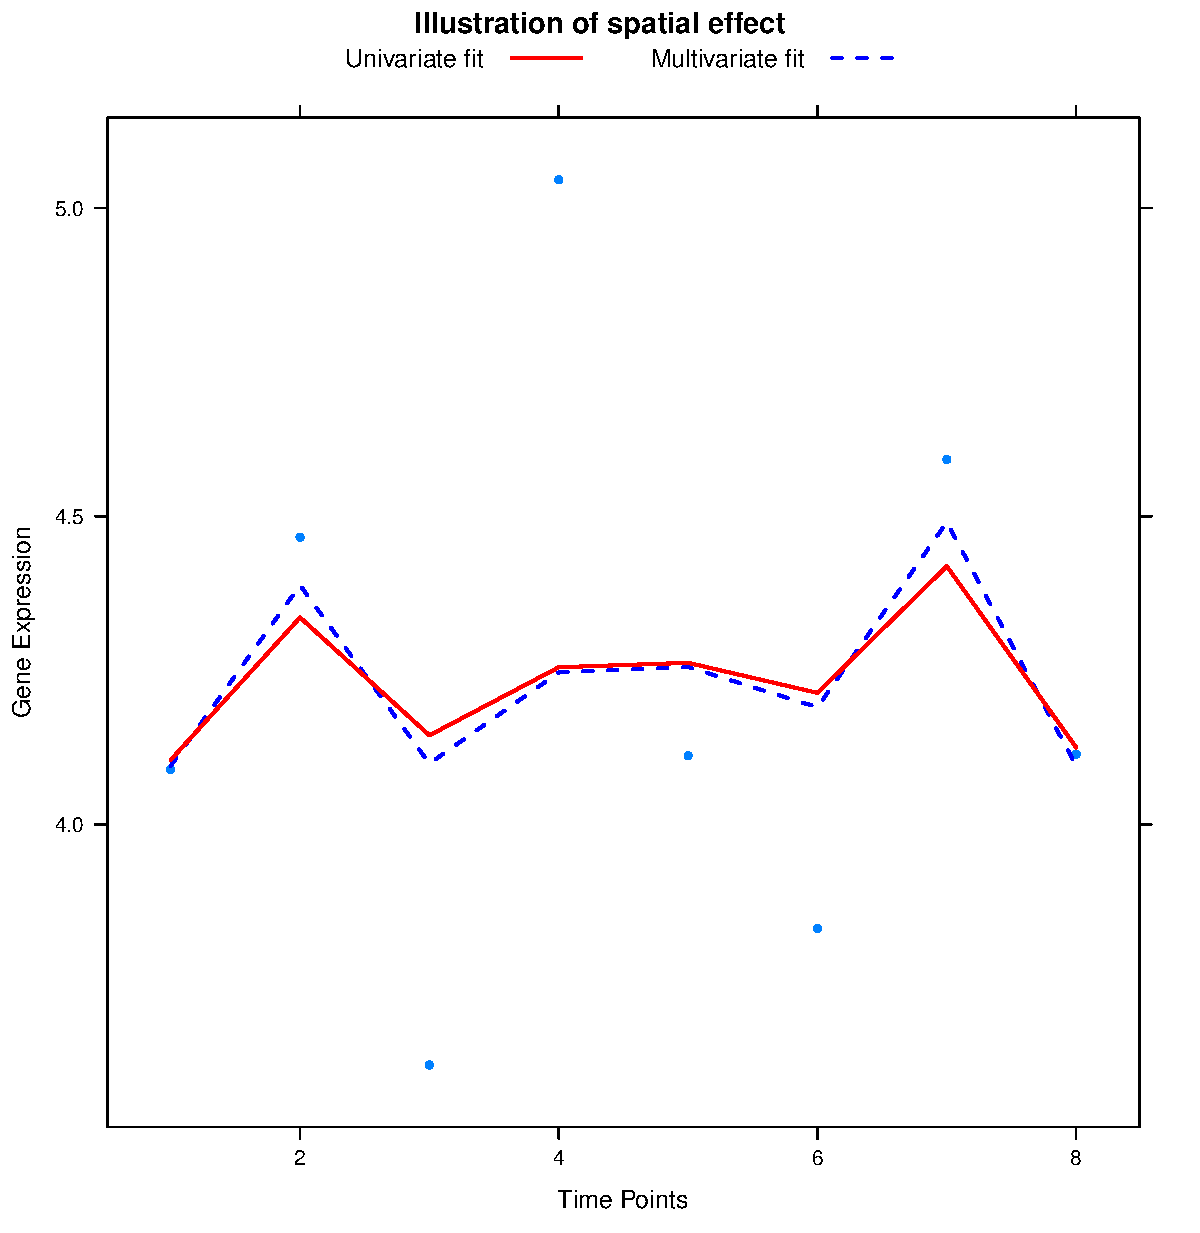
\includegraphics[scale=0.55]{Figure2.pdf}
\end{tabular}
\caption{The plot illustrates the effect of the spatial prior for one gene in single
 cell line. Gene expression is plotted against time and lines represent the
 univariate (red, solid line) and multivariate fit (blue, dashed line).}
\label{fig:spatialFit}
\end{figure}

Another striking feature of Table \ref{table:cervicalData} is the difference between the number of significant features with differential temporal expression and those with a gene dosage effect: the former exceeds the latter ( in case of the full model with different splines per cell line). In part this difference is explained by the flexibility of the splines. But also by the presence of many other regulators of gene expression (e.g. microRNA, methylation, transcription factors) that result in temporal differential expression are captured by the splines. On the other hand, comparing the analyses with a common spline more significant gene dosage effect than temporal differential expression is found. This is due to the fact that DNA copy numbers may strongly correlate with gene expression over time. Features with expression levels that do not consistently (over cell lines) co-vary with DNA copy number are missed by the common spline model (and not including the gene dosage effect).

To give some more tangible insight into the results from the analyses above, we single out the  CADM1 gene. It is among the genes with the highest significance for temporal differential expression (using Model (\ref{form.mixedModel}) with a common spline). Indeed, CADM1 is down-regulated in all four cell lines over time (confer Figure \ref{fig:CADM1}). This gene is well-known in cervical cancer to be down-regulated during progression due to an increasingly methylated promoter region \cite{Steenbergen2004, Overmeer2008}. The fits of Model (\ref{form.mixedModel}) with and without DNA copy number hardly differ. The estimate of the DNA copy number parameter (obtained with the common spline model) confirms this ($\hat{\beta}_{\mbox{{\tiny CADM1}}} = 1.1$). This suggests that the down-regulation of CADM1 is not due to a DNA copy number loss, which corresponds with previous findings (e.g \cite{Steenbergen2004}).

\begin{figure}[h!]
\centering
\begin{tabular}{c}
\includegraphics[scale=0.55]{Figure5.pdf}
\end{tabular}
\caption{Expression levels of CADM1 over time. The solid red and dashed blue
 lines are the fits of the model with and without DNA copy number parameter, 
respectively.}
\label{fig:CADM1}
\end{figure}

To contrast the results for CADM1, we focus on the SLC25A36 gene. SLC25A36 exhibits temporal differential expression (irrespective of the choice for common or different spline model). SLC25A36 is also identified as a gene with a significant DNA copy number effect with estimate $\hat{\beta}_{\mbox{{\tiny SLC25A36}}} = 1.6$. Inclusion of DNA copy number in the model improves the fit substantially (confer Figure \ref{fig:SLC25A36}, illustration on four cell lines in Figure 2.8 \cite{Supp2018}). This is seen in the Figure \ref{fig:SLC25A36} as the difference in fit for the model with and without DNA copy number. These results for SLC25A36 corroborate with existing medical literature: the gene dosage effect for this gene has already been reported in cervical cancer \cite{Wilting2008}.

\begin{figure}[h!]
\centering
\begin{tabular}{c}
\includegraphics[scale=0.55]{Figure6.pdf}
\end{tabular}
\caption{Expression levels of SLC25A36 over time points in single cell line. The
 solid red and dashed blue lines are the fits of the model with and without DNA
copy number parameter, respectively.}
\label{fig:SLC25A36}
\end{figure}

Finally, we want to assess the sensitivity of the results with respect to the choice of the prior distribution. For illustration purposes we focus on the hyperprior of the random effect $\gamma_{k,j}$. In Section \ref{estimation} we suggest to use the Gamma distribution. However, we have also implemented a mixture of a point mass at zero and Gamma distribution, which one expects to lead to more shrinkage. Model (\ref{form.mixedModel}) using different splines and a standard design matrix is refitted now with this mixture prior for the random spline effect. Application of our empirical Bayes procedure with the Gamma prior identified 421 features, while the Dirac-Gamma mixture prior selected 396 features. The latter 396 are all included in the former 421 features. The slight reduction in the number of selected features is of course due to the inclusion of the point mass at zero. The fit of both resulting models is almost identical for most features, but for some features with a slightly less flexible spline as in Figure \ref{fig:priors} (in Figure 2.9 \cite{Supp2018}, illustrates effect in all four cell lines).

\begin{figure}[h!]
\centering
\begin{tabular}{c}
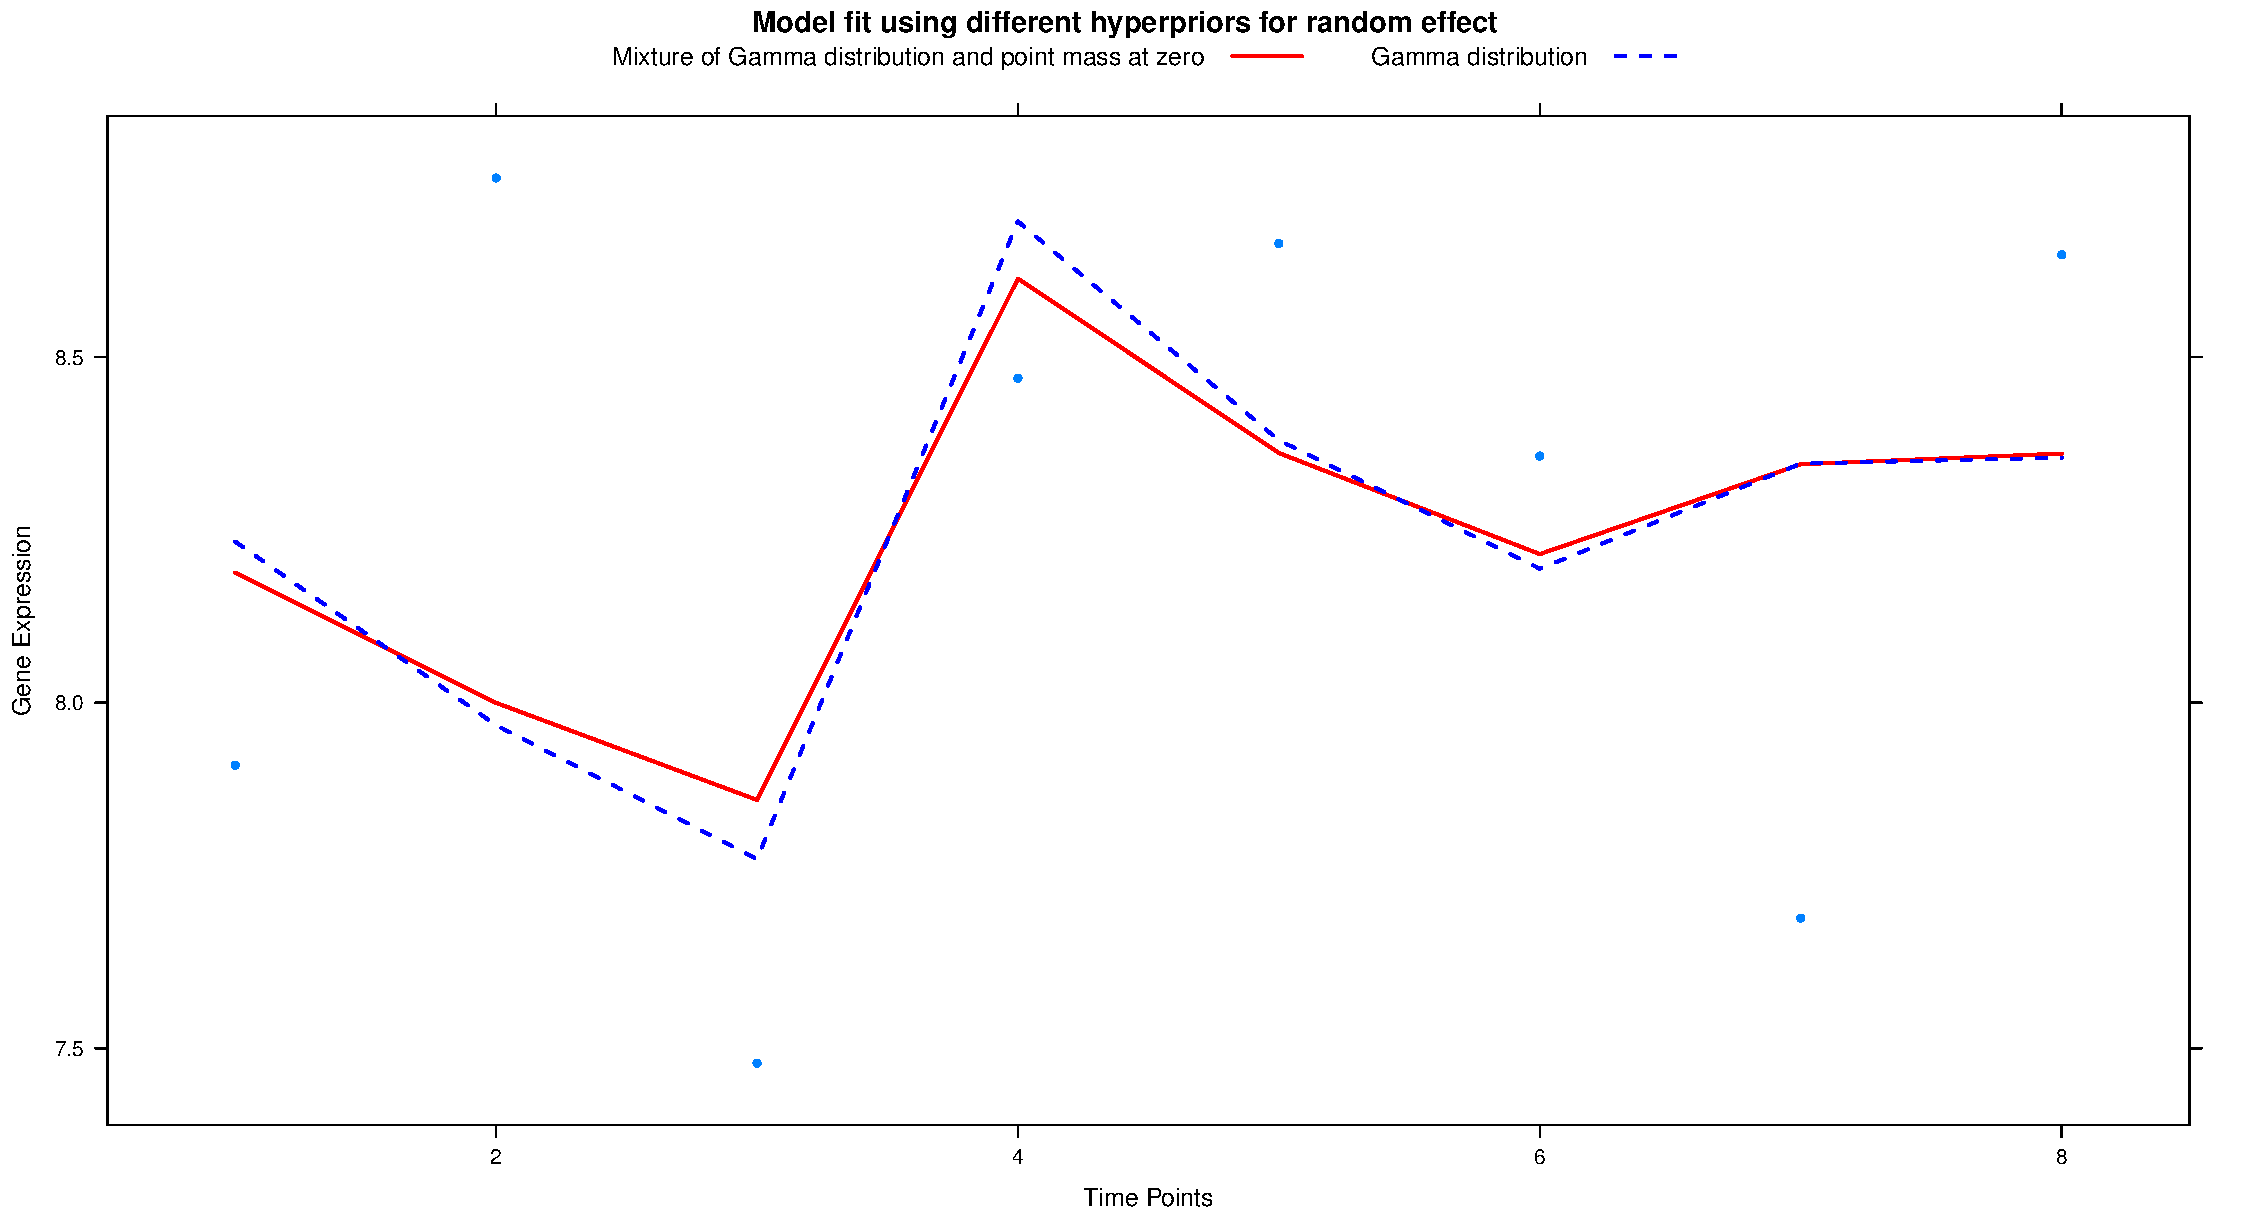
\includegraphics[scale=0.4]{Figure7.pdf}
\end{tabular}
\caption{This plot illustrates the effect of using different priors in one cell line.
 Gene expression is plotted against time (single cell line only). The
 solid red line is the fit of the model with a standard prior, while the dashed
 blue line is that of the model with an alternative prior.}
\label{fig:priors}
\end{figure}

\subsection{Head-and-neck cancer}
\label{headNeck}
To illustrate the wide applicability of our framework, we present the analysis of sequencing data from a head-and-neck cancer study endowed with a time-course set-up. \cite{Oshlack2010} noticed that there are currently no appropriate methods for the analysis of RNA-seq data from time-course experiments. The head-and-neck study aims to identify temporal differential expression due to overexpression of a particular microRNA. MicroRNAs are small 20-22nt non-coding RNAs that inhibit expression of their target genes. The microRNAs recognize these genes by their seed sequence that is complementary to a sequence in the 3' untranslated region (UTR) of the target transcripts. One gene can be targeted by multiple microRNAs and one microRNA may target a multitude of genes. It is therefore not simple to find a specific relevant target gene of a microRNA. In a previous functional screen microRNAs were identified that specifically kill head and neck cancer cells, but not normal cells \cite{Lindenbergh2013}. The respective target genes of these microRNAs were to be identified in a follow-up experiment. In this follow-up experiment cells of a squamous cell carcinoma cell line were transfected by a microRNA mimic and a control. The transfected cells were grown {\it in vitro} and sampled at six time points. Transcript levels of the $2 \times 6$ samples were sequenced. Data were mapped to the human genome and raw count data (reads) per gene transcript were used and not summarized per gene. Their normalization comprises rescaling by a the trimmed mean of each sample's library (following \cite{Oshlack2010}). Normalized data are rounded to the closest integer to retain the count interpretation of the data.


Model (\ref{form.mixedModel}) cannot be directly applied to the sequencing data, as the normal distribution is often a poor approximation for the distribution of counts. The normality assumption is replaced by the (zero-inflated) negative binomial \cite{RobinsonSmyth2007, Mark2013}: $Y_{i,j,t} \sim \mathcal{ZI}$-$\mathcal{NB}(\mu_{i, j,t}, \phi_{\varepsilon,j})$. The mean $\mu_{i,j,t}$ of the counts is (after transformation by the inverse of the link function) still modeled by the right-hand side of Model (\ref{form.mixedModel}) with assumptions on model parameters in place. Hyperparameters are then estimated via the empirical Bayes procedure previously described.

The analysis of the head-and-neck cancer data concentrates on two main questions: identification of tags with temporal variation and those different between the two conditions. To answer this, Model (\ref{form.mixedModel}) is used without the DNA copy number term (which is not included in the experiment). Common and different spline models are employed as Section \ref{cervical}. Parameter $\gamma_j$ is the main parameter of interest and the analysis compares the model with and without time effect. The optimal number of knots (again two, for both models) is determined using the procedure described in Section \ref{considerations}. Prior distributions for cell line and time effect are as in Section \ref{estimation}. Hyperparameters are estimated for each analysis separately, but only the variance of the random time effect is shrunken via the empirical Bayes procedure.

\begin{figure}[h!]
\centering
\begin{tabular}{c}
\includegraphics[scale=0.55]{Figure8.pdf} %width=6in, height=4in
\end{tabular}
\caption{The dots represent the RNA-seq tag counts plotted against time. The
 solid (red) line represents the fit of the model with different splines per group
 while the dashed (blue) line that of the model with a common spline for both
 groups.}
\label{seqdata}
\end{figure}

The number of tags with a significant (at the 5\% FDR level) temporal variation identified equals 8416 (10951) for the common (different) spline model. As observed in the analysis of the HPV-induced transformation data, the use of a different spline leads to many more findings. Again, this is explained by the improved fit due to a more flexible model. In particular, all the tags identified with the same spline model are also found by its flexible counterpart.


\subsection{Comparison}
\label{comparison}
The proposed method is compared to three well-known alternatives for significance analysis of time-course microarray data: {\tt EDGE} \cite{Storey2005}, {\tt timecourse} \cite{Tai2006}, {\tt BATS} \cite{Angelini2007, Mutarelli2008}, and a reference method. The reference method comprises a standard frequentist approach. It fits a linear mixed-effect model, while the null hypothesis is evaluated through an analysis of variance approach (anova), comparing two nested models (with and without random effects).

These competitors have not been designed for the analysis of integrative genomics studies with a time-course set-up. Hence, our method is applicable to a wider class of studies. Besides this qualitative argument, we wish to have a quantitative comparison of the methods. To this end the comparison is restricted to time-course genomics studies involving only a single molecular level. Moreover, to avoid bias of any of the methods by a particular model choice, the comparison is done on two real data sets. The first is the HPV-induced transformation data from Section \ref{cervical}, limited to the gene expression levels only. The other data set is included in the {\tt EGDE}-package \cite{Storey2005}, where gene expression has been monitored in four individuals from a control and endotoxin-treated group. Samples have been collected at five different time points: 2, 4, 6, 9 and 24 hours after treatment. One individual lacks data for the control group at two time points (4 and 6 hours). Since the {\tt timecourse} method cannot deal with missing time-points this individual is omitted from the analysis. At each time point expression levels of 800 genes are available.
\\
\\
We now briefly describe the other methods used in the comparison: {\tt EDGE}, {\tt BATS} and {\tt timecourse}. For a more detailed description please refer to the corresponding references.

{\tt EDGE} \cite{Storey2005} captures the temporal variation in the  expression levels of gene $j$ by means of a p-dimensional B-spline basis. Temporal differential expression is evaluated by an F-statistic measuring the goodness-of-fit of the null hypothesis (a flat or constant spline) in comparison to the alternative hypothesis. In the comparison {\tt EDGE} is used with default parameter settings.

{\tt timecourse} \cite{Tai2006} uses novel multivariate empirical Bayes statistic to rank time-course gene expression profiles. Gene expression in {\tt timecourse} method is assumed to follow a multivariate normal distribution with gene-specific mean and covariance. Conjugate priors are assumed on the unknown parameters. Hyperparameters of the conjugates are estimated from the data. {\tt timecourse} yields stable variance estimates by borrowing (co)variance information across genes. The posterior distribution and test statistics are obtained in an analytic form. Genes may be ranked using either Hotelling $T^2$ or $MB$-statistics. For the comparison we used the {\tt timecourse} R-package with standard settings and Hotelling $T^2$-statistic, due to the balancedness of the study design (equal number of replicates per gene).

Finally, {\tt BATS} \cite{Angelini2007} which combines characteristics from previously described methods. Similar to {\tt EDGE} gene expression variation over time is modelled by a polynomial function, while imposing a hierarchical Bayesian model on the parameters (as {\tt timecourse}). {\tt BATS} is flexible in its choice of the prior for dispersion related parameters, it offers delta, inverse Gamma and exponential priors. Significance analysis is based on the genes' Bayes factors, while multiplicity correction is addressed in Bayesian manner \cite{Abramovich2006}.
\\
\\
Sensitivity and specificity of the five aforementioned methods are compared in both data sets. Hereto knowledge of the genes with true temporal differential expression is needed. In its absence we constructed a consensus set which fulfills this role. That consensus set comprises of the features identified by all three methods. Sensitivity is then the proportion of features with temporal differential expression correctly identified as such. On the other hand, specificity is the proportion of features which are correctly identified as features without differential expression over time (hence, rightly not significant). Sensitivity and specificity of each method are assessed for various numbers of significant features.

Figure \ref{fig:sens&spec} presents the resulting sensitivity and specificity for the HPV-induced transformation data. The left panel of Figure \ref{fig:sens&spec} compares the sensitivity. While {\tt BATS}, {\tt timecourse} and {\tt EDGE} are more or less on a par, they all have a lower true positive rate than {\tt tigaR}. With respect to the specificity, the methods are more or less on a par with {\tt tigaR} having a slightly lower false positive rate than the other methods. This is confirmed (though much less pronounced) by the results from the {\tt EDGE}-package data (see in \cite{Miok2014}, Section 2.6.). For both sensitivity and specificity the methods perform similarly with {\tt tigaR} having a marginal lead.

\begin{figure}[h!]
\centering
\begin{tabular}{cc}   
\includegraphics[scale=0.4]{Figure9.pdf}
\end{tabular}
\caption{Comparison of sensitivity and specificity for {\tt tigaR}, {\tt EDGE}, {\tt BATS} and 
{\tt timecourse} on the data set of Section \ref{cervical}. The left (right) panel displays the
 sensitivity of the methods (specificity) by plotting true (false) positive rate
 against the number of significant features.}
\label{fig:sens&spec}
\end{figure}

Furthermore, we compared the reproducibility of the five methods. Hereto each data set was divided into two equally sized groups. We assessed how well the results of the two splits coincided. This boils down to the application of each method on both splits. The overlap in significant features for each method was determined.

Figure \ref{fig:reproduc} shows the reproducibility of each method on the data set from Section \ref{cervical}. It reveals that {\tt BATS} and {\tt tigaR} reproduce substantially better than the competitors. This is confirmed in the other data set (see in \cite{Supp2018} Section 2.6). The superior reproducibility is most likely a consequence of the empirical Bayes approach (borrowing of information stabilizes estimates) in {\tt tigaR} and very informative priors in {\tt BATS}. The {\tt tigaR}, {\tt BATS} and {\tt timecourse}-methods do much better than {\tt EDGE} in both data sets. The former three all exploit the Bayes principle (in different ways though) which  improves estimates of the variance parameters, while {\tt EDGE} does not.

\begin{figure}[h!]
\centering
\begin{tabular}{c}
\includegraphics[scale=0.4]{Figure10.pdf}
\end{tabular}
\caption{Reproducibility of {\tt tigaR}, {\tt EDGE}, {\tt BATS}, {\tt timecourse} and reference
 model are assessed on the data set of Section \ref{cervical}. The number of significant
 features identified in both groups are plotted against the initial number of
 features.}
\label{fig:reproduc}
\end{figure}

\section{Conclusion}
We presented a method for the analysis of integrative (onco) genomics studies with a time-course experimental design. The method identifies temporal differential gene expression while accounting for time-varying molecular covariates like DNA copy number changes. Simultaneously, the method assesses which of these covariates significantly contributes to temporal differential gene expression. The method employs a mixed model describing the temporal changes in gene expression in terms of DNA copy number and a (low-rank thin-plate) spline which captures additional temporal variation in the transcript levels. The method estimates the parameters of this model by means of an empirical Bayes procedure that `borrows information' across genes. The empirical Bayesian procedure shrinks the parameter estimates (towards zero), thus accounting for multiplicity. This shrinkage enhances the reproducibility of the results. In a direct comparison with other methods for the identification of temporal differential expression, the proposed method proved to be a strong competitor, particularly in terms of reproducibility. In addition existing methods can not incorporate additional genomics data. Furthermore, our method is straightforwardly applicable to count data resulting from RNA-seq experiments. Application to an integrative oncogenomics study, involving HPV-transformated cell lines, confirmed genes CADM1 and SLC25A36, known to be implicated in the development of cervical cancer. The presented methodology also identified other, novel and potentially interesting genes. These are currently under investigation and will be reported in a follow-up medical paper.
Preliminary pathway analysis already showed that genes identified from this dataset by {\tt tigaR} but not by the other methods were enriched for genes involved in cellular transformation.


Our ongoing research concentrates on two extensions of the proposed method. First, we are considering the inclusion of microRNA data. MicroRNAs affect expression levels post-transcriptionally. However, which microRNA targets which mRNA is only partially known. Hence, integration of temporal microRNA expression data also needs to address the problem of selecting the microRNAs targets. With the number of microRNAs known and typically measured in time-course integrative genomics studies being larger than the number of samples (\# time points $\times$ \# cell lines) this adds an additional layer of complexity to the problem.

The second extension comprises the integration of pathway information. This requires a multivariate formulation of the model for temporal changes in gene expression. Next to DNA copy number changes now the changes in transcript levels of other genes in the pathway may need to be included. A key challenge here is to `borrow information' within and between pathways.

The methodology described in this paper is implemented in the R-package {\tt tigaR} available upon request.


\chapter{Ridge estimation of the VAR(1) model and its time series chain graph from multivariate time-course omics data \\ {\footnotesize (\textit{Miok, V., Wilting, S. M. and van Wieringen, W. N., Biometrical Journal (2017), 59(1), 172-191})}}
\label{ch3:ragt2ridges}
\chaptermark{Ridge estimation of the VAR(1) model}
\label{chapter:Estimating entropy loss in Gaussian graphical models}
\graphicspath{{Chapter3/Figs/}{Chapter3/Figs/PDF/}{Chapter3/Figs/}}%

Omics experiments endowed with a time-course design may enable us to uncover the dynamic interplay among genes of cellular processes. Multivariate techniques (like VAR(1) models describing the temporal and contemporaneous relations among variates) that may facilitate this goal are hampered by the high-dimensionality of the resulting data. This is resolved by the presented ridge regularized  maximum likelihood estimation procedure for the VAR(1) model. Information on the absence of temporal and contemporaneous relations may be incorporated in this procedure. Its computational efficient implementation is discussed. The estimation procedure is accompanied with an LOOCV scheme to determine the associated penalty parameters. Downstream exploitation of the estimated VAR(1) model is outlined: an empirical Bayes procedure to identify the interesting temporal and contemporaneous  relationships, impulse response analysis, mutual information analysis, and covariance decomposition into the (graphical) relations among variates. In a simulation study the presented ridge estimation procedure outperformed a sparse competitor in terms of Frobenius loss of the estimates, while their selection properties are on par. The proposed machinery is illustrated in the reconstruction of the p53 signalling pathway during HPV-induced cellular transformation. The methodology is implemented in the \texttt{ragt2ridges} R-package available from CRAN.
\\
\\
This chapter was published as:\\
Miok, V., Wilting, S. M. and van Wieringen, W. N. (2017). Ridge estimation of the VAR(1) model and its time series chain graph from multivariate time-course omics data. \textit{Biometrical Journal}, 59(1), 172-191.

\section{Introduction}
Molecular biology aims to unravel the workings of the cell. This amounts to which and how molecules like mRNAs work together. A widely accepted paradigm assumes a modular set-up \cite{Alon2003}. Modules, called pathways, comprise groups of genes that work together to e.g. process a signal (which may then be passed on to another pathway). For some pathways it is (at least partially) known how genes interact. Often this knowledge is derived from experiments on properly working model systems. Cancer, however, is due to a (possible multiple) failure(s) at the molecular level of the cell \citep{Weinberg2006}. Such failures may cause pathways to be dysregulated in cancer cells. The gene-gene interaction pattern may thus be altered. Knowledge of the regulatory patterns of pathways in cancer cells is of paramount importance for the development of molecular medicines that specifically target the failure (or consequences thereof).

For the elucidation of the gene-gene interactions within the cancer cell we consider oncogenomics studies with a time-course set-up. The time-course set-up implies that each sample included in the study is followed over time and, at multiple time points during this period, interrogated molecularly. Time-course studies are more powerful to investigate (dynamical aspects of) the regulatory system. Consider the following representative example of a cervical cancer genomics experiment with a time-course set-up (which is analyzed later in Section \ref{sect:illustration}). The human papilloma virus (HPV), a carcinogenic entity, is introduced in normal cells, generating a HPV-immortalized cell line. In our cervical cancer experiment two cell lines are infected with HPV16 and two with HPV18 \cite{Steenbergen1996}. The resulting cell lines are shown to faithfully mimic cervical cancer development, morphologically and (epi)genetically \cite{Steenbergen2004, Wilting2006, Henken2007}. After introduction of the virus the cells are maintained in culture and go through distinct phenotypic stages to finally become fully transformed, as illustrated by their ability to grow anchorage independent. During this transformation process, which can take many population doublings, cells can be profiled at different stages of transformation. In the cervical cancer experiment cells from each cell line are  profiled by oligonucleotide microarrays at eight uniformly distributed time points. This will provide insight into the changes in expression over time underlying the cellular process of carcinogenesis. 

Statistically, the dynamics of the gene expression levels within a pathway may be described by a vector autoregressive model, abbreviated to VAR(1) model where `1' specifies the lag. The VAR(1) model specifies the distribution of the process but does not directly reveal the underlying network of (cross-)temporal and contemporaneous relations among its variates. This is captured by its associated time-series chain graph \citep{Dahlhaus2000}, which describes the conditional independencies among variates over time. The time-series chain graph suggests how molecular medicine could target the pathway.

VAR(1) models are well-studied (confer monographs \cite{Hamilton1994, Lutkepohl2005}), in particular their full maximum likelihood (ML) estimation. Little attention has been given to full ML estimation from high-dimensional data as typically arise from time-course genomics studies. To our knowledge only \cite{Abegaz2013} address this problem by augmenting the likelihood of the VAR(1) model with SCAD (smoothly clipped absolute deviation) penalties \cite{Fan2001}. Here we contrast this by considering ridge penalization instead. This is motivated from penalized estimation of Gaussian graphical models (GGM) used in the reconstruction of the gene-gene interaction network from observational genomics studies. In a vis-a-vis data-driven comparison of the lasso and ridge estimators (of \cite{Friedman2008} and \cite{Wieringen2016}, respectively) of the GGM, the latter performed (in contrast to the former) favourably in terms of loss and comparably in terms of selection properties \cite{Wieringen2016}. With the SCAD penalty being closely related to the lasso, the favourable behaviour of ridge estimation of GGM may carry over to ridge estimation of VAR(1) models and may benefit the reconstruction of their associated time-series chain graph.

The outline of the paper is as follows. First, the VAR(1) model and its properties along with its associated time-series chain graph are recapitulated. With this knowledge refreshed, the ridge penalized full ML estimator of the VAR(1) model is presented. The estimator is extended to allow the incorporation of prior knowledge on the support of both temporal and contemporaneous interactions. In both cases memory efficient evaluation of the estimator is outlined. Cross-validation (which requires minor changes to the estimator) is described to guide the choice of the penalty parameters. Then, several strategies (e.g. selection of temporal and contemporaneous relationships, mutual information, and path analysis) for down-stream exploitation of the estimated model are discussed. This is followed by a comparison of the SCAD and ridge penalized ML estimation procedures of the VAR(1) model. Finally, the presented methodology is applied to the aforementioned HPV-induced transformation study.


\section{The VAR(1) model}
Consider an experiment in which $n$ samples (cell lines) are followed over time. Of each sample $p$ variates (e.g. mRNA levels) are measured at $\mathcal{T}$ time points. The time points coincide among the samples. Let $Y_{j,t,i}$ be a random variable representing the measurement of variate $j$ in sample $i$ at time point $t$. The vector comprising the measurements of all variates of sample $i$ at time point $t$ is denoted $\mathbf{Y}_{\ast,t,i}$.

The data from the time-course experiment are modeled by a VAR(1) (first-order vector autoregressive) process:
\begin{eqnarray} \label{form.var1}
\mathbf{Y}_{\ast, t, i} \, | \, \mathbf{Y}_{\ast, t-1, i}, \ldots,  \mathbf{Y}_{\ast, 1, i}
\, \, \, = \, \, \, \mathbf{Y}_{\ast, t, i} \, | \, \mathbf{Y}_{\ast, t-1, i} & = & \nnu + \mathbf{A} \mathbf{Y}_{\ast, t-1, i} + \vvarepsilon_{\ast, t, i},
\end{eqnarray}
where $\nnu$ the $p \times 1$ intercept vector, $\mathbf{A}$ a $p \times p$ regression coefficient matrix, and $\vvarepsilon_{\ast, t, i}$ a $p \times 1$ vector with the errors. Throughout it is assumed that $\nnu = \mathbf{0}_{p \times 1}$ (data should thus be centered per variate and within-sample), $\vvarepsilon_{\ast,t,i} \sim \mathcal{N}(\mathbf{0}_{p \times 1}, \mathbf{\Sigma}_{\varepsilon})$ and $\mbox{Cov}(\vvarepsilon_{\ast,t_1,i_1}, \vvarepsilon_{\ast,t_2, i_2}) = \mathbf{0}$ if $t_1 \not=t_2$ or $i_1 \not=i_2$. Finally, the VAR(1) process is assumed to be stationary (having finite first and second moment). Under the above assumptions the mean of $\mathbf{Y}_{\ast,t,i}$ equals $\mathbf{0}_{p \times 1}$ (due to $\nnu = \mathbf{0}_{p \times 1}$). Furthermore, from model (\ref{form.var1}) it is clear that the variance of $\mathbf{Y}_{\ast,t,i}$ satisfies: $\mathbf{\Sigma}_{y}  =  \mathbf{A} \mathbf{\Sigma}_{y} \mathbf{A}^{\top} + \mathbf{\Sigma}_{\varepsilon}$, which may be solved for $\mathbf{\Sigma}_y$ explicitly in terms of $\mathbf{A}$ and $\mathbf{\Sigma}_{\varepsilon}$. Finally, the autocovariance (the covariance between the variates at one time point and some other) of the VAR(1) process is: $\mathbf{\Gamma}(\tau)  =  \mbox{Cov} \big( \mathbf{Y}_{\ast,t,i}, \mathbf{Y}_{\ast,t+\tau,i} \big) = \SSigma_y [\mathbf{A}^{\tau}]^{\top}$ for $\tau \geq 0$. Similarly, $\mathbf{\Gamma}(\tau)  = \mathbf{A}^{-\tau} \SSigma_y$ for $\tau < 0$.

The maximum likelihood (ML) estimators of the parameters of the VAR(1) model can readily be obtained. The likelihood of model (\ref{form.var1}) is, using $\mathbf{Y}_{\ast,t,i} \, | \, \mathbf{Y}_{\ast,t-1,i} \sim \mathcal{N}( \mathbf{A} \mathbf{Y}_{\ast,t-1,i}  , \SSigma_{\varepsilon})$:
%\begin{eqnarray*}
\begin{flalign*}
\resizebox{1.05\hsize}{!}{$
L(\mathbf{Y}; \mathbf{A}, \SSigma_{\varepsilon})  =  \prod_{i=1}^n \prod_{t=2}^{\mathcal{T}} \frac{1}{(2\pi)^{p/2} | \SSigma_{\varepsilon} |^{1/2} } \exp \big[ \frac{-\big( \mathbf{Y}_{\ast,t,i} - \mathbf{A} \mathbf{Y}_{\ast,t-1,i}  \big)^\top \SSigma_{\varepsilon}^{-1} \big(\mathbf{Y}_{\ast,t,i} - \mathbf{A} \mathbf{Y}_{\ast,t-1,i}  \big)}{2} \big]. \qquad
$}
\end{flalign*}
%\end{eqnarray*}
Maximization of this likelihood yields:
\begin{eqnarray*}
\widehat{\mathbf{A}} & = &  \Big[ \frac{1}{n(\mathcal{T}-1)} \sum_{i=1}^n \sum_{t=1}^{\mathcal{T}-1}  \mathbf{Y}_{\ast,t+1,i} \mathbf{Y}_{\ast,t,i}^{\top} \Big] \Big[ \frac{1}{n({\mathcal{T}}-1)} \sum_{i=1}^n \sum_{t=1}^{{\mathcal{T}}-1}  \mathbf{Y}_{\ast,t,i} \mathbf{Y}_{\ast,t,i}^{\top} \Big]^{-1},
\\
\widehat{\SSigma}_{\varepsilon} & = & \frac{1}{n \mathcal{T}}  \sum_{i=1}^n \sum_{t=2}^{\mathcal{T}}  \big[ \mathbf{Y}_{\ast,t,i} - \mathbf{A} \mathbf{Y}_{\ast,t-1,i}  \big] \big[ \mathbf{Y}_{\ast,t,i} - \mathbf{A} \mathbf{Y}_{\ast,t-1,i}  \big]^{\top}.
\end{eqnarray*}
Thus, $\mathbf{A}$ is estimated by the product of the sample estimates  of the autocovariance $\mathbf{\Gamma}(-1)$ and the variance $\mathbf{\Gamma}(0)$, while $\SSigma_{\varepsilon}$ is estimated by the sample residual covariance matrix. Both ML estimators (of $\mathbf{A}$ and $\mathbf{\Sigma}_{\varepsilon}$) are biased but consistent \cite{Nicholls1988, Lutkepohl2005}. Finally, we remark that the OLS (ordinary least squares) and ML estimators of $\mathbf{A}$ coincide (in the unpenalized case).

The VAR(1) model is well-known and only those properties relevant to the remainder of the paper have been recapitulated above. The reader is referred to the standard textbooks of \cite{Hamilton1994}
and \cite{Lutkepohl2005} for more on the VAR(1) model.


\subsection{Conditional independence}
The conditional independencies among the variates of $\mathbf{Y}_{\ast,t,i}$ as implied by the VAR(1) model are represented by a conditional independence graph \citep{Whittaker1990}. Such a graph $\mathcal{G}$ is a pair $(\mathcal{V}, \mathcal{E})$, where $\mathcal{V}$ is a finite set of nodes (also called vertices) of graph components (here variates $j=1, \ldots, p$). The $\mathcal{E}$ is a subset of $\mathcal{V} \times \mathcal{V}$ of ordered pairs of nodes, called edges of the graph. The nodes are the entities of interest and the edges represent the relationships among the entities. If both ordered pairs $(v_1, v_2)$ and $(v_2, v_1)$ belong to $\mathcal{E}$, the graph $\mathcal{G}$ has an undirected edge between $v_1$ and $v_2$. The edge is directed if only one of the two is in $\mathcal{E}$. An undirected graph comprises undirected edges only. An undirected graph  $\mathcal{G}$ is a conditional independence graph for the VAR(1) process if $(v_1, v_2) \not\in \mathcal{E} \Longleftrightarrow Y_{v_1, \ast, i} \independent Y_{v_2, \ast, i} \, | \, \mathbf{Y}_{\mathcal{V} \setminus \{v_1, v_2\}, \ast, i}$, where, e.g. $Y_{v, \ast, i}$ represents the subprocess of variate $v$ over time.

Helpful in the understanding of the relation between the parameters and conditional independencies of a VAR(1) process is a time series chain graph, which represents the local (time-wise) conditional independencies of the process. Following \cite{Dahlhaus2000, Dahlhaus2003}, a time series chain graph $\mathcal{G}_{TS} = (\mathcal{V}_{TS}, \mathcal{E}_{TS})$ is a mixed graph, a graph containing both directed and undirected edges. The vertex set $\mathcal{V}_{TS}$ comprises of the variates at all time points, i.e. $\mathcal{V}_{TS} = \{\ldots, \mathcal{V}_{t-1}, \mathcal{V}_{t}, \mathcal{V}_{t+1}, \ldots\}$, while the edge set $\mathcal{E}_{TS}$ constitutes of all temporal and contemporaneous edges. Temporal edges are directed and (in the VAR(1) model) connect nodes from $\mathcal{V}_{t}$ to that of $\mathcal{V}_{t+1}$ for any $t \in \mathbb{Z}$. Presence or absence of these edges correspond to nonzero or zero (respectively) elements of $\mathbf{A}$, where the latter implies the conditional independence relation $Y_{j_1, t, i} \independent Y_{j_2, t+1, i} \, | \, \mathbf{Y}_{\ast, t, i} \setminus Y_{j_1, t, i}$. Contemporaneous edges are undirected and connect the nodes within  $\mathcal{V}_{t}$. Presence or absence of contemporaneous edges match with nonzeros or zeros in the error precision matrix $\mathbf{\Sigma}_{\varepsilon}^{-1}$, where the zeros imply $Y_{j_1, t, i} \independent Y_{j_2, t, i} \, | \, \mathbf{Y}_{\ast, t, i} \setminus \{ Y_{j_1, t, i}, Y_{j_2, t, i} \}, \mathbf{Y}_{\ast, t-1, i}$.


Global conditional independence among subprocesses of the VAR(1) process hold if the partial correlations among the subprocesses vanish (Theorem 3.1 of \cite{Dahlhaus2003}). Proposition 2.7 of \cite{Dahlhaus2003} specifies a parametric criterion for the vanishing partial correlations in multivariate time series. For the VAR(1) process these results imply that $Y_{j_1, \ast, i} \independent Y_{j_2, \ast, i} \, | \, \mathbf{Y}_{\mathcal{V} \setminus \{j_1, j_2\}, \ast, i}$ if
\begin{compactitem}
\item[\textit{a)}] $(\mathbf{\Sigma}_{\varepsilon}^{-1})_{j_1, j_2} \qquad  \, \, = 0$, and
\item[\textit{b)}] $(\mathbf{A}^{\top}  \mathbf{\Sigma}_{\varepsilon}^{-1})_{j_1, j_2}  \, \, \, \, \,
= \sum_{j=1}^p (\mathbf{A})_{j, j_1}  (\mathbf{\Sigma}_{\varepsilon}^{-1})_{j, j_2} \qquad \qquad  = 0$, and
\item[\textit{c)}] $(\mathbf{\Sigma}_{\varepsilon}^{-1} \mathbf{A})_{j_1, j_2} \quad \, \, \, = \sum_{j=1}^p (\mathbf{A})_{j, j_2} (\mathbf{\Sigma}_{\varepsilon}^{-1})_{j, j_1} \qquad \qquad = 0$, and
\item[\textit{d)}] $(\mathbf{A}^{\top} \mathbf{\Sigma}_{\varepsilon}^{-1} \mathbf{A})_{j_1, j_2}  = \sum_{j, j'=1}^p (\mathbf{A})_{j, j_1} (\mathbf{\Sigma}_{\varepsilon}^{-1})_{j, j'} (\mathbf{A})_{j', j_2} = 0$.
\end{compactitem}
The parametric criteria can be translated to the time series chain graph: subprocesses $Y_{j_1, \ast, i}$ and $Y_{j_2, \ast, i}$ are conditionally independent if there is \textit{a)} no contemporaneous edge between $j_1$ and $j_2$, \textit{b)} no temporal edge from $j_1$ to any $j$ (i.e. no $(\mathbf{A})_{j, j_1} \not= 0$) with an contemporaneous edge to $j_2$, \textit{c)} no temporal edge from $j_2$ to any $j$ with a contemporaneous edge to $j_1$, and \textit{d)} no temporal edges from $j_1$ and $j_2$ to any $j$ and $j'$ that are connected contemporaneously. Hence, conditional independencies between subprocesses can be read off the time series chain graph.

\section{Ridge estimation of the VAR(1) model} \label{sect:ridgeEstimation}

In this section the parameters of the VAR(1) model (\ref{form.var1}) with $\nnu = \mathbf{0}_{p \times 1}$ (requiring variate-wise and within-sample zero-centering of the data) are estimated from high-dimensional data by means of ridge penalized likelihood maximization. The resulting estimators are shown to be efficiently computable from high-dimensional data. Moreover, the estimators may be endowed with a `data augmentation' and Bayesian interpretation. Finally, the ridge estimation procedure is modified to allow prior knowledge on the support of temporal (Section \ref{sect:ridgeWithTemporalSupport}) and contemporaneous (Section \ref{sect:ridgeWithContemporaneousSupport}) edges of time-series chain graph.

\subsection{Ridge maximum likelihood}

The log-likelihood augmented with ridge penalties  (rewritten as e.g. \\$\lambda_a \| \mathbf{A} \|_2^2 = \lambda_a \sum_{j_1, j_2 = 1}^p [(\mathbf{A})_{j_1, j_2}]^2 = \lambda_a \mbox{tr}[\mbox{vec}(\mathbf{A})^\top \mbox{vec}(\mathbf{A})]$) for $\mathbf{A}$ and $\mathbf{\Sigma}_{\varepsilon}$ is:
%\begin{eqnarray*}
\begin{flalign*}
\resizebox{.3\hsize}{!}{$
\mathcal{L}^{\mbox{{\tiny pen}}} (\mathbf{Y};  \mathbf{A}, \mathbf{\Omega}_{\varepsilon}; \lambda_a, \lambda_{\omega}, \mathbf{A}_0, \mathbf{\Omega}_0)$} & = & \resizebox{.6\hsize}{!}{$\log[ L(\mathbf{Y}; \mathbf{A}, \mathbf{\Omega}_{\varepsilon}) ] - \frac{n (\mathcal{T} - 1)}{2} \lambda_{\omega}  \mbox{tr}  [ (\mathbf{\Omega}_{\varepsilon} - \mathbf{\Omega}_0)^\top (\mathbf{\Omega}_{\varepsilon} - \mathbf{\Omega}_0)]$} \qquad \qquad \qquad \quad 
\\
&  &  \resizebox{.6\hsize}{!}{$ - \frac{n (\mathcal{T} - 1)}{2} \lambda_a  \mbox{tr}\{ [\mbox{vec}(\mathbf{A}) - \mbox{vec}(\mathbf{A}_0)]^\top [\mbox{vec}(\mathbf{A}) - \mbox{vec}(\mathbf{A}_0)] \},$} \qquad \qquad \qquad  \quad 
\end{flalign*}
%\end{eqnarray*}
in which $\mathbf{\Omega}_{\varepsilon} = \mathbf{\Sigma}_{\varepsilon}^{-1}$. The $p \times p$ matrices $\mathbf{A}_0$ and $\mathbf{\Omega}_0$ are so-called target matrices. The ridge estimates of $\mathbf{A}$ and  $\mathbf{\Omega}_{\varepsilon}$ are shrunken (with increasing values of the penalty parameters) towards these matrices. The target matrices may represent user-specified prior knowledge on the parameters. In the envisioned usage $\mathbf{A}_0$ and $\mathbf{\Omega}_0$ are estimated from a pilot study or from publicly available data of a related disease/organ/organism and plugged in as targets when estimating the VAR(1) model from the study at hand. In case of the error precision matrix, \cite{Wieringen2016} introduce a target for $\mathbf{\Omega}_{\varepsilon}$ to ensure that the estimate is shrunken towards a well-defined, positive definite precision matrix. In the remainder $\mathbf{A}_0$ and $\mathbf{\Omega}_0$ are included in the estimators, but set equal to zero in simulation (to ensure a fair comparison) and application (no pilot data at hand). 


Maximization of the ridge penalized log-likelihood proceeds as usual. Take the derivative of the penalized log-likelihood with respect to $\mbox{vec}(\mathbf{A})$ and equate this derivative to zero to obtain the estimating equation of $\mathbf{A}$. Solve the estimating equation for $\mathbf{A}$ to arrive at the ridge ML estimator:
\begin{eqnarray}
\nonumber
\mbox{vec}[ \hat{\mathbf{A}}(\lambda) ] & = &  \Big[ n (\mathcal{T} - 1) \lambda_a \mathbf{I}_{p^2 \times p^2}  + \sum_{i=1}^n \sum_{t=2}^{\mathcal{T}} \big( \mathbf{Y}_{\ast,i,t-1} \mathbf{Y}_{\ast,i,t-1}^{\top} \otimes \mathbf{\Omega}_{\varepsilon} \big) \Big]^{-1}
\\
\label{form.ridgeMLestimator}
& & \times \, \Big[n (\mathcal{T} - 1) \lambda_a \mbox{vec}(\mathbf{A}_0) + \sum_{i=1}^n \sum_{t=2}^{\mathcal{T}} \big( \mathbf{Y}_{\ast,i,t-1}  \otimes \mathbf{\Omega}_{\varepsilon} \big) \mathbf{Y}_{\ast,i,t} \Big],
\end{eqnarray}
where $\otimes$ denotes the Kronecker product \cite{Loan2000}. This estimator involves $p^2 \times p^2$ dimensional matrices, making 
the computation of Estimator (\ref{form.ridgeMLestimator}) impractical even for modestly sized pathways. But numerical evaluation of the ridge ML estimator \textit{can} be done efficiently when the estimator is reformulated algebraically. Hereto recall the following properties of the Kronecker product (confer \cite{Harville2008}). Let $\mathbf{A}$, $\mathbf{B}$ and $\mathbf{C}$ be $p \times p$ dimensional symmetric matrices, $\mathbf{V}_x \mathbf{D}_x \mathbf{V}_x^{\top}$ the eigen-decomposition of matrix $\mathbf{X} = \mathbf{A}, \mathbf{B}$ or $\mathbf{C}$, and $\lambda \in \mathbb{R}$. Then:
\begin{compactitem}
\item[i)] $\mathbf{A} \otimes \mathbf{B} + \mathbf{B} \otimes \mathbf{C}  = (\mathbf{A} + \mathbf{B}) \otimes \mathbf{C}$,

\item[ii)] $(\mathbf{A}^{\top} \otimes \mathbf{B}) \mbox{vec}(\mathbf{C}) = \mbox{vec} (\mathbf{B} \mathbf{C} \mathbf{A})$,

\item[iii)] $\lambda \mathbf{I}_{p^2 \times p^2 } + \mathbf{A} \otimes \mathbf{B} =
(\mathbf{V}_a \otimes \mathbf{V}_{b}) (\lambda \mathbf{I}_{p^2 \times p^2}  +  \mathbf{D}_a \otimes \mathbf{D}_{b}) (\mathbf{V}_a^{\top} \otimes \mathbf{V}_{b}^{\top})$.
\end{compactitem}
Application of the first two properties yields:
\begin{eqnarray*}
\mbox{vec}[ \hat{\mathbf{A}}(\lambda_{a}) ] & = &  [ \lambda_a \mathbf{I}_{p^2 \times p^2}  + \hat{\mathbf{\Gamma}}(0) \otimes \mathbf{\Omega}_{\varepsilon}  ]^{-1}
\{ \lambda_a \mbox{vec}(\mathbf{A}_0) +
\mbox{vec} [ \mathbf{\Omega}_{\varepsilon} \hat{\mathbf{\Gamma}}(-1) ] \}.
\end{eqnarray*}
Using the second and third property we get:
%\begin{eqnarray*}
\begin{flalign*}
\mbox{vec}[ \hat{\mathbf{A}}(\lambda_{a}) ]  =  \mbox{vec} \big[ \mathbf{V}_{\omega} \big( \mbox{vec} \{ \mbox{diag}[ (\lambda_a \mathbf{I}_{p^2 \times p^2}  +  \mathbf{D}_{\gamma_0} \otimes \mathbf{D}_{\omega})^{-1} ] \} \circ \mbox{vec}( \mathbf{V}_{\omega}^{\top}  \mathbf{Z} \mathbf{V}_{\gamma_0} ) \big)
\mathbf{V}_{\gamma_0}^{\top} \big],
\end{flalign*}
%\end{eqnarray*}
in which $\mbox{vec}(\mathbf{Z}) = \lambda_a \mbox{vec}(\mathbf{A}_0) + \mbox{vec} [ \mathbf{\Omega}_{\varepsilon} \hat{\mathbf{\Gamma}}(-1)]$ and $\circ$ denotes the Hadamard or element-wise product.

The limiting behaviour of the ridge ML estimator of $\mathbf{A}$  with respect to the penalty parameter $\lambda_a$ is as expected. Given $\mathbf{\Omega}_{\varepsilon}$, as $\lambda_a \downarrow 0$ the ridge ML estimator $\hat{\mathbf{A}}(\lambda_a)$ converges to the unpenalized ML estimator of $\mathbf{A}$ (assuming it is well-defined). To evaluate the other limit, $\lambda_a \rightarrow \infty$, note that the eigenvalues of $[ \lambda_a \mathbf{I}_{p^2 \times p^2}  + \hat{\mathbf{\Gamma}}(0) \otimes \mathbf{\Omega}_{\varepsilon}  ]^{-1}$ equal $1 / [ \lambda_a + (\mathbf{D}_{\gamma})_{j_1, j_1} (\mathbf{D}_{\gamma})_{j_2, j_2}]$ for $j_1, j_2=1, \ldots, p$. Consequently, $\lim_{\lambda_a \rightarrow \infty} \hat{\mathbf{A}}(\lambda_a) = \mathbf{A}_0$, again given $\mathbf{\Omega}_{\varepsilon}$.

Note that the ridge LS (Least Squares) estimator is obtained from Equation (\ref{form.ridgeMLestimator}) by setting $\mathbf{\Omega}_{\varepsilon} = \mathbf{I}_{p \times p}$ and simplifies to:
\begin{eqnarray} \label{form.ridgeLSestimator}
\hat{\mathbf{A}}(\lambda_{a}) & = & [ \lambda_a \mathbf{A}_0 + \hat{\mathbf{\Gamma}}(-1) ] [ \lambda_a \mathbf{I}_{p \times p} +  \hat{\mathbf{\Gamma}}(0) ]^{-1}.
\end{eqnarray}
Clearly, the ridge LS estimator does not involve $\mathbf{\Omega}_{\varepsilon}$. This fact will be exploited to initiate the ridge ML estimation of $\mathbf{A}$ and $\mathbf{\Omega}_{\varepsilon}$.

The VAR(1) model may be viewed as a system of Seemingly Unrelated Regressions (SUR) \citep{Zellner1962}, for which \cite{Zellner1962} showed that the LS and ML estimators of the regression coefficients ($\mathbf{A}$) coincide. Clearly, the ridge LS and ML estimators of $\mathbf{A}$ need not be equal. This can be understood as follows. It is well-known that in the presence of parameter constraints ML and LS estimators of regression coefficient need not coincide. In particular, \cite{Lutkepohl2005} shows this for the VAR(1) with linear equality constraints on $\mathbf{A}$. As the problem of maximization of the ridge penalized log-likelihood can be reformulated as a constrained estimation problem, it is readily understood that the ridge ML and LS  estimators need not coincide.

To derive the ridge ML estimator of $\mathbf{\Omega}_{\varepsilon}$, write
\begin{eqnarray*}
\mathbf{S}_{\varepsilon} & = &
\frac{1}{n (\mathcal{T} - 1)}  \sum_{i=1}^n \sum_{t=2}^{\mathcal{T}} 
\big[ \mathbf{Y}_{\ast,t,i} - \mathbf{A} \mathbf{Y}_{\ast,t-1,i}  \big]
\big[ \mathbf{Y}_{\ast,t,i} - \mathbf{A} \mathbf{Y}_{\ast,t-1,i}  \big]^{\top}.
\end{eqnarray*}
The loss function for $\mathbf{\Omega}_{\varepsilon}$ is then proportional to:
%\begin{eqnarray*}
\begin{flalign*}
{\textstyle\frac{1}{2}} n (\mathcal{T} - 1) \log| \mathbf{\Omega}_{\varepsilon} |   -  {\textstyle\frac{1}{2}} n (\mathcal{T} - 1)  \mbox{tr} (\mathbf{S}_{\varepsilon}  \mathbf{\Omega}_{\varepsilon} )
- {\textstyle\frac{1}{2}} n (\mathcal{T} - 1)  \lambda_{\omega}  \mbox{tr}  [ (\mathbf{\Omega}_{\varepsilon} - \mathbf{\Omega}_0)^\top (\mathbf{\Omega}_{\varepsilon} - \mathbf{\Omega}_0)].
%\end{eqnarray*}
\end{flalign*}
The optimum for this loss function is (confer \citealt{Wieringen2016}):
\begin{eqnarray} \label{form.ridgePrecision}
\hat{\mathbf{\Omega}}_{\varepsilon} (\lambda_{\omega}) & = & \big\{ \big[ \lambda_{\omega} \mathbf{I}_{p \times p} + {\textstyle\frac{1}{4}} (\mathbf{S}_{\varepsilon} - \lambda_{\omega} \mathbf{\Omega}_0)^2 ]^{1/2} + {\textstyle\frac{1}{2}} (\mathbf{S}_{\varepsilon} - \lambda_{\omega} \mathbf{\Omega}_0) \big\}^{-1}.
\end{eqnarray}
In \citep{Wieringen2016} it is shown that this solution is positive definite for $\lambda_{\omega} \in (0, \infty)$, \\ $\lim_{\lambda_{\omega} \downarrow 0} \hat{\mathbf{\Omega}}_{\varepsilon} (\lambda_{\omega}) = \mathbf{S}_{\varepsilon}^{-1}$ (if it is well-defined) and $\lim_{\lambda_{\omega} \rightarrow \infty} \hat{\mathbf{\Omega}}_{\varepsilon} (\lambda_{\omega}) =
\mathbf{\Omega}_0$. Given $\mathbf{A}$, these results directly apply here.

Joint ridge ML estimation of $\mathbf{A}$ and $\mathbf{\Sigma}_{\varepsilon}$ may now be performed by iteratively estimating them individually keeping the other temporarily fixed. Pseudo-code of this iterative procedure can found in the Box 1. The convergence of this iterative procedure is warranted by, e.g. Lemma 1 of \cite{Oberhofer1974} or Proposition A.3 of \cite{Lauritzen1996}. These results apply directly here as the augmentation of the log-likelihood by the two ridge penalties does not affect the continuity of the loss function. Finally, the concavity of ridge penalized log-likelihood implies that the convergence is towards a global maximum.

\begin{minipage}[h]{\textwidth}
\begin{center}
\fbox{\parbox{13cm}{
\vspace{0.2cm}
{\it Box 1:} Ridge ML estimation of the parameters of the VAR(1) model. \vspace{0.2cm}
\\
\textbf{Initiate}
\newline
Obtain an initial estimate $\hat{\mathbf{A}}^{(0)}(\lambda_a)$ of $\mathbf{A}$ from the ridge OLS estimator.
\vspace{0.2cm}
\newline
\textbf{Iterate}
\newline
For $k=1, \ldots, k_{\mbox{{\tiny max}}}$ iterate the following steps:
% \\
\begin{compactitem}
\item[1)] Use the latest estimate of $\mathbf{A}$, $\hat{\mathbf{A}}^{(k-1)}(\lambda_a)$, to calculate the sample error covariance matrix  $\mathbf{S}_{\varepsilon}^{(k)}$. Given $\mathbf{S}_{\varepsilon}^{(k)}$, the ridge ML precision estimator yields the updated estimate of $\mathbf{\Omega}_{\varepsilon}$,  $\hat{\mathbf{\Omega}}_{\varepsilon}^{(k)} (\lambda_{\omega})$.

\item[2)] Get $\hat{\mathbf{A}}^{(k)}(\lambda_a)$ from
the ridge ML estimator of $\mathbf{A}$ with $\hat{\mathbf{\Omega}}_{\varepsilon}^{(k)} (\lambda_{\omega})$ substituted for $\mathbf{\Omega}_{\varepsilon}$.
\end{compactitem}
\mbox{ }
\vspace{-0.2cm}
\newline
\textbf{Terminate}
\newline
Iterate the previous step, until convergence.
\vspace{0.2cm}
}
}
\end{center}
\end{minipage}
\mbox{ }

Finally, one may consider replacing $\hat{\mathbf{\Gamma}}(0)$
in the ridge ML estimator by: \\$\frac{1}{n \mathcal{T}} \sum_{i=1}^n \sum_{t=1}^{\mathcal{T}} \mathbf{Y}_{\ast,t,i} \mathbf{Y}_{\ast,t,i}^{\top}$. This estimator of $\mathbf{\Gamma}(0)$ does not exclude $t=1$ in the inner summation above. As such it is more efficient. As $\mathcal{T}$ is usually small in omics studies with a time-course set-up, this efficiency gain may be considerable.



\subsection{Interpretations}
Let us try to understand the effect of ridge penalty on the estimation of $\mathbf{A}$ within the VAR(1) model (assuming $\mathbf{A}_0 = \mathbf{0}$ to simplify the argument, which is analogous but less elegant for non-zero target choices). As the ridge estimator is the product of a lag one autocovariance estimate and the inverse of a biased covariance estimate, consider the related object: $\mathbf{A}(\lambda) = \GGamma(-1) [\GGamma(0) + \lambda \mathbf{I}_{p \times p}]^{-1}  =  \mathbf{A} \SSigma_y (\SSigma_y + \lambda \mathbf{I}_{p \times p})^{-1}$. Define a new stochastic process by convoluting the VAR(1) process with white noise: $\mathbf{Z}_{\ast, t, i}   =  \mathbf{Y}_{\ast, t, i} + \ddelta_{\ast,  t, i}$, with $\mathbf{Y}_{\ast, t, i}$ as in the original process (\ref{form.var1}) and $\ddelta_{\ast, t, i} \sim \mathcal{N}(\mathbf{0}_{p \times 1}, \lambda \mathbf{I}_{p \times p})$. The variance of this process is: $\SSigma_y + \lambda \mathbf{I}_{p \times p}$ and $\mathbf{Z}_{\ast, t, i}$ has the same autocovariance as $\mathbf{Y}_{\ast, t, i}$. $\mathbf{A}(\lambda)$ is then the product of the autocovariance with lag -1 and inverse of the variance of $\mathbf{Z}_{\ast, t, i}$. Inclusion of the ridge penalty could thus be thought of as adding noise to the process. This `adding noise' interpretation of the ridge ML estimator of $\mathbf{A}$ is confirmed when noting that this estimator can be obtained by data augmentation. Hereto simply augment the data array $\mathbf{Y}$ with extra multivariate time series to have dimensions $p \times \mathcal{T} \times (n + n)$. The extra time series comprises white noise distributed as $\mathcal{N}(\mathbf{0}_{p \times 1}, \lambda_a \mathbf{I}_{p \times p})$. The expectation of the variance and lag one covariance estimators constructed from the $2n$ individuals is then $\frac{1}{2} [ \mathbf{\Gamma}(0) + \lambda_a \mathbf{I}_{p \times p} ]$ and $\frac{1}{2} \mathbf{\Gamma}(-1)$, respectively. The ridge ML estimator of $\mathbf{A}$ can thus be thought of as resulting from `white noise' data augmentation.

The ridge estimator of $\mathbf{\Sigma}_{\varepsilon}$ could be endowed with a similar `data augmentation' interpretation. Hereto consider its estimator (the inverse of Equation (\ref{form.ridgePrecision})) with $\mathbf{\Omega}_0 = \mathbf{0}_{p \times p}$. The estimator is then a weighted sum of the sample covariance matrix and the (matrix-version of the) power mean of $\mathbf{S}_{\varepsilon}$ and $\sqrt{\lambda_{\omega}} \mathbf{I}_{p \times p}$. This estimator could thus be arrived at when the set of estimated residual vectors are augmented with vectors sampled from a multivariate normal with covariance equal to the aforementioned power mean. In contrast to the data augmentation of the ridge estimator of $\mathbf{A}$, these additional residual vectors are not completely uninformative but represent a compromise between white noise and the observed data (as forged by the power mean). A nonzero target precision matrix only affects this compromise, not the interpretation of data augmentation.

The ridge ML estimators of $\mathbf{A}$ and $\mathbf{\Omega}_{\varepsilon}$ both have a Bayesian interpretation. A normal prior on the elements of $\mathbf{A}$, i.e. $\mbox{vec}(\mathbf{A}) \, | \, \mathbf{\Omega}_{\varepsilon} \sim \mathcal{N}( \mathbf{0}_{p^2}, \lambda_a^{-1} \mathbf{I}_{p^2 \times p})$, produces a posterior mean that coincides with its ridge estimator: $\mathbb{E} ( \mathbf{A} \, | \, \mathbf{Y}, \mathbf{\Omega}_{\varepsilon}) =  \hat{\mathbf{A}}(\lambda_a)$ (confer \cite{Lutkepohl2005}). This assumes a zero target, but the derivation of \cite{Lutkepohl2005} are analogous for a nonzero target (that would correspond to a non-zero mean of the normal prior). Similarly, set a Wishart prior on the precision: $\mathbf{\Omega}_{\varepsilon} \sim \mathcal{W}([ 4 n^2 \lambda_{\omega} \mathbf{I}_{p \times p} + n^2 \mathbf{S}_{\varepsilon}^2 ]^{-1/2}, n)$. This yields a normal-Wishart posterior with mean $\mathbb{E} (\mathbf{\Omega}_{\varepsilon} \, | \, \mathbf{S}_{\varepsilon}) = \widehat{\mathbf{\Omega}}_{\varepsilon}(\lambda_a)$, showing that the ridge precision estimator may also be motivated from a Bayesian perspective. The appearance of $\mathbf{S}_{\varepsilon}$ in the prior of $\mathbf{\Omega}_{\varepsilon}$ has an empirical Bayes flavour with the penalty parameter $\lambda_{\omega}$ then weighing how much the scale parameter of the Wishart prior borrows from the non- and from the fully informative case. This derivation uses a zero target precision matrix, but is similar for a nonzero one only making calculations more cumbersome.

\subsection{Known temporal conditional independencies} \label{sect:ridgeWithTemporalSupport}

Prior knowledge of the temporal relations among genes may be available. For instance, it may be known whether the expression levels of one gene at time $t$ affects (or not) those of another gene at the next instance. Such information is reflected in the (non-)zero entries of $\mathbf{A}$. Alternatively, posterior to the estimation of $\mathbf{A}$ one may wish to decide on its (non-)zero elements (a procedure to this end is detailed in Section \ref{sect.supportDetermination}). Afterwards it may be worthwhile to obtain a final (and possibly less biased) estimate of $\mathbf{A}$ incorporating the inferred temporal conditional independencies as zero elements in $\mathbf{A}$.

Knowledge on the support $\mathbf{A}$ can be formulated as linear equality constraints on $\mathbf{A}$. We discuss how this is incorporated in the ridge ML estimation of the VAR(1) model. Let the linear equality constraints on $\mathbf{A}$ be given by $\mathbf{C} \, \mbox{vec}(\mathbf{A}) = \mathbf{d}$, where $\mathbf{C}$ and $\mathbf{d}$ are $q \times p^2$ and $q \times 1$ dimensional matrices and $q$ the number of constraints. The ridge ML estimator of $\mathbf{A}_c$, the constrained version of $\mathbf{A}$, solves:
\begin{eqnarray} \label{form.constrRidgeVAR1LL}
\max_{\{\mathbf{A}_c \, : \, \mathbf{C} \, \mbox{vec}(\mathbf{A}_c) = \mathbf{d}\}} \mathcal{L}^{\mbox{{\tiny pen}}} (\mathbf{Y}; \mathbf{A}_c, \mathbf{\Omega}_{\varepsilon}; \lambda_a, \lambda_{\omega}, \mathbf{A}_0, \mathbf{\Omega}_0).
\end{eqnarray}
Lagrange's method (employing the dual of problem \ref{form.constrRidgeVAR1LL}) is used to solve this maximization problem. This yields:
\begin{eqnarray}
\nonumber \mbox{vec}[\hat{\mathbf{A}}_c (\lambda_a)] & = &  \mbox{vec}[ \hat{\mathbf{A}}(\lambda_a) ] +  \big[ \lambda_a \mathbf{I}_{p^2 \times p^2}  + \hat{\mathbf{\Gamma}}(0) \otimes \mathbf{\Omega}_{\varepsilon} \big]^{-1}
\\
& & \label{form.ridgeAhat.constrained}  \mathbf{C}^{\top} \{ \mathbf{C} [ \lambda_a \mathbf{I}_{p^2 \times p^2}  + \hat{\mathbf{\Gamma}}(0) \otimes \mathbf{\Omega}_{\varepsilon} ]^{-1}  \mathbf{C}^{\top}  \}^{-1} \{\mathbf{C} \mbox{vec}[ \hat{\mathbf{A}}(\lambda_a) ] - \mathbf{d} \}.
\end{eqnarray}
in which $\hat{\mathbf{A}}(\lambda_a)$ is the unconstrained ridge ML estimate.

To impose a null structure on $\mathbf{A}$ denote by $\mathcal{V}_0 \subset \{1, 2, \ldots, p^2\}$ the indices corresponding to zero elements of $\mathbf{A}$ (written as a vector $\mbox{vec}(\mathbf{A})$) and define its complement by $\mathcal{V}_{0}^c = \{1, 2, \ldots, p^2\} \setminus \mathcal{V}_0$. Now set $\mathbf{d} = \mathbf{0}_{q \times 1}$ with $q = | \mathcal{V}_0 |$, the number of zero's in $\mathbf{A}$. Furthermore, take
$\mathbf{C} = (\mathbf{I}_{p^2 \times p^2})_{\mathcal{V}_0, \mathcal{V}_0 \cup \mathcal{V}_0^c}$, the identity matrix without rows corresponding to the non-zero parameters (i.e. with indices in $\mathcal{V}_0^c$). This results in a $q \times p^2$ dimensional $\mathbf{C}$.

When $\mathbf{A}$ is sparse ($q$ is much closer to $p^2$ than to zero) the  evaluation of the constraint estimator (\ref{form.ridgeAhat.constrained}) involves inversions of large matrices. These can be avoided. Hereto write $\mathbf{\Theta} = \lambda_a \mathbf{I}_{p^2 \times p^2}  + \hat{\mathbf{\Gamma}}(0) \otimes \mathbf{\Omega}_{\varepsilon}$ and assume w.l.o.g. that the first $q$ rows and columns of $\lambda_a \mathbf{I}_{p^2 \times p^2}  + \hat{\mathbf{\Gamma}}(0) \otimes \mathbf{\Omega}_{\varepsilon}$ correspond to the elements of $\mathcal{V}_0$ and the remaining to those of its complement. Then:
\begin{eqnarray*}
\mathbf{\Theta}^{-1} & = & \left( \begin{array}{rr} \mathbf{E}^{-1}  & - \mathbf{F} \mathbf{E}^{-1}
\\
- \mathbf{E}^{-1} \, \mathbf{F}^{\top} & [(\mathbf{\Theta})_{\mathcal{V}_0^c, \mathcal{V}_0^c}]^{-1} + \mathbf{F} \, \mathbf{E}^{-1} \, \mathbf{F}^{\top}
\end{array}
\right),
\end{eqnarray*}
where $\mathbf{E} = (\mathbf{\Theta})_{\mathcal{V}_0, \mathcal{V}_0} - (\mathbf{\Theta})_{\mathcal{V}_0, \mathcal{V}_0^c} \, [(\mathbf{\Theta})_{\mathcal{V}_0^c, \mathcal{V}_0^c}]^{-1} \, (\mathbf{\Theta})_{\mathcal{V}_0^c, \mathcal{V}_0}$ and $\mathbf{F} = [(\mathbf{\Theta})_{\mathcal{V}_0^c, \mathcal{V}_0^c}]^{-1} \, (\mathbf{\Theta})_{\mathcal{V}_0^c, \mathcal{V}_0}$.
The second summand on the right-hand side of (\ref{form.ridgeAhat.constrained}) becomes:
%\begin{eqnarray*}
\begin{flalign*}
\mathbf{\Theta}^{-1} \mathbf{C}^{\top} \{ \mathbf{C} \mathbf{\Theta}^{-1}  \mathbf{C}^{\top}  \}^{-1} \mathbf{C} \mbox{vec}[ \hat{\mathbf{A}}(\lambda_a) ] & = &
\left( \begin{array}{rr}
\mathbf{C} \mbox{vec}[ \hat{\mathbf{A}}(\lambda_a) ]
\\
- [(\mathbf{\Theta})_{\mathcal{V}_0^c, \mathcal{V}_0^c}]^{-1} \, (\mathbf{\Theta})_{\mathcal{V}_0^c, \mathcal{V}_0}
\mathbf{C} \mbox{vec}[ \hat{\mathbf{A}}(\lambda_a) ]
\end{array}\right). \qquad \qquad \qquad
%\end{eqnarray*}
\end{flalign*}
From this it is clear that the constrained ridge estimator of $\mathbf{A}$ can be evaluated by setting the elements of $\mbox{vec}[\hat{\mathbf{A}}_c(\lambda_a)]$ corresponding to $\mathcal{V}_0$ equal to zero, which does not require any intensive matrix inversions. The evaluation of the non-zero elements of $\mbox{vec}[\hat{\mathbf{A}}_c(\lambda_a)]$ involves the inversion of a $(p^2 - q) \times (p^2 - q)$ matrix. When $\mathbf{A}$ is sparse and $q$ (thus) large, this is feasible.

We finish with two remarks to further enhance computational efficiency. The submatrix $\mathbf{\Theta}_{\mathcal{V}_0^c, \mathcal{V}_0^c}$ can be obtained without expanding the Kronecker products involved in $\mathbf{\Theta}$. To this end note that $\mathbf{\Theta}_{\mathcal{V}_0^c, \mathcal{V}_0^c}$ is a principal submatrix of the sum of two Kronecker products. The principal submatrix of each of these Kronecker products can be rewritten as a Hadamard product of the proper elements of $\lambda_a \mathbf{I}_{p \times p}$ and $\mathbf{I}_{p \times p}$ and of $\hat{\mathbf{\Gamma}}(0)$ and $\mathbf{\Omega}_{\varepsilon}$.

The second remark concerns the $q \times 1$-dimensional vector $(\mathbf{\Theta})_{\mathcal{V}_0^c, \mathcal{V}_0} \mathbf{C} \mbox{vec}[ \hat{\mathbf{A}}(\lambda_a) ]$, which may be calculated element-wise. Each row of $\mathbf{\Theta}$ is itself the sum of two Kronecker products of rows of $\lambda_a \mathbf{I}_{p \times p}$ and $\mathbf{I}_{p \times p}$ and of $\hat{\mathbf{\Gamma}}(0)$ and $\mathbf{\Omega}_{\varepsilon}$. The rows of $\mathbf{\Theta}$ may be generated one at the time, restricted to the elements of $\mathcal{V}_0$, and multiplied by $\mathbf{C} \mbox{vec}[ \hat{\mathbf{A}}(\lambda_a)]$. This avoids storage of $(\mathbf{\Theta})_{\mathcal{V}_0^c, \mathcal{V}_0}$.

The computation times of the evaluation of estimator (\ref{form.ridgeAhat.constrained}) using the `sparse' and `dense' procedures outlined above were compared using the {\tt microbenchmark}-package \cite{Mersmann2014}, while varying $p$ and the sparsity percentage. The results (Figure 3.1 in \cite{Supp2018}) confirm that the `dense' approach performs best for low sparsity percentage, while the roles are reversed for high sparsities.

\subsection{Known contemporaneous conditional independencies} \label{sect:ridgeWithContemporaneousSupport}

Next to knowledge on the support of $\mathbf{A}$, one may also have knowledge on that of $\mathbf{\Omega}_{\varepsilon}$. For instance, from knock-out experiments certain contemporaneous conditional independencies (i.e. the absence of a direct/instantaneous interaction between particular gene pairs) may have been inferred. Instantaneous should be operationalized as a much smaller time scale than that represented by the temporal interactions implied by $\mathbf{A}$. Here it is shown how such knowledge can be incorporated in the ridge ML estimation of $\mathbf{\Omega}_{\varepsilon}$ under the assumption that its support forms a decomposable graph. In case the support of $\mathbf{\Omega}_{\varepsilon}$ does not form a decomposable graph, it may be triangulated (addition of a minimal number of edges such that the augmented graph is decomposable). The topological constraint of a decomposable graph facilitates a development of a fast algorithm to find the ridge ML estimate of $\mathbf{\Omega}_{\varepsilon}$ subject to known contemporaneous conditional independencies.

First the concept of a decomposable graph is defined, prior to which several prerequisites from graph theory are introduced. A complete graph contains all possible edges. A graph $\mathcal{G}_A = (\mathcal{A}, \mathcal{E}_A)$ is a subgraph of $\mathcal{G}$ if $\mathcal{A} \subseteq \mathcal{V}$ and $\mathcal{E}_A \subseteq \mathcal{A} \times \mathcal{A}$. A clique is a subgraph of $(\mathcal{V}, \mathcal{E})$ that is complete, i.e. every node in the clique is connected to every other node in the clique. In an undirected graph a path of length $m$ from $\alpha$ to $\beta$ is a $(m+1)$-tuple of distinct nodes $\alpha = v_1, \ldots,v_{m+1} = \beta$ such that for $1 \leq j \leq m$ both $(v_{i+1}, v_{i})$ and $(v_i, v_{i+1})$ are in $\mathcal{E}$. A subset $\mathcal{S} \subseteq \mathcal{V}$ separates in graph $\mathcal{G}$ the subsets $\mathcal{A}, \mathcal{B} \subseteq \mathcal{V}$ if all paths from any $\alpha \in \mathcal{A}$ and any $\beta \in \mathcal{B}$ run through $\mathcal{S}$. The subset $\mathcal{S}$ is then called a separator. If the subgraph $\mathcal{G}_S$  of separator $\mathcal{S}$ is complete, the disjoint triple $(\mathcal{A}, \mathcal{B}, \mathcal{S})$ forms a decomposition of $\mathcal{G}$. An undirected graph $\mathcal{G}$ is then decomposable if either it is complete or it contains a decomposition $(\mathcal{A}, \mathcal{B}, \mathcal{S})$ such that the subgraphs $\mathcal{G}_{A \cup S}$ and $\mathcal{G}_{B \cup S}$ are both decomposable. Section 3.3 in \cite{Supp2018} contains an illustration of a decomposable graph and its decomposition. Confer the monograph of \cite{Lauritzen1996} for more on decomposable graphs.

When the (conditional independence) graph $\mathcal{G}$ induced by a precision matrix $\mathbf{\Omega}_{\varepsilon}$ is decomposable into a set of cliques $\mathcal{C}$ and of separators $\mathcal{S}$, the corresponding probability distribution $P(\mathcal{G})$ factorizes over these sets, assuming positivity of $P(\mathcal{G})$ (Proposition 3.16, \cite{Lauritzen1996}). Consequently, the log-likelihood becomes a linear combination of log-likelihoods associated with cliques and separators. The ML estimator of $\mathbf{\Omega}_{\varepsilon}$ can then be obtained from the ML precision estimates of cliques and separators (Proposition 5.9, \cite{Lauritzen1996}). An explicit expression for the ML estimator of $\mathbf{\Omega}_{\varepsilon}$ with associated decomposable $\mathcal{G}$ thus exists.

We now turn to the ridge ML estimation of $\mathbf{\Omega}_{\varepsilon}$ associated with a decomposable conditional independence graph $\mathcal{G}$. In limiting cases ($\lambda_{\omega}=0$, $\lambda_{\omega}=\infty$ and $\mathcal{S} = \emptyset$) the ridge ML estimator of $\mathbf{\Omega}_{\varepsilon}$ can be expressed as a combination of the ridge ML estimators of the cliques and separators that decompose $\mathcal{G}$, analogous to unpenalized case specified by Proposition 5.9 of \cite{Lauritzen1996} but with the unpenalized marginal ML covariance estimates of cliques and separators replaced by their penalized counterparts (details in \cite{Supp2018}, Section 3.4). For example, when $\mathcal{G}$ decomposes into cliques $\mathsfit{C}_1$, $\mathsfit{C}_2$ and $\mathsfit{S}$:
%\begin{eqnarray}
\begin{flalign}\label{form.initRidgeSchordal}
\widehat{\mathbf{\Omega}}_{\varepsilon}(\lambda_{\omega}) & = &
\left(
\begin{array}{lll}
\, [\widehat{\mathbf{\Omega}}_{\varepsilon}^{({\mathsfit{C}_1})}]_{\mathsfit{C}_1 \setminus \mathsfit{S}, \mathsfit{C}_1 \setminus \mathsfit{S}} & [\widehat{\mathbf{\Omega}}_{\varepsilon}^{({\mathsfit{C}_1})}]_{\mathsfit{C}_1 \setminus \mathsfit{S}, \mathsfit{S}} & \mathbf{0}_{|\mathsfit{C}_1 \setminus \mathsfit{S}| \times |\mathsfit{C}_2 \setminus \mathsfit{S}|}
\\
\, [\widehat{\mathbf{\Omega}}_{\varepsilon}^{(\mathsfit{C}_1)}]_{\mathsfit{S}, \mathsfit{C}_1 \setminus \mathsfit{S}} & [\widehat{\mathbf{\Omega}}_{\varepsilon}^{({\mathsfit{C}_1})}]_{\mathsfit{S}, \mathsfit{S}} + [\widehat{\mathbf{\Omega}}_{\varepsilon}^{({\mathsfit{C}_2})}]_{\mathsfit{S}, \mathsfit{S}} - \widehat{\mathbf{\Omega}}_{\varepsilon}^{(\mathsfit{S})} & [\widehat{\mathbf{\Omega}}_{\varepsilon}^{({\mathsfit{C}_2})}]_{\mathsfit{S}, \mathsfit{C}_2 \setminus \mathsfit{S}}
\\
\, \mathbf{0}_{|\mathsfit{C}_2 \setminus \mathsfit{S}| \times |\mathsfit{C}_1 \setminus \mathsfit{S}|} & [\widehat{\mathbf{\Omega}}_{\varepsilon}^{({\mathsfit{C}_2})}]_{\mathsfit{C}_2 \setminus \mathsfit{S}, \mathsfit{S}} & [\widehat{\mathbf{\Omega}}_{\varepsilon}^{({\mathsfit{C}_2})}]_{\mathsfit{C}_2 \setminus \mathsfit{S}, \mathsfit{C}_2 \setminus \mathsfit{S}}
\end{array}
\right), \qquad
\end{flalign}
%\end{eqnarray}
where $\widehat{\mathbf{\Omega}}_{\varepsilon}^{({\mathsfit{C}_1})}$, $\widehat{\mathbf{\Omega}}_{\varepsilon}^{({\mathsfit{C}_2})}$ and $\widehat{\mathbf{\Omega}}_{\varepsilon}^{({\mathsfit{S}})}$ (with the dependence on $\lambda_{\omega}$ dropped on the right-hand side for notational clarity) are the marginal ridge ML covariance estimators for cliques $\mathsfit{C}_1$, $\mathsfit{C}_2$ and separator $\mathsfit{S}$. Although only applicable to boundary cases, this estimator may form a reasonable approximation to the estimator in the general case. Would the graph $\mathcal{G}$ be sparse, the separators are most likely small and $\mathcal{S} = \emptyset$ is a reasonable approximation. Alternatively, when the sample size is large compared to the number of parameters little penalization is required and $\lambda_{\omega} =0$ becomes a good approximation. At the other end of the scale the data are high-dimensional and only heavy regularization of the precision matrix yields a well-conditioned estimator: $\lambda_{\omega} = \infty$ provides a reasonable first-order approximation. Hence, estimator (\ref{form.initRidgeSchordal}) may be used as an educated guess of the general estimator.

In general, the ridge ML precision estimate is found by invoking a Newton-like procedure to find the optimum of the penalized log-likelihood with known support of the precision matrix. This exploits the reformulation of this constrained optimization problem to an unconstrained one, as outlined by \cite{Dahl2005} for the unpenalized case. This equivalence generalizes straightforwardly to the ridge penalized case. Hereto let $\mathbf{\Omega}_{\varepsilon}$ have $q$ nonredundant nonzero elements indexed by the set $\{(j_{r_k}, j_{c_k})\}_{k=1}^q$ (ignoring the elements of the upper triangular part of $\mathbf{\Omega}_{\varepsilon}$). Then define the $p \times q$ dimensional matrices:
\begin{eqnarray*}
\mathbf{E}_{row} \, \, \, = \, \, \, ( \mathbf{e}_{j_{r_1}} \, \mathbf{e}_{j_{r_2}} \, \ldots \, \mathbf{e}_{j_{r_q}}) & \mbox{ and }
& \mathbf{E}_{col} \, \, \, = \, \, \, ( \mathbf{e}_{j_{c_1}} \, \mathbf{e}_{j_{c_2}} \, \ldots \, \mathbf{e}_{j_{c_q}}),
\end{eqnarray*}
where $\mathbf{e}_j$ is a unit vector comprising only of zeros but the $j$-th element which is one. Each column of $\mathbf{E}_{row}$ thus contains a one in the same row as the row of corresponding nonzero element of $\mathbf{\Omega}_{\varepsilon}$. For $\mathbf{E}_{col}$ the one is the same row as the column of the nonzero element. Furthermore, define
the $q$ dimensional vector $\mathbf{x}$ by:
\begin{eqnarray*}
(\mathbf{x})_k & = &  \left\{
\begin{array}{rcl}
(\mathbf{\Omega}_{\varepsilon})_{j_{r_k}, j_{c_k}} & \mbox{if} & j_{r_k} \not= j_{c_k},
\\
\frac{1}{2} (\mathbf{\Omega}_{\varepsilon})_{j_{r_k}, j_{c_k}} & \mbox{if} & j_{r_k} = j_{c_k},
\end{array}
\right. \qquad \mbox{ for } k=1, \ldots, q.
\end{eqnarray*}
Effectively, $\mathbf{x}$ thus contains the nonzero elements of $\mathbf{\Omega}_{\varepsilon}$ below and on the diagonal. The precision matrix can now be rewritten as:
\begin{eqnarray*}
\mathbf{\Omega}_{\varepsilon}(\mathbf{x}) & = & \mathbf{E}_{row} \, \mbox{diag}(\mathbf{x}) \, \mathbf{E}_{col}^{\top} + \mathbf{E}_{col} \, \mbox{diag}(\mathbf{x}) \, \mathbf{E}_{row}^{\top}.
\end{eqnarray*}
Substitution of this reparametrized precision matrix in the penalized
log-likelihood yields the unconstrained optimization problem:
\begin{eqnarray*}
\max_{\mathbf{x}} \, \, \log| \mathbf{\Omega}_{\varepsilon}(\mathbf{x}) |   - \mbox{tr}  [ \mathbf{S}_{\varepsilon}  \mathbf{\Omega}_{\varepsilon}(\mathbf{x}) ] - \lambda_{\omega} \mbox{tr}  \{ [\mathbf{\Omega}_{\varepsilon}(\mathbf{x}) -\mathbf{\Omega}_0]^{\top} [\mathbf{\Omega}_{\varepsilon}(\mathbf{x}) - \mathbf{\Omega}_0] \}.
\end{eqnarray*}
This can be optimized by means of standard Newton-like procedures like gradient ascent.

The Newton-like procedure is initiated by the educated guess above. The improvement in the log-likelihood by the Newton-like procedure over the initial estimate is often minor and convergence is usually achieved quickly. This of course depends on the resemblance of the case at hand and the three limiting cases. Next to an informative initial guess, further gain in computational cost may be achieved when the graph $\mathcal{G}$ is disconnected and the optimization may be done per graph component.

Decomposability is not strictly necessary. When the support of $\mathbf{\Omega}_{\varepsilon}$ does not form a chordal graph, \cite{Dahl2005} suggest to estimate its non-zero elements by means of chordal embedding, i.e. extending the support to that of smallest encompassing chordal graph.




\subsection{Choice of the penalty parameters} \label{sect.LOOCV}
The penalty parameters are chosen such that they maximize the leave-one-out cross-validated (LOOCV) log-likelihood. The LOOCV log-likelihood is obtained from the leave-one-out ridge estimates of $\mathbf{A}$ and $\mathbf{\Sigma}_{\varepsilon}$, which are based on the leave-one-out sample. This sample is obtained by removal of a single element from the set of design points: $\mathcal{D} = \{ (t, i) : t=1, \ldots, \mathcal{T}, i=1, \ldots, n\}$. The proposed ridge estimators of $\mathbf{A}$ and $\mathbf{\Sigma}_{\varepsilon}$ need to be modified in order to cope with the unbalancedness of this sample. We illustrate this modification for the 	ridge estimation of $\mathbf{A}$. The modification replaces
the full sample estimates of $\mathbf{\Gamma}(0)$ and $\mathbf{\Gamma}(1)$ by their leave-one-out counterparts. For left-out design point $(t_{\ell}, i_{\ell})$ the latter are (respectively):
\begin{eqnarray*}
\hat{\mathbf{\Gamma}}_{\setminus (t_{\ell},  i_{\ell})}(0) \, \, \, = \, \, \, \frac{1}{|\mathcal{D}^{(0)}_{ \setminus (t_{\ell},  i_{\ell})} |} \sum_{\mathcal{D}^{(0)}_{ \setminus (t_{\ell},  i_{\ell})} } \mathbf{Y}_{\ast,t,i} \mathbf{Y}_{\ast,t,i}^{\top} & \mbox{ and } & \\ \hat{\mathbf{\Gamma}}_{\setminus (t_{\ell},  i_{\ell})}(1) \, \, \, = \, \, \,\frac{1}{| \mathcal{D}^{(1)}_{ \setminus (t_{\ell},  i_{\ell})} |} \sum_{ \mathcal{D}^{(1)}_{ \setminus (t_{\ell},  i_{\ell})} } \mathbf{Y}_{\ast,t,i} \mathbf{Y}_{\ast,t-1,i}^{\top},
\end{eqnarray*}
where $| \mathcal{W} | $ denotes the cardinality of set $\mathcal{W}$ and
\begin{eqnarray*}
\mathcal{D}^{(0)}_{ \setminus (t_{\ell},  i_{\ell})}  & = & \{ (t, i) \in \mathcal{D}  : (t, i) \not= (t_{\ell},  i_{\ell}) \},
\\
\mathcal{D}^{(1)}_{ \setminus (t_{\ell},  i_{\ell})} & = & \{ (t, i) : (t, i) \in \mathcal{D}, (t-1, i) \in \mathcal{D},   (t, i) \not= (t_{\ell},  i_{\ell}) \not= (t-1,  i) \}.
\end{eqnarray*}
With the leave-one-out estimates $\hat{\mathbf{A}}_{\setminus (t_{\ell},  i_{\ell})}$ and $\hat{\mathbf{\Sigma}}_{\varepsilon, \setminus (t_{\ell},  i_{\ell})}$  at hand, the LOOCV log-likelihood is obtained by:
\begin{flalign*}
\resizebox{1\hsize}{!}{$
\sum_{(t_{\ell},  i_{\ell}) \in \mathcal{D}}
\log( | \hat{\mathbf{\Sigma}}_{\varepsilon, \setminus (t_{\ell},  i_{\ell})} | )  - \big[ \mathbf{Y}_{\ast,t_{\ell},i_{\ell}} - \hat{\mathbf{A}}_{\setminus (t_{\ell},  i_{\ell})} \mathbf{Y}_{\ast,t_{\ell}-1,i_{\ell}}  \big]^\top  \hat{\mathbf{\Sigma}}_{\varepsilon, \setminus (t_{\ell},  i_{\ell})}^{-1} \big[\mathbf{Y}_{\ast,t_{\ell},i_{\ell}} - \hat{\mathbf{A}}_{\setminus (t_{\ell},  i_{\ell})} \mathbf{Y}_{\ast,t_{\ell}-1,i_{\ell}}  \big].
$}
\end{flalign*}
For notational clarity the dependency of these estimates on the penalty parameters $\lambda_a$ and $\lambda_{\omega}$ has been suppressed. The couple $(\lambda_a, \lambda_{\omega})$ that maximizes the LOOCV log-likelihood is the optimal choice for the penalty parameters.



\section{Post-estimation analysis}
With knowledge of the parameters of the VAR(1) model not all is evident. In particular, the consequences of the dynamics within the VAR(1) model are not explicit once $\mathbf{A}$ and $\mathbf{\Sigma}_{\varepsilon}$ have been estimated. Comprehension of the temporal interactions within a pathway requires understanding of the implication of fluctuations in the expression of gene $j$ at time $t$ on transcript levels of some gene at a particular future time point. The subsections below discuss statistics measuring precisely that.


\subsection{Support determination} \label{sect.supportDetermination}
With estimates of the parameters $\mathbf{A}$ and $\mathbf{\Omega}_{\varepsilon}$ available, their nonzero elements are of main interest. The proposed ridge estimates of $\mathbf{A}$ and $\mathbf{\Omega}_{\varepsilon}$ are, however, nonsparse and their support needs to be determined a posteriori. Hereto we employ an empirical Bayes testing procedure proposed by \cite{Efron2004} and extended and implemented by \cite{Strimmer2008}. The first step of this procedure summarizes the evidence against the null hypothesis, e.g. $H_0 : (\mathbf{A})_{j_1, j_2} =0$, in a test statistic. For elements of $\mathbf{A}$ this is:
\begin{eqnarray*}
z & = & [\hat{\mathbf{A}}(\lambda_a)]_{j_1, j_2} / \{ [\widehat{\mathbf{\Sigma}}_{\varepsilon}(\lambda_{\omega})]_{j_1, j_2} \}^{1/2},
\end{eqnarray*}
For support determination of the off-diagonal part of $\mathbf{\Omega}_{\varepsilon}$ the partial correlation is used as test statistic (confer \cite{Wieringen2016}). The procedure assumes these test statistics follow a mixture distribution:  $Z \sim \pi_0  f_0(Z) + (1-\pi_0) f_A(Z)$, where components $f_0(Z)$ and $f_A(Z)$ are the densities of the test statistic under $H_0$ and its alternative, while $\pi_0$ is the mixing proportion. Then, assuming that most elements of $\hat{\mathbf{A}}(\lambda_a)$ originate from $H_0$, the multiplicity of these $p \times p$ test statistics is exploited to estimate $f_0(Z)$. Hereto test statistics larger than the significance threshold are censored, while the remaining test statistics are assumed to belong to the null and are used for the estimation of $f_0(Z)$ through a truncated maximum likelihood approach (confer \cite{Strimmer2008}). With an estimate of $f_0(Z)$ at hand, the posterior probability $P(H_0 \, | \, Z=z)$ (which can be endowed with a local FDR ($\ell$FDR) interpretation \cite{Efron2004}) is estimated. This probability, of a particular element of $\mathbf{A}$  (or $\mathbf{\Omega}_{\varepsilon}$) being ``uninteresting'', given the observed test statistic, is used to decide on the presence of an element of $\mathbf{A}$ (or $\mathbf{\Omega}_{\varepsilon}$).

A conventional cut-off choice on the posterior probability of being ``uninteresting'' would be to select only those elements with such a probability smaller than $0.05$. In our experience this may sometimes produce a rather dense support of the parameters for large $p$ and a more stringent cut-off may be more appropriate for initial screening purposes. Vice versa, for small $p$ the conventional cut-off may identify few to none 'interesting' elements and a more liberal choice may be preferable.


\subsection{Impulse response analysis} \label{sect:impulseResponse}
Within the field of econometrics the change in one variable at time $t$ on variables at a time $t + \tau$ (for $\tau > 0$) is quantified by the impulse response function. This function describes the effect of an impulse (a unit change) in $\varepsilon_{\ast, t, i}$ at time $t$ on the response $Y_{\ast, t+\tau, i}$ at time $t + \tau$. This function is exactly the derivative of $Y_{\ast, t+\tau, i}$ with respect to $\varepsilon_{\ast, t, i}$: $\partial \mathbf{Y}_{\ast,  t+\tau, i}\, / \, \partial \vvarepsilon_{\ast, t, i}$. Iterative substitution of model (\ref{form.var1}) reveals that its impulse response function equals $\mathbf{A}^{\tau}$ for  $\tau=0, 1, 2, \ldots$ (confer \cite{Hamilton1994}). Summary statistics derived from the elements of the powers of $\mathbf{A}$ yield insight into the most important variates of the process. Impulse response analysis of a pathway thus allows one to assess the change in gene expression levels at future time points due to a change in the expression levels of some gene at the current time. The former results from direct propagation of the gene expression change at the current time point through all possible, directed routes in the time series chain graph (avoiding contemporaneous edges). Impulse response analysis thus enables one to make a prediction on, e.g., the effect of gene knock-outs.

\subsection{Mutual information} \label{sect:mutualInformation}
The impulse response analysis does not take into account the contemporaneous conditional independencies. To accommodate these we use the mutual information, a generalized `correlation' measure,  between the variate $j$ at some time and all variates at a future time point, given the past. More precise, the mutual information $I(\mathbf{Y}_{\ast, t+\tau, i}, Y_{j, t, i} \, | \, \mathbf{Y}_{\ast, t-1, i})$ is defined as \cite{Cover2006}:
\begin{eqnarray} \label{form.mutInf}
I(\mathbf{Y}_{\ast, t+\tau, i}, Y_{j, t, i} \, | \, \mathbf{Y}_{\ast, t-1, i})
 =   H(\mathbf{Y}_{\ast, t+\tau, i} \, | \, \mathbf{Y}_{\ast, t-1, i})
- H(\mathbf{Y}_{\ast, t+\tau, i} \, | \,  Y_{j, t, i},  \mathbf{Y}_{\ast, t-1, i})
\end{eqnarray}
where $I(X, Y \, | \, Z)$ denotes the mutual information between random variables $X$ and $Y$ given $Z$ and $H(X \, | \, Z)$ the entropy of $X$ given $Z$. To evaluate the mutual information it thus suffices to evaluate the entropy of expression levels at time $t + \tau$, conditional on the past (and  the current expression level of gene $j$). The entropy of a multivariate normal random variable is equal to the logarithm of the determinant of its covariance matrix. For the first summand on the right-hand side of (\ref{form.mutInf}), this is:
%\begin{eqnarray*}
\begin{flalign*}
H(\mathbf{Y}_{\ast, t+\tau, i} \, | \, \mathbf{Y}_{\ast, t-1, i}) \, \, \, = \, \, \,
\log \big( \big| \mbox{Var}(\mathbf{Y}_{\ast, t+\tau, i} \, | \,  \mathbf{Y}_{\ast, t-1, i})  \big| \big)
& = & \log \Big( \Big| \sum_{t=0}^{\tau} \mathbf{A}^{t} \mathbf{\Sigma}_{\varepsilon} (\mathbf{A}^{t})^{\top} \Big| \Big). \qquad
%\end{eqnarray*}
\end{flalign*}
For the second summand the required covariance matrix is:
\begin{flalign*}
%\begin{eqnarray*}
\mbox{Var}(\mathbf{Y}_{\ast, t+\tau, i} \, | \,  Y_{j, t, i},\mathbf{Y}_{\ast, t-1, i})  & = & \mathbf{A}^{\tau} \mbox{Var}( \mathbf{Y}_{\ast, t, i}  \, | \,  \varepsilon_{j, t, i}, \mathbf{Y}_{\ast, t-1, i}) (\mathbf{A}^{\tau})^{\top} + \sum_{t=0}^{\tau-1} \mathbf{A}^{t} \mathbf{\Sigma}_{\varepsilon} (\mathbf{A}^{t})^{\top}, \qquad 
%\end{eqnarray*}
\end{flalign*}
with the $j$-th row and column of $\mbox{Var}( \mathbf{Y}_{\ast, t, i}  \, | \,  \varepsilon_{j, t, i}, \mathbf{Y}_{\ast, t-1, i})$ comprising zeros only. Its submatrix without the $j$-th row and column equals \\ $\mbox{Var}( \mathbf{Y}_{\ast \setminus j, t, i}  \, | \,  \varepsilon_{j, t, i}, \mathbf{Y}_{\ast, t-1, i})  = (\mathbf{\Sigma}_{\varepsilon})_{\setminus j, \setminus j} - (\mathbf{\Sigma}_{\varepsilon})_{\setminus j, j} [(\mathbf{\Sigma}_{\varepsilon})_{j, j}]^{-1} (\mathbf{\Sigma}_{\varepsilon})_{j, \setminus j},
$ as is readily obtained from Theorem 6.5 of \cite{Bickel2001}. The mutual information thus measures the association between the current expression level of gene $j$ and those of all genes in the pathway at a future time point (given the past). It does so through comparing the (logarithm of the) generalized variance (i.e. the determinant of the variance) of the gene expression levels at some time point, un- and conditionally on knowledge of the expression levels of a gene prior to that time. Added value of this knowledge, implying a reduction in the generalized variance, yields a positive mutual information. Large mutual informations pinpoint to genes with a strong down-stream effect on the pathway, and may be interpreted as `drivers' of the pathway.

\subsection{Path decomposition of the covariance} \label{sect.pathDecomposition}
Path analysis is another way to study the downstream effect of a signal. It decomposes the covariance between two variates at different time points into the contribution of all paths within the time series chain graph that connect these variates. For this decomposition write the covariance between $Y_{j_1,t, i}$ and $Y_{j_2,t+\tau,i}$ for $\tau \geq 0$ as:
\begin{eqnarray*}
\mbox{Cov}(Y_{j_1,t,i}, Y_{j_2,t+\tau,i} \, | \, \mathbf{Y}_{\ast,t-1,i} ) & = & ( \mathbf{\Sigma}_{\varepsilon} \mathbf{A}^{\tau})_{j_1, j_2} \, \, \, = \, \, \, \sum_{j'=1}^{p} (\mathbf{\Sigma}_{\varepsilon})_{j_1, j'} \,  (\mathbf{A}^{\tau})_{j', j_2}.
\end{eqnarray*}
In this $(\mathbf{A}^{\tau})_{j', j_2}$ captures the contribution of all temporal paths that connect variates $j'$ and $j_2$ over $\tau$ time units. Further, the term involving the error covariance matrix can be broken down into the contributions of the contemporaneous paths (invoking a result from \cite{Jones2005}):
\begin{eqnarray*}
(\mathbf{\Sigma}_{\varepsilon})_{j_1, j_2} & = & \sum_{P \in \mathcal{P}_{j_1 j_2}} (-1)^{r+1} \frac{\mbox{det}[(\mathbf{\Omega}_{\varepsilon})_{\setminus P, \setminus P}]}{\mbox{det}(\mathbf{\Omega}_{\varepsilon})} \prod_{s=2}^{r} (\mathbf{\Omega}_{\varepsilon})_{p_{s-1}, p_s},
\end{eqnarray*}
where $\mathcal{P}_{j_1 j_2}$ is the set of all contemporaneous paths from $j_1$ to $j_2$ and $P = \{ (p_1 = j_1, p_2), (p_2, p_3), \ldots, (p_{r_1}, p_r = j_2) \}$, a path of length $r$ from $j_1$ to $j_2$. Hence, the covariance between $Y_{j_1,t,i}$ and $Y_{j_2,t+\tau,i}$ can thus be decomposed as the instantaneous propagation of the innovation at time $t$ via the contemporaneous conditional dependencies, followed by the response to the contemporaneous changes through to temporal relations among the variates. 

The observed covariance between the expression levels of gene $j$ at the time $t$ and those of another gene at a later time point can thus be dissected into the contribution of the paths (comprising both directed/temporal, and undirected/contemporaneous edges) connecting them in the time-series chain graph. The paths with the largest contributions are most explanatory for the propagation of a signal occurring in gene $j$ at the time $t$ to the other gene at later time. In particular, when comparing the sign of the contribution of the paths to that of the observed covariance, one may distinguish between `mediating' (concordant signs) and `moderating' (opposing signs) paths.




\section{Simulation: ridge versus SCAD}
The ridge ML estimator of the VAR(1) model is compared to its SCAD counterpart \citep{Abegaz2013}, which has been implemented in the R-package {\tt SparseTSCGM}, by means of simulation. The two methods are compared in terms of squared Frobenius loss of the estimates (e.g., $\| \hat{\mathbf{A}} - \mathbf{A} \|_F^2   = \sum_{j_1, j_2=1}^p [(\hat{\mathbf{A}})_{j_1, j_2} - (\mathbf{A})_{j_1, j_2}]^2$ )  and the sensitivity and specificity of their edge selection of the time series chain graph.

We first describe the set-up of the simulation study. Data sets are generated with various choices of the VAR(1) model parameters. For the regression coefficient matrix $\mathbf{A}$ a hub, cluster, random (with two sparsity levels), and full network structure. For the precision matrix $\mathbf{\Omega}_{\varepsilon}$ a banded, full supported matrices are used. Details of these choices can be found in \cite{Supp2018}, Section 3.7. Furthermore, the number of variates $p$, time points $\mathcal{T}$ and the number of samples $n$ are varied in accordance with a factorial design. The number of variates equals either $p=25$ or $p=50$ representing the size of non-trivial but well-defined pathways. Simultaneously, we set $n \in \{5, 15\}$ and $\mathcal{T} \in \{10, 20\}$. We stress that the particular sample size of $(n=5, \mathcal{T}=10)$ is the most challenging but also most relevant as its design is closest to that which is most prevalent in practice (confer \cite{Ernst2005} and \cite{Supp2018}, Section3.6). For each combination of model and study design parameter choices data are simulated in accordance with the VAR(1) model. For each such combination fifty time-course data sets are generated in this fashion.

For each simulated data set, the VAR(1) model is fitted using both the  ridge and SCAD estimation procedures. The parameter estimates obtained from both methods are those using `optimal' penalty parameter values. Adhering to the \textit{ceteris paribus} principle, they are chosen in identical fashion. As the implementation of the SCAD method prohibits LOOCV (as it cannot handle missing time points), we resort to $k$-fold cross-validation with $k=n$. Effectively, this leaves out a single time-course, a $\mathbf{Y}_{\ast, \ast, i}$, at the time. 
%For the SCAD method the optimal values of $\lambda_a$ and $\lambda_{\omega}$ minimize a generalized Bayesian information criterion, which was found to perform best \citep{Abegaz2013}. For the ridge estimation procedure the penalty parameters are chosen to maximize the leave-one-out cross-validated log-likelihood (Subsection \ref{sect.LOOCV}). 
Resulting SCAD estimates of $\mathbf{A}$ and $\boldsymbol{\Omega}_{\varepsilon}$ are sparse, whereas their ridge counterparts are not. Only when comparing the methods with respect to the ability to reconstruct the time series chain graph, the ridge estimates undergo post-estimation sparsification. Again obeying the \textit{ceteris paribus} principle, the ridge procedure selects not by the aforementioned empirical Bayes approach but the same number of edges as found by the SCAD method from the largest elements elements of its estimate of $\mathbf{A}$. This may favour the SCAD method, but ensures comparability of the sensitivity and specificity.



We first discuss the Frobenius loss of the SCAD and non-sparsified ridge estimates, with a focus on that of $\mathbf{A}$. The Frobenius loss of both estimates of $\mathbf{A}$ for data sets generated with various combinations of $\mathbf{A}$ and $\mathbf{\Omega}_{\varepsilon}$ are compared by means of boxplots (all plots are deferred to \cite{Supp2018}, Section 3.7). The simulation results with respect to loss can be summarized by the following points:
\begin{compactitem}
\item The empirically most prevalent experimental design ($\mathcal{T}=10$, $n=5$ with $p=25$) reveals that the Frobenius loss of the SCAD estimates of $\mathbf{A}$ exceeds that of its ridge counterparts for both sparsity levels and a full true $\mathbf{A}$, irrespectively of the choice of true $\mathbf{A}$.

\item Still concentrating on the most prevalent sample size ($\mathcal{T}=10$, $n=5$), the loss difference grows larger in favour of the ridge estimates when the number of variates increases to $p=50$, again irrespective of the true $\mathbf{A}$ but also the sparsity level.

\item When the number of time points increases to $\mathcal{T}=20$ the ridge estimates are still to be preferred over their SCAD counterparts (except for a $25 \times 25$ dimensional $\mathbf{A}$ with the sparsest hub structure). 

\item Only for the lowest dimensional ($p=25$) and sparse choices of $\mathbf{A}$ in combination with large sample sizes ($n=15$, $\mathcal{T}$) the loss difference turns to the advantage of the SCAD method. Clearly, then sparsity is detectable and the SCAD profits. But this advantage is lost to the ridge estimator when $p$ increases or the sample size is reduced. Or, when $\mathbf{A}$ is less sparse, confer the case with a full $\mathbf{A}$.

% \item This is confirmed by \textit{i)} the use of a data-driven $\mathbf{A}$ resulting in a lower loss for the ridge procedure, and \textit{ii)} the dissection of the loss into that for the zero and non-zero elements of $\mathbf{A}$, showing a lower loss of the ridge estimates for the non-zero elements. 

\item When turning to the Frobenius loss of the estimates of $\mathbf{\Omega}_{\varepsilon}$, again the ridge estimator is generally to be preferred. This is in line with \cite{Wieringen2016}, who compare the Frobenius loss of the ridge precision estimator with its lasso counterpart \citep{Friedman2008}.
\end{compactitem}


We now turn to the sensitivity and specificity of the ridge procedure and that of the SCAD procedure (extensive results in \cite{Miok2017}, Section 3.7). Recall, to make the sensitivity and specificity more comparable, the ridge procedure selects (from the largest elements elements of its estimate of $\mathbf{A}$) the same number of edges as found by the SCAD method, thus favouring the latter. In the general picture that then emerges the methods are on a par. For the lower sample sized (and thereby more prevalent) settings a difference is virtually absent. More discriminative power is present when $n=15$ and $\mathcal{T}=20$, but even then no clear winner appear (although then the hub case appears to favour the SCAD method). 

In all, the proposed ridge estimator of the VAR(1) model is a worthy competitor to the SCAD estimator of \cite{Abegaz2013}. With respect to the Frobenius loss the ridge estimator seems even preferable, while for more high-dimensional settings the edge selection properties of the ridge estimator not inferior to that of its SCAD counterpart.


\section{Illustration} \label{sect:illustration}
The use of the proposed methodology is illustrated on p53 signalling pathway data from the aforementioned HPV-induced transformation study. This pathway may serve as a potential positive control. During HPV-induced transformation the tumour suppressor p53, central to the pathway, is bound and targeted for degradation by a viral oncoprotein. When p53 is inactivated, altered signalling cascades are expected in this pathway. Ideally, this is reflected in the experimental data, from which then temporal and contemporaneous relations among the pathway's genes could be uncovered.

The p53 signalling data from the aforementioned experiment contains $p=64$ genes, measured at $\mathcal{T}=8$ time points in $n=4$ cell lines. Their preprocessing comprises RMA background correction \cite{Irizarry2003} and robust quantile between-array normalization \cite{Boldstad2003}, followed by a variance stabilizing transformation \cite{Huber2002}. Probes interrogating genes mapping to the p53 signalling pathway (defined by the KEGG repository, \cite{Kanehisa2000}) are selected. When multiple probes map to the same gene their data are averaged.

To learn the time-series chain graph of the p53 signaling pathway the VAR(1) model parameters are estimated as outlined in the Section \ref{sect:ridgeEstimation}. Optimal penalty parameters ($\lambda_a = 427.95465$, $\lambda_{\omega} = 0.00259$) are determined through maximization of the LOOCV log-likelihood. The optimum is confirmed by a contour plot of the LOOCV log-likelihood surface (confer Figure 3.30 \cite{Supp2018}). The resulting estimates are visualized as heatmaps (Figure 3.31, Figure 3.31).

To facilitate biological insight genes with the strongest temporal and contemporaneous relations are singled out through post-estimation support determination of $\mathbf{A}$ and $\mathbf{\Omega}_{\varepsilon}$ (confer Section \ref{sect.supportDetermination}). For the selection of nonzero elements, corresponding to edges in the time series chain graph, of $\mathbf{A}$ and $\mathbf{\Omega}_{\varepsilon}$ a cut-off on the posterior probability of being `uninteresting', $P(H_0 \, | \, Z=z)$, of $0.05$ is applied. This high cut-off results in a sparse and interpretable graph. Figure \ref{fig:TSCG_supportA_fitHistogram} displays the resulting support of $\mathbf{A}$ as a heatmap. It reveals the presence of genes with either a horizontal or vertical red stripy pattern. Genes (e.g. CCNG1, CGKN2A, SERPINE1, SESN2, STEAP3) with the horizontal stripes can be thought of as the `regulatees' in the pathway, while the vertical ones (e.g. IGF1, IGFBP3, BBC3, CCND2, THBS1) are the `regulators' of the pathway. The absence of TP53 (central to the pathway to which it lends its name) among the `regulators' is a negative control. Under normal conditions it is central to the p53 signalling pathway, but in our cell line model it is indeed inactived (by the insertion of HPV and its consequences). The suggested distinction between `regulators' and `regulatees' is in line with the node statistics (like in- and out-degree, betweenness, centrality, confer \cite{Newman2010} for definitions) derived from the inferred graph (see Table 3.2, \cite{Supp2018}). In the remainder we concentrate on the `regulators' driving the pathway.


\begin{figure}[h!]
\centering
\begin{tabular}{cc}
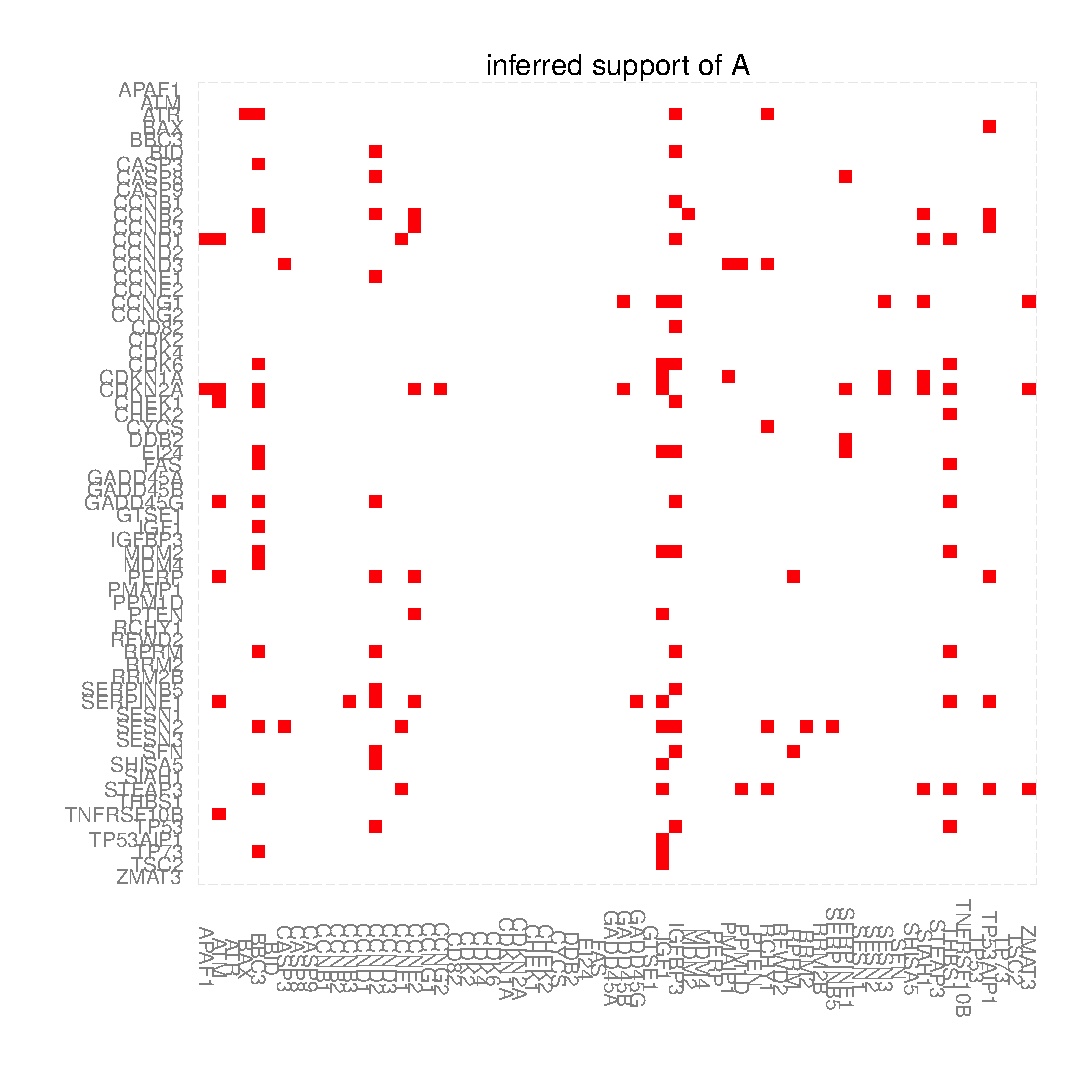
\includegraphics[scale=0.4, angle=0]{Ahat_support.eps}
&
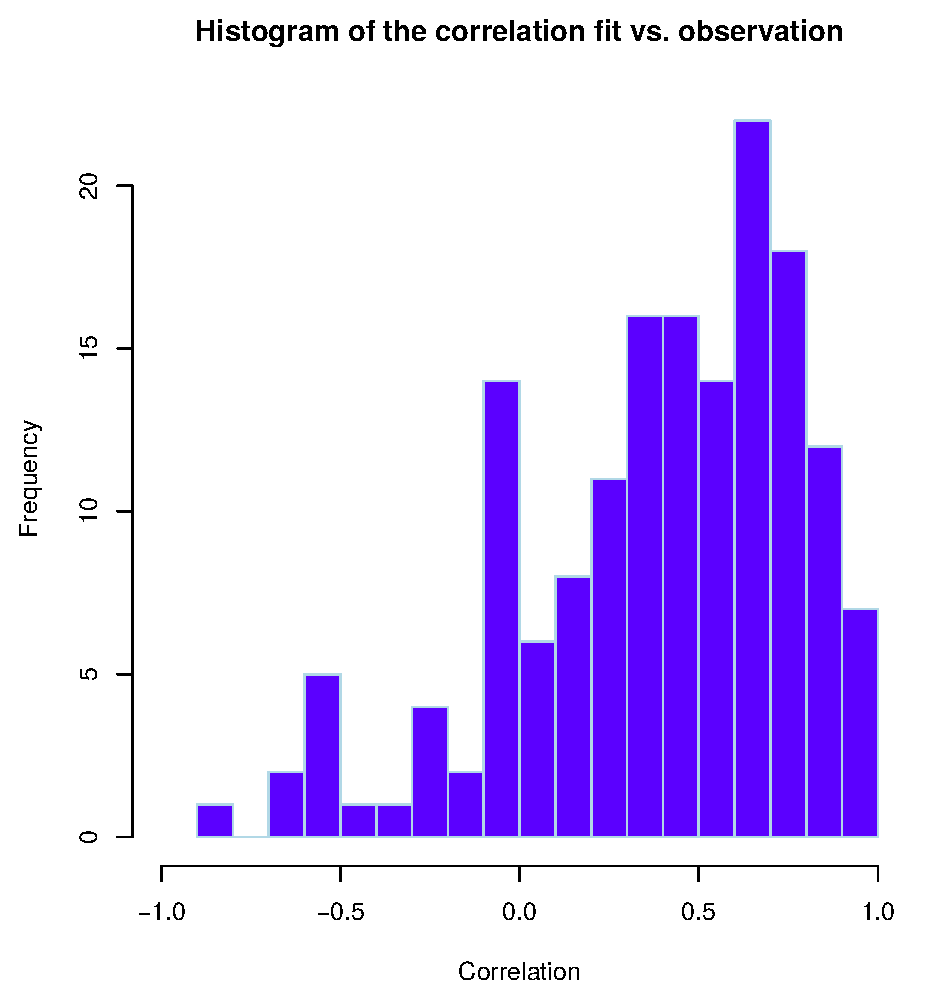
\includegraphics[scale=0.4, angle=0]{correlationFit2Obs.eps}
\\
\multicolumn{2}{c}{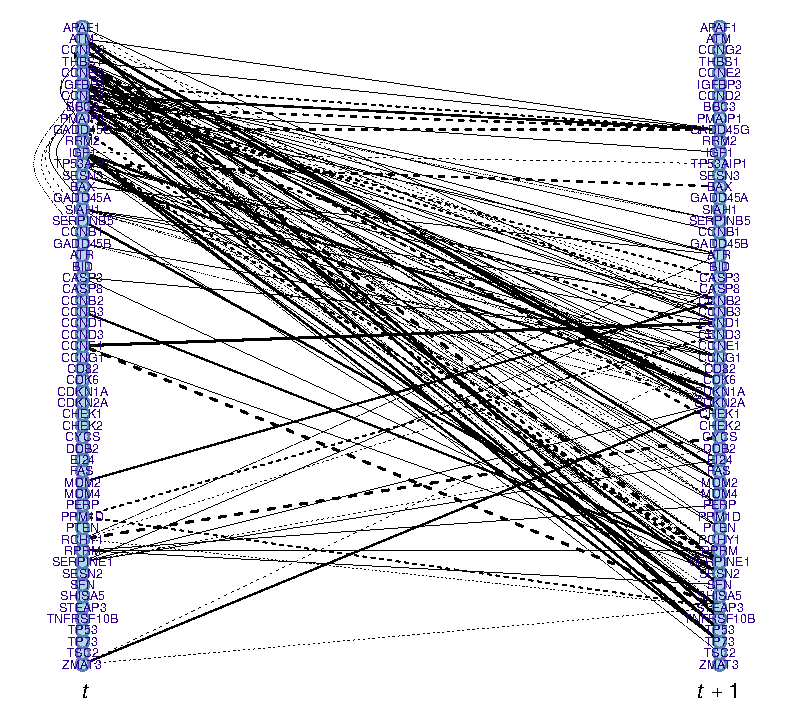
\includegraphics[scale=1.2, angle=0]{TSCG.eps}}  
\end{tabular}
\caption{Top row, left: the inferred support of $\mathbf{A}$; right: the histogram of gene-wise and cell line-wise correlation of fit and observation. Bottom panel: the time-series chain graph for the p53 signalling pathway.}
\label{fig:TSCG_supportA_fitHistogram}
\end{figure}
\afterpage{\clearpage}

The aforementioned `regulators' are known either to be pivotal to the p53 signalling pathway or to be involved in HPV-induced carcinogenesis. For instance, IGF1 (insulin-like growth factor 1) is a growth factor that regulates proliferation of both normal and cancer cells in an autocrine, paracrine \cite{Baxter2000} and potentially endocrine manner \cite{D'Ercole2001}. HPV transformed keratinocytes were found to be addicted to IGF1 signalling for survival, underlining the importance of this pathway for cervical cancer development \cite{Geiger2007}. IGFBP3, central to this signalling pathway, is transcriptionally regulated by p53 and (among others) suppresses proliferation and induces apoptosis (the process of programmed cell death). In our model lacking functional p53 due to presence of the HPV oncoprotein E6, IGFBP3 is down-regulated (data not shown) and, thus, does no longer inhibit carcinogenesis. Downregulation of THBS1, a potent angiogenesis inhibitor, was described before after expression of the viral oncogenes E6 and E7 in keratinocytes of different origins \citep{ToussaintSmith2004}. Lowered expression was also observed in cervical cancers \cite{Kodama2001}. 


With knowledge of their support less biased estimates of $\mathbf{A}$ and $\mathbf{\Omega}_{\varepsilon}$ are obtained by refitting them taking the support into account. Optimal penalty parameters are re-determined: $\lambda_a=2.55082$, $\lambda_{\omega}=0.00583$ (and confirmed by the contour plot the LOOCV log-likelihood surface, \cite{Supp2018}, Figure 3.30). Re-estimated parameters are visualized as a heatmap (\cite{Supp2018}, Figure 3.32). Using these estimates the time-series chain graph is constructed (Figure \ref{fig:TSCG_supportA_fitHistogram}). This is in line with the above suggested interpretation of `regulators'  and `regulatees'. 


Employing the re-estimated parameter $\mathbf{A}$, we study the fit ($\hat{\mathbf{Y}}_{\ast, i, t} = \hat{\mathbf{A}} \mathbf{Y}_{\ast, i, t-1}$) of the `regulatees' (genes explained by other genes). The fit is studied for all genes in the pathway. The result is summarized in Figure \ref{fig:TSCG_supportA_fitHistogram}. It displays the histogram of the Spearman correlations between the fit and the observations, cell line-wise. The histogram in Figure \ref{fig:TSCG_supportA_fitHistogram} is clearly skewed to the domain $[0,1]$. This indicates that the fit is generally reasonable. For a more tangible assessment of the fit it is displayed for several individual genes in Figure 3.34 \cite{Supp2018}.

\begin{figure}[t!]
\centering
\begin{tabular}{ccc}
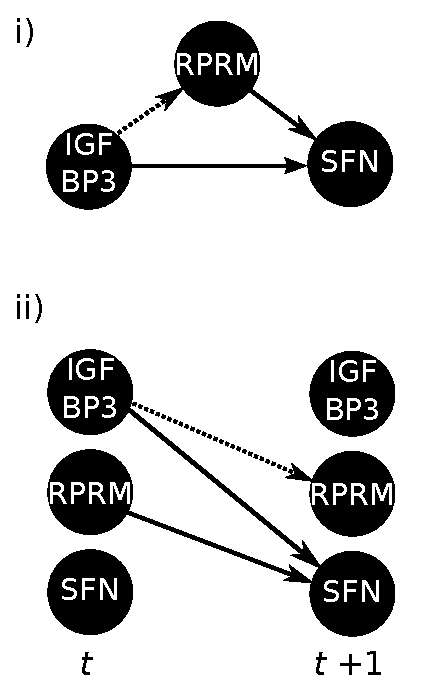
\includegraphics[scale=0.63, angle=0]{motif_incoherentFFL.eps}
& \mbox{ } \qquad \mbox{ } &
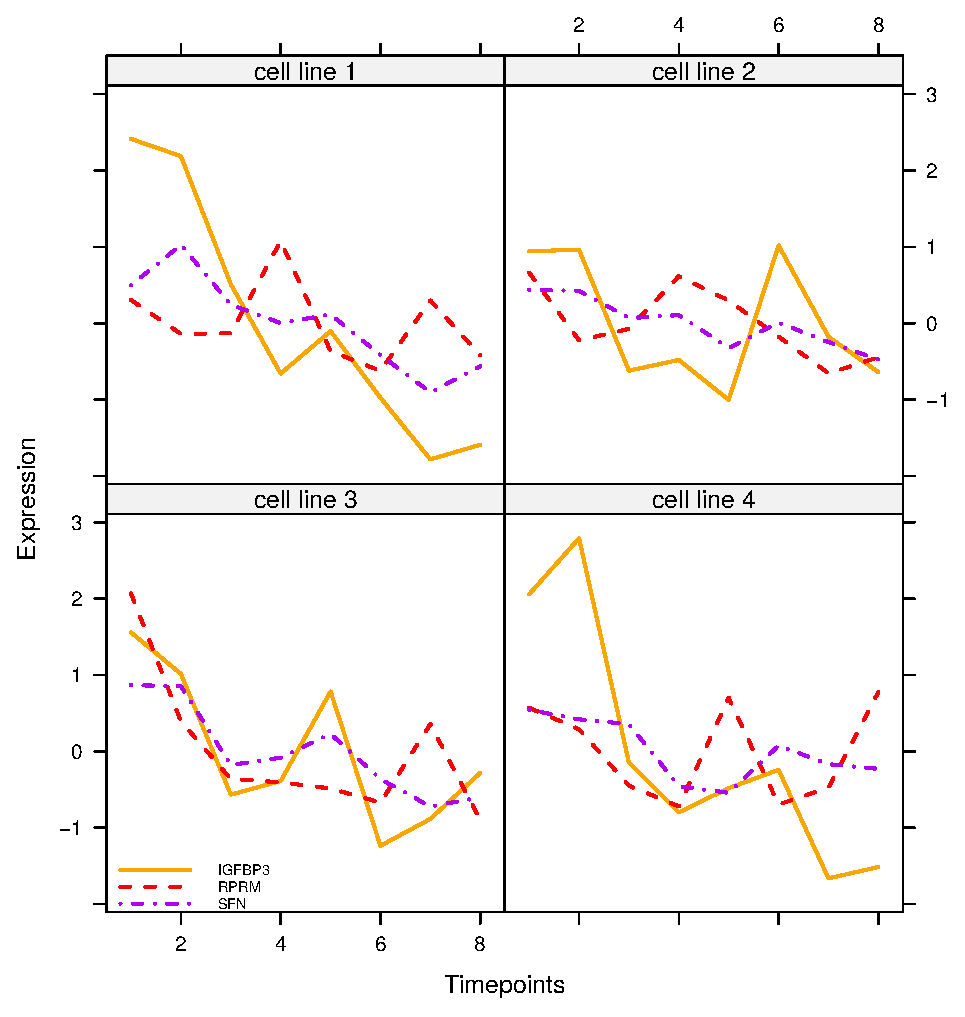
\includegraphics[scale=0.41, angle=0]{motif_incoherentFFL_data.eps}
\end{tabular}
\caption{Left panel, i): incoherent FFL motif formed by the gene-triple IGFBP3, RPRM and SFN. The solid (dashed) edge represent a positive (negative) effect. Left panel, ii): same as i) but `unrolled'. Right panel: gene expression data of the IGFBP3, RPRM and SFN genes over time in the four cell lines. }
\label{fig:motif_incoherentFFL}
\end{figure}
 \afterpage{\clearpage}


With final and less-biased estimates of the VAR(1) parameters at hand, we study the quantitative, dynamic implications of the model: what are the downstream effects of a change in expression levels of a gene? This can be done through impulse response analysis (confer Section \ref{sect:impulseResponse}). For each gene the column-wise average of the (absolute) impulse response on all other genes at the next time instance is calculated (Table 3.2, \cite{Supp2018}). This is a measure of a gene's driving force on the pathway's expression levels. The low and high impulse responses of the $\{\mbox{CCNG1, CGKN2A, SERPINE1, SESN2, STEAP3}\}$ and \\ $\{\mbox{IGF1, IGFBP3, BBC3, CCND2, THBS1}\}$ genes corroborate with their interpretations of `regulatees' and `regulators'. This is supported when evaluating the mutual information between each gene at time point $t$ and the whole pathway at the next time point (Table 3.2, \cite{Supp2018}). 

The downstream effects of a signal may be further elucidated through the decomposition of the covariance between the expression levels of two genes in terms of the paths connecting them in the time-series chain graph (as described in Section \ref{sect.pathDecomposition}). For illustration purposes consider the `regulator'-`regulatee' pair (IGF1, SESN2) at two contiguous time points. They are connected through two paths: a direct path $(Y_{\mbox{{\tiny IGF1}},t} \rightarrow Y_{\mbox{{\tiny SESN2}},t+1})$ and an indirect one through $Y_{\mbox{{\tiny IGF1}},t} \rightarrow Y_{\mbox{{\tiny RRM2}},t}\rightarrow Y_{\mbox{{\tiny SESN2}},t+1}$. The covariance of the (IGF1, SESN2) gene pair at contiguous time points may now be decomposed as: $\mbox{Cov}(Y_{\mbox{{\tiny IGF1}},t},Y_{\mbox{{\tiny SESN2}},t+1}) = (\boldsymbol{\Sigma}_{\varepsilon} \textbf{A}^\top)_{\mbox{{\tiny IGF1}}, \mbox{{\tiny SESN2}}} =  -0.05315 = -0.02203  - 0.03112$, in which the two summands on the right-hand side correspond to the direct and indirect path in the time-series chain graph. Based on the paths' contributions the indirect one dominates (surprisingly), but being of the same sign and (approximately) of the same size the direct path also contributes in the suppression of the expression levels of the SESN2 gene.


Another way to grasp the inferred networks of the p53 signalling pathway is to study its motifs. Motifs are small recurring network patterns and form the building blocks of pathways \cite{Alon2007}. It takes to far afield to study all motifs present in the inferred network (although it is relatively sparse) in depth. For the purpose of illustration we single out the feedforward loop (FFL), which appears in many gene systems \cite{Alon2007}. FFL motifs come in the coherent and incoherent variety: the latter connects two genes via two paths that have opposite effects (positive/activating and negative/repressing), while in the former both paths have the same effect. In an incohorent FFL motif found in the reconstructed time-series chain graph of the p53 signalling pathway gene IGFBP3 represses RPRM and activates SFN, while (to a lesser degree) RPRM stimulates SFN gene (Figure \ref{fig:motif_incoherentFFL}). IGFBP3 and RPRM thus affect SFN in opposite ways. In the extreme case, when the effect of the RPRM is equal to that of IGFBP3, this results (with a slight delay due to the time) in the repression of the SFN, reducing its expression levels to (virtually) zero (confer \cite{Alon2007}). In any case, the effect of IGFBP3 on SFN is moderated by that of RPRM (as is corroborated by the data (Figure \ref{fig:motif_incoherentFFL}).


\section{Conclusion}
The reconstruction of the time-series chain graph associated with a VAR(1) model from high-dimensional omics data was studied. To this end we presented a ridge penalized, full maximum likelihood estimation framework. The resulting estimator was simplified algebraically to ensure its computationally efficient evaluation from high-dimensional data. The estimator allows the incorporation of prior knowledge in two ways. First, the penalty of both VAR(1) model parameters includes a user-chosen target, representing a suggestion of the actual parameter value towards which the parameter is shrunken. Secondly, knowledge on the absence of certain cross-temporal and contemporaneous edges of the time-series chain graph may be included. Various novel ways to make use of the thus estimated  VAR(1) model were presented: \textit{i}) edge selection of the time-series chain graph from the estimated model, \textit{ii}) mutual information analysis across time points, and \textit{iii}) decomposition of the covariance between nodes across time points in terms of the paths of the time-series chain graph connecting them. Then, the proposed ridge estimation procedure was compared in simulation to a SCAD penalized estimator of the time-series chain graph. The ridge estimation procedure outperformed its SCAD counterpart in terms of loss and showed to be competitive in terms of specificity and sensitivity, in particular for small sample sizes (as is the prevalent experimental design for practice). Finally, the use of the presented methodology is illustrated on a time course experiment using an HPV-induced transformation cell line model.

Further biological questions to be (partially) answered using the high-dimensional omics data of the aforementioned cell line experiment require extensions of the proposed ridge estimation framework to more intricate vector autoregressive models. For instance, the full experiment also encompasses data from other molecular levels like DNA copy number and microRNA expression. Inclusion of these levels, both affecting mRNA expression, may be done within a VARX(1) model, a VAR(1) model with time-varying covariates (hence, the $X$ in VARX), which models the variation of mRNA expression over time by mRNA expression of the preceding time point and e.g. DNA copy number of the current time point. Another extension would address the fact that each cell line in the experiment had a different HPV inserted to initiate oncogenesis. This may lead to differences in the cell lines' time-series chain graphs. To detect such differences in regulatory architecture a VAR(1) model may be assumed per cell line and fitted with a fused ridge penalty \cite{Bilgrau2015}. Such a penalty fuses what is similar among the cell lines and preserves substantial differences among them. Future work will center around these and related topics to extract all relevant biological information from integrative time-course omics studies such as the cervical cancer one.


\chapter{Ridge estimation of network models from time-course omics data \\ {\footnotesize(\textit{Miok, V., Wilting, S. M. and van Wieringen, W. N., Under review at Biometrical Journal})}}
\chaptermark{{\tt ragt2ridges} package}
\label{chapter:Window estimator}

\graphicspath{{Chapter4/Figs/}{Chapter4/Figs/PDF/}{Chapter4/Figs/}}%

Time-course omics experiments enable the reconstruction of the dynamics of the cellular regulatory network. Here we describe the means for this reconstruction and the downstream exploitation of the inferred network. It is assumed that one of the various vector-autoregressive (VAR) models presented here serves as a reasonably accurate description of the time-course omics data. The models are estimated through ridge penalized likelihood maximization, accompanied by functionality for the determination of optimal penalty parameters. Prior knowledge on the network topology is accommodated by the estimation procedures. Various routes that translate the fitted models into more tangible implications for the medical researcher are described. The network is inferred from the -- non-sparse -- ridge estimates through empirical Bayes probabilistic thresholding. The influence of a (trait of a) molecular entity at the current time on those at future time points is assessed by mutual information, impulse response analysis, and path decomposition of the covariance. The presented methodology is applied to the omics data from the p53 signalling pathway during HPV-induced cellular transformation. All methodology is implemented in the \texttt{ragt2ridges} package, freely available from the Comprehensive {\tt R} Archive Network.
\\
\\
This chapter corresponds to the article:\\
 Miok, V., Wilting, S. M. and van Wieringen, W. N. Ridge estimation of network models from time-course omics data \textit{Under review at Biometrical Journal}.



\section{Introduction}
The cellular regulatory system processes incoming signals. The signal usually triggers the transcription of mRNAs ultimately resulting in protein complexes executing specific tasks in response to the incoming signal. The interaction pattern of the molecular entities in the cell is described by a network. This network is often learned from observational studies that interrogated multiple, independent individuals. A powerful alternative are time-course experiments. In this type of experiment cell lines are usually manipulated by either drug treatment, ectopic gene expression or knock down and subsequently interrogated at regular intervals over time. One well known example for this is the study of cellular immortalization and transformation by (viral) oncogenes, including the human papillomavirus (HPV)-encoded E6 and E7 \cite{Band1990, Durst1987, Park1991, Pecoraro1989, Pirisi1987, Willey1991}.  The resulting sequential snapshots of the activity of each molecular entity provide insight into the dynamic aspects of the regulatory system

The goal of this paper is to illustrate how and what can be learned on the regulatory network from aforementioned time-course data. The paper starts with a description of an exemplary time-course experiment, used in the illustrations, that interrogated multiple molecular levels from multiple cell lines at various time points. It is followed by an overview of the various network analyses of these data presented here, all borrowing heavily from the field of time series analysis. The methodology underlying the first analysis is fully described in \cite{Miok2017}, but recapped here as the other analyses extend it. Next, the other network analyses, each incorporating more information through a more complex model, are presented. All models are estimated by means of ridge penalized maximum likelihood. Furthermore, downstream analysis using estimated models is discussed. Each extension is applied to the exemplary time-course experiment, using the implementation offered by the \texttt{ragt2ridges} package.


\section{Experiment}
\label{sec:experiment}
Cervical cancer is one of most frequently diagnosed cancers in women worldwide, especially in developing countries \citep{Ferlay2015}. The cancer is induced by a persistent HPV infection. Of the 150 types, about 15 are known to have oncogenic potential, of which HPV16 and HPV18 together account for around 70\% of cervical cancers. Although the majority of infected women will clear the virus, a subset will develop a persistent infection that can give rise to the development of precancerous lesions which, if left untreated, can ultimately progress into an invasive carcinoma. In vitro, this process can be mimicked by transfection of human keratinocytes with oncogenic HPV types after which four consecutive phenotypic stages of the cellular transformation are recognized: expanded lifespan, immortalization, anchorage independence and finally tumorigenicity \citep{Pirisi1987}. Previous studies \citep{Steenbergen2004, Wilting2006, Henken2007} showed that the cell line experimental model faithfully mimics cervical precancerous lesions morphologically and (epi)genetically. 

We designed an experiment involving the model system described above to enhance our molecular understanding of HPV-induced carcinogenesis. The experiment comprises four cell lines, originating from the same parental cells, of which two are affected with HPV16 and two with HPV18. Previous studies \citep{Steenbergen2004, Wilting2006, Henken2007} showed that the cell line experimental model faithfully mimics cervical precancerous lesions morphologically and (epi)genetically. During continued culturing of these cell lines abnormalities arise at the molecular level of the cells. Genomic and transcriptomic characteristics of each cell line are measured at 8 different time points. At each time point their DNA copy number, mRNA and miRNA gene expression are interrogated using oligonucleotide microarrays. 

The raw data from the cell line experiment are preprocessed as follows. The DNA copy number data are median normalized and segmented using the CBS (Circular Binary Segmentation) method \citep{Olshen2004}. The mRNA gene expression data are RMA background corrected \citep{Irizarry2003}, between-array normalized by the robust quantile method \citep{Boldstad2003}, and finally transformed using a variance stabilizing transformation \citep{Huber2002}. The miRNA gene expression data are preprocessed similarly, but without the background correction. 

For the illustration of the exposed methodology and software the data are limited to that related to the p53 signaling pathway, known to be directly altered in this model system by the viral oncogene E6. The mRNA gene expression data are limited to the genes that map to the p53 signaling pathway as defined by the KEGG repository \citep{Kanehisa2000}. Based on the chromosomal location DNA copy number transcripts are matched to the mRNA expression features (employing the {\tt overlapPlus} matching procedure of the \texttt{sigaR} package, \citealp{Wieringen2012}). The miRNA transcripts are a selection on the basis of temporal differential expression (determined using the method of \citealp{Miok2014}), that are either up- or down-regulated in at least 3 out of 4 cell lines. Both mRNA gene expression and DNA copy number data then comprise $p=64$ genes, while the miRNA gene expression data  includes $q=106$ genes, all measured at $\mathcal{T}=8$ time points in $n=4$ cell lines. In the third cell line the miRNA expression hybridizations of the fourth and fifth time point failed and corresponding array columns contain missings. These (P53 signalling pathway related mRNA, miRNA, and DNA copy number) data are included in the R-package {\tt ragt2ridges}. 

\section{Methods}
Experiments like the one described above may provide insight into the temporal and contemporaneous relations among molecular entities of (say) the P53 signaling pathway. The temporal relations reflect the conditional (in)dependency between two molecular entities at consecutive time points ($t$ and $t+1$) given all others at time $t$. On the other hand, contemporaneous relations reflect the conditional in/dependency between two molecular entities at the same point given all others at the same time point \textit{and} all (!) at the preceding time point. These relations are aggregated in the time-series chain graph \citep{Dahlhaus2000}. To shed light on such graphs several multivariate statistical techniques, all based on the vector auto-regressive (VAR) processes and each answering a different question, are proposed:

\begin{compactitem}
\item The first technique aims to unravel the dynamic interrelatedness of the variates (e.g. mRNA genes) of a single molecular level (e.g. mRNA gene expression). To this end a VAR(1) model is assumed to describe the time-series data from this molecular level. The model explains the gene expression at the present time by that of the one (hence, the '1' in VAR(1) model) time point directly preceding it. The model thus explicates the temporal dependencies among the genes, but also captures the contemporaneous ones (through the inverse of the error covariance matrix). The top left panel of Figure \ref{fig:VARmodels} provides an illustration of the network of temporal and contemporaneous interactions among three genes as implicated by a VAR(1) model. 

\item The previous technique is extended to assess the presence of dynamic dependencies over a longer time range than that implied by the VAR(1) model. This is done through the VAR(2) model, which includes an additional explanatory time point, i.e. the two time points directly preceding the current one may both contribute to the observed variation in the latter. The top right panel of Figure \ref{fig:VARmodels} illustrates the temporal and contemporaneous relations among the variates captured by a VAR(2) model. 

\item When cell lines can be divided into groups (e.g. in the aforementioned experiment by the HPV type by which they have been transfected), differences among the groups' interaction networks may be identified. Hereto a group-wise VAR(1) model is assumed but fitted jointly to facilitate the borrowing of information when they share network features. The result of this approach is depicted in the right bottom panel of Figure \ref{fig:VARmodels}.



\item When information on additional molecular levels (e.g. DNA copy number or microRNA gene expression) is available, those levels may be incorporated into the network. The VARX(1) model integrates time-varying covariates from other molecular levels (corresponding the `X' in VARX) into the VAR(1) model. The network of this VAR(1) extension to include exogenous data is illustrated in bottom left panel Figure \ref{fig:VARmodels}.



\begin{figure}[h!]
\centering
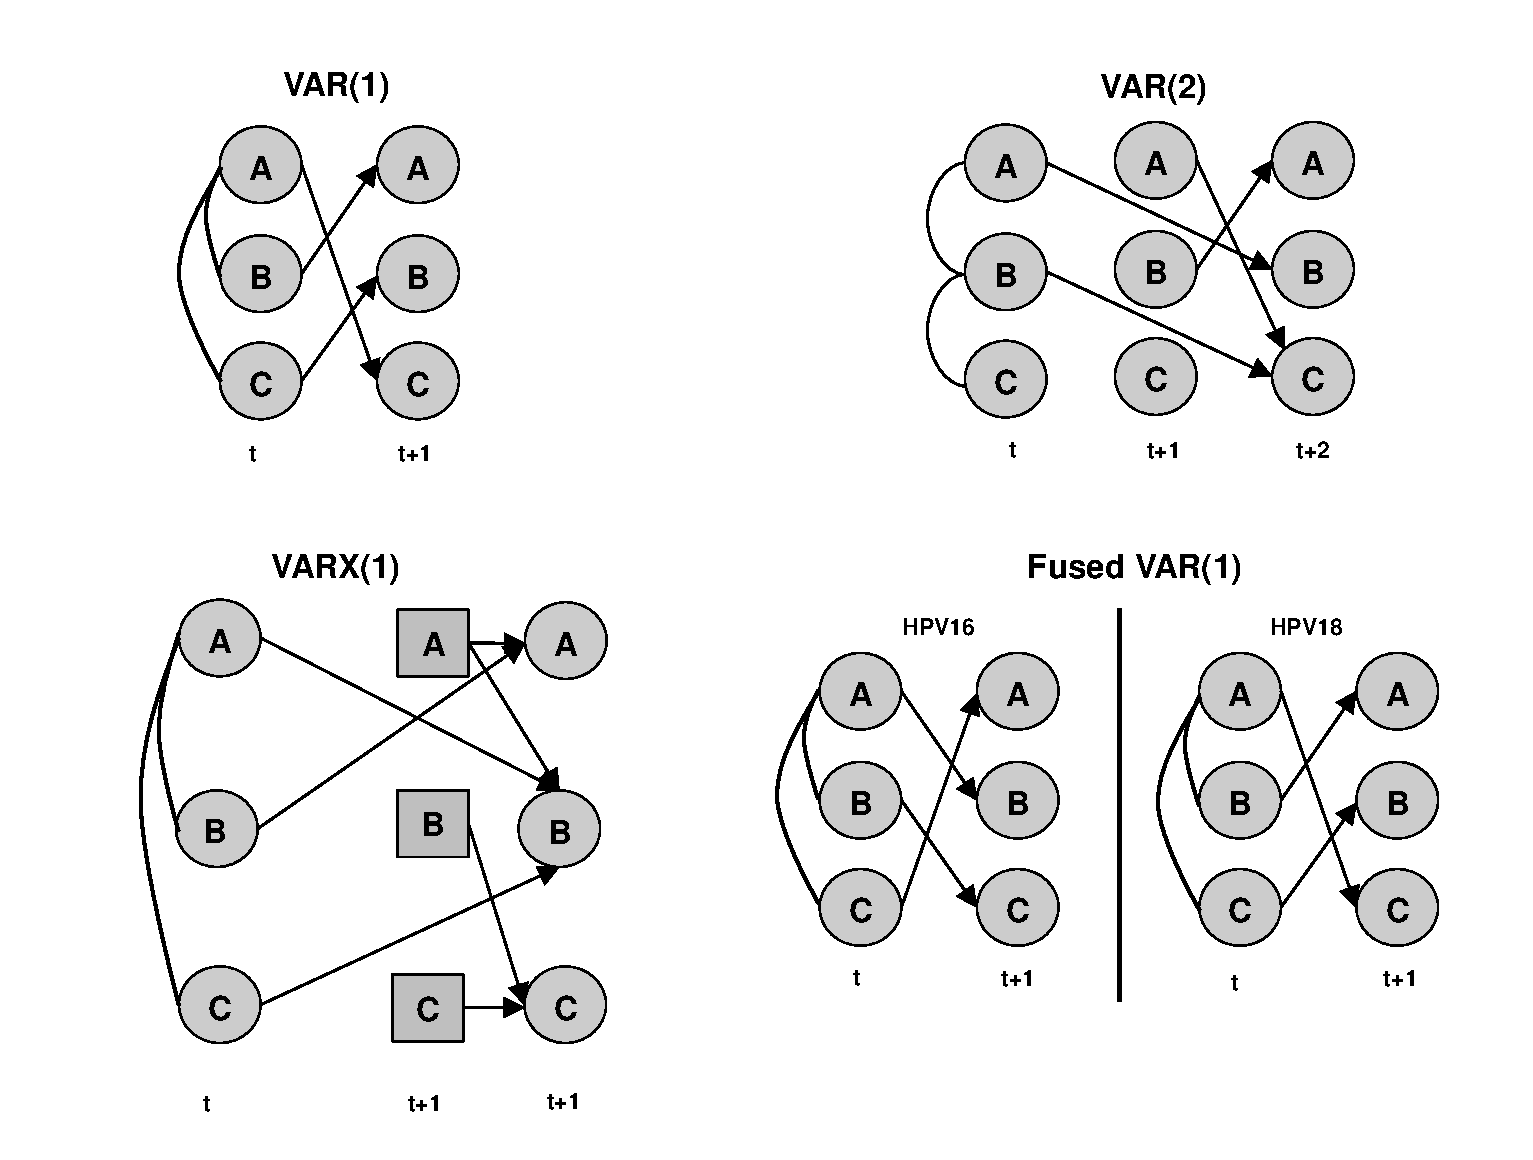
\includegraphics[scale=0.6]{Figure_2.eps}
\caption{Illustration of the time-series chain graphs underlying the various vector autoregressive models. Circles represents the endogenous molecular entities A, B and C (e.g., mRNA expression of genes) at various time points. Squares represent time-varying covariates (e.g., DNA copy number and miRNA expression). Arrows and lines indicate the temporal and contemporaneous (respectively) relations among the molecular entities. The various panels (starting top left and going clock-wise) illustrate the time-series chain graphs of the VAR(1), VAR(2), multi-group VAR(1) and VAR1(X) models.}
\label{fig:VARmodels}  
\end{figure}
\end{compactitem}
The models described above are estimated from high-dimensional data through ridge penalized, full likelihood maximization. Resulting estimates are sparsified post-estimation to arrive at a network comprising the main edges. Further methodology exploits the estimated models in order the answer additional biological questions. 



\section{The VAR(1) model}
Knowledge of the dynamic cellular regulatory patterns may enhance the understanding of cervical carcinogenesis. Hereto temporal and contemporaneous gene-gene interactions need to be identified from the HPV-cell lines data. This is facilitated by the methodology presented in \cite{Miok2017}, which also describes how inferred model and graph may be exploited to deduce tangible implications for the medical researcher. Here this is briefly recapitulated. We  refer to \cite{Miok2017} for the illustration of the VAR(1) model estimation and its down-stream exploitation on the P53 signalling pathway mRNA gene expression data of the cervical cancer time-course experiment. 


Let $\mathbf{Y}_{*,t,i}$ be a random vector representing the $p$-dimensional mRNA gene expression data of sample $i$ $(i=1,\hdots,n)$ at time point $t$ $(t=1,\hdots,\mathcal{T})$. These data are assumed to follow a VAR(1) process, where the data at the current time point $t$ are explained by that at the previous time point $t-1$. In vector form the VAR(1) model is: $\mathbf{Y}_{*,t,i}  = \boldsymbol{\nu} + \mathbf{A} \mathbf{Y}_{*,t-1,i} + \boldsymbol{\varepsilon}_{*,t,i}$, where $\boldsymbol{\nu}$ is the intercept vector assumed to be zero (i.e. $\boldsymbol{0}_{p}$), $\mathbf{A}$ is the $p \times p$-dimensional matrix of auto-regression coefficients, and $\boldsymbol{\varepsilon}_{*,t,i}$ the errors which are independently and identically distributed in accordance with a $\mathcal{N}(\boldsymbol{0}_{p}, \boldsymbol{\Omega}_{\varepsilon}^{-1})$ law. For more details about the model see \cite{Lutkepohl2005, Hamilton1994}.

Parameters of the VAR(1) model are obtained from the ridge penalized maximum likelihood (ML) estimation. The likelihood, using $\mathbf{Y}_{*,t,i}|\mathbf{Y}_{*,t-1,i}\sim\mathcal{N}(\mathbf{A}\mathbf{Y}_{*,t-1,i},\mathbf{\Omega}_{\varepsilon}^{-1})$, is $L(\mathbf{Y}; \mathbf{A}, \boldsymbol{\Omega}_{\varepsilon}) = \prod_{i=1}^n \prod_{t=2}^{\mathcal{T}}P(\mathbf{Y}_{*,t,i}|\mathbf{Y}_{*,t-1,i})$. To address the high-dimensionality of the data its logarithm is augmented with ridge penalties on the $\mathbf{A}$ and $\mathbf{\Omega}_{\varepsilon}$ parameters: $\tfrac{1}{2} \lambda_a n(\mathcal{T}-1) \| \mathbf{A} - \mathbf{A}_0 \|_F^2$ and $\tfrac{1}{2} \lambda_{\omega} n(\mathcal{T}-1) \| \mathbf{\Omega}_{\varepsilon} - \mathbf{\Omega}_0 \|_F^2$, respectively. In this $\lambda_a$ and $\lambda_{\omega}$ are penalty parameters, matrices $\mathbf{A}_0$ and $\boldsymbol{\Omega}_0$ are user-specified target matrices towards the parameters are shrunken for large values of the penalty parameters, and $\| \cdot \|_F$ denotes the Frobenius norm. 


The estimators of the VAR(1) model parameters $\mathbf{A}$ and $\boldsymbol{\Omega}_{\varepsilon}$ are obtained through ridge penalized log-likelihood maximization (see \cite{Miok2017} for details). The estimator of autoregression parameters $\mathbf{A}$ (fixing $\boldsymbol{\Omega}_{\varepsilon}$) is: 
\begin{eqnarray}\label{ridgeA1}
\mbox{vec}[ \hat{\mathbf{A}}(\lambda_a) ] & = &  [\lambda_a \mathbf{I}_{p^2 \times p^2}  + \hat{\boldsymbol{\Gamma}}(0) \otimes \mathbf{\Omega}_{\varepsilon} \big) ]^{-1} \times \, \{ \lambda_a \mbox{vec}(\mathbf{A}_0) + \mbox{vec} [\mathbf{\Omega}_{\varepsilon} \hat{\boldsymbol{\Gamma}}(-1) ] \},
\end{eqnarray}
where $\hat{\boldsymbol{\Gamma}}(0) = \frac{1}{n(\mathcal{T}-1)} \sum_{i=1}^{n}\sum_{t=2}^{\mathcal{T}} \mathbf{Y}_{*,t-1,i} \mathbf{Y}_{*,t-1,i}^{\top}$ and \\
$\hat{\boldsymbol{\Gamma}}(-1) = \frac{1}{n(\mathcal{T}-1)} \sum_{i=1}^{n} \sum_{t=2}^{\mathcal{T}} \mathbf{Y}_{*,t,i} \mathbf{Y}_{*,t-1,i}^{\top}$. The error precision matrix estimator, for fixed $\mathbf{A}$, is (cf. \cite{Wieringen2016}): 
\begin{eqnarray} \label{ridgePrecision}
\widehat{\mathbf{\Omega}}_{\varepsilon} (\lambda_{\omega}) & = & \{ [ \lambda_{\omega} \mathbf{I}_{p \times p} + \tfrac{1}{4} (\mathbf{S}_{\varepsilon} - \lambda_{\omega} \mathbf{\Omega}_0)^2 ]^{1/2} +
\tfrac{1}{2} (\mathbf{S}_{\varepsilon} - \lambda_{\omega} \mathbf{\Omega}_0) \}^{-1},
\end{eqnarray}
where $\mathbf{S}_{\varepsilon}$ is the sample covariance matrix of the errors:
\begin{eqnarray*}
\mathbf{S}_{\varepsilon} & = & \frac{1}{n(\mathcal{T}-2)}\sum_{i=1}^{n} \sum_{t=2}^{\mathcal{T}} \left[\mathbf{Y}_{*,t,i} - \mathbf{A} \mathbf{Y}_{*,t-1,i} \right] \left[\mathbf{Y}_{*,t,i} - \mathbf{A} \mathbf{Y}_{*,t-1,i} \right]^{\top}.
\end{eqnarray*}
The final estimators of $\mathbf{A}$ and $\boldsymbol{\Omega}_{\varepsilon}$ result from an iterative procedure which alternates between the updating of one estimator while keeping the other fixed, until convergence. The procedure is initiated with the ridge least squares estimator of $\mathbf{A}$, which does not involve $\boldsymbol{\Omega}_{\varepsilon}$. In this penalty parameters $\lambda_a$ and $\lambda_{\omega}$ are chosen to maximize the leave-one-out cross-validated (LOOCV) log-likelihood. 

Prior to the parameter estimation, the penalty parameters $\lambda_a$ and $\lambda_{\omega}$ are chosen through LOOCV log-likelihood maximization. The convergence of this optimization procedure may be inspected visually by contourplots. With optimal penalty parameters at hand, the (penalized) estimates of $\mathbf{A}$ and $\boldsymbol{\Omega}_{\varepsilon}$ are obtained. 

The resulting ridge estimates of $\mathbf{A}$ and $\mathbf{\Omega}_{\varepsilon}$ are not sparse. For many practical purposes, however, this is desirable. To this end their support may be inferred  by means of various  post-estimation thresholding procedures. Minimally sophisticated choices would be: \textit{1)} thresholding on the absolute values of the matrix entries, and \textit{2)} selection of the top absolute values of $\mathbf{A}$. A third procedure with a more probabilistic flavour employs the empirical Bayes approach of \cite{Efron2004} and implemented by \cite{Strimmer2008}), which yields the probability of an edge being ``interesting'' given its observed edge strength (i.e., a statistic derived from the parameter estimates, cf. \cite{Miok2017}, Section 4).
 
The inferred support does not -- strictly -- match with the non-sparse parameter estimates. To align those two the VAR(1) model is re-fitted. To this end penalty parameters need to be re-determined, now accommodating the inferred support of the VAR(1) model parameters. As the optimal penalty parameters are likely to be smaller, this will yield less biased estimates. With re-determined penalty parameters the final estimate of the VAR(1) model parameters are obtained. The final VAR(1) model is visualized as a time-series chain graph depicting all temporal and contemporaneous relations (see Figure 1 of \cite{Miok2017}).

To facilitate the understanding of the (mRNA expression) dynamics implied by the fitted VAR(1) model \citep{Miok2017} present several downstream analyses. A first step in this direction is impulse response analysis, which evaluates the effect of a change in the error at one time point on the variates at a future time point. For the VAR(1) model this change, operationalized as the derivative of $Y_{*, i, t+\tau}$ with respect to $\varepsilon_{*, i, t}$, amounts to $\mathbf{A}^{\tau}$ \citep{Hamilton1994}. This may be helpful when designing knock-out experiments. Alternatively, mutual information analysis yields a (generalized) correlation measure between the variate at one time point and the variates at a future time point. The mutual information of the VAR(1) model is:
\begin{eqnarray*}
\mathcal{I}(\mathbf{Y}_{*,t+\tau,i},Y_{j,t,i}|\mathbf{Y}_{*,t-1,i},\mathbf{Y}_{*,t-2,i}) & = & \log \{ |\mbox{Var}(\mathbf{Y}_{*,t+\tau,i}|\mathbf{Y}_{*,t-1,i},\mathbf{Y}_{*,t-2,i}) | \}-  
\\
& & \log \{ | \mbox{Var}(\mathbf{Y}_{*,t+\tau,i}|Y_{j,t,i},\mathbf{Y}_{*,t-1,i},\mathbf{Y}_{*,t-2,i}) | \}.
\end{eqnarray*}
This measure aids in the identification of the most influential nodes.


With re-estimated model parameters and the inferred network at hand, node statistics can be calculated: various network measures, e.g. degree, centrality (see \cite{Newman2010}), mutual information, and impulse response. Table 1 of \cite{Miok2017} presents these for the most interesting genes from the P53 signaling pathway model, defined by a large number of out- and in-degree edges and, henceforth, for convenience referred to as `regulators' and `regulatees' genes, respectively. For these genes centrality measures, mutual information and impulse response are given. The centrality measures are indeed high for `regulators', which corroborates with it intuitively understood by an influential node.

Finally, path decomposition analysis unravels the association between two nodes at different time points in terms of the paths connecting them. Hereto the covariance between $Y_{j_1,t,i}$ and $Y_{j_2,t+\tau,i}$ for $\tau\ge 0$ can be decomposed as a sum over all paths connecting $j_1$ and $j_2$ in the time-series chain graph \citep{Miok2017}:
\begin{eqnarray*}
\mbox{Cov}(Y_{j_1,t,i},Y_{j_2,t+\tau,i}|\mathbf{Y}_{*,t-1,i}) \, \, \, = \, \, \, (\mathbf{\Sigma}_{\varepsilon} \mathbf{A}^{\tau})_{j_1,j_2}\, \, \, = \, \, \,\sum_{j'=1}^p (\mathbf{\Sigma}_{\varepsilon})_{j_1,j'} (\mathbf{A}^{\tau})_{j',j_2},
\end{eqnarray*}
where $(\mathbf{\Sigma}_{\varepsilon})_{j_1,j'}$ can be further decomposed in terms of the contemporaneous paths connecting $j_1$ and $j'$ (see \cite{Jones2005}). As such it guides in the search for the most important paths by which a molecular signal travels between these two nodes. 


\section{The VAR(2) model}
The VAR(1) model uses only information of the last time point to explain that of the next. The dynamics may, however, extend over more than two time points. That is, an additional explanatory time point may yield a significantly better fit. This can be assessed using a VAR(2) model, which includes an extra historical time point to explain the variation in the present. The VAR(2) model, where the `2' again refers to the lag in the explanatory part of the model, is:
\begin{eqnarray*}
\mathbf{Y}_{*,t,i}  & = & \boldsymbol{\nu} + \mathbf{A}_1 \mathbf{Y}_{*,t-1,i} + \mathbf{A}_2 \mathbf{Y}_{*,t-2,i} + \boldsymbol{\varepsilon}_{*,t,i},
\end{eqnarray*}
in which $\mathbf{Y}_{*,t,i}$, $\boldsymbol{\nu}$ and $\boldsymbol{\varepsilon}_{*,t,i}$, endowed with an identical and independent normal distributional assumption: $\boldsymbol{\varepsilon}_{*,t,i} \sim \mathcal{N}( \mathbf{0}_{p}, \mathbf{\Sigma}_{\varepsilon})$ (as for the VAR(1) model). The parameters $\mathbf{A}_1$ and $\mathbf{A}_2$ are the lag one and two auto-regression coefficient matrices, respectively. Finally, as for the VAR(1) model, we assume that (after centering) $\boldsymbol{\nu} = \mathbf{0}_{p}$. The VAR(2) model is often rewritten in the form of a VAR(1) model:
\begin{eqnarray} \label{form:VAR2asVAR1}
\left(\begin{array}{l} \mathbf{Y}_{*,t,i} \\ \mathbf{Y}_{*,t-1,i}  \end{array} \right) & = & \left( \begin{array}{ll} \mathbf{A}_1 & \mathbf{A}_2 \\ \mathbf{I}_{pp} & \mathbf{0}_{pp} \end{array} \right) \left( \begin{array}{l} \mathbf{Y}_{*,t-1,i} \\ \mathbf{Y}_{*,t-2,i}  \end{array} \right) + \left( \begin{array}{l}  \boldsymbol{\varepsilon}_{*,t,i}
\\ \mathbf{0}_{p} \end{array} \right).
\end{eqnarray}
More condensed, this amounts to $\mathbf{Z}_{*,t,i}  =  \mathbf{C} \mathbf{Z}_{*,t-1,i} +  \tilde{\boldsymbol{\varepsilon}}_{*,t,i}$, 
with definitions of its constituents straightforwardly deduceable from Equation (\ref{form:VAR2asVAR1}). The error precision matrix of the rewritten model, denoted $\tilde{\mathbf{\Omega}}_{\varepsilon}$, is a $2\times 2$ block matrix matrix with the left upper block equal to $\mathbf{\Sigma}_{\varepsilon}^{-1}$ with the other blocks all equalling $\mathbf{0}_{p \times p}$. This precision matrix is degenerated -- as it is not strictly positive definite -- but is defined here only for the derivation of the parameter estimators.

The parameters of the VAR(2) model are estimated by means of a ridge ML procedure. Using the Markov property implied by the VAR(2) model, the likelihood is:
\begin{eqnarray*}
L(\mathbf{Y}; \mathbf{A}_1, \mathbf{A}_2, \boldsymbol{\Sigma}_{\varepsilon}) & = & \prod_{i=1}^n \prod_{t=3}^{\mathcal{T}}P(\mathbf{Y}_{*,t,i}|\mathbf{Y}_{*,t-1,i},\mathbf{Y}_{*,t-2,i}).
\end{eqnarray*}
The normal assumption on the error enables the likelihood to be expressed explicitly in terms of the VAR(2) model parameters. Take the logarithm and augment the result with the ridge penalty $\lambda_{a,1} \| \mathbf{A}_1 - \mathbf{A}_{1,0} \|_2^2 + \lambda_{a,2} \| \mathbf{A}_2 - \mathbf{A}_{2,0} \|_2^2 + \lambda_{\omega} \| \mathbf{\Omega}_{\varepsilon} - \mathbf{\Omega}_{0} \|_2^2$. The first two summands of the penalty are written as $\mbox{tr}\{ [ \mbox{vec}(\mathbf{C}) - \mbox{vec}(\mathbf{C}_0)]^{\top} \mathbf{\Lambda}_a [ \mbox{vec}(\mathbf{C}) - \mbox{vec}(\mathbf{C}_0)] \}$ in which $\mathbf{\Lambda}_a$ a $4p^2 \times 4p^2$ dimensional, diagonal matrix with $(\mathbf{\Lambda}_a)_{jj} = \lambda_{a,1}$ for $j=1,\ldots, 2p^2$ and $(\mathbf{\Lambda}_a)_{jj} = \lambda_{a,2}$ for $j=2p^2 +1,\ldots, 4p^2$. This gives the penalized log-likelihood. To obtain the estimator of $\mathbf{C}$ (and thereby $\mathbf{A}_1$ and $\mathbf{A}_2$), equate the derivative of the penalized log-likelihood with respect to $\mathbf{C}$ to zero. Solving the resulting estimating equation gives the ridge ML estimator:
\begin{eqnarray*}
\textrm{vec} \big[\widehat{\mathbf{C}}(\boldsymbol{\Lambda}_a) \big] & = & \big[\boldsymbol{\Lambda}_a + \widehat{\boldsymbol{\Gamma}}_{zz}(0) \otimes\tilde{\boldsymbol{\Omega}}_{\varepsilon} \big]^{-1}
\big\{ \boldsymbol{\Lambda}_a \textrm{vec}(\mathbf{C}_0)+\textrm{vec} \big[ \tilde{\boldsymbol{\Omega}}_{\varepsilon} \widehat{\boldsymbol{\Gamma}}_{zz}(-1)\big] \big\},
\end{eqnarray*}
where $\widehat{\boldsymbol{\Gamma}}_{zz} (0) = \frac{1}{n(\mathcal{T}-2)} \sum_{i=1}^{n} \sum_{t=3}^{\mathcal{T}} \mathbf{Z}_{*,t-1,i} \mathbf{Z}_{*,t-1,i}^{\top}$ and \\
 $\widehat{\boldsymbol{\Gamma}}_{zz}(-1) = \frac{1}{n (\mathcal{T}-2) } \sum_{i=1}^{n} \sum_{t=3}^{\mathcal{T}} \mathbf{Z}_{*,t,i}\mathbf{Z}_{*,t-1,i}^{\top}$. 

To ensure that the bottom left and right $p \times p$ dimensional blocks of the matrix $\mathbf{C}$ are indeed $\mathbf{I}_{pp}$ and $\mathbf{0}_{pp}$ we impose linear equality constraints on corresponding elements of $\mathbf{C}$. Let the linear equality constraints on $\mathbf{C}$ be given by $\mathbf{Q} \textrm{vec}(\mathbf{C})=\mathbf{d}$, where $\mathbf{Q}$ and $\mathbf{d}$ are $(2p^2+q)\times 4p^2$ and $(2p^2+q)\times 1$ dimensional matrices with $q$ the number of additional equality constraints on the $\mathbf{A}_1$ and $\mathbf{A}_2$ implied by their support. The ridge ML estimator subject to these equality constraints, denoted $\mbox{vec}[ \widehat{\mathbf{C}}_c(\boldsymbol{\Lambda}_c) ]$, is then (cf. \cite{Miok2017}):
\begin{eqnarray*}
\mbox{vec}[ \widehat{\mathbf{C}}_c(\boldsymbol{\Lambda}_c) ] & = & \mbox{vec}[ \widehat{\mathbf{C}}(\boldsymbol{\Lambda}_c) ] - [ \boldsymbol{\Lambda}_c+\hat{\boldsymbol{\Gamma}}(0) \otimes \tilde{\boldsymbol{\Omega}}_{\varepsilon} ]^{-1}
\\
& & \qquad \times \mathbf{Q}^{\top} \big\{ \mathbf{Q} \big[ \mathbf{\Lambda}_c + \hat{\boldsymbol{\Gamma}}(0) \otimes \tilde{\boldsymbol{\Omega}}_{\varepsilon} \big]^{-1} \mathbf{Q}^{\top} \big\}^{-1} \big\{ \mathbf{Q} \textrm{vec}[ \widehat{\mathbf{C}}_c(\boldsymbol{\Lambda})]-\mathbf{d} \big\},
\end{eqnarray*}
where $\mbox{vec}[ \hat{\mathbf{C}}(\boldsymbol{\Lambda}_c) ]$ is the unconstrained ridge ML estimate.

The Kronecker product in the estimator of $\mathbf{C}$ (containing the VAR(2) auto-regression parameters $\mathbf{A}_1$ and $\mathbf{A}_2$) obstructs its evaluation for relatively small $p$ (as it is of dimensions $p^2 \times p^2$). In case of the VAR(1) model such large matrices were avoided through the rewriting of the estimator to an analytic expression involving only matrices of dimensions $p \times p$. The same derivation cannot be applied here due to the use of different penalty parameter $\lambda_{a,1}$ and $\lambda_{a,2}$ for the two auto-regression parameters $\mathbf{A}_1$ and $\mathbf{A}_2$. More specifically, $\lambda_{a,1} \not = \lambda_{a,2}$, the inverse in the estimator cannot be simplified (through the eigendecomposition of the Kronecker product $\lambda \mathbf{I}_{p^2 \times p^2 } + \mathbf{A} \otimes \mathbf{B} = (\mathbf{V}_a \otimes \mathbf{V}_{b}) (\lambda \mathbf{I}_{p^2 \times p^2}  +  \mathbf{D}_a \otimes \mathbf{D}_{b}) (\mathbf{V}_a^{\top} \otimes \mathbf{V}_{b}^{\top})$ with the matrices $\mathbf{V}$ and $\mathbf{D}$ containing the eigenvectors and -values of the corresponding matrix) in terms lower dimensional matrices. However, this inverse can be approximated by $2p \times 2p$ dimensional matrices. For the approximation, write $\nu_1 = {\textstyle\frac{1}{2}} (\lambda_{a,1} + \lambda_{a,2})$ and $\nu_2 = {\textstyle\frac{1}{2}} (\lambda_{a,1} - \lambda_{a,2})$. Then:
%\begin{eqnarray*}
\begin{flalign*}
[\boldsymbol{\Lambda}_a + \tilde{\boldsymbol{\Gamma}}_{ZZ}(0) \otimes \boldsymbol{\Omega}_{\varepsilon}]^{-1} & = & \left[ \nu_1 \mathbf{I}_{4p^2 \times 4p^2} + \nu_2
\left(
\begin{array}{rr}
\mathbf{I}_{2p^2 \times 2p^2} & \mathbf{0}_{2p^2 \times 2p^2}
\\
\mathbf{0}_{2p^2 \times 2p^2} & - \mathbf{I}_{2p^2 \times 2p^2}
\end{array}
\right) + \tilde{\boldsymbol{\Gamma}}_{ZZ}(0) \otimes \tilde{\boldsymbol{\Omega}}_{\varepsilon} \right]^{-1} 
\\
& \approx & \mathbf{\Theta}^{-1} - \nu_2 \mathbf{\Theta}^{-1} \left(
\begin{array}{cc} \mathbf{I}_{2p^2 \times 2p^2} & \mathbf{0}_{2p^2 \times 2p^2}
\\
\mathbf{0}_{2p^2 \times 2p^2} & - \mathbf{I}_{2p^2 \times 2p^2}
\end{array}
\right) \mathbf{\Theta}^{-1} \qquad \qquad \qquad  \quad
\\
& = & \mathbf{\Theta}^{-1} - \nu_2 \mathbf{\Theta}^{-2}  + 2 \nu_2 \mathbf{\Theta}^{-1} \left(
\begin{array}{cc} \mathbf{0}_{2p^2 \times 2p^2} & \mathbf{0}_{2p^2 \times 2p^2}
\\
\mathbf{0}_{2p^2 \times 2p^2} & - \mathbf{I}_{2p^2 \times 2p^2}
\end{array} \right) \mathbf{\Theta}^{-1}, \qquad
%\end{eqnarray*}
\end{flalign*}

where $\mathbf{\Theta} =  \nu_1 \mathbf{I}_{4p^2 \times 4p^2} + \tilde{\boldsymbol{\Gamma}}_{ZZ}(0) \otimes \tilde{\boldsymbol{\Omega}}_{\varepsilon}$. The eigen-decomposition can readily be applied to the first two terms in the approximation. But also to the last as only a subset of the eigenvectors shares the same nonzero eigenvalue.

For the ridge ML estimation of the non-null block of the error precision $\tilde{\boldsymbol{\Omega}}_{\varepsilon}$, the sample covariance of the innovations of the VAR(2) model is
%\begin{eqnarray*}
\begin{flalign*}
\resizebox{1.05\hsize}{!}{$
\mathbf{S}_{\varepsilon} = \frac{1}{n(\mathcal{T}-2)}\sum_{i=1}^{n} \sum_{t=3}^{\mathcal{T}} \left[\mathbf{Y}_{*,t,i} - \mathbf{A}_1 \mathbf{Y}_{*,t-1,i} - \mathbf{A}_2 \mathbf{Y}_{*,t-2,i} \right] \left[\mathbf{Y}_{*,t,i} - \mathbf{A}_1 \mathbf{Y}_{*,t-1,i} - \mathbf{A}_2 \mathbf{Y}_{*,t-2,i} \right]^{\top}. \qquad
$}
%\end{eqnarray*}
\end{flalign*}
The estimator of non-null block of $\tilde{\boldsymbol{\Omega}}_{\varepsilon}$ is then as before but with the above defined $\mathbf{S}_{\varepsilon}$ substituted.

The estimators of the $\mathbf{C}$ (and thereby $\mathbf{A}_1$ and $\mathbf{A}_2$) and the non-null block of $\tilde{\boldsymbol{\Omega}}_{\varepsilon}$ are now combined in an iterative procedure alternating between the estimation of one given the other and their roles reversed in the next step. The iterative procedure is initiated with the ridge LS estimator of $\mathbf{C}$ given by:
\begin{eqnarray*}
\widehat{\mathbf{C}}(\Lambda_a) & = & \big\{ \boldsymbol{\Lambda}_a \textrm{vec}(\mathbf{C}_0) + \textrm{vec}[\tilde{\boldsymbol{\Gamma}}(-1)] \big\} \big[\boldsymbol{\Lambda}_c + \tilde{\boldsymbol{\Gamma}}(0)\otimes \mathbf{I}_{2p\times2p} \big]^{-1},
\end{eqnarray*}
which may be obtained from the ridge ML estimator of $\mathbf{C}$ with $\mathbf{\Omega}_{\varepsilon} = \mathbf{I}_{p \times p}$. Penalty parameters $\lambda_{a_1}$, $\lambda_{a_2}$ and $\lambda_{\omega}$ are chosen to  maximize the leave-one-out cross-validated log-likelihood.

The use of the VAR(2) model and its estimation is illustrated on the mRNA expression data of the experiment described in Section \ref{sec:experiment}. First, optimal penalty parameters are determined by means of LOOCV: $\lambda_{a_{1}}=0.0398$, $\lambda_{a_{2}}=13.0090$ and $\lambda_{\omega}= 0.0068$. Their optimality is verified visually employing contourplots (cf. Figure 4.1, \cite{Supp2018}). With these optimal penalty parameters the autoregression coefficient matrices $\mathbf{A}_1$ and $\mathbf{A}_2$ as well as the precision matrix $\boldsymbol{\Omega}_{\varepsilon}$ are estimated.

For the reconstruction of the time-series chain graph the support of the matrices $\mathbf{A}_1$, $\mathbf{A}_2$ and the non-null block  of $\tilde{\mathbf{\Omega}}_{\varepsilon}$ needs to be inferred. Sparsification proceeds as for the VAR(1) model (see \cite{Miok2017}, Section 4). In the application to the HPV-cell line data a cut-off level of $1-\widehat{\ell FDR} \le 0.95$  is used in the sparsification. With the thus gained knowledge on the zero elements final, less biased estimates of $\mathbf{A}_1$, $\mathbf{A}_2$ and $\tilde{\mathbf{\Omega}}_{\varepsilon}$ are obtained using re-optimized penalty parameters: $\lambda_{a_{1}}=0.3310$, $\lambda_{a_{2}}=2.0324$ and $\lambda_{\omega}= 0.0063$. These are checked using contour plots (cf. Figure 4.1, \citep{Supp2018}). The temporal and contemporaneous relations of the final VAR(2) model may be depicted as a time-series chain graph (see Figure 4.2, \cite{Supp2018}).

As for the VAR(1) model impulse response analysis of the VAR(2) model determines the effect of a change in an innovation $\varepsilon_{j,t,i}$ at one time point on a variate $Y_{j_2,t+\tau, i}$ ($\tau \in \mathbb{N}$) at some later time point. In case of the VAR(2) model no analytic expression for the derivative of the variate with respect to the innovation exists. However, it can be expressed by a simple recursive relation:
\begin{eqnarray*}
\frac{\partial \mathbf{Y}_{*,t+\tau,i}}{\partial \boldsymbol{\varepsilon}_{*,t,i}} & = & \mathbf{A}_1 \frac{\partial \mathbf{Y}_{\ast, t+\tau-1, i} }{\partial\boldsymbol{\varepsilon}_{\ast,t,i}} +  \mathbf{A}_2 \frac{\partial  \mathbf{Y}_{\ast, t+\tau-2, i} }{\partial\boldsymbol{\varepsilon}_{\ast,t,i}} \qquad \mbox{for } \tau \geq 2.
\end{eqnarray*}
The recursive relation is initiated when noting that $\partial \mathbf{Y}_{t} \slash \partial \boldsymbol{\varepsilon}_{t} =  \mathbf{I}_{pp}$ for $\tau = 0$ and $\partial \mathbf{Y}_{t+1} \slash \partial \boldsymbol{\varepsilon}_{t} = \mathbf{A}_1$ for $\tau = 1$. In addition to the impulse response analysis, we calculate the mutual information between $Y_{j,t,i}$ and $\mathbf{Y}_{\ast,t+\tau,i}$ (given $\mathbf{Y}_{*,t-\tau,i}$ for $\tau \in \mathbb{N}$). It is defined as:
\begin{eqnarray*}
& & \hspace{-1cm} \mathcal{I}(\mathbf{Y}_{\ast,t+\tau,i},Y_{j,t,i}|\mathbf{Y}_{*,t-1,i},\mathbf{Y}_{*,t-2,i}) \, \, \, = \, \, \,
\\
& & \mathcal{H}(\mathbf{Y}_{*,t+\tau,i} \, | \, \mathbf{Y}_{*,t-1,i},\mathbf{Y}_{*,t-2,i}) - \mathcal{H}(\mathbf{Y}_{*,t+\tau,i} \, | \, Y_{j,t,i},\mathbf{Y}_{*,t-1,i},\mathbf{Y}_{*,t-2,i}),
\end{eqnarray*}
where $\mathcal{H}(\cdot|\cdot)$ is the (conditional) entropy. Under normality this the logarithm of the generalized variance (i.e. the determinant of the variance matrix). For the VAR(2) model this variance is specified through a recursive relationship (detailed in Section 4.1, \cite{Supp2018}). These variate-wise network statistics are calculated and shown in Figure 4.1, \cite{Supp2018}.


The value of an additional explanatory time point may now be assessed by comparing the fit of the VAR(1) and VAR(2) models. To this end the cell line-wise Spearman correlation between fitted and observed values of each variate/gene is calculated. The histograms of these correlation for both models are shown in Figure \ref{fig:compVAR1-2} (left panels). Both histograms reveal a similar right-skewed distribution. Indeed, a QQ-plot (right panel of Figure \ref{fig:compVAR1-2}) shows rather similar distributions. In this it should be noted that, due to the sparsified fit, the correlation for the variates without incoming edges cannot be evaluated (and are thus not included in the histogram). As a consequence more correlations are included in the histogram of the VAR(2) model due to due to fact that more nodes have an incoming edges as edges may result from either $\mathbf{A}_1$ and/or $\mathbf{A}_2$. This is reflected in the number of non-zero elements: the matrix $\mathbf{A}$ of the VAR(1) model contains 134 nonzero elements, while the matrices $\mathbf{A}_1$ and $\mathbf{A}_2$ of the VAR(2) model have 107 and 138 non-zero elements, respectively. Finally, note that these correlations with the VAR(1) and VAR(2) fit are calculated using 7 and 6 time points, respectively, due to the difference in lag. Overall, withstanding the last caveat, we are led to conclude from the qq-plot that the data do not provide enough evidence to prefer the more complicated VAR(2) model over the VAR(1) model.


\begin{figure}[h!]
\centering
\begin{tabular}{ccc}
\includegraphics[scale=0.275]{Figure_7a.eps} & 
\includegraphics[scale=0.275]{Figure_7b.eps} &
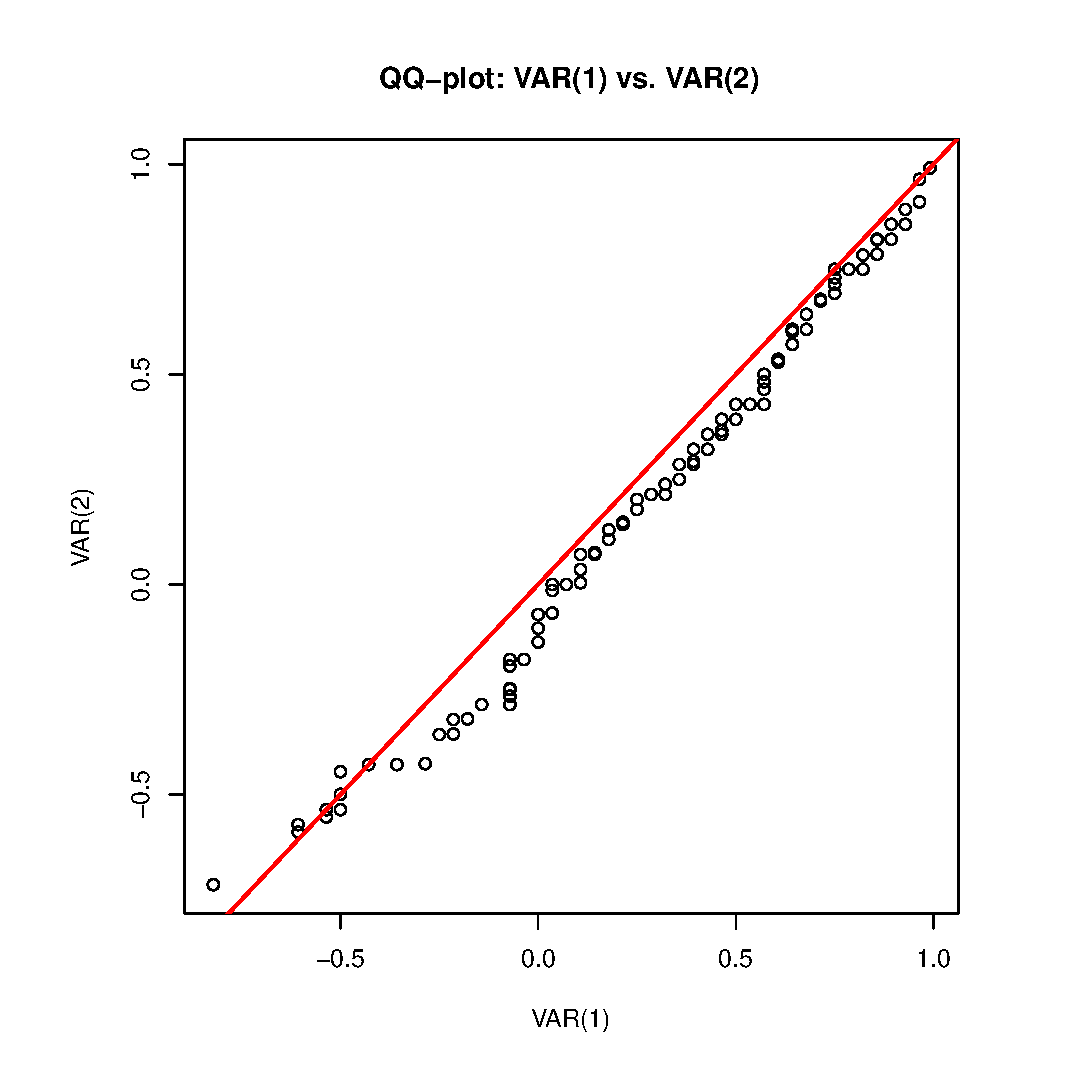
\includegraphics[scale=0.275]{Figure_7c.eps}
\end{tabular}
\caption{Histogram of Spearman correlations between the observations and VAR(1) and VAR(2) model fits (left and right penal, respectively). The third panel contains the QQ-plot of these two types of correlation.} \label{fig:compVAR1-2}  
\end{figure}


\begin{figure}[h!]
\centering
\begin{tabular}{c}
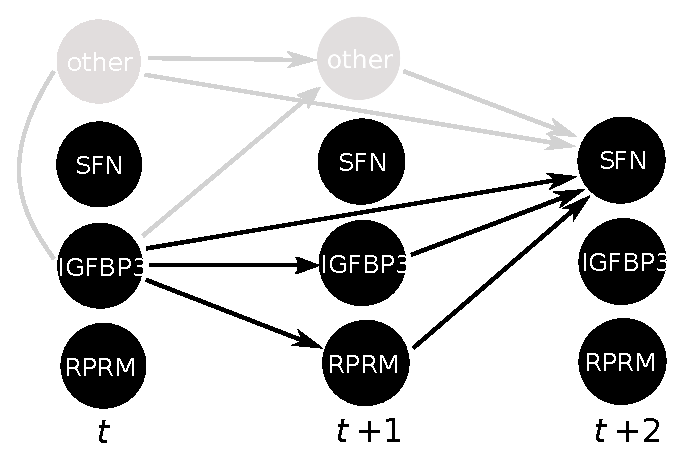
\includegraphics[scale=0.58]{VAR2pathsExample.eps}
\end{tabular}
\caption{Subgraph of the VAR(2) associated time-series chain graph, containing all paths connecting the IGFBP3 and SFN genes.}
\label{fig:VAR2pathDecomposition}  
\end{figure}


The covariance of the expression levels of a gene at the current time point and that of another gene at a future time point may be decomposed in terms of the paths connecting them in the time series chain graph, thus clarifying the propagation of signals through the network. In general, the covariance between the $j_1$- and $j_2$-th variates at time points $t$ and $t + \tau$, respectively, is:
%\begin{eqnarray*}
\begin{flalign*}
\mbox{Cov}(\mathbf{Y}_{j_1, t, i}, \mathbf{Y}_{j_2, t+\tau, i} \, | \, \mathbf{Y}_{\ast, t -1, i}, \mathbf{Y}_{\ast, t -2, i}) & = & \sum_{j'=1}^p (\mathbf{\Sigma}_{\varepsilon})_{j_1, j'} \sum_{ \substack{ \ell_0=0, \ell_m \in \{ 0, 1, 2\} \\ \sum \ell_m = \tau} } \Big( \prod_{m=0}^{\tau} \mathbf{A}_{\ell_m}^{\top} \Big)_{j', j_2}, \qquad
\end{flalign*}
%\end{eqnarray*}
where $\mathbf{A}_{0} = \mathbf{I}_{pp}$. The covariance can be further decomposed by expansion of the product of the (sparse) autoregression parameters $\mathbf{A}_1$ and $\mathbf{A}_2$ to obtain the contributions of all temporal paths connecting $j'$ and $j_2$ and, similarly, using the work of \cite{Jones2005} of the contemporaneous $(j_1, j')$-paths contributions. This is illustrated on the covariance between the IGFBP3 and SFN genes' expression levels two time points apart, equalling $-0.0142$. Figure \ref{fig:VAR2pathDecomposition} depicts the paths connecting these genes with the three paths contributing most to the covariance singled out. That is, the covariance is dominated by the temporal paths $Y_{\mbox{{\tiny IGFBP3}},t} \rightarrow Y_{\mbox{{\tiny SFN}},t+2}$, $Y_{\mbox{{\tiny IGFBP3}},t} \rightarrow Y_{\mbox{{\tiny IGFBP3}},t+1} \rightarrow Y_{\mbox{{\tiny SFN}},t+2}$, and $Y_{\mbox{{\tiny IGFBP3}},t} \rightarrow Y_{\mbox{{\tiny RPRM}},t+1} \rightarrow Y_{\mbox{{\tiny SFN}},t+2}$. Their contributions amount to $0.646$, $-0.0304$ and $-0.0211$, respectively, which accounts for 66.7\% (=38.3\% + 16.8\% + 11.6\%, respectively) of the absolute decomposed covariance contributions. The remaining 33.3\% is distributed over fourteen alternative paths involving seven other genes. Clearly, the IGFBP3 gene affects the SFN gene directly, but there is some attenuation via other routes of the network.



\section{Multiple VAR(1) models}
The sample information of the time-course experiment previously modelled by the VAR(1) model is now overlayed by group information (e.g. transfected by HPV16 or HPV18). One may then wish to highlight differences between the groups' time-series chain graphs. We focus on differential temporal relations between these graph. To this end we propose to estimate the autoregression coefficient matrices of the groups jointly employing the fused ridge estimator.

Still $n$ samples (cell lines) are followed over time and multivariately interrogated at regular intervals. Previously, the samples formed a single group i.i.d. distributed. Now the samples are divided in $G$ groups (e.g. induced by different treatments administered). The samples are indexed by $i=1, 2, \ldots, n_1, n_1 + 1 , \ldots, n_2, n+2 +1, \ldots 1+\sum_{g'=0}^{G-1} n_{g'}, \ldots, \sum_{g'=0}^{G} n_{g'}$ with $n_0 = 0$, $n_g$ the number of samples of the $g$-th group for $g=1, \ldots, G$, and $n=n_1+ n_2 + \ldots + n_g$. Within each group are modeled by a VAR(1) model:
%\begin{eqnarray*}
\begin{flalign*}
\left\{
\begin{array}{rclll}
\mathbf{Y}_{\ast, t, i} &  = & \bnu_1 + \mathbf{A}_1 \mathbf{Y}_{\ast, t-1, i} + \bvarepsilon_{\ast, t, i} & \mbox{for } i=1, \ldots, n_1 & \mbox{ and } t=1, \ldots, \mathcal{T},
\\
\mathbf{Y}_{\ast, t, i} &  = & \bnu_2 + \mathbf{A}_2 \mathbf{Y}_{\ast, t-1, i} + \bvarepsilon_{\ast, t, i} & \mbox{for } i=n_1+1, \ldots, n_2 & \mbox{ and } t=1, \ldots, \mathcal{T},
\\
\ldots &  = & \ldots & \ldots
\\
\mathbf{Y}_{\ast, t, i} &  = & \bnu_G + \mathbf{A}_G \mathbf{Y}_{\ast, t-1, i} + \bvarepsilon_{\ast, t, i} & \mbox{for } i=n_{G-1}+1, \ldots, n_G & \mbox{ and } t=1, \ldots, \mathcal{T}.
\end{array}
\right.
\end{flalign*}
%\end{eqnarray*}
where $\mathbf{Y}_{*,t,i}$ and $\bvarepsilon_{\ast,  t, i}$ $p$-dimensional random vectors representing respectively the variates and innovations. The latter with the usual normality assumption accompanying the VAR(1) model. Per group this gives three parameters $\bnu_g$, $\mathbf{A}_g$ and $\mathbf{\Sigma}_{\varepsilon, g}$. As before we assume $\bnu_g = \mathbf{0}_p$ for all $g$ (an assumption satisfied through (variate$\times$sample)-wise centering of the data). In principle, the remaining parameters could be estimated in group-wise fashion using the machinery developed by 
\cite{Miok2017}. However, groups need not differ (substantially) and much of the structure of VAR-processes is shared among the groups. For instance, different human papilloma viruses inserted in the same cell line may affect the gene-gene interactions of a pathway differently, but are unlikely to redesign the interaction patterns completely. Would such a scenario be plausible, it is then inefficient to estimate the parameters per group separately. The estimation may benefit when information among samples is borrowed. This is done in two ways. First, we assume the innovations stem from the same distribution through $\mathbf{\Sigma}_{\varepsilon, g} = \mathbf{\Sigma}_{\varepsilon}$ for all $g$.  This need not be realistic, but primary interest is in the temporal relations among variates captured by the auto-regression parameters $\mathbf{A}_1, \ldots, \mathbf{A}_G$. Practically (and of secondary importance), this assumption avoids the inclusion of (an) additional penalty parameter(s). More importantly, further information among the groups is borrowed in the estimation of the  $\mathbf{A}_g$'s. This will be done through the use of a so-called fused ridge penalty, which shrinks $\mathbf{A}_g$'s towards each other should the data give rise to it and refrains from doing so if the data contains no indication in this direction.


The model parameters $\mathbf{A}_1, \ldots, \mathbf{A}_G$ and $\mathbf{\Sigma}_{\varepsilon}$ are estimated by means of fused ridge penalized maximum likelihood. This exploits the $1^{\mbox{{\tiny st}}}$ order Markov property which, together with the distributional assumptions above, gives \\ $\mathbf{Y}_{\ast,t,i}|\mathbf{Y}_{\ast,t-1,i} \sim \mathcal{N}\left(\mathbf{A}_g \mathbf{Y}_{\ast, t-1,i},\boldsymbol{\Sigma}_{\varepsilon}\right)$ for $i \in \{1+ \sum_{g'=0}^{g-1} n_{g'}, \ldots, \sum_{g'=0}^{g} n_{g'} \}$. The joint log-likelihood function, defined as the group-wise sum of the marginal log-likelihoods, is:
\begin{eqnarray*}
\mathcal{L}(\mathbf{Y};\mathbf{A}_1, \ldots, \mathbf{A}_G, \mathbf{\Omega}_{\varepsilon}) & \propto & \sum_{g=1}^{G} \sum_{i=1+n_{g-1}}^{n_g} \sum_{t=2}^{\mathcal{T}} \big[
\log ( |\mathbf{\Omega}_{\varepsilon} |)
\\
& &   - \frac{1}{2} ( \mathbf{Y}_{\ast,t,i}  - \mathbf{A}_g \mathbf{Y}_{\ast,t-1,i} )^\top \mathbf{\Omega}_{\varepsilon} ( \mathbf{Y}_{\ast,t,i} - \mathbf{A}_g \mathbf{Y}_{\ast,t-1,i} ) \big].
\end{eqnarray*}
The log-likelihood function $\mathcal{L}$ is penalized by ridge penalties on the $\mathbf{A}_g$'s and $\mathbf{\Omega}_{\varepsilon}$:
\begin{eqnarray*}
\tfrac{1}{2} (\mathcal{T} - 1) \lambda_{\omega} \sum_{g=1}^G n_g  \| \mathbf{\Omega}_{\varepsilon} - \mathbf{\Omega}_0 \|_2^2 + \tfrac{1}{2} (\mathcal{T} - 1) \lambda_a \sum_{g=1}^G n_g  \| \mathbf{A}_g -  \mathbf{A}_0 \|_2^2
\end{eqnarray*}
in combination with fused ridge penalties on $\mathbf{A}_g$'s:
\begin{eqnarray*}
&  &  \tfrac{1}{2} (\mathcal{T} - 1) \lambda_f \sum_{g_1=1}^G n_{g_1}   \sum_{ \substack{ g_2=1 \\ g_2 \not= g_1} }^G  \| \mathbf{A}_{g_1} - \mathbf{A}_{g_2} \|_2^2,
\end{eqnarray*}
where $\mathbf{A}_0$ and $\mathbf{\Omega}_0$ are non-random  target matrices common to all groups, ridge penalty parameter $\lambda_a$ and $\lambda_{\omega}$, and the fusion penalty parameter $\lambda_f$ determining the degree to which the $\mathbf{A}_g$ are shrunken towards each other.

The maximization of this fused ridge penalized log-likelihood proceeds along the same lines as that of the ridge penalized log-likelihood of the VAR(1) model. First, the estimator of each $\mathbf{A}_g$, given the others and $\mathbf{\Omega}_{\varepsilon}$, is derived. This is followed by that of $\mathbf{\Omega}_{\varepsilon}$ given those of the $\mathbf{A}_g$'s. These are combined in an iterative procedure to produce the final estimates. 

The estimators of the $\mathbf{A}_g$ are found by equating the first order derivative (w.r.t $\mathbf{A}_g$) of the fused ridge penalized log-likelihood to zero and solving for $\mathbf{A}_g$, treating the other variables as non-random. Matrix algebra similar to that used in the derivation of the ridge penalized ML estimators of the VAR(1) model parameters gives:
\begin{eqnarray*}
\mbox{vec}[ \hat{\mathbf{A}}_g(\lambda,\lambda_f) ] & = & \{ n_g (\mathcal{T}-1) [ \lambda_a + (G-1)\lambda_f ] \mathbf{I}_{p^2\times p^2} + \widehat{\mathbf{\Gamma}}_g(0) \otimes \mathbf{\Omega}_{\varepsilon} \}^{-1}
\\
& & \{ n_g (\mathcal{T}-1) [\lambda_a \mbox{vec}(\mathbf{A}_0) + \lambda_f \sum_{ \substack{ g'=1 \\ g' \not= g} }^G \mbox{vec}(\mathbf{A}_{g'}) ] + \textrm{vec} [ \mathbf{\Omega}_{\varepsilon} \widehat{\mathbf{\Gamma}}_g(-1) ] \},
\end{eqnarray*}
where $\widehat{\mathbf{\Gamma}}_g(0) = \tfrac{1}{n_g(\mathcal{T}-1)} \sum_{i=1}^{n_g}\sum_{t=2}^{\mathcal{T}} \mathbf{Y}_{\ast,t-1,i}\mathbf{Y}_{\ast,t-1,i}^{\top}$ and \\
 $\widehat{\mathbf{\Gamma}}_g(-1) = \tfrac{1}{n_g(\mathcal{T}-1)} \sum_{i=1}^{n_g} \sum_{t=2}^{\mathcal{T}} \mathbf{Y}_{\ast, t, i} \mathbf{Y}_{\ast,t-1,i}^{\top}$, the estimates of the variance and lag $-1$ covariance of the $g$-th group. For the ridge ML estimator of the common precision matrix of the innovations $\boldsymbol{\Omega}_{\varepsilon}$, we need the sample covariance matrix of the innovations:
\begin{eqnarray*}
\mathbf{S}_{\varepsilon} =
\sum_{g=1}^{G} \frac{1}{n_g(\mathcal{T}-1)}
\sum_{i=1+n_{g-1}}^{n_g} \sum_{t=2}^{\mathcal{T}} \left[\mathbf{Y}_{\ast,t,i} - \mathbf{A}_g \mathbf{Y}_{\ast,t-1,i} \right] \left[\mathbf{Y}_{\ast,t,i} - \mathbf{A}_g\mathbf{Y}_{\ast,t-1,i} \right]^{\top}.
\end{eqnarray*}
The ridge estimate of $\boldsymbol{\Omega}_{\varepsilon}$ is then (with the same properties) as in the VAR(1) case only with this sample covariance matrix replacing that of the non-fused case.

The estimators above are combined in an iterative procedure to obtain the joint ML estimators of the $\mathbf{A}_g$'s and $\boldsymbol{\Omega}_{\varepsilon}$. The procedure is initiated with the marginal ridge LS estimates of the $\mathbf{A}_g$'s. These are obtained through the group-wise fit of  the VAR(1) model with $\boldsymbol{\Omega}_{\varepsilon} = \mathbf{I}_{pp}$. The first step of the iterative estimation procedure then comprises the estimation of $\boldsymbol{\Omega}_{\varepsilon}$ (given the initial estimates of $\mathbf{A}_g$). This is followed by the estimation of the $\mathbf{A}_g$'s. Running over the groups, each $\mathbf{A}_g$ is estimated keeping the other $\mathbf{A}_g$'s and $\boldsymbol{\Omega}_{\varepsilon}$ fixed. This is done until sequential estimates of each $\mathbf{A}_g$ differ less than a user-specified threshold. Once this is achieved, the procedure returns to the estimation of $\boldsymbol{\Omega}_{\varepsilon}$. And so on, until convergence.


The methodology for joint learning of multiple VAR(1) models through the fused ridge approach is illustrated on mRNA gene expression data from the aforementioned experiment with HPV16 and HPV18 group information overlayed. The optimal penalty parameters selected through maximization of the LOOCV log-likelihood are $\lambda_a=19.4444$, $\lambda_f=21.9996$ and $\lambda_{\omega}=0.0024$. Their optimality has been be checked visually by contour plots of the LOOCV log-likelihood versus penalty parameters (Figure 4.3, \cite{Supp2018}). Using the optimal penalty parameters non-sparse model parameters $\mathbf{A}_g$ and $\boldsymbol{\Omega}_{\varepsilon}$ are estimated.


The support of the model parameters is determined from the fused ridge parameter estimates. Sparsification of the $\mathbf{A}_g$'s and $\boldsymbol{\Omega}_{\varepsilon}$ proceeds as for VAR(1) model (cf. \cite{Miok2017}) with the support being determined for each of the $g$ autoregressive model parameter separately. The inferred number of nonzero autoregression parameters is 88 and 125 for the HPV16 and HVP18 affected cell lines, respectively. The excess of inferred interactions of the HPV18 cell line model may be due to the HPV16 being more oncogenic than the HPV18. The HPV16 may achieve this through more aggressive disruption of the cellular regulatory network, leading to less preserved interactions. Fewer interactions indicate less cohesion, in turn corresponding to less control of the network and increasing the potential for oncogenesis \citep{Wieringen2015}. This observation might be linked to the varying degree in p53 degradation observed for different oncogenic HPV types \citep{Schutze2014}. Inferred (non)-zero elements of the $\mathbf{A}_g$'s and $\boldsymbol{\Omega}_{\varepsilon}$ are then used to re-estimate these parameters, but per group the VAR(1) model is now fitted separately due to their support being different. The group-wise optimal penalty parameters are $\lambda_{a}=1.4077$, $\lambda_{\omega}=0.0045$ for cell lines affected with HPV16 and $\lambda_{a}=1.0967$, $\lambda_{\omega}= 0.0053$ for those affected with HPV18. The optimality of the penalty parameters are verified using contour plots. The penalty parameters $\mathbf{A}$ and $\mathbf{\Omega}_{\varepsilon}$ are comparable in size between the groups. The resulting group-wise re-estimated -- incorporating the inferred support -- model parameters are thus also comparable. The overlap and contrast of the HPV16 and HPV18 time-series chain graph derived from the re-estimated VAR(1) parameters for both groups are displayed in Figure \ref{fig:VARmultipleEst}. This reveals a substantial amount of overlap but even more differences, with plenty of virus specific edges. 

\begin{figure}[h!]
\centering
\begin{tabular}{cccc}
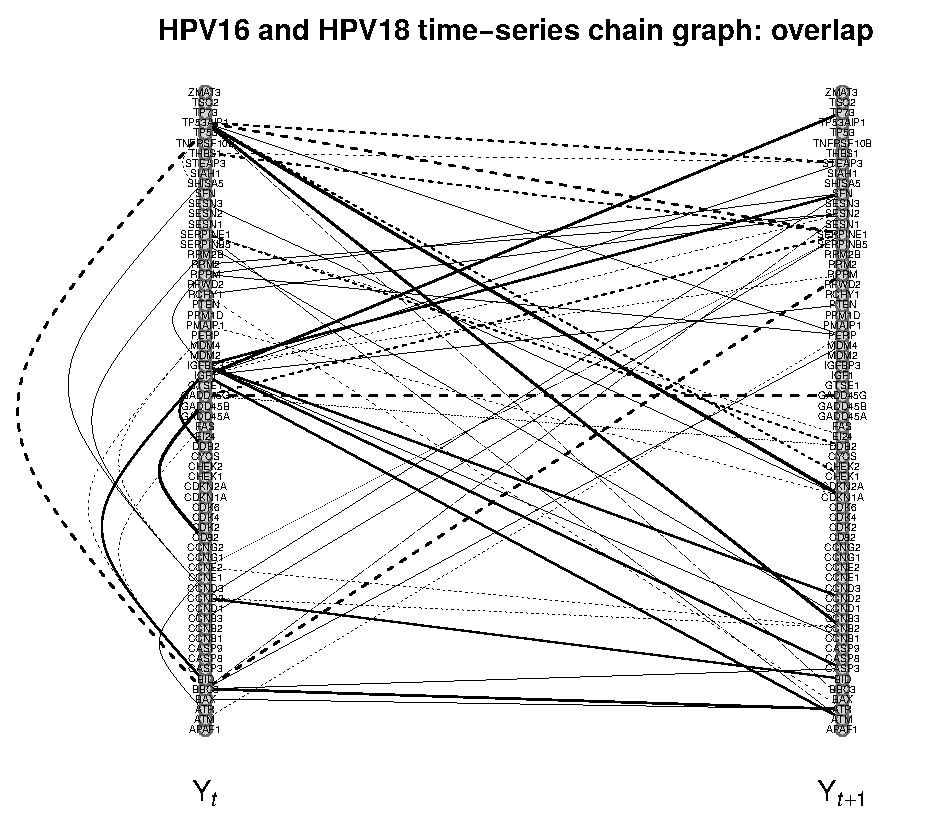
\includegraphics[scale=0.47]{Figure_11c.eps} & & &
\includegraphics[scale=0.45]{Figure_11d.eps}
\end{tabular}
\caption{Left and right panels depict the overlap and contrast, respectively, of the inferred time-series chain graphs from the cell lines affected with HPV16 and HPV18. Solid and dashed lines represent positive and negative relations, respectively. Black lines are common to the time-series chain graphs of both viruses, while the  blue and red lines are present in the graphs of the HPV16 and HPV18 (respectively) only. The thickness of the lines corresponds to the strength of the relation.}
\label{fig:VARmultipleEst}
\end{figure}


Post-estimation analysis of the VAR(1) model may shed light on the differential gene expression dynamics implied by different VAR(1) models. This is done by the downstream analyses introduced for the VAR(1) model. For instance, group-wise impulse response analysis may reveal how  a unit change in gene expression levels at the current time point $t$ differentially affects the gene expression level at time point $t+\tau$. Similarly, the differentially association between a variate at the current time and those at a future time may be identified from the group-wise mutual informations. Finally, comparison of group-wise path decompositions may point to the cross-group re-wiring of the connectivity of two nodes. Downstream analysis using re-estimated model parameters may also comprise of the calculation of network summary measures \citep{Newman2010}. For the five top `regulators' and `regulatees' node statistics are calculated and shown in Table \ref{table:postEstNodeStats} for the HPV16 and HPV18  cell lines. Comparison of both table reveals that there is a large overlap in `regulators' and `regulatees'. In both gene-type categories there is a notable difference. IGF1 and CCNB3 are a top `regulator' and `regulatee', respectively, in the VAR(1) description of the P53 signalling pathway from the HPV16. These are replaced by CCND2 and PERP, respectively, in the HPV18 data based pathway model. These differences shed light on the differential oncogenic potential of the two HPV varieties as was also shown by differences in immortalising capacity related to copy number alterations {\cite{Schutze2014, Schutze2016}.


\begin{table}
\caption{Node statistics for the top five `regulators' and `regulatees' (as derived from the time-series chain graph of the p53 signaling pathway) identified from the HPV16 and HPV18 affected cell line data using the estimated VAR(1) models. The left most column indicates the HPV variant, followed by the names of these genes. The next columns give the following node statistics: the in- and out-degree of the lag-one temporal dependencies; betweenness in the (global) partial correlation graph, closeness in the (global) partial correlation graph, the mutual information between the expression level of the gene at time $t$ and all other genes from the pathway at time $t+1$, and the impulse response in the gene at time $t$ on all other genes at time $t+1$.}
\begin{tabular}{ll*{6}{c}r}
\hline
\hline          
HPV & gene & $\mbox{deg}^-(\mathbf{A})$ & $\mbox{deg}^+(\mathbf{A})$ & betw. & close. & mut. info. & imp. resp.  \\
\hline
16 & BBC3        & 0 & 12 & 27 & 0.00029 & 0.08711 & 0.01584
\\
16 & IGF1     & 0 & 11 & 0 & 0.00025 & 0.03266 & 0.01112
\\
16 & IGFBP3     & 0 & 10 & 17 & 0.00029 & 0.09925 & 0.01798
\\
16 & TP53AIP1     & 1 & 9 & 1 & 0.00025 & 0.11136 & 0.01536
\\
16 & THBS1     & 0 & 6 & 0 & 0.00024 & 0.03132 & 0.00882
\\
\\
16 & CCNB3    & 10 & 1 & 0 & 0.00024 & 0.00065 & 0.00042
\\
16 & SESN2        & 7 & 1 & 0 & 0.00024 & 0.02017 & 0.00176
\\
16 & SERPINE1       & 6 & 5 & 0 & 0.00024 & 0.04194 & 0.00683
\\
16 & STEAP3    & 5 & 0 & 0 & 0.00024 & 0.00000 & 0.00000
\\
16 & CDKN2A  & 5 & 0 & 0 & 0.00024 & 0.00000 & 0.00000
\\
\\
\\
18 & IGFBP3        & 0 & 17 & 17 & 0.0029 & 0.16543 & 0.02502
\\
18 & CCND2     & 1 & 15 & 24 & 0.0029 & 0.02642 & 0.01705
\\
18 & BBC3     & 0 & 15 & 27 & 0.0029 & 0.09903 & 0.02233
\\
18 & TP53AIP1     & 0 & 10 & 1 & 0.0028 & 0.05642 & 0.01784
\\
18 & THBS1     & 1 & 11 & 0 & 0.0028 & 0.09053 & 0.01906
\\
\\
18 & PERP    & 12 & 0 & 0 & 0.0027 & 0.00000 & 0.00000
\\
18 & SERPINE1        & 7 & 3 & 0 & 0.0027 & 0.02247 & 0.00465
\\
18 & CDKN1A       & 6 & 0 & 0 & 0.0025 & 0.00000 & 0.00000
\\
18 & STEAP3 & 5 & 0 & 0 & 0.0025 & 0.00000 & 0.00000
\\
18 & SESN2  & 5 & 1 & 0 & 0.0026 & 0.00016 & 0.00023
\\
\hline
\hline
\end{tabular}
\label{table:postEstNodeStats}
\end{table}


Finally, the path decomposition analysis of the covariance -- outlined for the VAR(1) model -- is applied to the HPV16 and HPV18 VAR(1) models seperately to identify differential regulatory patterns. This is done for the (IGFBP3, SESN2) gene pair and we thus decompose $\mbox{Cov}(Y_{IGFBP3,t}, Y_{SESN2,t+1}) = (\mathbf{\Sigma}_{\varepsilon} \mathbf{A}^{\top})_{IGFBP3,SESN2}$. Although this reveals quantitative differences between the two decompositions, the details are omitted. More strikingly, the direct path between $Y_{IGFBP3,t}\rightarrow Y_{SESN2,t+1}$ has vanished in the HPV18 description of the P53 pathway. This hints at differential regulation.

\section{The VARX(1) model} 
When having measured multiple molecular levels, an integrative view of the levels' networks  comes within reach. In addition to the `within-level' relations among variates, this also encompasses relations between different molecular levels (e.g. how does a DNA copy number change affect a gene's mRNA expression levels). Here this is done by extending the VAR(1) model to a VARX(1) model which allows the inclusion of time-varying covariates (responsible for the X in VARX) like DNA copy number or microRNA expression. Within the VARX(1) model the molecular levels are no longer on a par. It differentiates between an endogeneous (e.g. mRNA expression) and an exogeneous level (e.g. DNA copy number). In addition to the `between-level' relations that may now be reconstructed, the inclusion of the exogeneous level aids in the reconstruction of the underlying network of the endogeneous one. 

Consider a time-course microarray experiment comprising $n$ cell lines (samples) that followed during $\mathcal{T}$ consecutive time points. At each time point, all samples' variates stemming from multiple molecular levels (at least two e.g. DNA copy number, mRNA or miRNA gene expression) are measured. The endogeneous variates (e.g. the mRNA gene expression levels) of sample $i$ at time point $t$ are represented by the $p$-dimensional random vector $\mathbf{Y}_{*,t,i}$. Similarly, the $q$-dimensional variable $\mathbf{X}_{*,t,i}$ denotes the exogeneous variates (e.g. DNA copy number or miRNA gene expression levels) of sample $i$ at time point $t$.


Let the data from this experiment be modeled by a first-order vector autoregressive with a time-varying covariate, abbreviated to VARX(1), model:
\begin{eqnarray*}
\mathbf{Y}_{*,t,i} & = & \boldsymbol{\nu}+\mathbf{A} \mathbf{Y}_{*,t-1,i} + \mathbf{B} \mathbf{X}_{*,t,i} + \boldsymbol{\varepsilon}_{*,t,i},
\end{eqnarray*}
with intercept vector $\nu=\mathbf{0}_{p}$, $q$-dimensional exogenous time-varying covariate vector $\mathbf{X}_{*,t,i}$ of sample $i$ at time $t$, the $p \times p$-dimensional matrix $\mathbf{A}$ with auto-regression coefficients, the $p \times q$-dimensional matrix $\mathbf{B}$ with regression coefficients of the time-varying covariates, and $\boldsymbol{\varepsilon}_{*,t,i}$ an error vector of length $p$. The errors are assumed to be identically and independently distributed as $\boldsymbol{\varepsilon}_{*,t,i} \sim \mathcal{N}( \mathbf{0}, \mathbf{\Sigma}_{\varepsilon})$.

Due to the independence among the samples and the Markov property of the VARX(1) model, the likelihood is:
\begin{eqnarray*}
\hspace{-1.0cm} L(\mathbf{Y};\mathbf{X},\mathbf{A},\mathbf{B},\boldsymbol{\Sigma}_{\varepsilon}) & = & \prod_{i=1}^n \prod_{t=2}^{\mathcal{T}}P(\mathbf{Y}_{*,t,i}|\mathbf{Y}_{*,t-1,i},\mathbf{X}_{*,t,i}).
\end{eqnarray*}
Use $\mathbf{Y}_{*,t,i} \, | \, \mathbf{Y}_{*,t-1,i},\mathbf{X}_{*,t,i}\sim \mathcal{N}\left(\mathbf{A} \mathbf{Y}_{*,t-1,i} + \mathbf{B} \mathbf{X}_{*,t,i},\boldsymbol{\Sigma}_{\varepsilon}\right)$ and take the logarithm to obtain the log-likelihood:
%\begin{eqnarray*}
\begin{flalign*}
\mathcal{L}(\mathbf{Y};\mathbf{X}, \mathbf{C}, \boldsymbol{\Sigma}_{\varepsilon}) & \propto &  - n(\mathcal{T}-1)\ln\left|\boldsymbol{\Sigma}_{\varepsilon}^{-1}\right|  -\frac{1}{2}\sum_{i=1}^n \sum_{t=2}^{\mathcal{T}}\left\{-\frac{1}{2}\left[\mathbf{Y}_{*,t,i}-  ( \mathbf{Z}_{*,t,i}^\top \otimes \mathbf{I}_{p\times p} ) \textrm{vec}(\mathbf{C}) \right]^\top\right. \qquad \qquad \qquad \qquad \qquad 
\\
& & \left.\boldsymbol{\Sigma}_{\varepsilon}^{-1}
\left[\mathbf{Y}_{*,t,i}-  (\mathbf{Z}_{*,t,i}^\top \otimes \mathbf{I}_{pp} ) \textrm{vec}(\mathbf{C}) \right] \right\}, \qquad \qquad \qquad \qquad  \qquad \qquad
%\end{eqnarray*}
\end{flalign*}
in which $\mathbf{C} = (\mathbf{A}|\mathbf{B})$ and thus $\textrm{vec}(\mathbf{C}) = \textrm{vec}(\mathbf{A}|\mathbf{B}) = [\textrm{vec}(\mathbf{A})^{\top},  \textrm{vec}(\mathbf{B})^\top ]^{\top}$, where the vec-operator stacks the columns of matrix into a vector. Moreover, $\mathbf{Z}_{*,t,i} = (\mathbf{Y}_{*,t-1,i}^{\top},  \mathbf{X}_{*,t,i}^{\top})^{\top}$.

To accommodate the high-dimensionality of the data the log-likelihood
is augmented with ridge penalties on $\mathbf{A}$, $\mathbf{B}$ and $\mathbf{\Sigma_{\varepsilon}}$:
\begin{eqnarray*}
& & \hspace{-2cm} \mathcal{L}^{\mbox{{\tiny pen}}}(\mathbf{Y};\mathbf{X},\mathbf{C},\boldsymbol{\Omega}_{\varepsilon};\lambda_a,\lambda_b,\lambda_{\omega},\mathbf{C}_0, \boldsymbol{\Omega}_0)
\\
& \propto & \mathcal{L}(\mathbf{Y};\mathbf{X},\mathbf{C}, \boldsymbol{\Omega}_{\varepsilon}) -\frac{n(\mathcal{T}-1)}{2}\lambda_{\omega}\textrm{tr}\left[(\boldsymbol{\Omega}_{\varepsilon}-\boldsymbol{\Omega}_{0})^\top(\boldsymbol{\Omega}_{\varepsilon}-\boldsymbol{\Omega}_{0})\right]
\\
& & -\frac{n(\mathcal{T}-1)}{2}\textrm{tr}\left\{\left[\textrm{vec}( \mathbf{C})-\textrm{vec}(\mathbf{C}_0) \right]^\top \mathbf{\Lambda}_c \left[\textrm{vec} (\mathbf{C})-\textrm{vec}(\mathbf{C}_0) \right]\right\}
\end{eqnarray*}
in which $\boldsymbol{\Omega}_{\varepsilon} = \boldsymbol{\Sigma}_{\varepsilon}^{-1}$, user-specified, non-random target matrices $\mathbf{A}_0$, $\mathbf{B}_0$ and $\mathbf{\Omega}_0$, $\mathbf{C}_0 = (\mathbf{A}_0 | \mathbf{B}_0)$, and the $p(p+q) \times p(p+q)$ dimensional, diagonal matrix $\mathbf{\Lambda}_c$ with $(\mathbf{\Lambda}_c)_{jj} = \lambda_a$ for $j = 1, \ldots, p^2$ and $(\mathbf{\Lambda}_c)_{jj} = \lambda_b$ for $j = p^2 + 1, \ldots, p^2 + pq$. Note that this penalty term involving $\mathbf{C}$ is proportional to the algebraic ridge penalties $\| \mathbf{A} \|^2_2 + \| \mathbf{B} \|^2_2$.

An estimator for  $\mathbf{C}$ is now found by solving its estimating equation (arrived at through equating the derivative of the penalized log-likelihood with respect to $\mathbf{C}$ to zero). Grouping of terms and solving for $\mathbf{C}$ yields the ridge ML estimator:
\begin{eqnarray*}
\textrm{vec} [\widehat{\mathbf{C}}(\boldsymbol{\Lambda}_c) ] & = & [\boldsymbol{\Lambda}_c+\tilde{\boldsymbol{\Gamma}}_{zz}(0) \otimes \boldsymbol{\Omega}_{\varepsilon} ]^{-1} \{\boldsymbol{\Lambda}_c\textrm{vec}(\mathbf{C}_0) + \textrm{vec}  [\boldsymbol{\Omega}_{\varepsilon} \otimes \tilde{\boldsymbol{\Gamma}}_{yz}(-1) ] \},
\end{eqnarray*}
where
%\begin{eqnarray*}
\begin{flalign*}
\tilde{{\boldsymbol{\Gamma}}}_{zz}(0)=\frac{1}{n(\mathcal{T}-1)}\sum_{i=1}^{n}\sum_{t=2}^{\mathcal{T}} \mathbf{Z}_{*,t,i}\mathbf{Z}_{*,t,i}^{\top} \quad \mbox{ and  } \quad \tilde{\boldsymbol{\Gamma}}_{yz}(-1) = \frac{1}{n(\mathcal{T}-1)} \sum_{i=1}^{n} \sum_{t=2}^{\mathcal{T}}\mathbf{Y}_{*,t,i} \mathbf{Z}_{*,t,i}^{\top}.
\end{flalign*}
%\end{eqnarray*}
The ridge estimator of $\mathbf{C}$ involves the Kronecker product which frustrates its numerical evaluation for even moderately sized $p$ and $q$ (as it involves matrices of dimensions $(p^2 + pq) \times (p^2 + pq)$. Previously with the VAR(1) model, this was circumvented by rewriting the estimator. The same can be done here, but requires an approximation of the inverse in the ridge estimator of $\mathbf{C}$. For the approximation, write $\nu_1 = {\textstyle\frac{1}{2}} (\lambda_a + \lambda_{b})$ and $\nu_2 = {\textstyle\frac{1}{2}} (\lambda_a - \lambda_{b})$. Then:
\begin{flalign*}
%\begin{eqnarray*}
[\boldsymbol{\Lambda}_c + \tilde{\boldsymbol{\Gamma}}_{ZZ}(0) \otimes \boldsymbol{\Omega}_{\varepsilon}]^{-1} & = & \left[ \nu_1 \mathbf{I}_{p(p+q) \times p(p+q)} + \nu_2
\left(
\begin{array}{rr}
\mathbf{I}_{p^2 \times p^2} & \mathbf{0}_{p^2 \times pq}
\\
\mathbf{0}_{pq \times p^2} & - \mathbf{I}_{pq \times pq}
\end{array}
\right)
+ \tilde{\boldsymbol{\Gamma}}_{ZZ}(0) \otimes \boldsymbol{\Omega}_{\varepsilon} \right]^{-1} 
\\
& \approx & \mathbf{\Theta}^{-1} - \nu_2 \mathbf{\Theta}^{-1} \left(
\begin{array}{cc} \mathbf{I}_{p^2 \times p^2} & \mathbf{0}_{p^2 \times pq}
\\
\mathbf{0}_{pq \times p^2} & - \mathbf{I}_{pq \times pq}
\end{array}
\right) \mathbf{\Theta}^{-1} \qquad \qquad \qquad \qquad \quad
\\
& = & \mathbf{\Theta}^{-1} - \nu_2 \mathbf{\Theta}^{-2}  + 2 \nu_2 \mathbf{\Theta}^{-1} \left(
\begin{array}{cc} \mathbf{0}_{p^2 \times p^2} & \mathbf{0}_{p^2 \times pq}
\\
\mathbf{0}_{pq \times p^2} & - \mathbf{I}_{pq \times pq}
\end{array} \right) \mathbf{\Theta}^{-1}, \qquad \qquad
%\end{eqnarray*}
\end{flalign*}

where $\mathbf{\Theta} =  \nu_1 \mathbf{I}_{p(p+q) \times p(p+q)}
+ \widetilde{\boldsymbol{\Gamma}}_{ZZ}(0)\otimes\boldsymbol{\Omega}_{\varepsilon}$.
The eigen-decomposition can readily be applied to the first two terms in the approximation. But also to the last as only a subset of the eigenvectors share the same nonzero eigenvalue.

Again the ridge ML estimator of the error precision, $\boldsymbol{\Omega}_{\varepsilon}$, is given in display (\ref{ridgePrecision}) with the sample error covariance now:
%\begin{eqnarray*}
\begin{flalign*}
\mathbf{S}_{\varepsilon} = \frac{1}{n(\mathcal{T}-1)}\sum_{i=1}^{n}\sum_{t=2}^{\mathcal{T}}\left[\mathbf{Y}_{*,i,t}- \mathbf{A}\mathbf{Y}_{*,t-1,i} - \mathbf{B} \mathbf{X}_{*,t,i} \right] \left[\mathbf{Y}_{*,t,i} - \mathbf{A} \mathbf{Y}_{*,t-1,i} - \mathbf{B} \mathbf{X}_{*,t,i}\right]^{\top},
\end{flalign*}
%\end{eqnarray*}
substituted. 

The ridge penalized maximum likelihood estimates of $\mathbf{A}$, $\mathbf{B}$ and $\boldsymbol{\Omega}_{\varepsilon}$ may now be obtained by iteratively estimating one while keeping the other fixed. This iterative procedure is initiated by the ridge LS (least squares) estimate of $\mathbf{C}$, which is obtained from its ML counterpart by setting $\boldsymbol{\Omega}_{\varepsilon} = \mathbf{I}_{pp}$. As before penalty parameters $\lambda_a$, $\lambda_b$ and $\lambda_{\omega}$ are chosen to optimize the LOOCV log-likelihood.

Next we present the several downstream analyses in order to gain better understanding of the dynamics within and between the entities of the various molecular levels. 
\begin{compactitem}
\item  First the nonzero elements of model parameters $\mathbf{A}$, $\mathbf{B}$ and $\boldsymbol{\Omega}_{\varepsilon}$ are identified through sparsification (in a similar way as for the VAR(1) model). 

\item The impulse response analysis of the VARX(1) model assesses the effect of a change in an innovations or a time-varying covariate on a particular variate. This amounts to the evaluation of the derivative of the latter with respect to one of the former. Using the time-recursive definition of the VARX(1) model, this boils down to:
\begin{eqnarray*}
\frac{\partial \mathbf{Y}_{\ast,t+\tau,i}}{\partial \boldsymbol{\varepsilon}_{\ast,t,i}} & = & \mathbf{A}^{\tau} \qquad \mbox{ and } \qquad \frac{\partial \mathbf{Y}_{\ast,t+\tau,i}}{\partial \mathbf{X}_{\ast,t,i}} \, \, \,  = \, \, \,  \mathbf{A}^{\tau} \mathbf{B},
\end{eqnarray*}
with $\tau \in \mathbb{N}$. The $(j,k)$-th element of $\mathbf{A}^{\tau}\mathbf{B}$ represents the change in $Y_{j,t+\tau, i}$ due a unit change in $X_{k,t,i}$.

\item In the explanation of $\mathbf{Y}_{\ast, t, i}$ the VARX(1) model assumes the time-varying covariates to be non-random. When evaluating the mutual information terms involving any of the $\mathbf{X}_{j, t, i}$'s drop out. As a result conditional variances involved in the mutual information equal to that of the VAR(1) model, for which we refer to \cite{Miok2017}.
\end{compactitem}

The VARX(1) model related methodology is applied on the P53 signalling pathway data from the HPV-induced cell line experiment. In this interactions between the genes' DNA copy number and microRNAs on one hand and the mRNAs on the other are assumed to be known. With respect to the former only \textit{cis}-interactions are assumed to be physically feasible: a gene's dosage may only affect its own transcription directly (which in turn may then indirectly propagate through the network). The microRNA-mRNA interactions are taken from microRNA target prediction data bases. In particular, a microRNA-mRNA interaction requires for the mRNA to be the microRNA's target in at least two out of three data bases (targetscan, mirDB and RNA22). Optimal penalty parameters ($\lambda_a=255$, $\lambda_b=130$ and $\lambda_{\omega}=0.0034$) are verified using contour plots (Figure 4.3, \cite{Supp2018}) and used to arrive at estimates of the VARX(1) model parameters $\mathbf{A}$, $\mathbf{B}$ and $\mathbf{\Omega}_{\varepsilon}$. Support of the model parameters $\mathbf{A}$ and $\mathbf{\Omega}_{\varepsilon}$ is determined using the post-estimation selection procedure described earlier. 

The support of model parameters $\mathbf{A}$ and $\boldsymbol{\Omega}_{\varepsilon}$ (that of $\mathbf{B}$ is assumed known) is inferred through sparsification of their ridge estimates. The inferred support is used to re-estimate the model. Optimal penalty parameters are re-determined ($\lambda_a=0.6$, $\lambda_b=0.4868$ and $\lambda_{\omega}=0.0001$) and verified through contourplots (not shown). In Figure 4.4, \cite{Supp2018} the re-estimated model parameters are visualized as heatmaps, here only the time-series chain graph induced by these parameter is shown (Figure \ref{fig:graphVARX1})

\begin{figure}[h!]
\centering
\begin{tabular}{cc}
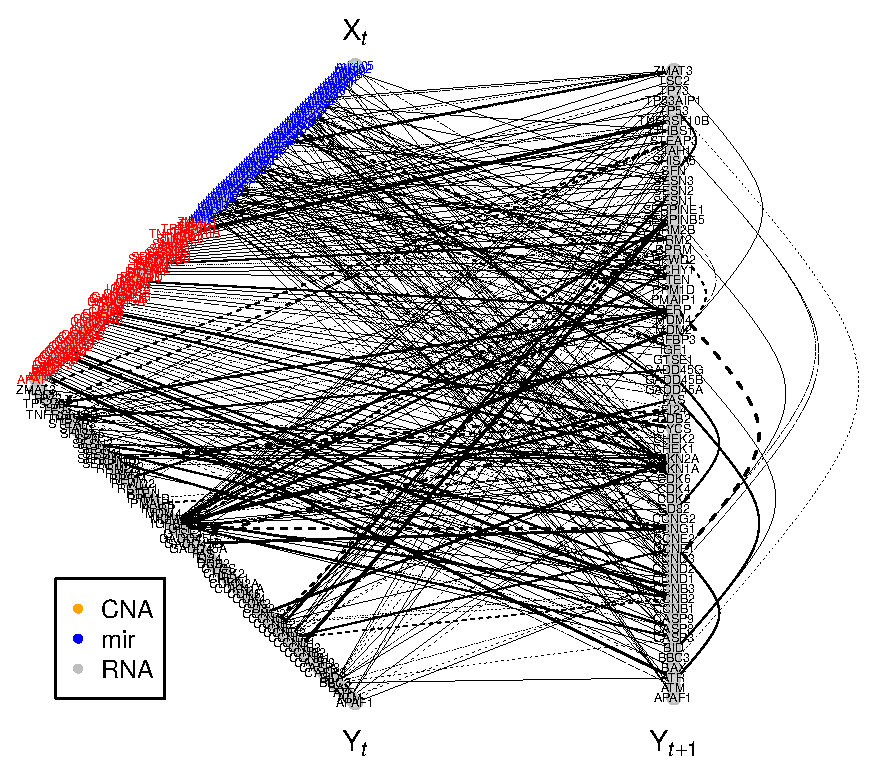
\includegraphics[scale=0.6]{Figure_17.eps}
\end{tabular}
\caption{Inferred time-series chain graph corresponding to the estimated VARX(1) model. Solid and dashed lines represent positive and negative relations, respectively. Line thickness corresponds to the strength of the relation. Unconnected nodes have been pruned from the graph.}
\label{fig:graphVARX1}
\end{figure}

The model parameters -- re-estimated obeying the inferred support -- are studied. We first turn our attention to the estimated matrix $\mathbf{B}$. The coefficients related to the DNA copy number effect are overwhemingly positive (as can be witnessed from the parameter heatmaps provided in Figure 4.4, \cite{Supp2018} or from the solid edges originating from the DNA copy number related nodes in Figure \ref{fig:graphVARX1}). This confirms the common-sense `larger gene dosage, more transcription' hypothesis. For miRNAs, (among others) breaking down mRNAs post-transcriptionnally, negative estimates of their effects are expected. Indeed, the largest (in an absolute sense) estimates are negative, but generally the miRNA related coefficients are a mixed bag containing both positive and negative estimates. As multiple miRNAs are known to target the same mRNA and proteins encoded by these mRNAs on the other hand could be involved in transcriptional regulation of the miRNAs, it is likely that many indirect effects are detected on the RNA level as well.


\begin{figure}[h!]
\centering
\begin{tabular}{c}
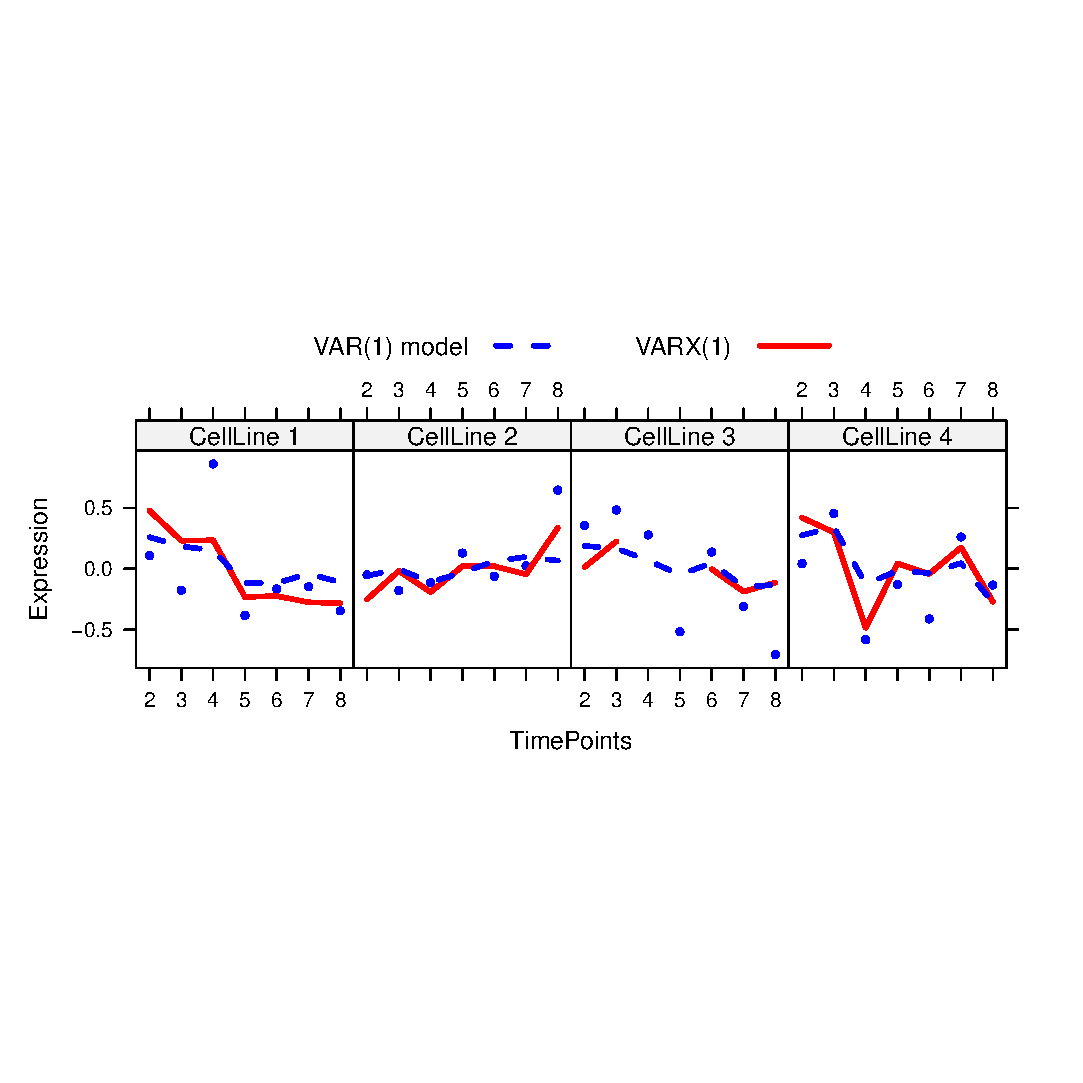
\includegraphics[scale=0.8]{Figure_14.eps}\\
\end{tabular}
\caption{Observations and VAR(1) and VARX(1) model fits of the CCNG1 expression data. Each panel, one per cell line, plots gene expression against time, excluding the first time point. The solid red and dashed green curves represents the fit of the VARX(1) and VAR(1) model fits, respectively. In the third cell line the VARX(1) model fit is interrupted due to failed microRNA hybridizations. 
}
\label{fig:CCNG1fitVAR1-VARX1}  
\end{figure}


The fitted VAR(1) and VARX(1) models exhibit various differences. Comparison of the temporal relations contained in the matrix $\mathbf{A}$ reveals only small changes in the endogenous part of the VAR(1) and VARX(1) models. For instance, both models share the same top `regulators', although these `regulators' affect more genes in VARX(1) model. Alternatively, both models may be compared by the study of their fit. Figure \ref{fig:CCNG1fitVAR1-VARX1} shows both fits for the gene CCNG1. More globally, the cell line-wise Spearman correlations between fitted and observed values of each gene may be compared between both models. Figure 4.8, \cite{Supp2018} contains the histograms of these correlations for VAR(1) and VARX(1) models. Notice that VARX(1) model has more correlations on right-hand side -- the positive part of the $x$-axis -- which implies an overall better fit. This improvement in fit is due a more complex model, using exogenous variables (DNA copy number and miRNA gene expression). To put this in perspective, the matrix $\mathbf{A}$ of the VAR(1) model contains 134 non-zero parameters, while the matrices $\mathbf{A}$ and $\mathbf{B}$ of VARX(1) model have 126 and 235 non-trivial parameters, respectively. 



\section{Conclusion}
The paper discussed the learning of molecular network models from high-dimensional multilevel molecular time-course data. This comprised their estimation, through penalized parameter estimation and support reconstruction,  as well as their exploitation to produce tangible consequences for the medical collaborator. Throughout the \texttt{ragt2ridges}-package, implementing the presented methodology, was used as a powerful means to this end. In the application of the developed methodology to a cervical study, serving as a running example, its potential for versatile analyses of the high-dimensional time-series omics data was demonstrated.

Further methodological and software development is envisioned in two directions. The most pressing is to facilitate analyses presented here using next generation sequencing data. As these data represent actual counts rather than intensities believed to be proportional to these counts, the Gaussian assumption of the presented models is untenable and need to be replaced by a more suitable alternative for sequencing data \citep{Heinen2003}. On the hand, all presented analyses assume linear relationships among the molecular entities. As a simple first order approximation this may be fine, but the true relationships may well be nonlinear \citep{Kantz2004}. It may be a lot to ask to learn more complex relationships from a limited number of time points and a strong guard against overfitting is necessary, but it would do more justice to the true dynamics of the cellular regulatory network.

\chapter{Comprehensive molecular profiling of HPV-induced transformation over time \\{\footnotesize(\textit{Miok, V., Babion, I., Jaspers, A., Meijer, C. J. L. M., Snijders, P. J. F., Steenbergen, R. D. M. , van Wieringen, W. N., Wilting, S. M., In preparation})}}
\chaptermark{Temporal profiling of HPV-induced transformation}
\label{chapter:Window estimator}

\graphicspath{{Chapter5/Figs/}{Chapter5/Figs/PDF/}{Chapter5/Figs/}}%


Although persistent infection with high-risk human papillomavirus (HPV) is generally acknowledged as necessary cause for cervical cancer, additional molecular changes are required for the progression from precancerous disease to cancer. Those changes include chromosomal aberrations and changes in DNA methylation patterns and result in deregulated expression of coding and non-coding RNAs. In this study we performed a comprehensive and longitudinal molecular characterization of HPV-transformed keratinocyte cell lines, to identify the sequential order and relevance of these molecular alterations for HPV-induced transformation.

Genome-wide chromosomal, mRNA - and miRNA expression profiles were generated from 4 HPV-transformed keratinocyte cell lines at 8 different passages representing distinct stages of transformation. Unsupervised hierarchical clustering in all 4 cell lines revealed that in particular copy number alterations are associated with the acquisition of anchorage independence, a hallmark of transformation. Approximately one third of differentially expressed mRNAs and miRNAs was directly attributable to DNA copy number alterations. Focal adhesion, TGF-$\beta$ signalling and mTOR signalling pathways were enriched among these genes. In addition, we identified potential miRNA-mRNA interactions over time, of which the BRWD3 and miR-221-3p interaction was confirmed \textit{in vitro}.

In conclusion, integrated longitudinal analysis of our HPV-induced transformation model enabled us to pinpoint relevant interconnected molecular changes and affected signalling pathways. Increased understanding of the interplay between different molecular alterations and thereby affected pathways  will be of importance for the identification of potential therapeutic targets as well as specific disease markers.
\\
\\
This chapter corresponds to the article:\\
 Miok, V., Babion, I., Jaspers, A., Meijer, C. J. L. M., Snijders, P. J. F. and Steenbergen, R. D. M. , van Wieringen, W. N., Wilting, S. M. Comprehensive molecular profiling of HPV-induced transformation over time. \textit{In preparation}.

\section{Introduction}

Development of cervical cancer is a multi-step process initiated by a persistent infection with a high-risk type of the human papillomavirus (HPV),  \cite{Walboomers1999}. Following infection of the basal epithelial cells by HPV, a productive infection is established, which is characterized by the production of new viral particles \cite{Chow2010, Steenbergen2014}. The expression of viral proteins is tightly linked to host cell differentiation and is necessary for viral genome replication in differentiated cells. Aberrant expression of viral oncogenes E6 and E7 in proliferating cells, however, leads to the abortion of the viral life cycle and triggers malignant transformation. While E6 and E7 initiate and maintain transforming infections, additional molecular changes in the host cell genome are required for the development of invasive cancer.

Molecular alterations associated with cervical carcinogenesis are of both genetic and epigenetic nature and ultimately lead to aberrant expression of oncoproteins and tumor suppressor proteins. Genome-wide analyses of cervical tissue specimens has led to the identification of numerous chromosomal aberrations and differentially expressed coding and non-coding genes in cervical (pre)cancer \cite{Thomas2014, Sopov2004, Wong2006, Srivastava2017, Hosseini2017}. As the sequential order of molecular changes as well as their causative relevance for cancer development cannot be extrapolated from cross-sectional data, it has proven problematic to distil promising disease markers and potential therapeutic targets from these observations. 

In vitro cell line models of HPV-mediated transformation in which primary keratinocytes are transfected with HPV16 or HPV18 have been shown to faithfully mimic cervical cancer development \cite{Steenbergen1996, Steenbergen2004, Wilting2006, Henken2007, Smeets2011}. This offers the unique opportunity to study (epi)genetic alterations over time. Integrative analysis of longitudinal data obtained from multiple molecular levels allows reconstruction of the sequential order in which molecular changes occur and is likely to result in the identification of crucial molecular alterations that drive the carcinogenic process. Previous studies have demonstrated that HPV-induced transformation can be divided into four stages (Figure \ref{fig:figure51} A) \cite{Chen1993, Steenbergen2005, Schutze2014}: an extended lifespan (1) is acquired as a result of E6 and E7 mediated inhibition of tumour suppressor genes p53 and pRb \cite{Moody2010, Klingelhutz2012}. Genetic instability induced by E6 and E7 subsequently generates an immortal phenotype (2) usually associated with the activation of the telomerase enzyme resulting from upregulation of hTERT. During prolonged culturing of HPV-immortalized keratinocytes additional (epi)genetic alterations accumulate that can eventually lead to anchorage-independent growth (3) and tumorigenicity (4). Anchorage independence in particular is considered evidence for complete transformation \textit{in vitro} \cite{Freedman1974, Mori2009}. Under normal circumstances detachment-induced cell death (anoikis) is induced by aberrant integrin signalling in epithelial cells that lost appropriate cell-cell and cell-matrix interactions. However, transformed epithelial cells can overcome this and subsequently grow anchorage- independently \cite{Guadamillas2011}. 

\begin{figure}[h!]
\centering
\begin{tabular}{cc} 
\includegraphics[scale=0.62]{Figure1.pdf}
\end{tabular}
\caption{Characterization of our longitudinal in vitro model system of hrHPV-induced transformation. In anchorage dependent (black) and independent (red) timepoints (T) of all 4 cell lines are shown in relation to the transformation process. MiRNA microarrays of cell line FK18A at T4 and T5 did not pass quality control and were therefore excluded from miRNA analysis. Unsupervised hierarchical cluster results based on \textbf{B} DNA copy number, \textbf{C} overall mRNA expression and \textbf{D} overall miRNA expression are shown for FK16A, FK16B, FK18A and FK18B.}
\label{fig:figure51}
\end{figure}

We here present the first comprehensive molecular profiling of HPV-induced transformation over time. DNA copy number changes, mRNA-, and miRNA expression were determined in 4 individual HPV-transformed keratinocyte cell lines at 8 different passages representing different stages of HPV-induced transformation (hereafter referred to as time points). Integrative temporal analysis of this unique longitudinal multi-level dataset allowed for the identification of relevant pathways and associated key regulators as well as the prediction of miRNA-mRNA interactions in HPV-induced transformation.

\section{Materials and methods}

\textbf{Cell lines and clinical specimens}
\\
Establishment and culture of the HPV16 (FK16A and FK16B) and HPV18 (FK18A and FK18B) immortalized keratinocyte cell lines has been described previously \cite{Steenbergen1996}. From all 4 HPV-immortalized keratinocyte cell lines 8 passages (Table \ref{table:table51}), including both anchorage-dependent (grey shading in Table \ref{table:table51}) and anchorage-independent (no shading in Table \ref{table:table51}) cells, were selected. Primary human foreskin keratinocytes (HFKs) were isolated and cultured as described previously \cite{Steenbergen1996}. Renal epithelium cell line Hek293 was authenticated by STR testing using the Powerplex16 System (Promega, Leiden, The Netherlands) and cultured as described previously \cite{Snellenberg2014}.
\begin{table}[htbp]
  \centering
  \caption{Passage numbers included for all 4 hrHPV-transformation cell lines. FK16A and FK16B contain HPV16, wheres FK18A and FK18B contain HPV18. Grey shaded passages represent anchorage dependent cells, whereas non-shading passages are able to grow anchorage independently.
}
    \begin{tabular}{ccccc}
    \hline\hline
    \textbf{Time point} & \textbf{FK16A } & \textbf{FK16B } & \textbf{FK18A } & \textbf{FK18B } \\
    \hline
    T1    & \cellcolor[rgb]{ .753,  .753,  .753}p18 & \cellcolor[rgb]{ .753,  .753,  .753}p21 & \cellcolor[rgb]{ .753,  .753,  .753}p19 & \cellcolor[rgb]{ .753,  .753,  .753}p17 \\
    T2    & \cellcolor[rgb]{ .753,  .753,  .753}p22 & \cellcolor[rgb]{ .753,  .753,  .753}p22 & \cellcolor[rgb]{ .753,  .753,  .753}p21 & \cellcolor[rgb]{ .753,  .753,  .753}p18 \\
    T3    & \cellcolor[rgb]{ .753,  .753,  .753}p39 & p45   & p47   & p40 \\
    T4    & \cellcolor[rgb]{ .753,  .753,  .753}p52 & p51   & p60   & p52 \\
    T5    & p109  & p89   & p92   & p90 \\
    T6    & p115  & p102  & p99   & p98 \\
    T7    & p206  & p140  & p148  & p146 \\
    T8    & p222  & p169  & p160  & p164 \\
    \hline\hline
    \end{tabular}%
  \label{table:table51}%
\end{table}%
\\
\\
\textbf{RNA/DNA isolation and DNA modification}
\\
Total RNA was isolated using TRIzol Reagent according to the manufacturer’s instructions (ThermoFisher Scientific, Bleiswijk, The Netherlands). RNA integrity was determined by gel electrophoresis. Total DNA was isolated by standard proteinase K digestion followed by phenol-chloroform purification \cite{VanZeeburg2005}.
\\
\\
\textbf{Microarrays for DNA, mRNA and miRNA profiling}
\\
\\
\textit{CGH arrays}
\\
To determine genome-wide chromosomal profiles DNA was hybridized onto comparative genomic hybridization (CGH) microarrays (SurePrint G3 human CGH microarray 4x180K; Agilent Technologies, Santa Clara, CA, USA) according to the manufacturer’s instructions.
\\
\\
\textit{mRNA arrays}
\\
Global mRNA expression profiles were generated using whole human genome oligo microarrays (G4112A, mRNA 4x44K; Agilent Technologies), following the manufacturer’s instructions.
\\
\\
\textit{miRNA arrays}
\\
Global miRNA expression profiles were determined using human miRNA microarrays (Sureprint G3 human v16 miRNA 8x60K; Agilent Technologies) according to the manufacturer’s instructions. These arrays contain in situ synthesised 60-mer oligonucleotides representing 1205 human miRNAs based on the Sanger miRBase release 16. Microarrays for two passages of FK18A (passage 60 and 92, i.e. T4 and T5) failed subsequent quality control and were excluded from analysis. Microarray data are available from the Gene Expression Omnibus (GEO, http://www.ncbi.nlm.nih.gov/geo/) through series accession number GSE78279.
\\
\\
\textbf{Data pre-processing and analysis}
\\
\\
\textit{Pre-processing and mapping}
\\
DNA copy number data were preprocessed employing median normalization and segmented using the circular binary segmentation method \cite{Olshen2004}. mRNA gene expression data were background corrected \cite{Irizarry2003} and between array normalization was performed using the robust quantile method \cite{Boldstad2003}. Resulting gene expression intensities were transformed using variance stabilizing transformation \cite{Huber2002}. miRNA gene expression data were processed similarly, however without background correction. 

Prior to integrative down-stream analysis, DNA copy number was linked to mRNA and miRNA gene transcripts based on the genes’ respective chromosomal locations (genomic build GRCh37/hg19) using the {\tt overlapPlus} matching procedure described in \cite{Wieringen2012}.
\\
\\
\textit{Cluster analysis}
\\
Unsupervised hierarchical clustering was performed per cell line on complete mRNA/miRNA expression profiles of untreated cells to explore the overall similarities and differences in expression patterns using maximum as distance measure. The R-package {\tt WECCA} \cite{Wieringen2007} was used for unsupervised hierarchical clustering of samples based on their DNA copy number profiles per cell line. We used call probabilities, which allow for identification of a subtler picture of similarities and differences between samples. All dendrograms were constructed using Ward’s linkage as it yields compact and well-separated clusters. 
\\
\\
\textit{Differential gene expression}
\\
To identify m(i)RNA genes with temporal differential expression induced by chromosomal abnormalities, the methodology presented in \cite{Miok2014} was employed. Temporal gene expression analysis was performed with a common spline for the cell lines, to identify consistently altered genes over time at a 5$\%$ false-discovery rate (FDR). The same methodology was used to investigate associations between mRNA and miRNA gene expression data over time \cite{Miok2014}. From this analysis significantly associated miRNA-mRNA gene pairs with a negative regression parameter were selected. Identified mRNA-miRNA interactions were verified by 3 independent algorithms (RNA22 v2.0 \cite{Miranda2006}, miRDB v5 \cite{Wong2015}, and TargetScan v7 \cite{Agarwal2015}). 
\\
\\
\textit{Network modelling}
\\
For network enrichment analysis 118 potentially relevant pathways stored in the KEGG repository \cite{Kanehisa2000} were considered (Table \ref{table:table4}). Enrichment analysis showed significant overrepresentation of 21 pathways within the copy number related differentially expressed mRNAs (chi-square test with FDR correction, Table \ref{table:table4}). From these 21 pathways focal adhesion (KEGG hsa04510), TGF-$\beta$ signalling (KEGG hsa04350), and mTOR signalling (KEGG hsa04150) were selected for subsequent pathway reconstruction analysis based on the following criteria: 1) total number of genes in pathway is between 50 and 200 , as we considered pathways of this size to be both specific and informative, 2) >5$\%$ of genes in pathway showed copy number induced differential expression. Although B-cell receptor signalling pathway (hsa04662) and cell cycle (hsa04110) also met these criteria they were not investigated further.

This analysis aimed to identify hub genes, which represent possible key regulators of the pathway in the given context. For this purpose mRNA gene expression data from the experiment was mapped to the pathways as defined by the KEGG repository \cite{Kanehisa2000} and the vector autoregressive model with time-varying DNA copy number was employed \cite{Miok2017}. This model allows to identify both temporal (signals propagated over time) and contemporaneous (signal propagated among the genes) interactions among the genes. This integrative methodology allows identification of the ‘within molecular level’ relationship in the mRNA gene levels as well as relations between different molecular levels.
\\
\\
\textbf{Quantitative Reverse Transcription-PCR (qRT-PCR)}
\\
\\
\textit{mRNA qRT-PCR}
\\
To determine expression levels of BRWD3, DEK, DKK3, snRNP U1A and SLC25A36, cDNA was synthesized from 200ng total RNA template using specific reverse primers (Table \ref{table:table2}A). The resulting cDNA was used for SYBR Green qPCR on the ABI7500 Fast Real-Time PCR System (ThermoFisher Scientific). Specificity of the PCR reaction was determined generating melting curves for each reaction. Each 25µl PCR reaction contained 12.5µl 2x SYBR Green master mix (ThermoFisher Scientific), 0.5µM forward and reverse primers and 2.5µl cDNA. Cycle conditions used were according to the manufacturer’s instructions. Data were normalized to snRNP U1A using the $2^{(- \Delta C_t )}$ method \cite{Livak2001}.
\begin{table}[htbp]
  \centering
  \caption{Primer sequence}
    \begin{tabular}{p{4.665em}lll}
    \multicolumn{4}{p{32.16em}}{\textbf{A qRT-PCR}} \\
    \hline\hline
    \multirow{2}[2]{*}{\textbf{Gene}} & \multicolumn{1}{l}{\multirow{2}[2]{*}{\textbf{Primers (5’-3’)}}} & \multicolumn{1}{p{2.165em}}{\textbf{Size}} & \multicolumn{1}{p{4.61em}}{\textbf{Annealing}} \\
    \multicolumn{1}{r}{} &       & \multicolumn{1}{p{2.165em}}{\textbf{(bp)}} & \multicolumn{1}{p{4.61em}}{\textbf{(°C)}} \\
    \hline
    BRWD3 & \multicolumn{1}{p{20.72em}}{F: CGAGGATCTGGTGGCAGCAAAT} & \multicolumn{1}{c}{199} & \multicolumn{1}{c}{60} \\
    \multicolumn{1}{r}{} & \multicolumn{1}{p{20.72em}}{R: CGCAAAAGCAGACCCATTCCATAGT} &       &  \\
    DEK   & \multicolumn{1}{p{20.72em}}{F: AGAGAGGTTGACAATGCAAGTCT} & \multicolumn{1}{c}{71} & \multicolumn{1}{c}{56} \\
    \multicolumn{1}{r}{} & \multicolumn{1}{p{20.72em}}{R: TCTGCCCCTTTCCTTGTG} &       &  \\
    DKK3  & \multicolumn{1}{p{20.72em}}{F: AGGACACGCAGCACAAATTG} & \multicolumn{1}{c}{58} & \multicolumn{1}{p{4.61em}}{\textcolor[rgb]{ 1,  0,  1}{\textbf{??}}} \\
    \multicolumn{1}{r}{} & \multicolumn{1}{p{20.72em}}{R: GCAGCTTCTTCTGCCTCCAT} &       &  \\
    snRNP & \multicolumn{1}{p{20.72em}}{F: TGAAGCCAGGGAACTGATTGA} & \multicolumn{1}{c}{72} & \multicolumn{1}{c}{60} \\
    \multicolumn{1}{r}{} & \multicolumn{1}{p{20.72em}}{R: TCCTCACCAACCTGCCAGA} &       &  \\
    SLC25A36 & \multicolumn{1}{p{20.72em}}{F: CCAGTGTCAACCGAGTAGTGTCT} & \multicolumn{1}{c}{76} & \multicolumn{1}{c}{57} \\
    \multicolumn{1}{r}{} & \multicolumn{1}{p{20.72em}}{R: AGGAACGAGGCCCTTCTTTT} &       &  \\
    \hline\hline
    \multicolumn{4}{p{32.16em}}{bp, base pairs; F, Forward primer; R, Reverse primer} \\
    \multicolumn{1}{r}{} &       &       &  \\
    \multicolumn{4}{p{32.16em}}{\textbf{B 3’UTR cloning}} \\
    \hline\hline
    \multirow{2}[2]{*}{\textbf{Gene}} & \multicolumn{1}{l}{\multirow{2}[2]{*}{\textbf{Primers (5’-3’)}}} & \multicolumn{1}{c}{\multirow{2}[2]{*}{\textbf{Size (bp)}}} & \multicolumn{1}{p{4.61em}}{\textbf{Annealing}} \\
    \multicolumn{1}{r}{} &       &       & \multicolumn{1}{p{4.61em}}{\textbf{(°C)}} \\
    \hline
    BRWD3 & \multicolumn{1}{p{20.72em}}{F: TCGAGAGCTCTA} & \multicolumn{1}{c}{499} & \multicolumn{1}{c}{60} \\
    \multicolumn{1}{r}{} & \multicolumn{1}{p{20.72em}}{    CCCAGTAATAATAACTTTTGCACAATA} &       &  \\
    \multicolumn{1}{r}{} & \multicolumn{1}{p{20.72em}}{R: ACTGCTCGAGTA } &       &  \\
    \multicolumn{1}{r}{} & \multicolumn{1}{p{20.72em}}{AGAGGTAGCTGAGCTACTGTTCAAA} &       &  \\
    \hline\hline
    \multicolumn{4}{p{32.16em}}{bp, base pairs; F, Forward primer; R, Reverse primer; restriction site (F: SacI, R: XhoI)} \\
    \multicolumn{4}{c}{} \\
    \multicolumn{4}{p{32.16em}}{\textbf{C Mutagenesis}} \\
    \hline\hline
    \multirow{2}[2]{*}{\textbf{Gene}} & \multicolumn{1}{l}{\multirow{2}[2]{*}{\textbf{Primers (5’-3’)}}} & \multicolumn{1}{c}{\multirow{2}[2]{*}{\textbf{Size (bp)}}} & \multicolumn{1}{p{4.61em}}{\textbf{Annealing}} \\
    \multicolumn{1}{r}{} &       &       & \multicolumn{1}{p{4.61em}}{\textbf{(°C)}} \\
    \hline
    BRWD3 & \multicolumn{1}{p{20.72em}}{F: tcgAGATCTTCGTGGTGTGTTC } &       &  \\
    \multicolumn{1}{r}{} & \multicolumn{1}{p{20.72em}}{R: tgtaATTTACAAGGCACCAACC } &       &  \\
    \hline\hline
    \multicolumn{4}{p{32.16em}}{bp, base pairs; F, Forward primer; R, Reverse primer; lower case: induced mutation} \\
    \end{tabular}%
  \label{table:table2}%
\end{table}%
\\
\\
\textit{miRNA qRT-PCR}
\\
Expression of miR-100-5p (000437), miR-103a-3p (000439), miR-125b-5p\\(000449), miR-miR-15b-5p (000390), miR-221-3p (000524), miR-221-5p (002096) and U75 (001219) were measured using TaqMan microRNA assays (ThermoFisher Scientific). The TaqMan microRNA Reverse Transcription kit (ThermoFisher Scientific) was used for cDNA synthesis from 10ng total RNA template according to the manufacturer’s instructions. Quantitative PCR reactions were performed on the ABI7500 Fast Real-Time PCR System (ThermoFisher Scientific). Each 10µl qPCR reaction contained 5µl TaqMan® Universal Master Mix II (ThermoFisher Scientific), 0.5µl miRNA specific TaqMan assays, 3.5µl H2O and 1µl cDNA. Cycle conditions for cDNA synthesis and PCR were used according to the manufacturer’s protocols. miRNA expression data were normalized to U75 using the $2^{(- \Delta C_t )}$ method \cite{Livak2001}.
\\
\\
\textbf{Construction of pmirGLO reporter vector}
\\
The predicted 3’UTR binding sites of BRWD3 was amplified from 100ng template DNA by Phusion High-Fidelity PCR (NEB, Ipswich, MA, USA). 3’UTR amplicons and the pmirGLO Dual-Luciferase miRNA Target Expression Vector (Promega) were digested by SacI and XhoI (NEB) and ligated by T4 DNA ligase (Roche). The predicted miR-221-3p binding site was mutated using the Q5 Site-Directed Mutagenesis Kit (NEB) according to the manufacturer’s instructions. Primer sequences are listed in Table \ref{table:table2}B-C.
\\
\\
\textbf{Transfection of cell lines}
\\
FK18B cells were transiently transfected with 30nM miRIDIAN microRNA mimics for miR-miR-221-3p (C-300578-05) and negative control $\#$2 (CN-002000-01; GE Healthcare Dharmacon Inc., Lafayette, CO, USA) using Dharmafect 1 (GE Healthcare Dharmacon Inc.) for 22 hours according to the manufacturer’s instructions. Cells were harvested for RNA 48 hours after transfection.
\\
\\
\textbf{Luciferase dual-reporter assays for miRNA-mRNA target validation}
\\
For luciferase assays, Hek293 cells were co-transfected with mimics and pmiRGLO vector as described above. Cells were seeded in triplicate in 96-well plates (7500 cells/well) following transfection. Forty-eight hours after transfection firefly luciferase activity was measured using the Dual-Glo Luciferase Assay (Promega) according to the manufacturer’s instructions. Renilla luciferase activity was determined as internal control and used for normalization. Each experiment was carried out 3 times. 

\section{Results}

\textbf{Anchorage independence coincides with marked molecular changes}
\\
To study the molecular events driving HPV-induced transformation, we investigated 4 independent HPV-transformed keratinocyte cell lines at different stages during transformation. Copy number changes, mRNA-, and miRNA expression were determined in all 4 cell lines at 6-8 different passages (time points) (Table \ref{table:table51}). As described previously the selected time points were shown to represent distinct stages in HPV-induced transformation (Figure \ref{fig:figure51}) \cite{Wilting2016}. 

To obtain an unbiased overview of the observed molecular changes over time in the 4 cell lines we performed unsupervised clustering analysis of genomic as well as mRNA and miRNA expression profiles. Interestingly, chromosomal profiles of all 4 cell lines were separated perfectly based on their ability to grow anchorage-independently (Figure \ref{fig:figure51}), which supports our previous observation based on miRNA expression profiles \cite{Wilting2016}. Although clustering results for mRNA profiles are a bit less clear-cut, we still see that that sub-clusters are enriched for either anchorage dependent or for anchorage independent time points. 
\\
\\
\textbf{Approximately 1/3rd of differentially expressed genes are associated with copy number changes}
\\
To identify genes relevant to HPV-induced transformation we performed integrative differential gene expression analysis \cite{Miok2014}, which also takes the genomic copy number into account. In total, expression of 3642 mRNA genes and 106 mature miRNAs (corresponding to 118 miRNA genes) was found to either increase or decrease consistently over time in at least 3 out of 4 cell lines analysed. A technical validation of our microarray results was performed by qRT-PCR for 3 mRNAs (DEK, DKK3, SLC25A36, Figure \ref{fig:figure52}A) and 5 miRNAs (miR-100-5p, miR-103a-3p, miR-125b-5p, miR 15b-5p, miR-221-5p, Figure \ref{fig:figure52}B). An association with copy number was observed in 33.9$\%$ of significant mRNAs (1233 genes) and 32.2$\%$ of miRNA genes (38 genes).
\begin{figure}[h!]
\centering
\begin{tabular}{cc} 
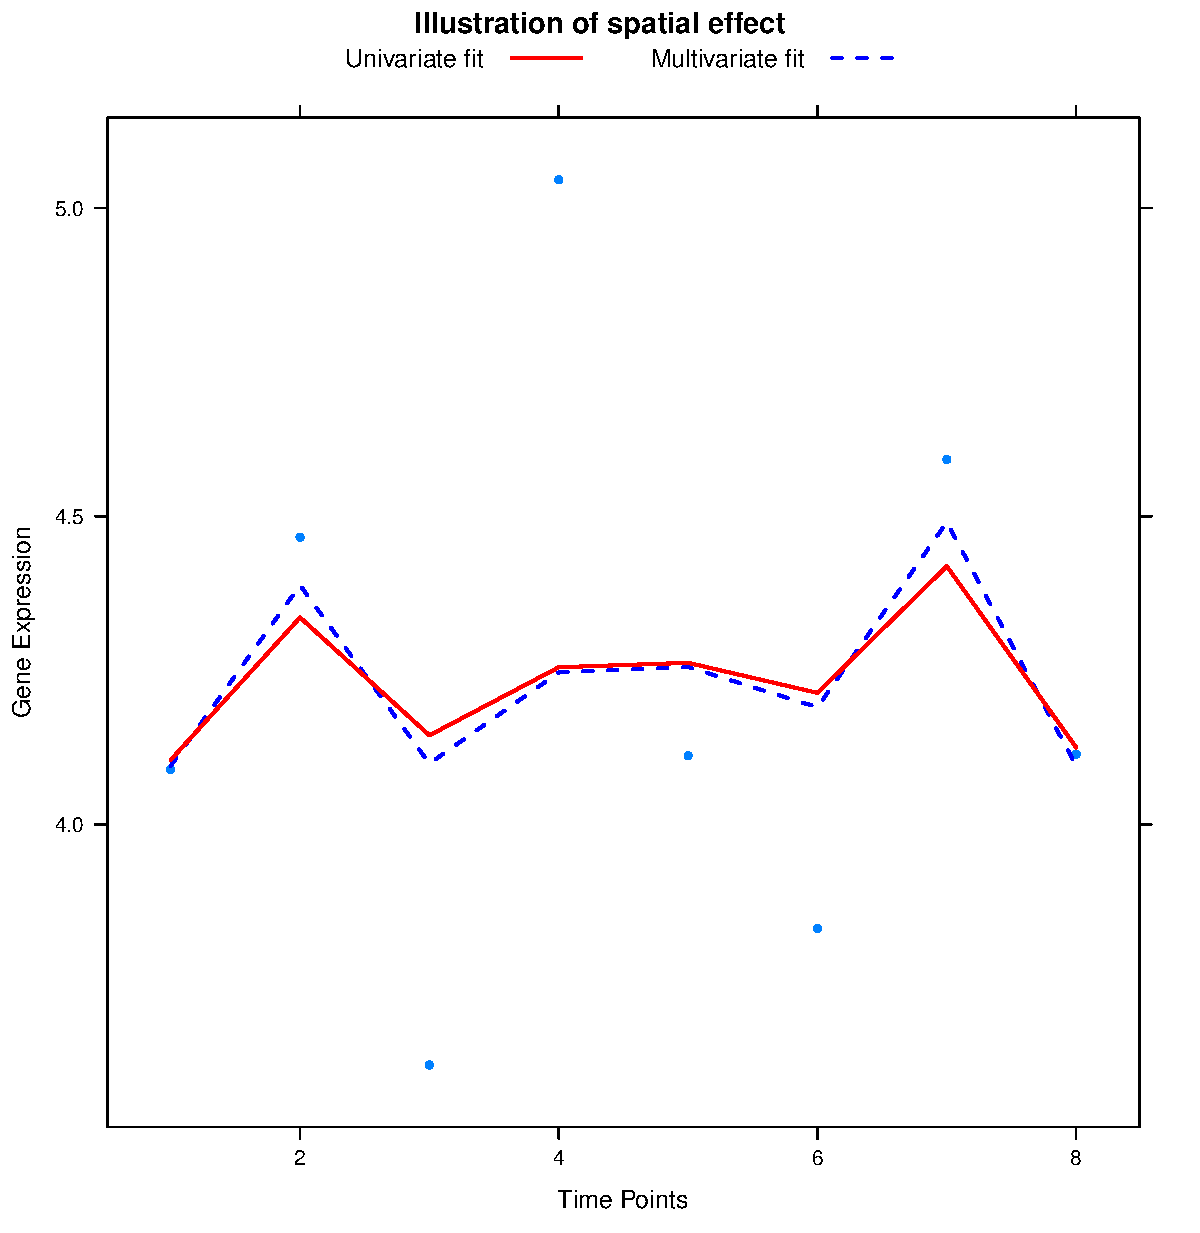
\includegraphics[scale=0.65]{Figure2.pdf}
\end{tabular}
\caption{Technical validation of microarray results by qRT-PCR for \textbf{A} mRNAs DEK, DKK3, SLC25A36 and \textbf{B} miRNAs miR-100-5p, miR-103a-3p, miR-125b-5p, miR-15b-5p and miR-221-5p. The Spearman correlation coefficient (Rho) and associated p-value (p) are indicated.}
\label{fig:figure52}
\end{figure}
\\
\\
\textbf{Validation of differential gene expression in cervical tissue samples}
\\
To investigate the in vivo relevance of our findings, expression patterns of 39 out of 106 differential miRNAs and 2661 out of 3642 differential mRNAs could be obtained from in-house available microarray data of normal HPV-positive cervical epithelium, high-grade precancerous lesions (CIN2/3) and squamous cell carcinomas (SCC, \cite{Wilting2013} and unpublished data). A concordant significant pattern of up- or downregulation was observed from normal to CIN to SCC by Spearman correlation for 24$\%$ of investigated mRNAs and 49$\%$ of investigated miRNAs. No significant up- or downward trend was observed for 62$\%$ of mRNAs and 33$\%$ of miRNAs, whereas 15$\%$ of mRNAs and 18$\%$ of miRNAs showed an opposite expression pattern in tissues compared to the cell line model.
Figure \ref{fig:figure55} shows ID1 and PITX2 as examples for mRNAs with increased or decreased expression, respectively. Deregulated miRNAs are represented by miR-4284-5p and miR-218-5p. For PITX2 and miR-4284-5p a copy number effect can be observed (fitted model with copy number effect).
\begin{figure}[h!]
\centering
\begin{tabular}{cc} 
\includegraphics[scale=0.6]{Figure5.pdf}
\end{tabular}
\caption{Deregulated mRNAs and miRNAs. Representative mRNAs (ID1, PITX2) and miRNAs (miR-4284, miR-218-5p) for increased and decreased expression are shown. Fitted models represent curves obtained using methodology from \cite{Miok2014}. If red and blue lines are similar (ID1, miR-218-5p), there is no effect of copy number on gene expression.
}
\label{fig:figure55}
\end{figure}
\\
\\
\textbf{Pinpointing key regulators in enriched pathways}
\\
Based on the unsupervised hierarchical cluster results we hypothesized that a substantial proportion of the above described DNA copy number induced gene expression changes are involved in the acquisition of anchorage independence. Indeed, 3 of the most significantly overrepresented pathways among all DNA copy number associated genes (Table \ref{table:table4}), focal adhesion, TGF-$\beta$ and mTOR signalling, are implicated in processes underlying anchorage independence (i.e. anoikis resistance and induction of EMT) \cite{Paoli2013, Frisch2013}. To further investigate this we translated our longitudinal data into pathway-based networks for focal adhesion (KEGG hsa04510), TGF-$\beta$ signalling (KEGG hsa04350) and mTOR signalling (KEGG hsa04150) (Table \ref{table:table4} and Materials $\&$ Methods section). Data-driven longitudinal networks were built for all genes in the respective pathways taking copy number into account and key regulators were identified for all 3 pathways (Table \ref{table:table2}, Figure \ref{fig:figure53}).%, Suppl. Table 5).
\begin{figure}[h!]
\centering
\begin{tabular}{cc} 
\includegraphics[scale=0.65]{Figure3.pdf}
\end{tabular}
\caption{Networks of the \textbf{A} focal adhesion, \textbf{B} mTOR signalling, and \textbf{C} TGF-$\beta$ signalling pathways. Nodes represent the genes, while the lines interaction among the genes at different time point. Dashed lines represent negative effect, while solid lines positive effect. The $X_t$ indicate copy number effect measured at time point $t$, while $Y_t$ and $Y_{t+1}$ gene expression at current and next time point.}
\label{fig:figure53}
\end{figure}
\\
\\
\textbf{Identification of potential miRNA-mRNA target interactions}
\\
Using our developed {\tt tigaR} framework we were also able to further investigate the relation between miRNA and mRNA expression in a longitudinal fashion. For this analysis we focused on the 86 miRNAs for which altered expression was either validated or not measured in the tissue specimens (excluding 20 miRNAs with non-significant changes or opposite changes in tissues). For 44 miRNAs no significant associations were found with any of the mRNA genes, whereas an additional 3 miRNAs were only displaying positive associations. When restricting the analysis to miRNA-mRNA pairs showing significant changes in expression over time in the opposite direction, 634 interactions between 27 miRNAs and 372 mRNAs remained. To verify these 634 potential interactions, we used 3 up-to-date publicly available target prediction databases ((RNA22 v2.0 \cite{Miranda2006}, miRDB v5 \cite{Wong2015}, and TargetScan v7 \cite{Agarwal2015}). Four interactions were predicted by all 3 databases (Table \ref{table:table3}), 61 interactions were predicted twice, and 225 interactions were predicted once, whereas the remainder (344 interactions) were not predicted by any of the databases. %(Suppl. Table 6). 

\begin{table}[htbp]
  \centering
  \caption{Top four predicted interactions of down-regulated miRNA and up-regulated mRNA, using data bases TargetScan\_v7, miRDB\_v5, RNA22 v2.0. Last column represent counts, number of data bases where interactions are predicted.}
    \begin{tabular}{lcccccc}
   \hline
    \hline
    \textbf{Pred. interactions} & \textbf{miR} & \textbf{mRNA} & \textbf{TargetScan} & \textbf{miRDB} & \textbf{RNA22} & \textbf{Ct} \\
    \hline
    miR-221-3p\_BRWD3 & down  & up    & target & target & target & 3 \\
    miR-221-3p\_FOS & down  & up    & target & target & target & 3 \\
    miR-30a-3p\_PECR & down  & up    & target & target & target & 3 \\
    miR-138-5p\_PLXNB2 & down  & up    & target & target & target & 3 \\
    \hline
    \hline
    \end{tabular}%
  \label{table:table3}%
\end{table}%

We selected one of the four 3 times predicted interactions, miR-221-3p\_BRWD3, for further functional validation, since miR-221-3p is known for its dual role in cancer as oncomiR and tumor suppressor miRNA \cite{Garofalo2012} and upregulation of the chromatin modifier BRWD3 was observed in cervical precancerous lesions and SCCs as well as in our model system \cite{Boon2015}. Ectopic overexpression of the miR-221-3p in late FK18B cells ($\sim$ passage 190) resulted in a 40$\%$ reduction of BRWD3 expression (Figure \ref{fig:figure54}A). As is shown in Figure \ref{fig:figure54}B, co-transfection of pmiRGLO\_BRWD3\_3UTR and ectopic miR-221-3p in Hek293 cells decreased luciferase activity compared to either co-transfection of pmiRGLO\_BRWD3\_3UTR with a non-targeting control sequence or the empty pmiRGLO vector with ectopic miR-221-3p. Directed mutagenesis of the predicted miR-221-3p seed sequence (pmiRGLO\_BRWD3\_3UTR-mut) abolished the reduction in luciferase activity observed with the wild type vector.

\begin{figure}[h!]
\centering
\begin{tabular}{cc} 
\includegraphics[scale=0.6]{Figure4.pdf}
\end{tabular}
\caption{\textbf{A} Effect of miR-221-3p on BRWD3 mRNA levels as determined by qRT-PCR in late FK18B cells (ca. passage 190). Mimic control 2 (cntr$\#$2) was used as negative transfection control, data was normalized to snRNP U1A. \textbf{B} Dual-luciferase reporter assay in Hek293 cells transiently transfected with a ne negative control (cntr$\#$1) or miR-221-3p in combination with either an empty pmiRGLO vector, a pmiRGLO-BRWD3-3UTR construct or a pmiRGLO-BRWD3-3UTR construct with mutated binding site of miR-221-3p (pmiRGLO-BRWD3-3UTR\_mut).}
\label{fig:figure54}
\end{figure}

\section{Discussion}

We here present one of the most extensive studies characterizing HPV-induced transformation over time. Chromosomal, mRNA and miRNA expression profiles were obtained from 4 individual HPV-transformed keratinocyte cell lines at 8 different time points. The obtained unique longitudinal multi-level dataset allowed for the identification of key regulators of disturbed pathways and the detection of miRNA-mRNA interactions in HPV-induced transformation. Importantly, HPV-transformed keratinocytes have previously been shown to provide useful model systems to study chromosomal instability in cancer in general \cite{Korzeniewski2011, Duensing2002}, indicating that insights on the sequential order of crucial molecular events gained in HPV-induced transformation might not only provide a better understanding of cervical cancer development, but could be applicable to other cancers too. 

Contrary to previous reports, we found that approximately one third of expression changes were directly associated to copy number, irrespective of RNA class (mRNA or miRNA) investigated. Medina-Martinez et al. found that 12.0$\%$ (241 out of 2010) differentially expressed mRNAs were related to copy number in HPV16-positive cervical tissue samples and in our cervical tissue data only a small minority of differentially expressed miRNAs was linked to copy number (5 out of 106 = 4.7$\%$) \cite{Wilting2013, Kanehisa2000, Miok2017, Livak2001, Wilting2016, Paoli2013, Frisch2013, Garofalo2012, Boon2015, Korzeniewski2011, Duensing2002, Medina2014}. Moreover, the expression of only 2 miRNAs was influenced by copy number in hematopoietic cell lines, suggesting that there is little correlation between copy number and miRNA expression \cite{Veigaard2014}. On the other hand, \cite{Zhang2006} identified 41 miRNA genes with copy number changes that were shared between melanoma, ovarian and breast cancer and many more miRNA genes with copy number changes that were unique to each of the epithelial tumor types \cite{Zhang2006}. In accordance with our data, copy number losses were reported to account for the down-regulation of approximately 15$\%$ of miRNAs in advanced ovarian tumors \cite{Zhang2008}. Discrepancies between studies can be explained by the multitude of different experimental approaches and statistical methods used to study the association between copy number and miRNA expression. While most studies analyzed cross-sectional clinical material or a number of cell lines, we here had the unique opportunity to follow copy number and gene expression changes within the specific cellular background of our 4 transforming cell lines over time. In addition, we cannot exclude that the large fraction of copy number induced expression changes found in our study is specific to cervical carcinogenesis and that copy number changes might have less impact on mRNA and miRNA expression in a different context.

Besides studying the effect of copy number aberrations on gene expression, our previously developed {\tt tigaR} framework also proved suitable for the identification of miRNA-mRNA interactions\cite{Miok2014}. We identified a total of 634 potential miRNA-mRNA interactions and validated the miR-221-3p\_BRWD3 interaction on RNA level and by dual-luciferase assay. 

As described before unsupervised hierarchical clustering of our miRNA expression data separated well between anchorage-dependent and independent passages of our transformed keratinocyte cell lines \cite{Wilting2016}, but the role of chromosomal alterations in the acquisition of anchorage independence was even more eminent. Anchorage-independent cell growth is a hallmark of transformation in vitro \cite{Freedman1974, Mori2009}. While loss of appropriate cell-cell and cell-matrix interactions leads to aberrant integrin signalling and eventually detachment-induced cell death (anoikis) in healthy epithelial cells, cancerous epithelial cells overcome anoikis by epithelial-to-mesenchymal transition (EMT), activation of survival and proliferation pathways or temporary dormancy \cite{Guadamillas2011}. In HPV-transformed cells, silencing of a number of tumour suppressor genes (including miRNAs) was shown to contribute to anchorage-independence \cite{Wilting2016, Khalifa2011, Mack2013, Overmeer2009, Razani2000, Steenbergen2004}). Our clustering results suggest that anchorage-independent cell growth represents highly relevant functional read-out when studying the effect of molecular changes on transformation in vitro.

Pathway enrichment analysis on copy number affected mRNAs identified focal adhesion, mTOR signalling and TGF-$\beta$ signalling as the top 3 altered pathways in HPV-induced carcinogenesis. Strikingly, all 3 pathways are implicated in anoikis resistance and induction of EMT \cite{Paoli2013, Frisch2013, Garofalo2012}, again suggesting that the acquisition of anchorage independence in HPV-induced transformation is largely driven by chromosomal changes. It is therefore not surprising that extracellular matrix proteins such as LAMA4 (laminin subunit alpha 4), COL5A3 (collagen type V alpha 3) and motor protein MYLPF (myosin light chain, phosphorylatable, fast skeletal muscle) were among the key regulators of focal adhesion signalling. Consistent with the here observed downregulation of LAMA4, it has previously been shown that ectopic overexpression of LAMA4 resulted in increased cellular adhesion in anchorage-independent cervical cancer cell line HeLa54. Similarly, the here identified key regulators of the mTOR pathway IGF1 (insulin like growth factor 1) and HIF1A (hypoxia inducible factor 1 alpha subunit) were previously described to be involved anoikis resistance in hepatocellular carcinoma cells \cite{Tang2015, Sun2014}. HIF1A also upregulates EMT inducers such as SNAI1, TWIST and SIP1 \cite{Luo2011, Yang2008, Evans2007}). TGF-$\beta$1 has been reported to exert a tumor inhibiting function in early stages of cervical carcinogenesis, while it plays an oncogenic role at a later stage by promotion of EMT and metastasis, induction of angiogenesis and escape from immune surveillance \cite{Zhu2016}. In line with this, expression of TGF-$\beta$1 was found to be downregulated in cervical precancerous lesion compared to normal epithelium although it is increased in cervical cancers \cite{Wu2002, Hou2012, Fan2014}. This TGF-$\beta$ paradox is not unique to cervical carcinogenesis but has been recognized in many other cancers as well \cite{Massague2008, Neuzillet2015, Shen2017}. A number of TGF-$\beta$ and TGF-$\beta$ receptor inhibitors is currently being tested for the treatment of a variety of cancers in phase I-IV clinical trials \cite{Colak2017}. In cervical cancer, a negative correlation between pre-radiation TGF-$\beta$1 levels and radiosensitivity suggests that tumor response can be increased by inhibition of TGF-$\beta$1 prior to radiation \cite{Zhu2016}.

We here present a unique longitudinal multi-level dataset on HPV-induced transformation. Using state-of-the-art analysis tools, we identified key pathway regulators and potential miRNA-mRNA interactions relevant to the carcinogenic process. Our results highlight the importance of chromosomal alterations for the acquisition of anchorage independence during transformation. Additional functional studies on the identified key pathway regulators and differentially expressed m(i)RNAs will likely result in many more potential therapeutic targets and disease markers in the future.
\begin{table}[htbp]
  \centering
  \caption{Network enrichment analysis of copy number related genes in 118 KEGG pathways.}
    \begin{tabular}{lccc}
    \hline\hline
    & \multicolumn{1}{l}{\textbf{Nr. of }} & \multicolumn{1}{l}{\textbf{\% of CN      }} & \multicolumn{1}{l}{\textbf{Adj.}} \\
    \multicolumn{1}{c}{\textbf{keggName}} & \multicolumn{1}{l}{\textbf{genes in}} & \multicolumn{1}{l}{\textbf{related}} & \multicolumn{1}{l}{\textbf{P-value}} \\
    & \multicolumn{1}{p{3.89em}}{\textbf{pathway}} & \multicolumn{1}{p{4.39em}}{\textbf{genes}} & \multicolumn{1}{p{4.165em}}{\textbf{ (Chi2)}} \\
    \hline
    \rowcolor[rgb]{ 1,  1,  0}  Focal adhesion & 200   & 7.50  & 0.0001 \\
    \rowcolor[rgb]{ 1,  1,  0}  TGF-beta signaling pathway & 85    & 5.88  & 0.0152 \\
    \rowcolor[rgb]{ 1,  1,  0}  mTOR signaling pathway & 52    & 5.77  & 0.0268 \\
    Nucleotide excision repair & 45    & 4.44  & 0.0000 \\
    Mismatch repair & 23    & 4.35  & 0.0003 \\
    p53 signaling pathway & 69    & 4.35  & 0.0008 \\
    Wnt signaling pathway & 151   & 3.31  & 0.0018 \\
    Biosynthesis of unsaturated fatty acids & 21    & 4.76  & 0.0019 \\
    Neurotrophin signaling pathway & 127   & 3.15  & 0.0033 \\
    B cell receptor signaling pathway & 75    & 8.00  & 0.0036 \\
    Cell cycle & 128   & 7.81  & 0.0038 \\
    Glycosaminoglycan biosynthesis & 26    & 7.69  & 0.0242 \\
    Glycosylphosphatidylinositol(GPI) & 25    & 8.00  & 0.0242 \\
    N-Glycan biosynthesis & 49    & 6.12  & 0.0245 \\
    Purine metabolism & 162   & 4.32  & 0.0268 \\
    Glutathione metabolism & 50    & 8.00  & 0.0268 \\
    mRNA surveillance pathway & 83    & 0.00  & 0.0271 \\
    Synthesis and degradation of ketone bodies & 9     & 11.11 & 0.0311 \\
    Aminoacyl-tRNA biosynthesis & 63    & 3.17  & 0.0400 \\
    Thiamine metabolism & 4     & 0.00  & 0.0487 \\
    Lipoic acid metabolism & 3     & 0.00  & 0.0487 \\
    \midrule
    Apoptosis & 89    & 4.49  & 0.0542 \\
    Valine  leucine and isoleucine degradation & 44    & 2.27  & 0.0563 \\
    Alanine  aspartate and glutamate metabolism & 32    & 15.63 & 0.0606 \\
    T cell receptor signaling pathway & 108   & 6.48  & 0.0731 \\
     Pyrimidine metabolism & 99    & 2.02  & 0.0774 \\
     Porphyrin and chlorophyll metabolism & 43    & 4.65  & 0.0913 \\
    Phosphatidylinositol signaling system & 78    & 2.56  & 0.0913 \\
     Sphingolipid metabolism & 40    & 2.50  & 0.0913 \\
     Ribosome biogenesis in eukaryotes & 81    & 1.23  & 0.1173 \\
     Glycosphingolipid biosynthesis & 26    & 7.69  & 0.1373 \\
     ECM-receptor interaction & 85    & 7.06  & 0.1373 \\
    Fatty acid metabolism & 43    & 2.33  & 0.1451 \\
     ErbB signaling pathway & 87    & 3.45  & 0.1504 \\
     Inositol phosphate metabolism & 57    & 1.75  & 0.1942 \\
    \hline\hline
\end{tabular}%
  \label{table:table4}%
\end{table}%


\chapter{Aberrant methylation-mediated silencing of microRNAs contributes to HPV-induced anchorage independence \\ {\footnotesize (\textit{Wilting, S. M., Miok, V., Jaspers, A., Boon, D., Sorgard, H., Lando, M., Snoek, B. C., van Wieringen, W. N., Meijer, C.J.L.M., Lyng, H., Snijders, P.J.F., Steenbergen, R.D.M., Oncotarget (2016), 7(28): 43805-43819})}}
\chaptermark{HPV-induced anchorage independence}
\label{chapter:Window estimator}

\graphicspath{{Chapte6/Figs/}{Chapter6/Figs/PDF/}{Chapter6/Figs/}}%

Cervical cancer and a subset of anogenital and head-and-neck carcinomas are caused by high-risk types of the human papillomavirus (hrHPV). During hrHPV-induced malignant transformation keratinocytes become able to grow anchorage independently, a tumorigenic trait at least partly associated with inactivation of tumor suppressor genes. We used hrHPV-containing keratinocytes to investigate the role of DNA methylation-mediated silencing of microRNAs (miRNAs) in the acquisition of anchorage independence.

Anchorage dependent (n=11) and independent passages (n=19) of 4 hrHPV-immortalized keratinocyte cell lines were treated with 2'-deoxy-5-azacytidine (DAC). Genome-wide miRNA expression profiles before and after treatment were compared to identify miRNAs silenced by methylation. Bisulfite sequencing and methylation-specific PCR showed increased methylation of hsa-mir-129-2/-137/-935/-3663/-3665 and -4281 in anchorage independent HPV-transformed keratinocytes and cervical cancer cell lines. Mature miRNAs derived from hsa-mir-129-2/-137/-3663 and -3665 showed functional relevance as they decreased anchorage independence in cervical cancer cell lines. Cervical (pre)cancerous lesions demonstrated increased methylation of hsa-mir-129-2/-935/-3663/-3665 and -4281, underlining the clinical relevance of our findings.  

In conclusion, methylation-mediated silencing of tumor suppressive miRNAs contributes to acquisition of an anchorage independent phenotype. This study further substantiates the importance of miRNAs during early stages of carcinogenesis and underlines their potential as both disease markers and therapeutic targets.
\\
\\
This chapter corresponds to the article:\\
 Wilting, S. M., Miok, V., Jaspers, A., Boon, D., Sorgad, H., Lando, M., Snoek, B. C., van Wieringen, W. N., Meijer, C. J. L. M., Lyng H., Snijders, P. J. F. and Steenbergen, R. D. M. (2016). Aberrant methylation-mediated silencing of microRNAs contributes to HPV-induced anchorage independence. \textit{Oncotarget}, 7(28): 43805-43819.

\section{Introduction}

Persistent infection with high-risk types of the human papillomavirus (hrHPV) is causally related to virtually all cervical cancers as well as a subset of other anogenital and head and neck carcinomas. 

Normally, the viral life cycle of HPV is tightly linked to differentiation of the infected epithelium, resulting in very low expression of the viral oncogenes E6 and E7 in the basal dividing cells. In so-called transforming infections deregulated expression of E6 and E7 is found in the dividing cells. This aberrant expression results in uncontrolled cell proliferation and subsequent genetic instability. The latter is considered a driver of further cellular transformation \cite{Doorbar2006}. Previous studies in which primary keratinocytes were transfected with either full length hrHPV types or with the viral oncogenes E6/E7 showed that hrHPV-induced transformation involves 4 distinct phenotypic stages: extended life span, immortality, anchorage independence and tumorigenicity \cite{Chen1993, Schutze2014}.

Anchorage independent growth is considered a crucial step in carcinogenesis and is often considered as surrogate marker for complete transformation in vitro \cite{Freedman1974, Mori2009}. Epithelial cells are dependent on proper cell-cell and cell-matrix interactions (“anchors”) for both differentiation and proliferation. Loss of these interactions results in aberrant integrin signaling and subsequent induction of anoikis (detachment-induced cell death). Cancerous epithelial cells were shown to use various strategies to circumvent anoikis, including adaptation to the new environment by epithelial-to-mesenchymal (EMT) like de-differentiation or integrin switching, constitutive activation of survival and proliferation pathways, and temporary dormancy through either autophagy or entosis (reviewed by \cite{Guadamillas2011}). Cell fusion studies have shown that anchorage independence of hrHPV-transformed cells relies on a recessive event, suggesting that inactivation of tumor suppressor genes is involved in bypassing anoikis \cite{Chen1993}. In support of this, functional loss of tumor suppressive host genes Caveolin-1, SOCS1, TAp63$\beta$, LKB1, CADM1, MAL, hsa-miR-34c-3p/5p and hsa-miR-203 was shown to affect anchorage independent growth of HPV-transformed cells \cite{Khalifa2011, Kamio2004, Mack2013, Overmeer2009, Razani2000, Steenbergen2004, Wilting2013,Lopez2011}. 

Epigenetic changes, represent an important mechanism for the silencing of tumor suppressor genes. In cervical cancer, DNA methylation-mediated silencing of a rapidly growing number of coding and non-coding genes is being found and functional relevance has been demonstrated for part of these genes \cite{Steenbergen2014, Szalmas2009, Wentzensen2009}. In cervical cancer increased methylation has been shown for a number of miRNAs, including hsa-mir-34b, -95, -124, -125b1, -149, -203, -214, and -375 \cite{Wilting2013, Botezatu2011, Soto2012, Wang2013, Wilting2010, Yao2013, Zhu2013}. However, so far a systematic investigation of the involvement of aberrantly methylated miRNAs in hrHPV-induced transformation is lacking. 

In this study we used a well characterized in vitro model system consisting of 4 hrHPV-containing keratinocyte cell lines to thoroughly investigate the contribution of DNA methylation-mediated silencing of miRNAs to hrHPV-mediated transformation \cite{Steenbergen1996}. To this end genome-wide miRNA expression profiles were generated during different stages of transformation with and without demethylating 2'-deoxy-5-azacytidine (DAC) treatment. To select miRNAs (potentially) silenced by methylation, DAC-induced fold changes in mature miRNA expression were combined with DNA methylation levels measured by Infinium HumanMethylation450 BeadChip. Bisulfite sequencing and methylation-specific PCR (MSP) analysis were performed to verify DNA methylation both in cell lines and cervical (pre)cancerous tissue specimens. In addition, for all miRNAs that showed increased DNA methylation during HPV-induced transformation we determined effects of their ectopic expression on viability and anchorage independence of cervical cancer cell lines SiHa and CaSki.
\begin{table}[htbp]
  \centering
  \caption{Passage numbers included for all 4 hrHPV-transformation cell lines. FK16A and FK16B contain HPV16, wheres FK18A and Fk18B contain HPV18. Grey shaded passages represent anchorage dependent cells, whereas non-shading passages are able to grow anchorage independently.}
    \begin{tabular}{ccccc}
    \hline\hline
    \textbf{Time point} & \textbf{FK16A } & \textbf{FK16B } & \textbf{FK18A } & \textbf{FK18B } \\
    \hline
    T1    & \cellcolor[rgb]{ .753,  .753,  .753}p18 & \cellcolor[rgb]{ .753,  .753,  .753}p21 & \cellcolor[rgb]{ .753,  .753,  .753}p19 & \cellcolor[rgb]{ .753,  .753,  .753}p17 \\
    T2    & \cellcolor[rgb]{ .753,  .753,  .753}p22 & \cellcolor[rgb]{ .753,  .753,  .753}p22 & \cellcolor[rgb]{ .753,  .753,  .753}p21 & \cellcolor[rgb]{ .753,  .753,  .753}p18 \\
    T3    & \cellcolor[rgb]{ .753,  .753,  .753}p39 & p45   & p47   & p40 \\
    T4    & \cellcolor[rgb]{ .753,  .753,  .753}p52 & p51   & p60   & p52 \\
    T5    & p109  & p89   & p92   & p90 \\
    T6    & p115  & p102  & p99   & p98 \\
    T7    & p206  & p140  & p148  & p146 \\
    T8    & p222  & p169  & p160  & p164 \\
    \hline\hline
    \end{tabular}%
  \label{table:table1}%
\end{table}%

\section{Results}

\textbf{Anchorage independence coincides with marked changes in overall miRNA expression}
\\
To study methylation-mediated silencing of miRNAs during HPV-induced transformation, we investigated 4 independent HPV-transformed keratinocyte cell lines at different stages during transformation. miRNA expression was determined in all 4 cell lines at 6-8 different passages (hereafter referred to as timepoints) with and without demethylating DAC treatment (Table \ref{table:table1}). First we determined whether the selected timepoints represent distinct stages during HPV-induced transformation. hTERT expression, reflecting telomerase activation, was detectable at all timepoints for FK16A, FK16B and FK18A, suggesting that cells at all timepoints were already immortal (Figure \ref{fig:figure1} A). In the first 2 timepoints of FK18B virtually no hTERT expression was detectable indicating these cells are still in their extended lifespan stage (Figure \ref{fig:figure1}A). These findings are in concordance with previous telomerase activity assays done on these cell lines \cite{Steenbergen1996}. From all 4 cell lines both anchorage dependent and anchorage independent (i.e. fully transformed) timepoints were included (Table \ref{table:table1} and Figure \ref{fig:figure1}A). Therefore our experimental set up allows further investigation of the contribution of methylation-mediated miRNA silencing to acquisition of anchorage independence. 

Interestingly, unsupervised clustering analysis of the baseline miRNA expression profiles (without DAC treatment) showed a clear distinction between anchorage dependent and anchorage independent timepoints in FK16A, FK16B and FK18B (Figure \ref{fig:figure1}B, \ref{fig:figure1}C and \ref{fig:figure1}E). The highest anchorage dependent timepoint (T3) of FK18A clustered together with subsequent anchorage independent timepoints, suggesting that these FK18A T3 cells were on the verge of anchorage independence (Figure \ref{fig:figure1}D). The stability of the clustering patterns was corroborated by consensus clustering \cite{Monti2003}. These results indicate that changes in miRNA expression are associated with the acquisition of anchorage independence.  
\\
\\
\textbf{Identification of miRNAs silenced by methylation during HPV-induced transformation}
\\
Next we compared miRNA expression between DAC treated and untreated cells of all timepoints per cell line. Figure \ref{fig:figure2} summarises the selection procedure we used to identify the most promising methylation candidates. 

  In total 104 CpG-island associated miRNA genes (as defined in Materials $\&$ Methods) encoding 126 mature miRNAs were included in the analysis. Per cell line we selected 1) the 25 miRNAs showing the highest upregulation upon DAC treatment over all timepoints and 2) the 25 miRNAs with the highest upregulation in anchorage independent timepoints. The resulting lists of candidate miRNAs were compared between the 4 cell lines and miRNAs were selected for further investigation if they were identified in 2 or more cell lines. This was the case for  57 mature miRNAs corresponding to 45 miRNA genes. An additional 16 mature miRNAs were only selected in 1 of the 4 cell lines and were therefore discarded from further analysis ( \cite{Supp2018} Table 6.1.).

  DNA methylation was measured for 40 of the 45 selected miRNA gene loci in primary keratinocytes (HFK) of 2 donors, FK16A T8, FK16B T7, FK18A T6 and FK18B T7 (all anchorage independent) using an Infinium HumanMethylation450 BeadChip. Genes showing 1) low methylation levels in primary keratinocytes (<25$\%$), 2) at least 50$\%$ methylation in (part of) the HPV-transformed keratinocytes, and 3) a minimal increase in methylation of 30$\%$ from primary keratinocytes to HPV-transformed keratinocytes, were selected. In addition, we also selected the 5 miRNA genes for which no probes were available on the BeadChip. This resulted in selection of the following 10 miRNA genes for further investigation: hsa-mir-129-2, -137, -615, -675, -935, -2277, -3663, -3665, -4281, and -4323.
\begin{figure}[h!]
\centering
\begin{tabular}{cc} 
\includegraphics[scale=2.5]{Figure1.jpg}
\end{tabular}
\caption{Characterisation of our longitudinal in vitro model system of hrHPV-induced transformation. In A. anchorage dependent (grey) and independent (white) timepoints (T) of all 4 cell lines are shown in relation to the transformation process. Unsupervised hierarchical cluster results based on overall miRNA expression are shown for B. FK16A, C. FK16B, D. FK18A, and E. FK18B. Anchorage dependent timepoints are marked in grey, whereas anchorage independent timepoints are white. }
\label{fig:figure1}
\end{figure}
\\
\\
\textbf{Bisulfite sequencing analysis of the regulatory sequences of selected miRNA genes}
\\
Bisulfite sequencing was performed on HFKs, anchorage independent HPV-transformed keratinocytes (FK16/18A/B), and cervical cancer cell lines (SiHa, HeLa or CaSki). For all 10 selected miRNA genes a region between 1000-500bp directly upstream of the transcription start site (TSS) was sequenced. Differential methylation in HPV-transformed keratinocytes and cancer cell lines compared to HFK was observed for hsa-mir-129-2, -137, -935 -3663, -3665, and -4281 (Figure \ref{fig:figure3}A, B, E, G, H, and I, respectively). For hsa-mir-615 methylation was only observed in cervical cancer cells and not in HPV-transformed keratinocytes (Figure \ref{fig:figure3}C), suggesting this to be a late event. No methylation was observed upstream of hsa-mir-2277 in any of the cells tested (Figure 3F). On the other hand, methylation upstream of hsa-mir-675 and -4323 was already observed in primary keratinocytes without HPV (Figure \ref{fig:figure3}D and J). Based on these results, hsa-mir-675, -2277, and -4323 were excluded from further analyses. 
\begin{figure}[h!]
\centering
\begin{tabular}{cc} 
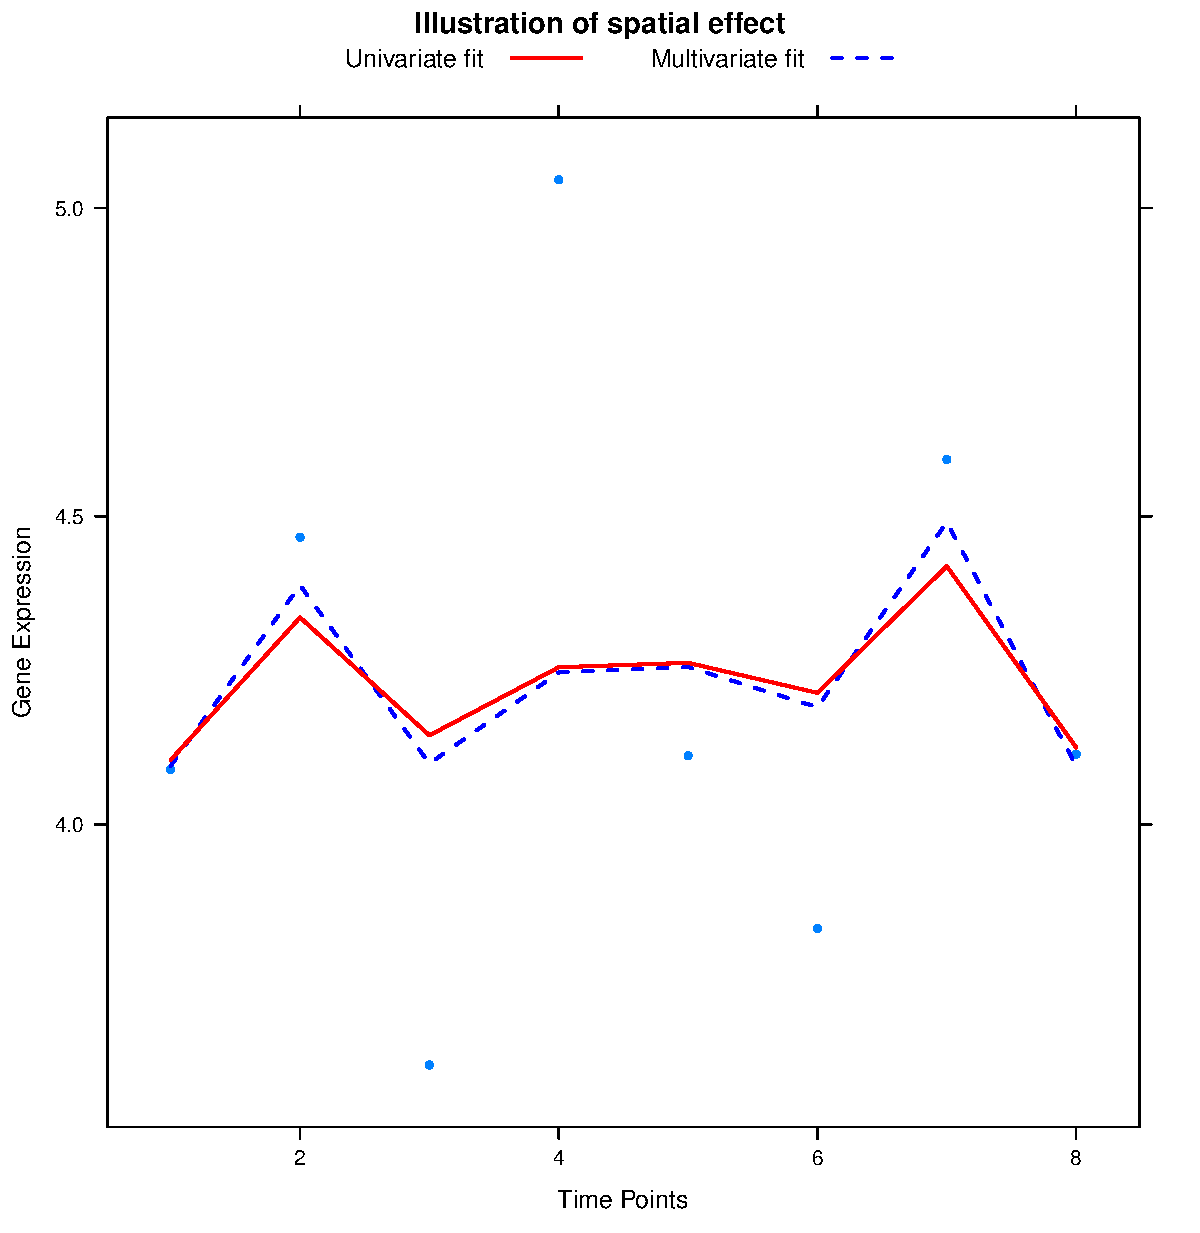
\includegraphics[scale=3]{Figure2.jpg}
\end{tabular}
\caption{Schematic overview of the analysis pipeline used to select the most promising potential methylation targets.}
\label{fig:figure2}
\end{figure}
\\
\\
\textbf{Aberrant hsa-mir-129-2, -137, -935, -3663, -3665, and -4281 methylation is common in HPV-transformed cells}
\\
To allow sensitive methylation analysis in larger numbers of samples, methylation-specific PCR (MSP) assays were designed for hsa-mir-129-2, -137, -615, -935, -3663, -3665, and -4281. Using the sequencing data described above we specifically designed primers to target the most differentially methylated region close to the TSS of the miRNA genes (indicated with grey arrows in Figure \ref{fig:figure3}). MSP was performed on HFKs of 3 independent donors, anchorage independent passages of all 4 HPV-transformed keratinocyte cell lines (FK16A, FK16B, FK18A and FK18B) and the cervical cancer cell lines SiHa, HeLa, and CaSki (Figure \ref{fig:figure4}). For hsa-mir-129-2 and -3663 no methylation was observed in any of the HFKs, whereas all HPV-transformed keratinocytes and cervical cancer cell lines showed clear methylation (Figure 4A and E). Concordant with sequencing results, methylation for hsa-mir-615 was only observed in the cervical cancer cell lines (Figure \ref{fig:figure4}C and \ref{fig:figure3}C). For hsa-mir-137, -935, -3665, and -4281 low levels of methylation were observed in part of the primary keratinocytes, but methylation clearly increased in most HPV-transformed keratinocytes and cervical cancer cell lines. The fact that with sequencing no methylation was observed for these miRNAs in HFK (Figure \ref{fig:figure3}B, E, H and I) is probably due to the higher analytical sensitivity of MSP compared to sequencing \cite{Eads2000, Kristensen2009}.  These results show that hsa-mir-129-2, -137, -935, -3663, -3665, and -4281 become hypermethylated during HPV-induced transformation. Methylation of hsa-mir-615, on the other hand, was only observed in cervical cancer cells and therefore does not seem to contribute to the process of transformation.
\begin{figure}[h!]
\centering
\begin{tabular}{cc} 
\includegraphics[scale=3.2, angle =270]{Figure3.jpg}
\end{tabular}
\caption{Bisulfite sequencing results of selected genomic regions in primary keratinocytes (HFK), HPV-transformed keratinocytes and cervical cancer cells. Results are shown for A. hsa-mir-129-2, B. hsa-mir-137, C. hsa-mir-615, D. hsa-mir-675, E. hsa-mir-935, F. hsa-mir-2277, G. hsa-mir-3663, H. hsa-mir-3665, I. hsa-mir-4281, and J. hsa-mir-4323. Methylation-independent sequencing primers are indicated by black arrows and methylation-specific MSP primers are indicated by grey arrows. TSS; transcription start site.}
\label{fig:figure3}
\end{figure}
\\
\\
\textbf{miRNA silencing by DNA methylation contributes to anchorage independent growth}
\\
Next, we investigated whether silencing of the identified six hypermethylated miRNA genes contributes to the ability to grow anchorage independently. For this purpose the corresponding mature miRNAs from the DAC screen were ectopically expressed in SiHa and CaSki cells, both of which were methylated for all six miRNA genes (Figure \ref{fig:figure3}). Successful transfection of all mimics was verified by (quantitative) RT-PCR (data not shown). Subsequently effects on cell viability (Figure \ref{fig:figure5}A) and anchorage independence were determined (Figure \ref{fig:figure5}B). Based on the variation observed between replicate control experiments, only effects larger than 30$\%$ compared to the control transfected cells were considered true effects. miR-129-2-3p and -137 reduced both cell viability and anchorage independence in both cell lines tested. miR-4281 did not show any effect on viability and anchorage independence in either cell line. miR-129-5p reduced viability in both cell lines whereas anchorage independence was only reduced by this miRNA in SiHa. miR-3663-3p and -3665 modestly reduced viability and anchorage independence in CaSki but not in SiHa cells. However, a borderline reduction in anchorage independence was observed in SiHa cells as well. Finally, miR-935 modestly reduced viability in SiHa but not in CaSki cells. Together, these results support the functional relevance of methylation-mediated silencing of miRNAs for HPV-induced transformation.
\begin{figure}[h!]
\centering
\begin{tabular}{cc} 
\includegraphics[scale=2.5]{Figure4.jpg}
\end{tabular}
\caption{MSP results for selected miRNA genes in 3 cervical cancer cell lines (SiHa, HeLa, CaSki), primary keratinocytes (HFK) of 3 independent donors, and anchorage independent passages of 4 HPV-transformed keratinocytes cell lines (FK16A, FK16B, FK18A, and FK18B). Results are shown for A. mir-129-2, B. mir-137, C. mir-615, D. mir-935, E. mir-3663, F. mir-3665, G. mir-4281, and H. ACTB (reference gene). In vitro methylated DNA (IVD) and unmodified DNA were included as positive and negative controls, respectively.}
\label{fig:figure4}
\end{figure}
\\
\\
\textbf{Increased methylation of hsa-mir-129-2, -935, -3663, -3665, and -4281 in cervical (pre)cancers}
\\
To verify the clinical relevance of our findings, methylation of mir-129-2, -137, -935, -3663, -3665 and -4281 was quantitatively determined in tissue specimens of normal cervical epithelium (n=22), CIN3 lesions (n=23), and SCCs (n=28). A significant increase in methylation levels with disease severity was observed for hsa-mir-129-2, -935, and -3663 (Figure \ref{fig:figure6}A, C and D). For mir-4281 the increase in methylation from normal to CIN3 lesions was only borderline significant (p =0.059) but a significant increase was seen in SCCs compared to both normal and CIN3 samples (Figure \ref{fig:figure6}F). Methylation of mir-3665 was absent in the large majority of samples but still showed a significant increase in SCCs (Figure \ref{fig:figure6}E). On the other hand, hsa-mir-137 showed relatively high methylation levels in all samples with a small, non-significant, increase in SCCs (p=0.089). 
In summary, methylation of hsa-mir-129-2, -935, -3663, -3665 and -4281 increases with disease severity in cervical tissue specimens. 
\begin{figure}[h!]
\centering
\begin{tabular}{cc} 
\includegraphics[scale=2.5]{Figure5.jpg}
\end{tabular}
\caption{Functional effects of miRNAs silenced by methylation on HPV-induced transformation. Effects of ectopic expression of mimics of all mature miRNAs derived from the methylated gene loci that showed a DAC effect (miR-129-5p, -129-2-3p, -137, -935, -3663, -3665, and -4281) were determined on A. cell viability and B. anchorage independent growth. Dashed lines indicate the threshold of 30$\%$ we used to discriminate true effects from random variation. Results are representative of 2 independent experiments.}
\label{fig:figure5}
\end{figure}

\begin{figure}[h!]
\centering
\begin{tabular}{cc} 
\includegraphics[scale=2.5]{Figure6.jpg}
\end{tabular}
\caption{Methylation levels of selected miRNA genes relative to the reference gene (ACTB) in normal cervical tissue specimens (n=22), CIN3 lesions (n=23) and SCCs (n=28).  Results are shown for A. hsa-mir-129-2, B. hsa-mir-137, C. hsa-mir-935, D. hsa-mir-3663, E. hsa-mir-3665, and F. hsa-mir-4281. ** indicates a two-sided p-value <0.001 (non-parametric Wilcoxon rank test).}
\label{fig:figure6}
\end{figure}

\section{Discussion}

This study systematically investigated the contribution of methylation-mediated silencing of miRNAs to hrHPV-induced transformation over time. Using an unbiased longitudinal approach, we identified 6 miRNA genes showing progressive silencing by methylation during HPV-induced transformation (hsa-mir-129-2, -137, -935, -3663, -3665, and -4281). Mature miRNAs derived from hsa-mir-129-2, -137, -3663, and -3665 reduced cell viability and/or anchorage independent growth to various extents in SiHa and CaSki cervical cancer cells. 

Unsupervised hierarchical clustering showed for the first time that anchorage dependent and anchorage independent timepoints within the same cell line could be discriminated based on their basal miRNA expression profiles. These clustering results suggest that alterations in miRNA expression are strongly associated with anchorage independent growth.

According to our definition only around 10$\%$ of the mature miRNAs measured were considered to come from CpG-island associated miRNA genes. This stringent definition limited the number of miRNAs included in the analysis. However, it was shown that in general DNA methylation in the region directly surrounding the TSS is most strongly associated with transcriptional silencing \cite{Brenet2011}. We were able to validate methylation for 2/3rd of genes showing strong DAC-induced re-expression. The majority of these genes were already methylated in primary keratinocytes, a phenomenon observed by Lujambio et al as well \cite{Lujambio2008}. 

Methylation of hsa-mir-129-2 has been described before in gastric, colorectal, renal, kidney, hepatocellular, esophageal, and endometrial carcinomas as well as in osteosarcomas \cite{Anwar2013, Bandres2009, Chen2012, Chen2013, Huang2009, Long2015, Lu2013, Shen2010, Tsai2011}. Interferon-$\beta$ dependent induction of hsa-miR-129-5p in cervical cancer cells was shown to reduce E6 and E7 expression via targeting of SP1 \cite{Zhang2013}. Additional targets described for hsa-miR-129-5p include SOX4, GALNT1, and VCP \cite{Chen2013, Huang2009, Long2015, Shen2010}. Hsa-miR-129-2-3p, which strongly reduced anchorage independence as well, was previously shown to reduce the levels of phosphorylated FAK protein and MMP2 and 9 proteins in renal carcinoma cells \cite{Chen2014}. Interestingly, altered activation of the FAK signaling pathway has previously been described in HPV-immortalized keratinocytes and cervical cancer cell lines and was linked to invasion and anchorage independence \cite{McCormack1997, Schwock2009, Srivastava2015}. 

Methylation of hsa-mir-137 has been described in oral and other head-and-neck, lung, bladder, breast, gastric, and colorectal cancers, glioblastomas, and neuroblastomas \cite{Bandres2009, Balaguer2010, Bier2013, Chen2011, Du2012, Kozaki2008, Langevin2010, Langevin2011, Shimizu2013, Steponaitiene2015, Takwi2014, Vrba2013, Wiklund2011}.  Remarkably, in our hands hsa-miR-137 strongly reduced viability and anchorage independent growth but did not show increased methylation in (pre)cancerous tissue biopsies. Tumor suppressive effects were described for hsa-miR-137 before \cite{Balaguer2010, Kozaki2008} and in other cancer types cancer-specific methylation of mir-137 was observed as well. However, also in these studies, differences between normal and cancer were small (on average $\sim$3x increase). Comparable to our results, also in these studies high background methylation was observed in normal samples \cite{Balaguer2010, Steponaitiene2015, Wiklund2011}. Described targets of hsa-miR-137 so far include CDK6, LSD1, RTVP1, CAR and CDC42 \cite{Balaguer2010, Bier2013, Kozaki2008, Takwi2014, Silber2008, Zhu2013}. Increased expression of CDC42 is found in cervical (pre)cancers and was shown to promote formation of filopodia/pseudopodia thereby facilitating migration, a phenotype associated with anchorage independence as well \cite{Ruiz2015, Ye2015}. 

To the best of our knowledge, methylation of the other miRNA genes identified in this study has not been described before. Hsa-miR-935 was shown to be downregulated in medulloblastoma \cite{Genovesi2011}, whereas hsa-miR-3663-3p and -4281 conversely were found upregulated in malignant melanoma \cite{Sand2013}. Hsa-miR-4281 and -935 did not influence anchorage independence, but they were specifically hypermethylated in (pre)cancers. Our results suggest that methylation of these miRNA genes is a relatively late event. Potentially, ectopic expression of these miRNAs therefore would have an influence on later phenotypes, such as invasion and tumorigenicity.   

Mature miRNAs derived from 4 out of 6 identified silenced miRNA genes reduced anchorage independent growth. This fact underlines the value of longitudinal in vitro model systems for the identification of (epi)genetic events that contribute to (HPV-induced) transformation. In addition, significantly increased methylation levels of hsa-mir-129-2, -935, -3663, -3665, and -4281 were observed in cervical high-grade precancerous lesions (CIN3) and SCCs compared to normal cervical epithelium as well. This underscores the clinical relevance of our in vitro findings. The methylation status of these genes in low-grade cervical lesions (CIN1) and the heterogeneous group of CIN2 lesions, believed to encompass both low-grade and high-grade cervical precancerous disease \cite{Wilting2016}, will be subject of future studies. In addition, these studies will address the potential marker value of the identified miRNA genes in cervical scrapes and self-collected cervico-vaginal specimens.   

In summary, this study has shown that acquisition of anchorage independence during HPV-induced transformation in vitro is accompanied by clear changes in overall miRNA expression, which is partly attributable to aberrant DNA methylation. Mature miRNAs derived from genes silenced by methylation affected the ability of cervical cancer cells to grow anchorage independently, underlining the relevance of miRNA silencing for anchorage independent growth.  Methylation levels of hsa-mir-129-2, -935, and -3663 were significantly higher in high-grade precancerous cervical lesions, suggesting these genes might represent promising biomarkers for the detection of precancerous lesions with a high immediate risk of cancer.


\section{Materials and methods}

\textbf{Cell lines and clinical specimens}
\\
Establishment and culture of the HPV16 (FK16A and FK16B) and HPV18 (FK18A and FK18B) immortalized keratinocyte cell lines has been described previously \cite{Steenbergen1996}. Cervical carcinoma cell lines SiHa, HeLa and CaSki were obtained from the American Type Culture Collection (Manassas, VA, USA) and cultured as described previously \cite{Steenbergen2001}. Primary human foreskin keratinocytes (HFKs) were isolated and cultured as described previously \cite{Steenbergen1996}. From all 4 HPV-immortalized keratinocyte cell lines 6 to 8 different passage numbers (Table \ref{table:table1}), including both anchorage dependent (grey shading in Table \ref{table:table1}) and anchorage independent (no shading in Table \ref{table:table1}) cells, were selected. To analyze the effect of methylation inhibition on the expression of miRNAs over time, cells were treated daily for 5 days with 5000 nM 5-aza-2'-deoxycytidine (DAC; Sigma-Aldrich, Zwijndrecht, The Netherlands) dissolved in PBS. 

Formalin-fixed paraffin-embedded (FFPE) biopsies of 22 normal cervical squamous epithelial samples, 23 CIN3 lesions, and 28 SCCs were used. hrHPV testing of all biopsies was performed using the general primer GP5+/6(+)-mediated PCR-enzyme immunoassay method using a probe cocktail of 14 hrHPV types \cite{Jacobs1997}. hrHPV was detected in 0$\%$ of normals, 96$\%$ of CIN3, and 100$\%$ of SCCs. The average age was 47.1 years (range 32-77) in the normal group, 34 years (range 26-45) in the CIN3 group and 48.2 years (range 30-85) in the SCC group. According to the International Federation of Gynecology and Obstetrics (FIGO) staging system all SCCs were stage I or II. All biopsies were collected during the course of routine clinical practice at the Department of Obstetrics and Gynaecology at the VU University Medical Center (Amsterdam). This study followed the ethical guidelines of the Institutional Review Board of the VU University Medical Center.
\\
\\
\textbf{RNA/DNA isolation and DNA modification}
\\
Total RNA was isolated using TRIzol Reagent according to the manufacturer’s instructions (Life Technologies, Carlsbad, CA, USA). RNA integrity was determined by gel electrophoresis. Total DNA was isolated from cell lines using the PurelinkTM Genomic DNA Minikit (Life Technologies). DNA from FFPE biopsies was isolated by standard proteinase K digestion followed by phenol-chloroform purification \cite{VanZeeburg2005}.
Genomic DNA was modified using the EZ DNA Methylation kit (D5002, Zymo Research), which induces chemical conversion of unmethylated cytosines into uracils, whereas methylated cytosines are protected from this conversion.
\\
\\
\textbf{miRNA microarrays}
\\
Global miRNA expression profiles were determined in DAC treated and untreated cells using human miRNA microarrays (Sureprint G3 human v16 miRNA 8x60K; Agilent Technologies, Santa Clara, CA, USA) according to the manufacturer's instructions. These arrays contain 1205 human miRNAs based on the Sanger miRBase release 16. Microarray data are available from the NCBI Gene Expression Omnibus (GEO) through series accession number GSE78279\\ (http://www.ncbi.nlm.nih.gov/geo/query/acc.cgi?acc=GSE78279).\\
\\
\\
\textit{Data pre-processing}
\\ 
Probes corresponding to human miRNAs were selected and weakly correlating replicates of the same probe were removed. Data was normalized per treatment group using the robust quantile method and transformed using a variance stabilizing transformation \cite{Boldstad2003, Huber2002}. The obtained values were averaged per probe for further analysis.
\\
\\
\textit{Cluster analysis}
\\
Unsupervised hierarchical clustering was performed per cell line on complete miRNA expression profiles of untreated cells to explore the overall similarities in miRNA expression using maximum as distance measure and Ward’s linkage. 
\\
\\
\textit{Identification of potentially methylated miRNAs}
\\
To reduce identification of miRNAs indirectly affected by DAC treatment, only miRNAs with a CpG island close to the TSS were included for downstream analysis. For this we investigated whether (part of) the region ranging from 50 basepairs (bp) upstream to 25 bp downstream of the miRNA gene TSS was embedded in a CpG island according to the UCSC Genome Browser (www.genome.ucsc.edu) (GRCh37/hg19 assembly). Regions with a significantly higher density of CpG dinucleotides than found on average in the whole genome are considered CpG islands if 1) the GC content is at least 50$\%$, 2) the region length is greater than 200 base pairs, and 3) the ratio of the observed number of CpG dinucleotides to the expected number based on the total number of Gs and Cs in the region is greater than 0.6 (ref \cite{Gardiner1987}).

For all miRNAs having a CpG island in close genomic proximity, fold changes were calculated between DAC-treated and untreated cells per timepoint and cell line. Subsequently, miRNAs were ranked on this fold change in decreasing order and the top-25 miRNAs with the lowest median rank number over all passages were selected per cell line. In addition, we also selected the top-25 ranked miRNAs that showed the biggest difference between anchorage-dependent and anchorage-independent passages per cell line.
\\
\\
\textbf{Infinium HumanMethylation450 BeadChip analysis}
\\
Genome-wide methylation profiles were yielded from primary keratinocytes of 2 independent donors and FK16A T8, FK16B T7, FK18A T6 and FK18B T7 (see Table \ref{table:table1}) by Infinium HumanMethylation450 BeadChip (Illumina, San Diego, CA, USA) according to the manufacturer's instructions. This platform interrogates 485 000 methylation sites, covering 99$\%$ of RefSeq genes and including miRNA promoter regions. 
%Data are available from the NCBI Gene Expression Omnibus (GEO) through series accession number\\ GSE78279 (http://www.ncbi.nlm.nih.gov/geo/query/acc.cgi?acc=GSE78279).
\\
\\
\textit{Data pre-processing}
\\
Data was processed and normalized using the pipeline described by Touleimat and Tost, which takes into account the different chemistry of class I and class II probes and returns Beta values representing the percentage of methylation for that particular CpG dinucleotide \cite{Touleimat2012}.
\\
\\
\textit{Selection of methylated miRNAs}
\\
Probes assigned to miRNA genes were selected and Beta values were compared between primary keratinocytes and HPV-transformed keratinocytes. Probes showing 1) low methylation levels in primary keratinocytes (<25$\%$), 2) at least 50$\%$ methylation in (part of) the HPV-transformed keratinocytes, and 3) a minimal increase in methylation of 30$\%$ from primary keratinocytes to (part of) HPV-transformed keratinocytes were selected.
\\
\\
\textbf{Bisulfite sequencing}
\\
Bisulfite sequencing was performed on a 500-1000bp region directly upstream of the TSS in primary keratinocytes, HPV-transformed keratinocytes and cervical cancer cell lines SiHa, HeLa and/or CaSki. Sequencing primers are listed in Table 2A and primer locations are depicted in Figure \ref{fig:figure3}. Sequencing was performed on an AB 3500 Genetic Analyzer (Life Technologies) using the Big dye terminator v3.1 sequencing kit (Life Technologies) according to the manufacturer’s instructions.

\textbf{(Quantitative) methylation-specific PCR ((q)MSP) analysis}
\\
MSP analysis was performed as described previously for selected miRNAs \cite{Overmeer2009}. Primers were designed to amplify the methylated DNA sequence of the selected genomic region (Table 2B and Figure \ref{fig:figure3}). In addition, the modified sequence of the housekeeping gene $\beta$-actin (ACTB) was amplified to verify sufficient DNA quality and successful DNA modification \cite{Harden2003}. In vitro methylated DNA (IVD, Qiagen, Venlo, The Netherlands) and unmodified DNA were included as positive and negative control respectively.

For hsa-mir-129-2, -137, -935, -3663, -3665, and -4281 a methylation specific probe was used for quantitative measurement of methylation levels as described previously (Table 2B) \cite{Wilting2010}. Assays were run in a multiplex format as described previously on the ABI 7500 Fast Real-Time PCR System (Life Technologies) \cite{Snellenberg2012}. Methylation values were normalised to ACTB using the comparative CT method ($2^{-\Delta CT}$) \cite{Schmittgen2008}.
\\
\\
\textbf{Quantitative Reverse Transcription-PCR (qRT-PCR)}
\\ 
Expression of hsa-miR-129-2-3p (assay ID: 001184), hsa-miR-129-5p (assay ID: 00590), hsa-miR-137 (assay ID: 001129), hsa-miR-3663-3p (assay ID: 465775), hsa-miR-935 (assay ID: 002178), and  the small nucleolar RNA transcript RNU43 (assay ID: 001095) was measured using TaqMan microRNA assays following the manufacturer’s instructions (Life Technologies) on the ABI 7500 Fast Real-Time PCR System (Life Technologies). miRNA expression values were normalised to RNU43 using the comparative CT method ($2^{-\Delta CT}$)  \cite{Schmittgen2008}.

For hsa-miR-3665 and hsa-miR-4281 we designed primers following the guidelines described previously (Table 2C) \cite{Chen2005}. Resulting PCR products were cloned using the TOPO TA cloning kit (Life Technologies) and sequenced to verify the specificity of the designed primers (data not shown). hTERT expression was determined using primers and probe described by \cite{Buttitta2003}. Expression levels were normalised to snRNP U1A levels as described before \cite{Henken2012}.
\\
\\
\textbf{Transfection with miRNA mimics}
\\
SiHa and CaSki cells were transiently transfected with 30nM of miRIDIAN microRNA mimics for  hsa-miR-129-2-3p (C-301063-01), hsa-miR-129-5p (C-300539-03), hsa-miR-137 (C-300604-07), hsa-miR-3663-3p (C-301543-00), hsa-miR-3665 (C-301545-00), hsa-miR-4281 (C-3018242-00), hsa-miR-935 (C-301264-01) or negative control $\#$2 (CN-00200-01; GE Healthcare Dharmacon Inc., Lafayette, CO 80026, USA) according to the manufacturer's instructions. Cells were transfected for 18 hours using Dharmafect 2 (GE Healthcare Dharmacon Inc.). 
\\
\\
\textbf{Cell viability assay}
\\
Cell viability was measured using a colorimetric (MTT-tetrazolium) assay (MP Biomedicals, Santa Ana, CA, USA) as described before \cite{Overmeer2009}. In this assay the amount of dye conversion, as measured by the optical density at a wavelength of 540 nm, is directly related to the number of viable cells in each well. Cells were seeded in triplicate 24 hours after transfection in 96 well plates (2500 cells/well) and viability was measured at day 0 and at day 5. The average measurement of day 0 was subsequently subtracted from the measurement at day 5. Two independent experiments were performed. Based on the variation observed between control transfected cells in separate experiments ($\sim$10$\%$), cell viability was considered to be altered if it deviated by 30$\%$ or more.
\\
\\
\textbf{Anchorage independent growth}
\\
Colony formation in soft agar was analyzed as described before \cite{Steenbergen2004}. In short, 24 hours after transfection 5000 cells were suspended in medium containing 0.35$\%$ top agarose (Seaplague agarose; Lonza Group Ltd., Basel, Switzerland) and plated in duplicate on a surface of 0.6$\%$ bottom agarose in 6-cm dishes. Cells were incubated at 37 $^{\circ}$C for 3 weeks and were fed weekly by overlaying the agarose with fresh medium. After 3 weeks colonies were photographed and counted. Two independent experiments were performed. Based on the variation observed between control transfected cells in separate experiments ($\sim$10$\%$), anchorage independent growth was considered to be altered if it deviated by 30$\%$ or more.
\\
\\
\textbf{Statistical analysis}
\\
Differences in methylation levels between clinical sample groups were determined using the non-parametric Wilcoxon rank test. A two-sided p value below 0.05 was considered statistically significant.
\chapter{Conclusion}
\chaptermark{Conclusion}
\label{chapter:Window estimator}

%\graphicspath{{Chapte6/Figs/}{Chapter6/Figs/PDF/}{Chapter6/Figs/}}%

Biomedical research changed tremendously during the last decades, with the emergence of biotechnologies that allow simultaneous measurements of thousands of DNA, RNA or protein sequences. Microarray and next generation sequencing generate substantial amounts of data, which may help biomedical researchers to understand the complex genetic mechanisms underlying carcinogenesis. High-dimensional data both from static and temporal experiments are generated in numerous studies to answer diverse biological questions. Here, we focus on an experiment where data are collected over time at different molecular levels, allowing the study of dynamic behavior in cells during malignant transformation. Analysis of such a complex dataset needed novel statistical methodology for integrative analysis of these platforms. Integration of data from multiple molecular levels yields a comprehensive model of carcinogenesis, allowing us to uncover meaningful relationships that will improve our understanding of cancer. The study presented in the first part (Chapter 2) of this thesis was focused on the integrative evaluation of temporal differential gene expression analysis, particularly dealing with integration of DNA copy number and gene expression data. In the second part (Chapter 3 and 4) we deal with the problem of gene regulatory network reconstruction in time-course single and multiple omics data. In the final part (Chapter 5 and 6) of the thesis the validity of the developed methodology is investigated by functional validation of the results obtained by applying the developed methodology on the data from our experiment 

In our study we carefully chose the time points analyzed so that they would represent distinct phenotypic stages during HPV-induced transformation. In general, longitudinal experiments should be designed in such a way that the chosen samples are representative of all expected steps that together form the process that is being investigated. In addition, time course experiments studying the effects of certain treatments or genetic manipulations of cells need to include time points allowing the investigator to capture early and late effects of the intervention.

Presented methodology for the analysis of data from HPV-induced transformation cell line experiment may be further extended. For {\tt tigaR} we see several ways for further extensions both in terms of the application and methodology. 
\begin{compactitem}

\item Temporal differential expression analysis of RNA-seq count data as illustrated in Chapter 2 can be applied to other temporal high-dimensional count data, such as proteomics or metabolomics data. In addition, using the developed framework, temporal differential expression analysis on count data my be straightforwardly extended to include a time-varying covariate like DNA copy number 

\item As shown in Chapter 5, {\tt tigaR} analysis can also be used to investigate miRNA-mRNA interactions over time. Currently in literature methods for miRNA target prediction are based on static experiments and are known to yield may false positive results (see \cite{Pinzon2017}). Further extensions of our method may address this problem by inclusion of the temporal fluctuation in gene expression when identifying miRNA-mRNA associations. Selection of the miRNA targets can be improved by including prior information from computational target prediction data bases (see \cite{Tabas2014}). 
\end{compactitem}

With respect to gene regulatory network reconstruction in time-course single and multiple omics data, inclusion of prior information from steady-state gene
expression measurements may improve gene-gene network reconstruction substantially. In the work of \cite{Wang2013}, they addressed this problem which
showed improvements in the reconstruction of the interactions in the gene expression data. Although they use a regression-based algorithm in order to combine steady-state and time-series datasets to infer gene interaction networks, this method can be further improved. Borrowing prior information from one data
set allows to model the parameters of the prior and to improve estimation of the conditional independence graph.

Another extension from the methodological perspective may address reconstruction of the time-series chain graph associated with a vector autoregressive process from RNA-seq data. Next generation sequencing rapidly replaces microarrays for genome and transcriptome profiling. Sequencing technology can identify and measure the transcripts which have not been previously annotated, offering more precise measurements, especially at the lower end of the spectrum. One of the differences between microarray and next generation sequencing techniques is in the data type generated. Sequencing data are not intensities, but counts. This type of data does not allow application of Gaussian graphical models, assuming multivariate normal distribution, to reconstruct gene regulatory networks. In literature there are several ways to overcome this problem. Several methods are developed which first Gaussianize the data, with copula transformation (see \cite{Liu2009, Dobra2011}), or by using non-parametric rank-based estimators (see \cite{Liu2012}). Next generation sequencing data are also modeled employing Markov network estimation for count data, as well as local Poisson graphical models \cite{Allen2013}, which are only computationally feasible for a small number of variables. All these methods either do not suit well to the high-dimensional count of next generation sequencing data or cannot computationally deal even with medium sized networks. Thus, further improvements in statistical methodology are required.

Although currently time course experiments and corresponding molecular datasets are rare, this will change in the near future with the introduction of so-called liquid biopsies. Liquid biopsies usually refer to blood, but could also include other bodily fluids like urine or sputum. As these fluids were shown to contain circulating tumor cells and/or cell-free DNA originating from tumor cells in many cancer patients, they can be used to guide treatment decisions as they offer a unique opportunity for real-time monitoring of the disease during treatment (see \cite{Alix2013}). 
One of the major challenges in the analysis of liquid biopsies however is the relative rarity of tumor-derived material in an enormous background of material derived from non-diseased tissue. To tackle this challenge one can either enrich tumor-derived material from the liquid biopsy for example by isolation of circulating tumor cells or one can adapt the statistical analysis methods. An example of the latter is provided by the use of auxiliary co-data to improve the prediction by molecular signatures \cite{Novianti2017}. Following this reasoning our {\tt tigaR} approach combined with static datasets on pure cancer material might make this approach suitable for temporal analysis of liquid biopsies as well, thereby greatly increasing its applicability.

In conclusion, this thesis has laid the groundwork for integrative temporal differential expression analysis and temporal gene regulatory network reconstruction. The validity and applicability of our approaches are illustrated by deciphering the molecular events driving HPV-induced transformation in a cell line model. Further extensions of the framework provided here should enable applicability of the methods to RNA-seq data. {\tt tigaR} may also prove useful in the identification of miRNA targets, an upcoming area in cancer research, and the temporal analysis of liquid biopsies that are expected to become the mainstay for monitoring and treatment decision-guidance especially in patients with metastatic cancer. 



% ********************************** Back Matter *******************************
% Backmatter should be commented out, if you are using appendices after References
%\backmatter 

% ********************************** Bibliography ******************************
\begin{spacing}{0.9}

% To use the conventional natbib style referencing
% Bibliography style previews: http://nodonn.tipido.net/bibstyle.php

\bibliographystyle{apalike}
%\bibliographystyle{plainnat} % use this to have URLs listed in References
%\cleardoublepage
\bibliography{References/references} % Path to your References.bib file





%% ************************** Thesis Acknowledgements *****************************

\begin{acknowledgements}      

Lord receive my deepest gratitude for successful completion of a PhD thesis, for directing my paths and for all your help during this journey. On this intense and at times very enjoyable journey, many people have helped me. The time has come for me to thank them for all the support I received.
				
First and foremost, my deepest gratitude goes to Wessel van Wieringen and Saskia Wilting for their insightful guidance, sincere criticism, patient support and all the efforts and time that they put in me. They offered everything that a student could ask for from his or her advisor. I cannot imagine how I could accomplish my dissertation without their guidance and help. They also left an enduring imprint on me with their way of approaching work and research, which I will benefit from for my entire career. Words alone cannot express the respect and gratitude my family and I do have for you.
					
I would also like to express my gratitude towards my promoters Mark van de Wiel and Renske Steenbergen, as well as to Peter Snijders, for tremendous support, giving valuable suggestions that improved my dissertation.  It is incredibly sad that Peter Snijders is no longer with us to witness the completion of this project.
				
I wish to thank the members of the reading committee, including Dr Hans Berkhof, Prof Dr Mathisca de Gunst, Prof Dr Jeanine Houwing-Duistermaat, Prof Dr Ed Schuuring, Prof Dr Ir Wim van Criekinge for spending their valuable time on careful reading of my thesis and giving me interesting feedback.
				
I would like to thank past and present members of the Epidemiology $\&$ Biostatistics Department  and Pathology Department at the Amsterdam University Medical Centers, that I have had the pleasure to work with. The group has been a source of friendship, good advice and collaboration. I thank particularly to Nimisha Chaturvedi and Gwenael Leday for all their explanations and help during tough times I had in the beginning of my PhD. I thank to Annelieke Jaspers, who performed all the experiments, as well as to Iris Babion for the validation of the experiments and helping with the biological part. I am grateful to the: Gino Kpogbezan, Carel Peeters and Renee de Menzes for their advice and support. Also, I am grateful to Kristian Miok and Andrea Bassi my paranimphs.
				
I am extremely grateful to father Meletios Webber. Thank you for everything you have done for me, for all your prayers, advices and support during the tough times.
				
%Drag\u{a} familia mea vreau s\u{a} va mul$\cb{t}$umesc pentru toat\u{a} jertfa si rug\u{a}ciunile voastr\u{a} ca \cb{s}i a \^{i}nainta\cb{s}ilor no\cb{s}tri. Tat\u{a}, i\cb{t}i mul\cb{t}umesc c\u{a} mai sus\cb{t}inut, c\u{a} ai crezut in mine de la primul meu g\u{a}nd ca s\u{a} plec pe drumul acesta, c\u{a} te-ai dedicat cu totul si c\u{a} mai ajutat la fie care pas. Mam\u{a}, i\cb{t}i mul\cb{t}umesc pentru toat\u{a} grija care ai avut pentru noi to\cb{t}i \cb{s}i pentru intelegerea \cb{s}i ajutorul t\u{a}u. Cristi, i\cb{t}i mul\cb{t}umesc, c\u{a} ai \cb{s}tiut cum sa m\u{a} sustini meru, duc\u{a}nd greuta\cb{t}ile mele \cb{s}i accept\u{a}ndu m\u{a} a\cb{s}a cum sunt. Livija, i\cb{t}i mul\cb{t}umesc pentru coperta c\u{a}r\cb{t}i \cb{s}i mai ales pentru r\u{a}bdarea, ajutorul \cb{s}i dragostea ta. Dumnezeu s\u{a} va ajute!

Drag\u{a} familia mea, vreau s\u{a} v\u{a} mul\c{t}umesc pentru toat\u{a} jertfa \c{s}i rug\u{a}ciunile voastre ca \c{s}i a \^{i}nainta\c{s}ilor no\c{s}tri. Tat\u{a}, \^{i}\c{t}i mul\c{t}umesc c\u{a} m-ai sus\c{t}inut, c\u{a} ai crezut \^{i}n mine de la primul meu g\^{a}nd de a pleca pe drumul acesta, c\u{a} te-ai dedicat cu totul \c{s}i c\u{a} m-ai ajutat la fiecare pas. Mam\u{a}, \^{i}\c{t}i mul\c{t}umesc pentru toat\u{a} grija pe care ai avut-o pentru noi to\c{t}i \c{s}i pentru \^{i}ntelegerea \c{s}i ajutorul t\u{a}u. Cristi, \^{i}\c{t}i mul\c{t}umesc c\u{a} ai \c{s}tiut cum s\u{a} m\u{a} sus\c{t}ii mereu, duc\^{a}nd greut\u{a}\c{t}ile mele \c{s}i accept\^{a}ndu-m\u{a} a\c{s}a cum sunt. Livia, \^{i}\c{t}i mul\c{t}umesc pentru coperta c\u{a}r\c{t}ii \c{s}i mai ales pentru r\u{a}bdarea, ajutorul \c{s}i dragostea ta. Dumnezeu s\u{a} v\u{a} ajute!
\par \begin{flushright} Viktorian Miok\\
Belgrade, April 2018 \end{flushright}
\end{acknowledgements}

% ******************************* Thesis Conclusion ********************************
%\chapter{Summary}
%\label{chapter:summary}
\chaptermark{Summary}
%\graphicspath{{Summary/Figs/}{Summary/Figs/PDF/}{Summary/Figs/}}%

\begin{summary}

The body of all humans is built of small building blocks called cells, that carry out the functions necessary for life. The genetic material is contained within the nucleus of the cells. In the nucleus of the cell two copies of each of the 22 autosomal chromosomes and 2 sex chromosomes are stored. These chromosomes are composed of twisted ladder shaped deoxyribonucleic acid (DNA) containing 4 nucleotide bases called adenine (A), thymine (T), guanine (G), and cytosine (C). Genes are a specific combination of these nucleotides which together comprise a complete set of instructions for the cell to be able to function, grow and survive. 
In a multi-step process the information coded in the DNA is converted into a functional protein molecule that can be used by the cell. The first step in this process is transcription which uses information from the DNA to make messenger RNA (mRNA). In the second step, information from the mRNA is translated into a protein. In addition, several types of so-called non-coding RNA molecules are encoded by the DNA. These molecules are transcribed into RNA but not translated into protein. An example of these non-coding molecules are microRNAs (miRNAs). Instead of becoming protein, miRNAs bind to mRNAs and inhibit their translation into protein. In this thesis we investigated changes on DNA, mRNA and miRNA molecule levels. 

Cancer is caused by a variety of factors that lead to abnormalities in DNA sequence and/or amount that change the normal functioning of the cell. Accumulation of these abnormalities and deregulations can ultimately lead to cancer. During this process of carcinogenesis, the genes that control the normal function of the cell (tumor suppressor genes) become inactive, while genes that initiate proliferation (oncogenes), start the process of fast and uncontrolled cell division. The process of carcinogenesis can be caused by various carcinogens like smoking, UV light, hereditary genetic alterations and viral infection. The most well-known case of viral infection caused carcinogenesis is cervical cancer, induced by human papillomavirus (HPV). Although more than 100 types of HPV exist, more than 70$\%$ of cervical carcinomas are caused by the high-risk types HPV16 and HPV18. Worldwide, cervical cancer is the fourth most diagnosed cancer in females, with the highest incidence in developing countries, due to the lack of population based screening programs. It is now widely accepted that involvement of high-risk types of HPV followed by genetic alterations can ultimately lead to cervical cancer.

The development and progression of cancer is a dynamic and complex biological process. To properly address the complexity of carcinogenesis, we need to simulate this process using experimental conditions we can control that allow us to follow this process over time. In this thesis we used a model consisting of normal human cells in which we introduced  HPV that we interrogated at multiple moments in time at 3 molecular levels. In our cervical cancer experimental model two cell lines are infected with HPV16 and two with HPV18. The obtained cell line experimental model is shown to faithfully mimic cervical cancer development morphologically and (epi)genetically, which is called transformation. During this transformation process we monitored all cell lines at different stages which allowed us to gain insights in genes consistently altered over time, as well as deregulation of a group of genes (pathways) that work together. 

The goal of this thesis was to conduct comprehensive investigation of HPV-induced carcinogenesis using the above described model. For this we needed to develop and apply novel statistical methodology.  The cell lines were profiled at 8 consecutive time points for DNA copy number, mRNA, and miRNA gene expression. Although many statistical models exist for analysis of time course data, all of them are focused on a single molecular level. However, we strongly believe that to be able to truly understand cancer, alterations in both DNA and RNA need to be investigated. So due to the fact that our experiment comprises data from different molecular levels, we needed to develop novel integrative statistical methodology to address this problem.
 
 In this thesis we developed the integrative longitudinal statistical methodology for analyzing the data, both for single genes and groups of related genes (called pathways). In Chapter 2, which aims to perform temporal differential expression analysis, genes with the highest variation over time caused by abnormalities in DNA copy number were identified. On the other hand, analysis of well-defined groups of related genes (pathways) requires a methodology for network reconstruction presented in Chapter 3 and Chapter 4. Network reconstruction aims to identify gene-gene interactions between mRNAs, as well as relations between different molecular levels (e.g. how does a DNA copy number change affect this gene's mRNA expression levels). Employing this methodology to our experiment allows us to zoom-into the data and identify key genes within pathways that may be  potential biomarkers or therapeutic targets.

Subsequent interpretation of the analysis result is divided into several steps, to ultimately reduce the number of potential gene candidates for an improved understanding of the underlying carcinogenic process. First, temporal differential mRNA and miRNA gene expression analysis were performed, where 106 miRNAs and 3642 mRNAs are identified with significant variation over time. Out of these number of genes, it is found that approximately 33$\%$ of differently expressed mRNA and miRNA are associated with chromosome abnormalities. All these genes are either up- or down-regulated in at least three out of four cell lines over time due to the presence of more or less DNA encoding for these genes. In order to further understand the effect of the observed changes for the functioning of the cell, the analysis is moved to the pathway level. 

We have selected  a number of  pathways that warrant further investigation based on the fact that they were overrepresented among the previously identified altered genes. For these pathways, temporal gene regulatory network reconstruction was performed both within the mRNA level, as well as the effect of DNA copy number on mRNAs. Here we aimed to identify genes with the highest number of interactions within the pathway over time, which we called regulators as we believe they represent key altered genes for this pathway during cancer development. ID1 and PITX2 were identified as main regulators of the altered TGF-beta signaling pathway, BRWD3, and NF2 for mTOR signaling, while PIGT and DAPP1 for focal adhesion pathway. Functional validation experiments in the cell lines support the validity of our approach and the relevance of the identified genes.

This thesis sets the basis of integrative temporal statistical methodology in the direction of the differential expression analysis, gene regulatory network reconstruction and identification of miRNA targets. The validity and applicability of our approaches were illustrated in the comprehensive investigation of molecular mechanisms underlying HPV-induced transformation in a cell line model. Our developed statistical methodology are important for an upcoming area in cancer research. Although currently in the literature multi-level time course experiments and corresponding datasets are rare, the expected introduction of blood-based tests for early cancer detection and treatment monitoring will generate molecular time course data in the near future. %These data sets require the in this thesis presented methodology, as well as further development in this direction.

\end{summary}



\chaptermark{Biography}

\begin{biography}


{\bf Viktorian Miok} was born on October 27, 1985 in Zrenjanin, Serbia. In 2004 he graduated from high school Zrenjaninska Gimnazia in Zrenjanin. Viktorian studied Mathematics at the University of Belgrade, Serbia. He graduated in 2008, while in the same year he taught mathematics at the Economical High school in Zrenjanin. He received the Master of Science degree in Applied Statistics and Informatics from West University of Timisoara, Romania in 2010. During this study, he has also been employed as SAS Programmer at the Contact Research Organization Cmed in Timisoara. In the same year he has been given an opportunity to work as research fellow in statistics at the University of Bucharest, Romania under the supervision of Prof M Dumitrescu. In January 2012 he started his doctoral studies in statistics for integrative bioinformatics on joint project between the Department of Epidemiology $\&$ Biostatistics (Prof Dr MA van de Wiel) and Department of Pathology (Prof Dr PJF Snijders) of the Amsterdam University Medical Centers, which resulted in this thesis. Currently he is employed as Bioinformatician at Seven Bridges Genomics in Belgrade. 

\end{biography}



%\chapter{Biography}
%\label{chapter:biography}

%\graphicspath{{Biography/Figs/}{Biography/Figs/PDF/}{Biography/Figs/}}%

%{\bf Viktorian Miok} was born on October 27, 1985 in Zrenjanin, Serbia. In 2004 he graduated from high school Zrenjaninska Gimnazia in Zrenjanin. Viktorian studied Mathematics at the University of Belgrade, Serbia. He graduated in 2008, while in the same year he taught mathematics at the Economical High school in Zrenjanin. He received the Master of Science degree in Applied Statistics and Informatics from West University of Timisoara, Romania in 2010. During this study, he has also been employed as SAS Programmer at the Contact Research Organization Cmed in Timisoara. In the same year he has been given an opportunity to work as research fellow in statistics at the University of Bucharest, Romania under the supervision of prof. dr. M Dumitrescu. In January 2012 he started his doctoral studies in statistics for integrative bioinformatics on joint project between the Department of Epidemiology $\&$ Biostatistics (prof. dr. ir. MA van de Wiel) and Department of Pathology (prof. dr. PJF Snijders) of the VU University Medical Center in Amsterdam, which result in this thesis. Currently he is employed as Bioinformatics Analyst at Seven Bridges Genomics in Belgrade. 


% ******************************* Thesis Conclusion ********************************






% If you would like to use BibLaTeX for your references, pass `custombib' as 
% an option in the document class. The location of 'reference.bib' should be 
% specified in the preamble.tex file in the custombib section. 
% Comment out the lines related to natbib above and uncomment the following line.

% \printbibliography[heading=bibintoc, title={References}]




%%\include{Colophon/colophon}

\end{spacing}

% ********************************** Appendices ********************************

%\begin{appendices} % Using appendices environment for more functunality

%\include{Appendix1/appendix1}
%\include{Appendix2/appendix2}

%\end{appendices}

% *************************************** Index ********************************
%\printthesisindex % If index is present

\end{document}
